

\documentclass[a4paper,12pt,times,custombib,print,index]{Classes/PhDThesisPSnPDF}










\ifsetCustomMargin
  \RequirePackage[left=37mm,right=30mm,top=35mm,bottom=30mm]{geometry}
  \setFancyHdr \fi

\raggedbottom






\ifsetCustomFont


\fi












\RequirePackage[labelsep=space,tableposition=top]{caption}
\renewcommand{\figurename}{Fig.} 







\usepackage{subcaption}

\usepackage{algorithm}
\usepackage{algpseudocode}	\usepackage{graphicx}
\usepackage{grffile} 

\usepackage{booktabs} \usepackage{multirow}

\usepackage{multicol}
\usepackage{longtable}
\usepackage{tabularx}


\usepackage{siunitx} 




















\ifuseCustomBib
\RequirePackage[numbers,sort&compress]{natbib}





\fi

\renewcommand{\bibname}{References}











\setcounter{secnumdepth}{2}
\setcounter{tocdepth}{2}


































\usepackage{enumitem}



\usepackage{amsmath}
\usepackage{amssymb}

\newcommand{\Lagr}{\mathcal{L}}		\newcommand{\Hami}{\mathcal{H}}		\newcommand{\vv}{\mathbf}			\newcommand{\pluseq}{\mathrel{+}=}	%
 
\title{High-resolution CMB bispectrum estimator}




\author{Wu Hyun Sohn}

\dept{Department of Applied Mathematics and Theoretical Physics}

\university{University of Cambridge}
\crest{
\includegraphics[width=0.2\textwidth]{University_Crest}}




















\degreetitle{Doctor of Philosophy}

\college{Trinity College}



\subject{LaTeX} \keywords{{LaTeX} {PhD Thesis} {Engineering} {University of
Cambridge}}
 


\ifdefineAbstract
 \pagestyle{empty}
 \includeonly{Declaration/declaration, Abstract/abstract}
\fi





\begin{document}

\frontmatter

\maketitle

\clearpage{}

\begin{declaration}

I hereby declare that except where specific reference is made to the work of 
others, the contents of this dissertation are original and have not been 
submitted in whole or in part for consideration for any other degree or 
qualification in this, or any other university. This dissertation is my own 
work and contains nothing which is the outcome of work done in collaboration 
with others, except as specified in the text and Acknowledgements. This 
dissertation contains fewer than 65,000 words including appendices, 
bibliography, footnotes, tables and equations and has fewer than 150 figures.



\end{declaration}

\clearpage{}
\clearpage{}

\begin{acknowledgements}      






If this thesis was to be shared between everyone who made it happen, my share would be about a page. I would like to use this page to thank them and apologise to those who were not mentioned.

I would first like to thank my supervisors, James Fergusson and Paul Shellard. James has been the most patient and considerate supervisor one can ever hope for and was always there to give me valuable advice whenever I needed it. I am lucky to have been introduced to cosmology by him and benefit from his scientific intuition on many subjects. I am grateful to  Paul for his insightful comments throughout my studies and for running our department. I would like to thank Kacper Kornet for his technical support; he is the reason why my code could run at all. I also express my gratitude to Trinity College for creating such an inspiring environment to study and for providing financial support during my postgraduate studies.

I am immensely grateful to Philip Clarke for helping me throughout the ups and downs of my PhD as a close collaborator, office mate, badminton buddy and an awesome friend. DAMTP is the place I will miss forever thanks to Áron Kovács, Fred Alford, Owain Salter Fitz-Gibbon, Miren Radia, Roland Bittleston, Daniel Zhang, João Melo, Charles Board, Roxana and Mycroft Rosca-Mead, and many more amazing people who I have had the privilege to meet.

I am forever indebted to the members of the Donut who accompanied me throughout the pandemic. Chuyi Yang, Kaimyn Chapman, Paul Tao, and Zen Ng\textemdash thank you for making me feel at home during the wildest of times.

Last but not least, I am incredibly privileged to have a caring family. Mom, dad, and Hyojie, your bottomless love and boxes full of Korean food sent from five thousand miles away gave me the energy to keep moving forward. And grandpa, sorry I am a little late, but I hope you get to celebrate your grandson's PhD degree all the same from where you are.



\end{acknowledgements}
\clearpage{}
\clearpage{}\begin{abstract}

The Cosmic Microwave Background (CMB) is one of the most valuable probes of the universe we have today. Anisotropies present in the ancient light contain rich statistical information about the perturbations in the early universe and their subsequent evolution until now. The CMB bispectrum, the Fourier equivalent of the three-point correlation function, allows us to study weak non-Gaussian signatures of the primordial fluctuations. Primordial non-Gaussianity is a key prediction of many physically well-motivated inflation models, and measuring its shape and amplitude allows us to constrain them.

This thesis comprises two sections. In the first section, we present forecasts on primordial non-Gaussianity constraints from upcoming CMB surveys. We focus our attention on models favoured by the Planck analysis, where a sharp feature in either the inflationary potential or sound speed causes oscillations in the bispectrum. Using preliminary specifications, we find that the Simons Observatory will have up to a factor of 1.6 improvements over Planck, increased to 1.7-2.2 for the CMB Stage-4 experiment. Motivated by bright prospects, we developed a novel CMB bispectrum estimator suited for the resolution and sensitivity of future surveys.

We discuss our high-resolution bispectrum estimator in the second section. Our code, named CMB-BEst, utilises a set of general basis functions to accurately constrain a wide variety of models. Implementing such a flexible and precise estimator was a computationally challenging task. We detail our algorithm design, code optimisation and parallelisation for high-performance computing clusters, which made this challenging computation tractable. Validation tests, both for internal consistency and comparisons against conventional estimators, are provided together with a proof-of-concept application. We highlight how CMB-BEst can be used for both general and targeted analyses of previously unconstrained models.

\end{abstract}
\clearpage{}



\tableofcontents





\printnomenclature

\mainmatter

\clearpage{}

\chapter{Introduction} \label{chapter:introduction}

\ifpdf
    \graphicspath{{Chapter1/Figs/Raster/}{Chapter1/Figs/PDF/}{Chapter1/Figs/}}
\else
    \graphicspath{{Chapter1/Figs/Vector/}{Chapter1/Figs/}}
\fi


The galaxies we observe today are in fact their images from tens of thousands of years ago. This is due to the speed of light being finite, so the more distant an object is from us, the older the image we observe. This raises the question ``how far back can we see?''

The radio astronomers Arno Penzias and Robert Wilson were calibrating their 50-foot-long horn antenna in 1964 when they found a mysterious background noise \cite{Penzias1965}. The measurements were independent of time and location in the sky and persisted after the removal of various potential contaminants. After the theoretical work of Robert Dicke, Jim Peebles, and David Wilkinson was brought forward, Penzias and Wilson identified the noise as Cosmic Microwave Background (CMB) radiation: ancient light from the early universe reaching us after billions of years \cite{Penzias1965,Dicke1965}. The discovery provided us with one of the most valuable probes of the physical universe. 

Our modern mathematical formulation of cosmology is built on Einstein's work on general relativity in 1915 \cite{Einstein1915fieldequations}. Using his framework, Friedmann, Lemaître, Robertson, and Walker contributed to writing down the unique metric for a spatially homogeneous and isotropic universe \cite{Friedman1922flrw1,Friedmann1924flrw2,Lemaitre1927flrw,Robertson1935flrw,Walker1937flrw}.  It was then realised that this FLRW metric has no stable static solution, and the universe likely started from a Big Bang and has been continuously expanding since. This was supported by Edwin Hubble's measurements of Cepheid variables in 1929 \cite{Hubble1929} and confirmed by the aforementioned discovery of the CMB, which was one of the key predictions of the Big Bang cosmology.

The Big Bang theory by itself, however, could not explain the apparent uniformity of the CMB in the early universe, as well as the flatness of the universe and the lack of magnetic monopoles today. The theory of cosmic inflation emerged to address these problems; the universe undergoes a phase of accelerated expansion shortly after the Big Bang \cite{Guth1981inflation}. Inflation successfully resolved the problem and further provided a mechanism for generating the initial density fluctuations which grow into the structure in the universe we observe today. These primordial fluctuations originate from quantum fluctuations of the inflaton which has a nearly scale-invariant spectrum. This was confirmed when the Cosmic Background Explorer (COBE) discovered small anisotropies within the CMB in 1992 consistent with the inflationary predictions \cite{Smoot1992cobe}.

What is widely accepted to be the standard model of modern cosmology, the $\Lambda$CDM model, appeared only in the late 1990s. In 1998, measurements of distant type Ia supernovae showed that the universe's expansion is accelerating \cite{Riess1998acceleration} which implied the presence of dark energy ($\Lambda$). Various astrophysical observations including galaxy rotation curves suggested the existence of dark matter \cite{Rubin1980rotationcurves}, and that most of the matter in the universe is dark matter. The cold dark matter (CDM) scenario is currently the most favoured. The $\Lambda$CDM model considers the primary constituents of the universe to be dark energy, cold dark matter, baryons and radiation. The $\Lambda$CDM model has been extremely successful in explaining modern cosmological observations. CMB measurements from the \textit{Planck} satellite, in particular, show exceptional agreement with the model \cite{PlanckCollaboration2018Parameters}. Planck has mapped the CMB anisotropy to remarkable precision and resolution. The Planck CMB data by itself has placed one of the most stringent bounds on the theoretical parameters of $\Lambda$CDM to date \cite{PlanckCollaboration2018Parameters,PlanckCollaboration2018inflation}.

How does the CMB contain so much information about the universe? The answer is twofold. The first reason is that CMB anisotropy is linearly related to the primordial perturbations from inflation. Statistical properties of these initial fluctuations can thus be deduced from analysing correlation functions of the CMB, which lets us constrain the early universe physics. The second reason is that the CMB tracks the expansion history of the universe as it travels from the last scattering surface to us today. CMB photons scatter with baryons before free-streaming all the way to us, which then experience both the growth of the universe and the gravitational potential of matter perturbations. These signatures are engraved in the CMB anisotropy spectrum.

The CMB anisotropy is observed to be nearly Gaussian distributed. Statistical characteristics of a Gaussian random field can be summarised entirely using two-point correlation functions, or their Fourier counterpart: power spectra. The CMB power spectra have been thoroughly studied to constrain various cosmological parameters \cite{Hinshaw2003wmapPower,Dunkley2011act,PlanckCollaboration2018power,BicepKeck2021}. Meanwhile, higher-order statistics such as three-point correlation functions (bispectra in Fourier space) allow us to test the validity of the Gaussian assumption. They probe the non-Gaussian statistics of the CMB which can arise from either primordial dynamics or late-time effects \cite{Lewis2011lensing}.

Primordial non-Gaussianity is a key statistic for studying the physics of the early universe \cite{Chen2010review,Komatsu2010}. The theory of inflation has been successful in describing the observed data, but its exact mechanism is yet undetermined. Currently, there are numerous viable inflationary models with well-founded physical motivations. Non-Gaussian signatures of primordial fluctuations are robust predictions of various models, and measuring their shape and amplitude allows us to constrain particular inflationary scenarios. CMB bispectrum analysis from Planck yielded the most precise measurements of primordial non-Gaussianity to date \cite{PlanckCollaboration2018}. So far, no statistically significant amount of non-Gaussianity has been detected.

In the near future, we expect several new major CMB experiments. The Simons Observatory (SO) \cite{TheSimonsObservatoryCollaboration2018} is a ground-based experiment currently under construction in the Atacama Desert of Chile. SO is expected to measure both CMB temperature and polarisation to unprecedented precision, largely improved compared to Planck. The first light from SO is planned to be observed in early 2022. Many more next-generation experiments such as CMB Stage-4 (CMB-S4) \cite{Abazajian2016,Abazajian2019} and LiteBIRD \cite{Hazumi2019litebird} are due course, brightening prospects for CMB science. In particular, the upcoming measurements will allow us to further constrain primordial non-Gaussianity, providing discovery potential \cite{Meerburg2019}.

\hspace{10pt}

This thesis is organised as follows. In Chapter \textbf{1}, we review the standard formulation of cosmology. We discuss the evolution equations of a homogeneous and isotropic universe as well as the basic theory of inflation. Chapter \textbf{2} details the cosmological perturbation theory with a focus on CMB anisotropy. We summarise how to compute the CMB power spectrum from primordial perturbations. Next in Chapter \textbf{3}, we outline how the CMB bispectrum can be used to probe primordial non-Gaussianity. We provide an example scenario to demonstrate how to calculate the bispectrum from the inflationary Lagrangian using the in-in formalism. The theory of CMB bispectrum estimation is reviewed together with the details of current implementations.

Chapters 4 and 5 contain my original work based on research conducted myself under the supervision of James Fergusson. Chapter \textbf{4} contains the forecast for future CMB-S4 surveys on the primordial non-Gaussianity parameter $f_\text{NL}$ which was published in \cite{Sohn2019}. SO experiment specifications and expected CMB-S4 setup were used to predict their improved constraints via Fisher information analysis. We focussed on models with oscillatory features, where the significant enhancement in polarisation sensitivity significantly enhances the constraining power \cite{PlanckCollaboration2015}.

Motivated by the positive prospects from forecasts detailed in Chapter 4, we worked on developing a high-resolution bispectrum estimation pipeline suitable for future surveys. Chapter \textbf{5} contains the formulation and development details of the developed program, as well as many consistency checks performed during the extensive verification process. We outline the advantages of the new pipeline compared to conventional methods. Some working examples, studied in collaboration with Philip Clarke and Paul Shellard, are presented \cite{Sohn2021inprep}. Lastly, Chapter \textbf{6} concludes the thesis by summarising and laying out plans for future research.

Chapters 1 and 2 are purely introductory and contain textbook materials for cosmology. The formalism and interpretations presented are largely based on \cite{Dodelson2003textbook} and publicly available lecture notes \cite{Fergusson2020cosmology,Challinor2009lecture,Baumann2018primordialNotes,Lim2012advancedCosmo}. Chapter 3 consists of literature reviews on the topic with references in the text. All written texts, codes and plots in Chapters 4 and 5 are results of my own work unless explicitly specified otherwise.


\section{The homogeneous universe}

In this section we review the standard cosmological formulation for the homogeneous universe, neglecting any perturbations. What we derive here will serve as a background solution for the full perturbative result discussed in the next chapter. We assume general relativity to be an accurate theory of gravity for the relevant scales we consider.

\subsection{Geometry}

In general relativity, spacetime is represented by a 4-dimensional Lorentzian manifold equipped with a metric. Distance measure in curved spacetime is given by the metric tensor $g$;
\begin{align}
	ds^2 \,=\, g_{\mu \nu} \; dx^\mu dx^\nu	,
\end{align}
where the Greek letters $\mu, \nu = 0,1,2,3$ represent time ($0$) and spatial ($1,2,3$) indices of local coordinates. Flat spacetime has metric $g_{\mu\nu} = \eta_{\mu\nu} = \text{diag}\{-1, 1, 1, 1\}$, also known as the Minkowski metric. Throughout this thesis, we adopt the sign convention $(-, +, +, +)$ and work in units where $c=1$. Unless specified otherwise, the Einstein summation convention is assumed. 

In curved spacetime, free particles follow a trajectory given by the geodesic equation;
\begin{align}
	\frac{d^2x^\mu}{ds^2} \,+\, \Gamma^\mu_{\nu \rho} \frac{dx^\nu}{ds} \frac{dx^\rho}{ds} \,=\, 0,  \label{eqn:geodesic}
\end{align}
with $s$ an affine parameter parametrising the trajectory, and $\Gamma^\mu_{\nu\rho}$ the Christoffel symbol representing the metric connection. Its value is given in terms of the metric tensor by
\begin{align}
	\Gamma^{\mu}_{\nu\rho} \,=\, \frac{1}{2}~ g^{\mu\sigma} \left( \partial_\rho g_{\nu\sigma} \,+\, \partial_\nu g_{\rho\sigma} \,-\, \partial_\sigma g_{\nu\rho}  \right). \label{def:Levi_Civita}
\end{align}
Here and throughout this thesis, $\partial_\mu$ denotes the partial derivative with respect to local coordinate $x^\mu$. Note $g^{\nu\sigma}$ is the inverse metric satisfying $g^{\mu\nu} g_{\nu\rho} \,=\, \delta^\nu_\rho$.

Defining the tangent vector as $U^\mu = dx^\mu / ds$, the equation can be rewritten in a covariant form given by
\begin{align}
	\left( \nabla_U U \right)^\mu \,=\, U^\nu \nabla_\nu U^\mu \,=\, 0. \label{eqn:geodesic_covariant}
\end{align}
Note that in terms of local coordinates, the covariant derivative of a vector field is defined as $\nabla_\nu U^\mu = \partial_\nu U^\mu + \Gamma^\mu_{\nu\rho} U^\rho$.

The distance between two geodesics that are initially parallel may change in curved spacetime. Such geometric information is encapsulated within the Riemann curvature tensor $R^a_{bcd}$. \footnote{Consider a 1-parameter family of geodesics $\gamma(s,t)$, where $t$ is an affine parameter. The geodesic deviation equation states $T^\rho \nabla_\rho ( T^\nu \nabla_\nu S^\mu ) = R^\mu_{\nu\rho\sigma} T^\nu T^\rho S^\sigma$, where tangent vectors $T=\partial/\partial t$, $S=\partial/\partial s$.} From $R^a_{bcd}$ we can evaluate the Ricci curvature tensor $R_{ab}$, the Ricci scalar $R$, and finally the Einstein tensor $G_{ab}$. They are defined as follows.
\begin{align}
	R^\mu_{\nu\rho\sigma} \,:=& \,\, \partial_\rho \Gamma^\mu_{\nu\sigma} \,-\, \partial_\sigma \Gamma^\mu_{\nu\rho} \,+\, \Gamma^\tau_{\nu\sigma} \Gamma^\mu_{\tau\rho} \,-\, \Gamma^\tau_{\nu\rho} \Gamma^\mu_{\tau\sigma},  \label{def:Riemann_tensor}\\
	R_{\mu\nu} \,:=& \,\, R^\rho_{\mu\rho\nu},  \\ R \,:=& \,\, g^{\mu\nu} R_{\mu\nu}, \\
	G_{\mu\nu} \,:=& \,\, R_{\mu\nu} - \frac{1}{2} g_{\mu\nu} R. \label{def:Einstein_tensor}
\end{align}

The Einstein tensor is symmetric, i.e. $G_{\mu\nu} = G_{\nu\mu}$. It is also important to note that its divergence vanishes; $\nabla^\mu G_{\mu\nu} = 0$, which can be proven using the contracted Bianchi identity.


\subsection{The FLRW universe}
On very large scales, our universe is observed to be uniform in space (homogeneous) and does not have a favoured direction (isotropic). The spatial part of the homogeneous and isotropic metric has constant curvature and can be categorised into three classes depending on its sign: spherical ($\mathbb{S}^3$), Euclidean ($\mathbb{E}^3$), and hyperbolic ($\mathbb{H}^3$). They are induced from embedding $\mathbb{R}^3$ into submanifolds of $\mathbb{R}^4$ equipped with the Euclidean metric, defined as $K|\vv{x}|^2 + u^2 = 1$. Here $K=1,0,-1$ for $\mathbb{S}^3$, $\mathbb{E}^3$, and $\mathbb{H}^3$, respectively. Writing the embedding as $f: x^i = (x,y,z) \mapsto X^I =(x,y,z,\sqrt{1-K(x^2+y^2+z^2)})$, the induced metric is
\begin{align}
	\gamma_{ij} := \frac{\partial X^I}{\partial x^i} \frac{\partial X^J}{\partial x^j} \delta_{IJ}
	= \delta_{ij} + \frac{x_i x_j}{1-Kx_k x^k}. \label{eqn:FLRW_metric_spatial}
\end{align}
The spatial line element is therefore given by
\begin{align}
	dl^2 = \gamma_{ij} dx^i dx^j =& d\vv{x} \cdot d\vv{x} + \frac{K(\vv{x} \cdot d\vv{x})^2}{1-K (\vv{x} \cdot \vv{x})} \\
	=& \frac{1}{1-Kr^2} dr^2 + r^2 d\Omega^2,
\end{align}
where the angular line element $d\Omega^2 = d\theta^2 + \sin^2\theta d\phi^2$.

We may now write down the form of the metric describing our universe on large scales;
\begin{align}
	ds^2 = - dt^2 + a(t)^2 \left( \frac{1}{1-Kr^2} dr^2 + r^2 d\Omega^2 \right).
\end{align}
This is known as the FLRW metric, named after independent researchers who worked on the topic. The function $a(t)$ is called the scale factor and it dictates the growth of the universe over time. Note that the metric is invariant under rescaling $a \rightarrow \lambda a$, $r \rightarrow r / \lambda$, and $K \rightarrow k:= \lambda^2 K$. Hence we may set the scale factor to be $a(t_0) = 1$ at present time, at the cost of replacing $K \in \{-1,0,1\}$ by $k \in \mathbb{R}$.

The Levi-Civita connection corresponding to the FLRW metric can be computed using the definition (\ref{def:Levi_Civita}). Its non-zero components are given in terms of $\gamma$ \eqref{eqn:FLRW_metric_spatial} as follows.
\begin{align}
	\Gamma^0_{ij} =& \frac{\dot{a}}{a} \gamma_{ij}, \label{eqn:homogenous_christoffel_1}\\
	\Gamma^i_{j0} =& \Gamma^i_{0j} = \frac{\dot{a}}{a} \delta^i_j, \label{eqn:homogenous_christoffel_2}\\
	\Gamma^i_{jk} =& \frac{1}{2a^2} \gamma^{il} \left( \partial_k \gamma_{jl} + \partial_j \gamma_{kl} - \partial_l \gamma_{jk} \right).  \label{eqn:homogenous_christoffel_3}
\end{align}
The overdot denotes time derivative $(\,\, \dot{} \,\,) := \partial/\partial t$ here, and in the remainder of this thesis. Indices for $\gamma$ are raised and lowered using $\gamma$, not $g$.

Note that a path defined by $t(\tau)=\tau$ and $\vv{x}(\tau)=const$ is a timelike geodesic satisfying the geodesic equations (\ref{eqn:geodesic}). \textit{Comoving} observers who follow these paths continue to perceive the expanding universe to be isotropic. Meanwhile, they find that they drift apart, as the physical distance $r_{phys} = a(t) r$ grows in time.

The Ricci curvature and Einstein tensor of the FLRW metric follows from definitions (\ref{def:Riemann_tensor}-\ref{def:Einstein_tensor});
\begin{align}
	R_{00} =& - \frac{\ddot{3a}}{a} \\
	R_{ij} =& \left[ \frac{\ddot{a}}{a} + 2 \left( \frac{\dot{a}}{a} \right)^2 + \frac{2k}{a^2} \right] a^2 \gamma_{ij}, \label{eqn:FLRW_Ricci_spatial}\\
	R =& 6 \left[ \frac{\ddot{a}}{a} + \left( \frac{\dot{a}}{a} \right)^2 + \frac{k}{a^2} \right], \\
	G_{00} =& 3 \left[ \left( \frac{\dot{a}}{a} \right)^2 + \frac{k}{a^2} \right], \label{eqn:Einstein_tensor_FLRW_00} \\
	G_{ij} =& \left[ - \frac{2\ddot{a}}{a} - \left( \frac{\dot{a}}{a} \right)^2 - \frac{k}{a^2} \right] a^2 \gamma_{ij}. \label{eqn:Einstein_tensor_FLRW_ij}
\end{align}
While deriving (\ref{eqn:FLRW_Ricci_spatial}) we used the fact that the Ricci tensor of three-dimensional spatial metric $\gamma$ is equal to $2k\gamma_{ij}$. \footnote{In general, the Ricci tensor of any $n$-dimensional constant-curvature space with metric $g_{ij}$ is given by $R_{ij} = (n-1)\kappa g_{ij}$. Here $\kappa$ denotes sectional curvature of the space, which is equal to $k$ for $\gamma$ defined in (\ref{eqn:FLRW_metric_spatial}).} Also note that components $G_{0i}$ vanish and $G_{ij} \propto g_{ij}$, which is expected for a spatially homogeneous and isotropic spacetime.

\subsection{Cosmic inventory}

According to general relativity, spacetime is curved by its contents. Particles interact with gravity through the energy-momentum tensor $T_{\mu\nu}$, which encapsulates their energy, momentum flux, and stress. Thanks to spatial homogeneity and isotropy, components of the homogenous universe can be modelled as \textit{perfect} fluids; they are completely characterised by their rest frame energy density and isotropic pressure. Defining the 4-velocity to be $U^\mu = dx^\mu / ds$ \footnote{Here $s$ is an affine parametrisation of geodesic followed by the fluid. It is equal to proper time $\tau$ for massive particles geodesics, and $g_{\mu\nu}U^\mu U^\nu = -1$. Massless particles such as photons follow null trajectory, and $s$ is chosen so that $g_{\mu\nu}U^\mu U^\nu = 0$.}, the energy-momentum tensor of a perfect fluid is given by
\begin{align}
	T_{\mu\nu} = (\rho + P) U_\mu U_\nu + P g_{\mu\nu}, \label{eqn:em_tensor_perfect_fluid}
\end{align}
where the energy density $\rho$ and pressure $P$ only depends on time. For an observer comoving with the fluid, $T = \text{diag}\{\rho,P,P,P\}$.

The energy-momentum tensor is conserved by construction and $\nabla_\nu T^{\mu\nu} = 0$. We can check that this is indeed the case for a perfect fluid;
\begin{align}
	\nabla_\nu T^{\mu\nu} =& (\rho + P) \nabla_\nu \left( U^\mu U^\nu \right) + P \nabla_\mu g^{\mu\nu} \label{eqn:em_tensor_vanishing_div_1} \\
	=& (\rho + P) \left(  U^\nu \nabla_\nu U^\mu + U^\mu \nabla_\nu U^\nu \right) + \nabla_\mu g^{\mu\nu} \label{eqn:em_tensor_vanishing_div_2}\\
	=& 0. \label{eqn:em_tensor_vanishing_div_3}
\end{align}
The first term in (\ref{eqn:em_tensor_vanishing_div_2}) vanishes because the fluid's 4-velocity satisfies the geodesic equation (\ref{eqn:geodesic_covariant}). Incompressibility implies that $\nabla_\nu U^\nu = 0$, so the second term also vanishes. The last term is zero since the Levi-Civita connections are \textit{metric}; i.e., $\nabla g = 0$.

Using the connections of the FLRW metric computed in the previous section, the $\mu=0$ component of (\ref{eqn:em_tensor_vanishing_div_3}) yields the continuity equation;
\begin{align}
	\dot{\rho} + \frac{3\dot{a}}{a} \left( \rho + P \right) = 0. \label{eqn:continuity}
\end{align}
Further imposing a constant equation of state $w = P / \rho$, 
\begin{align}
	\frac{\dot{\rho}}{\rho} + 3(1+w) \frac{\dot{a}}{a} = 0, \\
	\rho \propto a^{-3(1+w)}. \label{eqn:energy_density_and_scale_factor}
\end{align}

The universe contains a number of different components, but all known particles can be broadly categorised into three: radiation, matter, and dark energy.

Radiation consists of relativistic particles: photons and neutrinos. The energy-momentum tensor of radiation is traceless, fixing the equation of state to be $w=1/3$. While the number density of photons decrease as $\propto a^{-3}$, their energy density scales as $\propto a^{-4}$ instead because each individual photon loses energy as the universe expands. We define the \textit{redshift} $z$ to quantify this effect;
\begin{align}
	1 + z := \frac{1}{a}.	\label{def:redshift}
\end{align}
Hence, a photon with original wavelength $\lambda_0$ gets redshifted by $\Delta\lambda = z \lambda_0$. Note that the redshift is directly related to the scale factor $a(t)$. It can be used to parametrise time at and distance to a light source in a model-independent way. Neutrinos show similar behaviours to photons since they remain ultra-relativistic.

Matter includes cold dark matter, electrons and protons. The latter two are often grouped as baryons, even though electrons are not technically baryonic. Pressure from non-relativistic matter is negligible, and $w = 0$. Their number density scales $\propto a^{-3}$ as the universe expands, and so does their energy density. Cold dark matter constitutes about 84\% of the matter and roughly a quarter of the total energy density today.

Dark energy is perhaps the most mysterious of the three, despite having the largest contribution to the total energy density at present time. The first evidence of its existence came from Type Ia supernovae measurements which implied that the universe's expansion is accelerating. Subsequent observations of CMB and baryonic acoustic oscillations provided further proof. The exact physical mechanism for dark energy is not yet known, but potential explanations include the cosmological constant and quintessence \cite{Ratra1988quintessence,Caldwell1998quintessence}. For purposes of the $\Lambda$CDM model, dark energy has negative pressure ($w=-1$), hence its energy density is independent of the scale factor.

Table \ref{table:cosmic_inventory} summarises the species of the universe and their properties discussed above. The last column contains the fractional energy density of particles and shows how abundant each species are at present time. A precise definition of fractional density will appear in the next section.

\begin{table}[h]
	\caption{Cosmic inventory. The fractional density values are quoted from Planck CMB analysis \cite{PlanckCollaboration2018Parameters}.}
	\centering
	\label{table:cosmic_inventory}
	\renewcommand{\arraystretch}{1.5} 
	\begin{tabular}{m{0.2\textwidth} m{0.15\textwidth} m{0.15\textwidth}<{\centering} m{0.15\textwidth}<{\centering} m{0.2\textwidth}<{\centering} }
		\toprule
		& Examples & Equation \newline of state & Density growth & Fractional density today \\ 
		
		\midrule
		\multirow{2}{*}{Radiation $(r)$} & Photon $(\gamma)$ & \multirow{2}{*}{$w = 1/3$} & \multirow{2}{*}{$\rho \propto a^{-4}$} & $\Omega_{\gamma} \approx 1 \times 10^{-4}$ \\
		& Neutrino $(\nu)$ & & & $\Omega_{\nu} < 2 \times 10^{-2}$ \\
		
		\midrule	
		\multirow{2}{*}{Matter $(m)$} & Cold dark \newline matter $(c)$ & \multirow{2}{*}{$w = 0$} & \multirow{2}{*}{$\rho \propto a^{-3}$} & $\Omega_{c} \approx 0.27$ \\
		& Baryon $(b)$ & & & $\Omega_{b} \approx 0.05$ \\
		
		\midrule
		Dark Energy $(\Lambda)$ & & $w=-1$ & $\rho=\text{const}$  & $\Omega_\Lambda \approx 0.68$\\
		\bottomrule
	\end{tabular}
\end{table}


\subsection{Evolution of the universe}

We are now ready to calculate the time evolution of the homogeneous universe. The Einstein field equation of general relativity reads
\begin{align}
	G_{\mu\nu} = 8\pi G T_{\mu\nu},
\end{align}
where $G$ is the Newtonian constant of gravitation. \footnote{Constant $G$ is not to be confused with the Einstein tensor $G_{\mu\nu}$ on the left-hand side.} Substituting in the Einstein tensor for the FLRW metric from (\ref{eqn:Einstein_tensor_FLRW_00}-\ref{eqn:Einstein_tensor_FLRW_ij}) and the energy-momentum tensor from (\ref{eqn:em_tensor_perfect_fluid}), we obtain
\begin{align}
	3 \left[ \left(\frac{\dot{a}}{a}\right) + \frac{k}{a^2} \right] =& 8\pi G \rho, \\
	-\frac{2\ddot{a}}{a} - \left(\frac{\dot{a}}{a}\right)^2 - \frac{k}{a^2} =& 8\pi G P.
\end{align}
Rearranging above yields the Friedmann equations;
\begin{align}
	\left(\frac{\dot{a}}{a}\right)^2 =& \frac{8\pi G}{3}\rho - \frac{k}{a^2}, \label{eqn:Friedmann_1}\\
	\frac{\ddot{a}}{a} =& - \frac{4\pi G}{3} \left(\rho + 3P\right). \label{eqn:Friedmann_2}
\end{align}
Note that the continuity equation (\ref{eqn:continuity}) can be obtained from (\ref{eqn:Friedmann_2}) and the time derivative of (\ref{eqn:Friedmann_1}).

The Hubble parameter is defined as $H := \dot{a}/a$. From (\ref{eqn:Friedmann_1}) we may compute the critical energy density for which the curvature $k$ vanishes;
\begin{align}
	\rho_{\text{crit},0} := \frac{3H_0^2}{8\pi G}.
\end{align}
Subscripts $0$ indicate that they are evaluated at present time $t=t_0$, where $a(t_0)=1$.

In reality, the energy density and pressure appearing in the Friedmann equations are sums of contributions from different fluid components. The fractional density of a given fluid X is defined as
\begin{align}
	\Omega_X := \frac{\rho_X}{\rho_{\text{crit},0}}.
\end{align}
In the previous section we derived how each fluid's energy density depends on the scale factor. Quoting results summarised in Table \ref{table:cosmic_inventory}, the Friedmann equations can be rewritten as follows;
\begin{align}
	\dot{a}^2 =& H_0^2 \left( \frac{\Omega_{r,0}}{a^2} + \frac{\Omega_{m,0}}{a} + \Omega_{\Lambda,0} \; a^2 \right) - k, \label{eqn:Friedmann_3}\\
	\ddot{a} =& H_0^2 \left( - \frac{\Omega_{r,0}}{a^3} - \frac{\Omega_{m,0}}{2a^2} + \Omega_{\Lambda,0} \; a \right). \label{eqn:Friedmann_4}
\end{align}
These equations dictate the growth (or shrinking) of the universe given its curvature and energy density composition today. For $k \le 0$, the right-hand side of (\ref{eqn:Friedmann_3}) is always positive regardless of fractional density value. In this case, the fact that the universe is currently expanding suffices to show that scale factor $a$ has been increasing monotonically. The universe began with the Big Bang at $a=0$.

When $k > 0$, $\dot{a}$ vanishes at one or two values of $a$. There are multiple scenarios in this case, including Einstein's Static Universe (ESU) where $\dot{a} = \ddot{a} = 0$. The ESU is however unstable; perturbing around the static solution as $a(t)=a_{\text{ESU}}(1+\xi(t))$ in (\ref{eqn:Friedmann_4}) gives $\ddot{\xi}>0$ to leading order, which implies that there exists a growing solution for $\xi$. In fact, there are no stable static solutions to the Friedmann equations, rendering such models implausible. Another possibility is a closed universe without dark energy ($\Omega_\Lambda = 0$), where the scale factor grows until it hits the maximum and then decreases. This scenario requires $\ddot{a}<0$ at all times. Measurements of Type Ia supernovae strongly suggest that the universe is currently in an accelerating phase, ruling out this option as well. Lastly, there is the bouncing universe model. The scale factor starts large, drops to a minimum value, and bounces back to accelerating growth. This model has been disregarded due to the need for the introduction of various new physics in the early universe but has recently regained popularity as an alternative to inflation \cite{Brandenberger2017bouncingcosmo}.

Constraints from modern cosmological observations indicate that our universe is extremely flat, with $k\approx 0$. For the rest of this thesis, we set the curvature $k=0$ and follow a standard Big Bang theory.

Note the different powers of the scale factor $a$ are associated with each component of the universe in (\ref{eqn:Friedmann_3}). According to the CMB measurements $\Omega_{r,0} \ll \Omega_{m,0} < \Omega_{\Lambda,0}$. The energy density is therefore dominated by a single component at a time, resulting in three different eras:
\begin{itemize}
	\item Radiation domination (RD) where $0 < a < \Omega_{r,0}/\Omega_{m,0}$,
	\item Matter domination (MD) with $\Omega_{r,0}/\Omega_{m,0} < a < (\Omega_{m,0}/\Omega_{\Lambda,0})^{1/3}$, and
	\item Dark energy domination ($\Lambda$D) for $a > (\Omega_{m,0}/\Omega_{\Lambda,0})^{1/3}$.
\end{itemize}
When the universe consists mainly of a single fluid component $X$, we can simplify the Friedmann equations as follows;
\begin{align}
	\dot{a}^2 =& H_0^2 \Omega_{X,0} \; a^{-1-3w_X}, \label{eqn:Friedmann_single_fluid}\\
	a \propto& t^\frac{2}{3(1+w_X)}, \;\; \text{if} \; w_X \neq -1.
\end{align}
Note that the scale factor grows exponentially for $\Lambda$D as $w_\Lambda=-1$; $a\propto \exp(Ht)$.

It is often convenient to consider \textit{conformal} time defined as $\tau := \int_{t_i}^{t} (1/a(t')) dt'$, for some initial time reference $t_i$. As $dt = ad\tau$, the flat FLRW metric is given in terms of conformal time by
\begin{align}
	ds^2 = -dt^2 + a(t)^2 d\vv{x}^2 = a(t)^2 \left[ -d\tau^2 + d\vv{x}^2 \right]. \label{eqn:conformal_time}
\end{align}
Rewriting (\ref{eqn:Friedmann_single_fluid}) with $da/d\tau = a \dot{a}$, we obtain
\begin{align}
	a \propto \tau^\frac{2}{3w_X+1}.
\end{align}
Calculations in this section are summarised in Table \ref{table:evolution_of_the_universe}.
\begin{table}[h]
	\caption{Evolution of the universe. Ranges for the scale factor are computed from the cosmological parameters estimated in \cite{PlanckCollaboration2018Parameters}.}
	\centering
	\label{table:evolution_of_the_universe}
	\renewcommand{\arraystretch}{2} 
	\begin{tabular}{m{0.28\textwidth} m{0.28\textwidth}<{\centering} m{0.15\textwidth}<{\centering} m{0.15\textwidth}<{\centering} }
		\toprule
		Era & Scale Factor & Growth (comoving) & Growth (conformal) \\ 
		
		\toprule
		Radiation Domination & $a < 2.9 \times 10^{-4}$ & $a \propto t^{1/2}$ & $a \propto \tau$ \\
		\midrule
		Matter Domination & $ 2.9 \times 10^{-4} < a < 0.77 $ & $a \propto t^{2/3}$ & $a \propto \tau^2$ \\
		\midrule
		Dark Energy Domination & $a > 0.77$ & $a \propto e^{Ht}$ & $a \propto -1/\tau$ \\
		
		\bottomrule
	\end{tabular}
\end{table}

\section{Inflation}

Soon after the quantitative formulation of Big Bang cosmology, several issues with the initial conditions were raised \cite{Guth1981inflation}. The CMB was observed to be nearly homogeneous, even though many parts of it should have been causally disconnected at the time. The curvature of the universe is extremely close to zero, while $k=0$ is an unstable stationary point. The standard Big Bang cosmology provided little justification for such initial smoothness and fine-tuning.

The theory of cosmic inflation not only resolved most of these problems successfully but also provided a physical mechanism for the generation of inhomogeneities in the universe. Quantum fluctuations of the inflationary field seed the initial conditions, whose statistical properties are consistent with current observations. Inflation has therefore become the most widely accepted theory of the early universe to date.

In this section, we formulate the puzzles which led to the introduction of inflation (\ref{section:the_horizon_problem}) and outline the basic inflationary paradigm (\ref{section:slow-roll_inflation}).

\subsection{The horizon problem}
\label{section:the_horizon_problem}

According to relativity, information cannot travel faster than the speed of light. It is therefore possible to have two different points in spacetime that are causally disconnected; their lightcones do not intersect, so no events since the Big Bang could have affected both. Physical properties at such two points are independent of each other. The aim of this section is to compute the size of causally disjoint regions at the epoch of recombination when most of the CMB photons start free-streaming.

Consider a photon travelling in a straight line. Writing the radial part of $d\vv{x}^2$ as $d\chi^2$, our spacetime metric (\ref{eqn:conformal_time}) becomes
\begin{align}
	ds^2 = a(\tau)^2 (-d\tau^2 +d\chi^2).
\end{align}
Photons follow null geodesics, meaning $ds^2=0$ along their trajectories. Thus $\chi(\tau) = \tau + const$ or $\chi(\tau) = -\tau + const$. They appear to be straight and diagonal lines on the $\chi$-$\tau$ plane, as shown in Figure \ref{fig:horizon_problem}. The distance light travels starting from some initial time $\tau_i$ to $\tau_f$ is then given by
\begin{align}
	\chi_\text{PH} := \tau_f - \tau_i = \int_{a_i}^{a_f} \frac{d\tau}{da} da = \int_{a_i}^{a_f} \frac{1}{a\dot{a}} da. \label{def:physical_horizon}
\end{align}
Here, $\chi_\text{PH}$ is called the particle horizon. No particles could have travelled further than this distance since the initial time $\tau_i$.

Suppose that the universe is dominated by a single perfect fluid $X$ in between $a_i$ and $a_f$. The simplified Friedmann equation (\ref{eqn:Friedmann_single_fluid}) then gives
\begin{align}
	\chi_\text{PH} = \int_{a_i}^{a_f} \frac{a^{(3w_X - 1)/2}}{H_0 \sqrt{\Omega_{X,0}}} da = \frac{2}{(3w_X+1) H_0 \sqrt{\Omega_{X,0}}} \left( a_f^{(3w_X+1)/2} - a_i^{(3w_X+1)/2} \right). \label{eqn:particle_horizon_form}
\end{align}
Note that the particle horizon is bounded as $a_i \rightarrow 0$ if and only if $3w_X+1>0$.

According to the conventional big bang cosmology, the universe begins at $a_i=0$ with radiation contributing the most to energy density. The CMB last scattering surface lies around redshift $z \sim 1090$ (or $a_\text{rec}=9.17\times 10^{-4}$) in the matter domination era. Quoting cosmological parameters from tables \ref{table:cosmic_inventory} and \ref{table:evolution_of_the_universe}, as well as treating radiation and matter domination separately in the integral, we get $\chi_\text{CMB} \approx 340$ Mpc.

The conformal distance to the last scattering surface $\chi_*$ can also be computed using the same formula (\ref{eqn:particle_horizon_form}), now integrating from $a_\text{rec}$ to $a_0=1$. Approximating again by separating matter and dark energy domination era, $\chi_* \approx 15000$ Mpc. This is much larger than $\chi_\text{PH}$!

As shown in Figure \ref{fig:horizon_problem}, CMB photons at two different opposite sides of the sky had no causal contact at all; their particle horizons have zero overlaps. Furthermore, $\chi_\text{CMB}/\chi_* \approx 1.3$ degrees. Every disjoint $1.3\deg$ patch in the sky was causally unrelated at the time of recombination. There is no obvious reason for cosmological parameters in these patches to be similar. Despite this fact, the observed CMB is isotropic everywhere in temperature to order $O(10^{-5})$. This is the horizon problem; the universe at recombination is too homogeneous considering the small particle horizon then.
\begin{figure}[htbp!] 
	\centering    
	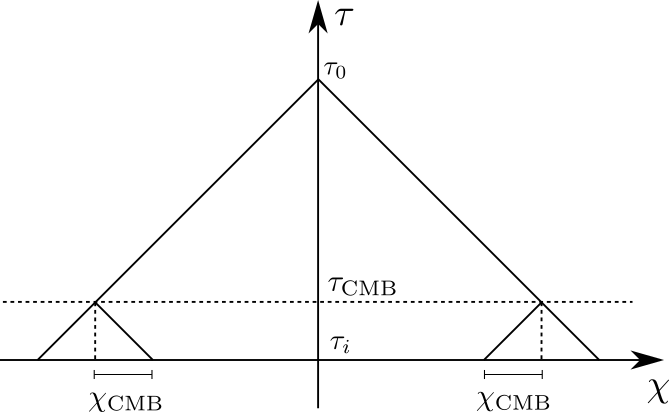
\includegraphics[width=0.7\textwidth]{horizon_problem.png}
	\caption{The horizon problem. According to the conventional big bang cosmology, different regions of the CMB we observe today have had no overlap in their particle horizon. Yet, the CMB is measured close to uniform everywhere.}
	\label{fig:horizon_problem}
\end{figure}

To resolve this issue, we need the particle horizon at recombination to be larger. The theory of cosmic inflation achieves this by having a period in the early universe where $3w+1<0$. In this case, we see from (\ref{eqn:particle_horizon_form}) that $\chi_\text{PH}$ is unbounded as $a_i \rightarrow 0$. The initial conformal time $\tau_i \rightarrow -\infty$, allowing enough proper time for the particle horizon growth. Then even the two opposite regions of the CMB we see can have had causal contact in the past, as depicted in Figure \ref{fig:horizon_solution}.
\begin{figure}[htbp!] 
	\centering    
	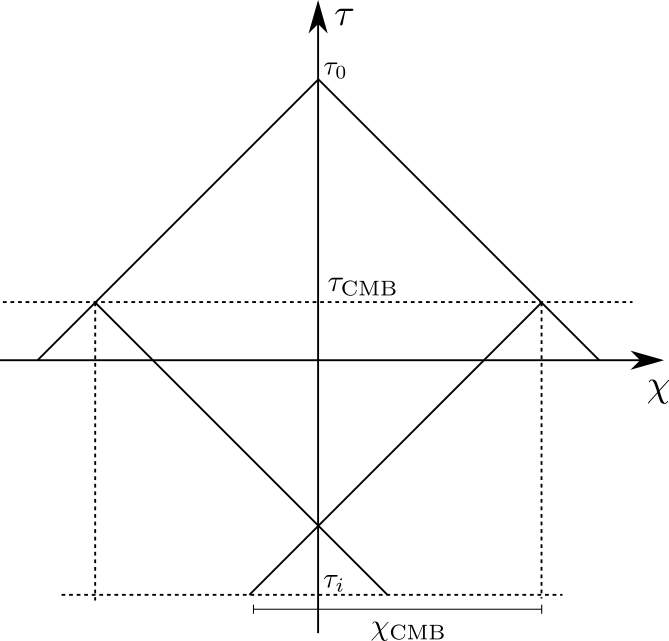
\includegraphics[width=0.6\textwidth]{horizon_solution.png}
	\caption{Solution to the horizon problem. Inflation allows more conformal time for different regions to have been in causal contact before recombination.}
	\label{fig:horizon_solution}
\end{figure}

Inflation can alternatively be characterised using the comoving Hubble radius defined as
\begin{align}
	\mathcal{H}^{-1} := \frac{1}{aH}.
\end{align}
Note that the particle horizon can then be expressed in terms of the comoving hubble radius as
\begin{align}
	\chi_\text{PH} = \int_{a_i}^{a_f} \frac{1}{a \dot{a}} da = \int_{\ln a_i}^{\ln a_f} \mathcal{H}^{-1} d\ln a. \label{eqn:particle_horizon_comoving_hubble}
\end{align}

The particle horizon represents the distance where objects could have \textit{ever} talked to each other. On the other hand, the comoving Hubble radius is a scale for how far information can reach \textit{now}. \footnote{Two points $\mathcal{H}^{-1}$ apart drifts away with relative physical velocity $v_\text{phys} = \dot{a} \mathcal{H}^{-1} = 1$, which is equal to $c$ in our units. It is difficult for such points to have causal interaction right now, especially within Hubble time $H^{-1}$.} As can be seen from (\ref{eqn:particle_horizon_form}), $\mathcal{H}^{-1} \propto a^{(3w_X+1)/2}$, which is $\propto a$ for radiation domination and $\propto a^{1/2}$ during matter domination.

Inflation explains the homogeneity of the observed CMB by requiring $\mathcal{H}^{-1}$ to have shrunk rapidly in early times; $d\mathcal{H}^{-1}/d\ln a < 0$. We find that $\ddot{a} > 0$, so the universe undergoes accelerated expansion. The steep decrease in $\mathcal{H}^{-1}$ is parametrised using a `slow-roll' parameter
\begin{align}
	\epsilon := - \frac{d\ln H}{d\ln a} = -\frac{\dot{H}}{H^2} \ll 1. \label{def:slow_roll_epsilon}
\end{align}
Inflation also needs to last long enough for the particle horizon to grow sufficiently large. We define another parameter to denote this constraint;
\begin{align}
	\eta := \frac{d\ln \epsilon}{d\ln a} = \frac{\dot{\epsilon}}{\epsilon H} \ll 1. \label{def:slow_roll_eta}
\end{align}


\subsection{Slow-roll inflation}
\label{section:slow-roll_inflation}

The simplest model of inflation consists of a single scalar field $\phi$. The action for a real scalar field with canonical kinetic term and potential $V(\phi)$ is given by
\begin{align}
	S_\phi = \int dt d^3 \vv{x} \; \sqrt{-g} \left[ -\frac{1}{2} g^{\mu\nu} \partial_\mu \phi \partial_\nu \phi - V(\phi) \right],		\label{eqn:real_scalar_field_action}
\end{align}
where $g:=\det g$. Denoting the integrand as the Lagrangian density $\Lagr[t, \vv{x}, \phi, \partial_\mu \phi]$, the energy-momentum tensor can be expressed using functional derivatives as
\begin{align}
	T_{\mu\nu} = \frac{-2}{\sqrt{-g}} \frac{\delta\Lagr}{\delta g^{\mu\nu}} = -2 \frac{\delta \Lagr}{\delta g^{\mu\nu}} + g_{\mu\nu} \Lagr.
\end{align}
Here, we used the identity $\delta\sqrt{-g} = -(1/2) \sqrt{-g} g_{\mu\nu} \delta g^{\mu\nu}$. Substituting (\ref{eqn:real_scalar_field_action}),
\begin{align}
	T_{\mu\nu} = \left( \partial_\mu \phi \right) \left( \partial_\nu \phi \right) + g_{\mu\nu} \left( -\frac{1}{2} g^{\rho\sigma} \partial_\rho \phi \partial_\sigma \phi - V(\phi) \right).
\end{align}
Now suppose that $\phi$ drives inflation in the FLRW background. Due to the symmetries present in the homogeneous and isotropic metric, the inflation field can only depend on time; $\phi(\vv{x}, t) = \bar{\phi}(t)$. We can read off the inflation field's energy density and pressure from the energy-momentum tensor.
\begin{align}
	\rho_{\bar{\phi}} =& -T^0_{\;\;0} = \frac{1}{2} \dot{\bar{\phi}}^2 + V(\bar{\phi}),	\\
	P_{\bar{\phi}} \delta^i_j =& T^i_{\;\;j} = \delta^i_j \left( \frac{1}{2} \dot{\bar{\phi}}^2 - V(\bar{\phi}) \right).
\end{align}
The two terms $\frac{1}{2} \dot{\bar{\phi}}^2$ and $V(\bar{\phi})$ can be interpreted as the kinetic and potential energy of the inflation field, respectively. The equation of state is also expressed in terms of the two;
\begin{align}
	w_{\bar{\phi}} = \frac{P_{\bar{\phi}}}{\rho_{\bar{\phi}}} = \frac{\frac{1}{2} \dot{\bar{\phi}}^2 + V(\bar{\phi})}{\frac{1}{2} \dot{\bar{\phi}}^2 - V(\bar{\phi})}.
\end{align}
It follows that $\bar{\phi}$ satisfies the condition $3w_{\bar{\phi}}+1<0$ required for inflation, as long as the potential energy dominates over kinetic energy.

The classical equations of motion are obtained from the Euler-Lagrange equation. After some calculations we obtain
\begin{align}
	\ddot{\bar{\phi}} + 3H\dot{\bar{\phi}} = - V'(\bar{\phi}). 	  \label{eqn:inflation_background_equation_of_motion}
\end{align}
Even though $\bar{\phi}$ is a field, its dynamics given in (\ref{eqn:inflation_background_equation_of_motion}) are identical to those of a particle rolling down a one-dimensional potential. Its movement should be slow for the kinetic energy to be much smaller than the potential, and hence the name `slow-roll' inflation.

The Friedmann equations (\ref{eqn:Friedmann_1}-\ref{eqn:Friedmann_2}) can now be expressed in terms of the background inflationary field.
\begin{align}
	H^2 =& \frac{8\pi G}{3} \left( \frac{1}{2} \dot{\bar{\phi}}^2 + V(\bar{\phi}) \right) \approx \frac{8\pi G}{3} V(\bar{\phi}), \label{eqn:inflation_Friedmann_1} \\
	\frac{\ddot{a}}{a} =& -\frac{8\pi G}{3} \left( \dot{\bar{\phi}}^2 - \frac{1}{2} V(\bar{\phi}) \right) \approx \frac{8\pi G}{3} V(\bar{\phi}), \label{eqn:inflation_Friedmann_2}
\end{align}
where the slow-roll approximations have been used in the last step. Taking the derivative of (\ref{eqn:inflation_Friedmann_1}) gives us $3H\dot{\bar{\phi}} \approx -V'$. The parameters defined as
\begin{align}
	\epsilon_V := \frac{1}{16\pi G} \left( \frac{V'}{V} \right)^2, \;\;\;
	\eta_V := \frac{1}{8\pi G} \frac{V''}{V},
\end{align}
are then shown to be small. Therefore the slow roll parameters from (\ref{def:slow_roll_epsilon}-\ref{def:slow_roll_eta}) satisfy
\begin{align}
	\epsilon \approx \epsilon_V \ll 1, \;\;\;\;\; \eta \approx -2\eta_V + 4\epsilon_V \ll 1.
\end{align}
We see that as long as the potential $V(\phi)$ is chosen such that $\epsilon_V, \eta_V \ll 1$, the field $\phi$ can drive a period of accelerated expansion. Here, $\bar{\phi}(t)$ acts as a clock; it measures the progress of inflation until $\epsilon$ eventually grows comparable to 1 and inflation ends.

\subsection{Quantum fluctuations} \label{section:quantum_fluctuations}

So far our considerations on the inflation field $\phi$ have been entirely classical. Moving on to quantum theory, field values are no longer fixed at each point in spacetime. The goal of this section is to quantify the statistical properties of these quantum fluctuations.

We assume that the metric remains unperturbed for simplicity. Gravity is coupled with perturbations of the inflation field in reality, but this approximation will still allow us to derive most of the crucial results. We further neglect any terms suppressed by slow-roll parameters.

We write the inflation field as a sum of the classical solution and perturbation;
\begin{align}
	\phi(\vv{x}, t) = \bar{\phi}(t) + \frac{v(\vv{x}, t)}{a(t)},	\label{eqn:inflation_perturbation_definition}
\end{align}
where the factor of $1/a$ has been introduced for later convenience. First rewriting the scalar field action (\ref{eqn:real_scalar_field_action}) in terms of conformal time,
\begin{align}
	S_\phi = \int d\tau d^3\vv{x} a(\tau)^2 \left[ \frac{1}{2} (\phi')^2 - \frac{1}{2}(\nabla\phi)^2 - a(\tau)^2 V(\phi) \right].
\end{align}
When we include perturbations, terms linear in $v$ vanish from the equations of motion of $\bar\phi$. Further removing terms with derivatives of $V(\phi)$ using the slow-roll condition,
\begin{align}
	\delta S_\phi =& \int d\tau d^3\vv{x} \left[ \frac{1}{2} \left(v' - \frac{a'}{a}v \right)^2 - \frac{1}{2}(\nabla v)^2 \right]	\\
	=& \int d\tau d^3\vv{x} \left[ \frac{1}{2} (v')^2 + \frac{1}{2}\frac{a''}{a} v^2 - \frac{1}{2}(\nabla v)^2 \right].
\end{align}
Integration by parts has been used to obtain the last line. The equations of motion for $v$ follows;
\begin{align}
	v'' - \frac{a''}{a} v - \nabla^2 v = 0.
\end{align}
Defining Fourier transforms of $v$ as
\begin{align}
	v(\vv{x},\tau) = \int \frac{d^3 \vv{k}}{(2\pi)^3} e^{i\vv{k} \cdot \vv{x}} \tilde{v}(\vv{k},\tau),
\end{align}
we obtain the Mukhanov-Sasaki equation;
\begin{align}
	v'' + (k^2 - \frac{a''}{a})v = 0.	\label{eqn:Mukhanov_Sasaki}
\end{align}
Tildes above $v$ have been omitted for brevity. Each $\vv{k}$ mode of the perturbative field $v(\vv{k},\tau)$ evolves independently from each other. During slow-roll inflation $a\propto-1/\tau$, and $a''/a = 2/\tau^2$. The general form of the solution is given by the \textit{mode functions} $v_k(\tau)$.
\begin{align}
	v_k(\tau) = c_+ \left( 1 - \frac{i}{k\tau} \right) e^{-ik\tau} + c_- \left( 1 + \frac{i}{k\tau} \right) e^{ik\tau}.
\end{align}

We would like to canonically quantise the field $v(\vv{k},\tau)$. To achieve this goal, we first convert from the Lagrangian to Hamiltonian formalism.
\begin{align}
	\pi :=& \frac{\partial \Lagr}{\partial v'} = v', \\
	\Hami :=& v'\frac{\partial \Lagr}{\partial v'} - \Lagr = \frac{1}{2} \pi^2 + \frac{1}{2} (\nabla v)^2 - \frac{1}{2} \frac{a''}{a} v^2 .
\end{align}
We now promote classical fields $v(\vv{k},\tau)$, $\pi(\vv{k},\tau)$ to operators $\hat{v}_\vv{k}(\tau)$, $\hat{\pi}_\vv{k}(\tau)$ satisfying equal-time commutation relations \footnote{This follows from its Fourier equivalent: $[\hat{v}(\vv{x}_1,\tau),\hat{\pi}(\vv{x}_2,\tau)] = i\delta^{(3)}(\vv{x}_1 - \vv{x}_2)$.}
\begin{align}
	\left[ \hat{v}_{\vv{k}_1}(\tau), \hat{\pi}_{\vv{k}_2}(\tau) \right] =& (2\pi)^3 \delta^{(3)}(\vv{k}_1 + \vv{k}_2), \\
	\left[ \hat{v}_{\vv{k}_1}(\tau), \hat{v}_{\vv{k}_2}(\tau) \right] =& \left[ \hat{\pi}_{\vv{k}_1}(\tau), \hat{\pi}_{\vv{k}_2}(\tau) \right] = 0.
\end{align}
Defining operators $\hat{a}_\vv{k}$ and $\hat{a}_\vv{k}^\dagger$ appropriately, we may write
\begin{align}
	\hat{v}_\vv{k} (\tau) =& v_k(\tau) \hat{a}_\vv{k} + v_k(\tau)^* \hat{a}_{-\vv{k}}^\dagger,  \\
	\hat{\pi}_\vv{k} (\tau) =& {v'_k}(\tau) \hat{a}_\vv{k} + {v'_k}(\tau)^* \hat{a}_{-\vv{k}}^\dagger.
\end{align}
As long as we normalise the mode functions $v_k(\tau)$ so that its Wronskian $W := v_k v'^*_k - v_k^* v'_k = i$ (purely imaginary since $v_k$ is real), we obtain
\begin{align}
	\left[ \hat{v}_{\vv{k}_1}(\tau), \hat{\pi}_{\vv{k}_2}(\tau) \right] =& i \left[ \hat{a}_{\vv{k}_1}, \hat{a}^\dagger_{\vv{k}_2} \right], \\
	\left[ \hat{a}_{\vv{k}_1}, \hat{a}^\dagger_{\vv{k}_2} \right] =& (2\pi)^3 \delta^{(3)}(\vv{k}_1 - \vv{k}_2).	\label{eqn:canonical_quantisation_commutation_relation_a}
\end{align}
The constructed $\hat{a}$ and $\hat{a}^\dagger$ are analogous to the creation and annihilation operators of a quantum harmonic oscillator. Our next step is to compute the Hamiltonian operator;
\begin{align}
	\hat{H} =& \int d^3 \vv{x} \left[ \frac{1}{2} \hat{\pi}^2 + \frac{1}{2} \left( \nabla \hat{v} \right)^2 - \frac{1}{2}\frac{a''}{a} \hat{v}^2 \right] \label{eqn:single_field_inflation_simple_hammiltonian}\\
	=& \int d^3 \vv{x} \frac{d^3 \vv{k}_1}{(2\pi)^3} \frac{d^3 \vv{k}_2}{(2\pi)^3} \frac{1}{2} e^{i(\vv{k}_1 + \vv{k}_2) \cdot \vv{x}}  \left[ \hat{\pi}_{\vv{k}_1} \hat{\pi}_{\vv{k}_2} - (\vv{k_1} \cdot \vv{k_2}) \hat{v}_{\vv{k}_1} \hat{v}_{\vv{k}_2} - \frac{a''}{a} \hat{v}_{\vv{k}_1} \hat{v}_{\vv{k}_2} \right] \\
	=& \int \frac{d^3 \vv{k}}{(2\pi)^3}  \frac{1}{2} \left[ \hat{\pi}_{\vv{k}} \hat{\pi}_{-\vv{k}} + k^2 \hat{v}_{\vv{k}} \hat{v}_{-\vv{k}} - \frac{a''}{a} \hat{v}_{\vv{k}} \hat{v}_{-\vv{k}} \right] \\
	=&  \int \frac{d^3 \vv{k}}{(2\pi)^3} \left[ E_k \left( \hat{a}_\vv{k} \hat{a}^\dagger_\vv{k} + \hat{a}^\dagger_{-\vv{k}} \hat{a}_{-\vv{k}} \right) + F_k \hat{a}_{\vv{k}} \hat{a}_{-\vv{k}} + F_k^* \hat{a}^\dagger_{\vv{k}} \hat{a}^\dagger_{-\vv{k}}  \right],
\end{align}
where
\begin{align}
	\omega_k^2 := k^2 - \frac{a''}{a}, \;\;\; E_k := \frac{1}{2}(|v'_k|^2 + \omega_k^2 |v_k|^2), \;\;\; F_k := \frac{1}{2}(v'^2_k + \omega_k^2 v^2_k).
\end{align}

Note that we are currently in the Heisenberg picture where the operators depend on time. Our mode functions have two degrees of freedom: $c_+$ and $c_-$. One of them has been fixed by the normalisation condition $W=2ik(|c_+|^2-|c_-|^2)=i$. The other degree of freedom remains, availing us a one-parameter family of possible initial mode functions. Note that $\hat{a}^\dagger_\vv{k}$ are defined in terms of $\hat{v}_\vv{k}$ and $\hat{\pi}_\vv{k}$. Fixing $\hat{a}_\vv{k}$ is thus equivalent to choosing $\hat{v}_\vv{k}$.

We define the vacuum $|\vv{0}\rangle$ to be the state satisfying $\hat{a}_\vv{k} |\vv{0}\rangle = 0$ for all $\vv{k} \in \mathbb{R}^3$. The expected energy of the vacuum state is given by
\begin{align}
	\langle \vv{0} | \hat{H} | \vv{0} \rangle =& \int \frac{d^3\vv{k}}{(2\pi)^3} E_k \langle \vv{0} | [ \hat{a}_\vv{k}, \hat{a}^\dagger_\vv{k} ] | \vv{0} \rangle	\\
	=& \int d^3\vv{k} E_k \delta^{(3)}(0),
\end{align}
where the divergence $\delta^{(3)}(0)$ arises only because we are integrating over the whole space. Removing this factor, we may interpret $E_k$ as the vacuum energy density for mode $k$.

We now ask the vacuum state to be a ground state of the Hamiltonian. Minimising the energy density $E_k$ while keeping normalisation condition $W=i$, we obtain the \textit{Bunch-Davies} mode function;
\begin{align}
	v_\vv{k}(\tau) = \frac{1}{\sqrt{2k}} \left( 1 - \frac{i}{k\tau} \right) e^{-ik\tau}. \label{eqn:bunch_davies_mode_function}
\end{align}
For this choice of mode function and vacuum, $E_k \rightarrow \hslash\omega_k/2$ as $\tau \rightarrow -\infty$. \footnote{$\hslash$ has been reinstated here for clarity.} This is analogous to the case of the quantum harmonic oscillator.

Lastly, we compute the zero-point fluctuation of the inflation field with respect to the vacuum. The two-point function follows from the commutation relation \eqref{eqn:canonical_quantisation_commutation_relation_a};
\begin{align}
	\langle \hat{v}_{\vv{k}_1} (\tau) \hat{v}_{\vv{k}_2} (\tau) \rangle &= \langle 0| [\hat{a}_{\vv{k}_1}, \hat{a}^\dagger_{-\vv{k}_2}] |0 \rangle \; v_{k_1}(\tau) v^*_{k_2}(\tau) \\
	&= (2\pi)^3 \delta^{(3)} (\vv{k}_1 + \vv{k}_2 ) \; P_{v}(k_1,\tau),   \label{eqn:single_field_inflation_power_spectrum}
\end{align}
where we defined the \textit{power spectrum} of $v$ as $P_v(k,\tau) := |v_k(\tau)|^2$. Fourier transforming back using
\begin{align}
	\hat{v}(\vv{x}, \tau) = \int \frac{d^3\vv{k}}{(2\pi)^3} \left[ v_k \hat{a}_\vv{k} + v^*_k \hat{a}^\dagger_\vv{k} \right] e^{i\vv{k} \cdot \vv{x}},
\end{align}
we compute the local variation in $v$;
\begin{align}
	\langle | \hat{v}(\vv{x}, \tau) |^2 \rangle =& \int \frac{d^3\vv{k}_1}{(2\pi)^3} \frac{d^3\vv{k}_2}{(2\pi)^3} \langle \vv{0} | v_{k_1} \hat{a}_{\vv{k}_1} v^*_{k_2} \hat{a}^\dagger_{\vv{k}_2} | \vv{0} \rangle 	\\
	=& \int \frac{d^3\vv{k}_1}{(2\pi)^3} \frac{d^3\vv{k}_2}{(2\pi)^3} v_{k_1} v^*_{k_2} \langle \vv{0} | \left[ \hat{a}_{\vv{k}_1}, \hat{a}^\dagger_{\vv{k}_2} \right] | \vv{0} \rangle	 \\
	=& \int \frac{d^3\vv{k}}{(2\pi)^3} |v_k|^2	\\
	=& \int d(\ln k) \mathcal{P}_v (k,\tau).
\end{align}
The dimensionless power spectrum is defined as
\begin{align}
	\mathcal{P}_v (k,\tau) := \frac{k^3}{2\pi^2} P_v(k,\tau).
\end{align}
Recall that perturbations in $\phi$ is given by $\delta\phi = v/a$ from (\ref{eqn:inflation_perturbation_definition}). The \textit{dimensionless power spectrum} for fluctuations in $\phi$ is therefore
\begin{align}
	\mathcal{P}_{\delta\phi} (k,\tau) = \frac{\mathcal{P}_v (k,\tau)}{a(\tau)^2} = \left( \frac{H}{2\pi} \right)^2 \left(1 + (k\tau)^2 \right),
\end{align}
where we used the fact that $a(\tau) = -1/H\tau$ during slow-roll inflation. For scales larger than the comoving Hubble radius we have $k\tau \ll 1$. In this limit, $\mathcal{P}_{\delta\phi} \rightarrow (H/2\pi)^2$ which is nearly constant. This is a key prediction from our simplistic model of inflation; we expect a nearly scale-invariant power spectrum of the primordial (end-of-inflation) perturbations.


\newpage
\section*{Summary}

In this introductory chapter, we covered the basic foundations of modern cosmology. Under a simplifying assumption that the universe is homogeneous and isotropic, we wrote down the most general metric tensor in which the scale factor $a(t)$ parametrises the expansion of the universe. We then considered radiation, matter and dark energy as the main constituents of the universe and derived Friedmann equations, which can be solved to determine the universe's expansion history given its energy composition. The universe likely began with a Big Bang and has been continuously expanding since. This led to another puzzle, the horizon problem; the early universe observed through the CMB seems exceptionally uniform despite supposedly having many causally disconnected regions. We discussed how inflation solves the problem by introducing a period of accelerated expansion shortly after the Big Bang, dramatically increasing the size of the particle horizon. Inflation also successfully provides a mechanism for generating the initial density fluctuations in the universe required to create the structure we observe today. We showed that quantum fluctuations in the inflation field follow a nearly scale-invariant spectrum which is consistent with observations to date.

The universe observed today is not quite homogeneous and isotropic at all scales. It is the distribution of inhomogeneities\textemdash perturbations about the homogeneous background\textemdash that contains valuable information about the universe and provides crucial observables for precision cosmology. We formulate the cosmological perturbation theory that describes the evolution of these primordial perturbations in the following chapter in the context of the CMB.\clearpage{}
\clearpage{}

\chapter{Cosmic Microwave Background Anisotropy}

\ifpdf
    \graphicspath{{Chapter2/Figs/Raster/}{Chapter2/Figs/PDF/}{Chapter2/Figs/}}
\else
    \graphicspath{{Chapter2/Figs/Vector/}{Chapter2/Figs/}}
\fi

The early universe consisted of hot plasma. Photons were tightly coupled to baryons through Compton scattering and remained in thermal equilibrium with them. Since the photon energy density dropped more rapidly with the universe's expansion compared to that of matter, the universe eventually transitioned from radiation-dominated to matter-dominated. Its temperature also continued to drop until it was low enough for the electrons and protons to combine and form neutral hydrogen. Following this rather abrupt event at redshift $\approx1100$, called \textit{recombination}, the photons no longer had electrons to scatter off from and instead started streaming freely through space. These photons are now observed by us today as the Cosmic Microwave Background (CMB).

The CMB follows a blackbody spectrum, since the radiation was in thermal equilibrium before it decoupled at recombination. Its temperature has been redshifted since then from approximately $3000$K to $T_\text{CMB}=2.725$K, which we observe today. Looking closer into the map of CMB temperature, there are fluctuations of order $10^{-5}$ that were seeded by the primordial perturbations and evolved subsequently in time. Such anisotropy in the CMB therefore contains valuable information about the universe.  Satellite surveys such as COBE \cite{Smoot1992cobe}, WMAP \cite{Spergel2003wmapfirst} and Planck \cite{PlanckCollaboration2013paramters}, as well as numerous ground-based experiments including ACT \cite{Dunkley2011act}, SPT \cite{Carlstrom2011spt}, and BICEP/Keck array \cite{Ade2016bicepkeck} have produced precise measurements of the CMB which have allowed us to constrain various cosmological parameters. The CMB anisotropy is the gold standard dataset for precision cosmology.

This chapter provides mathematical background and some physical intuitions for studying the CMB anisotropy, based on some standard materials on the topic including \cite{Dodelson2003textbook,Fergusson2020cosmology,Challinor2009lecture}. We start by taking a step forward from the homogeneous and isotropic universe discussed in the previous chapter and formulate the cosmological perturbation theory in Section \ref{section:the_inhomogeneous_universe}. Focussing on scalar perturbations we derive the linearised equations governing the time evolution of the perturbative variables in Section \ref{section:linearised_equations}. In Section \ref{section:CMB_anisotropy} we introduce the Boltzmann equation for photons and outline how it is solved numerically. We connect the primordial power spectrum to the angular power spectrum of the CMB anisotropy measured today.


\section{The inhomogeneous universe} \label{section:the_inhomogeneous_universe}

\subsection{Metric perturbations} \label{section:metric_perturbations}
Recall that the FLRW metric is given using conformal time by
\begin{align}
	ds^2 = a(t)^2 (-d\tau^2 + d\vv{x}^2).
\end{align}
We now perturb the metric as follows.
\begin{align}
	ds^2 = a(t)^2 \left[ -(1+2A) dt^2 + 2B_i \; d\tau dx^i + (\delta_{ij} + h_{ij}) dx^i dx^j \right].
\end{align}
The spatial indices $i,j,\cdots$ here are lowered and raised using $\delta_{ij}$. Note that the scale factor has not been perturbed, since any variation of it can be absorbed into other perturbative variables. There are 1, 3 and 6 degrees of freedom coming from $A$, $B_i$ and $h_{ij}$, respectively, adding up to 10 as expected from a metric tensor of the 3+1 dimensional spacetime.

We further extract the divergence part from $B_i$ and $h_{ij}$, as well as the trace of $h_{ij}$. Using $V$ and $T$ to denote vector and tensor quantities, 
\begin{align}
	B_i &= \partial_i B + B_i^V \\
	h_{ij} &= 2C \delta_{ij} + 2\partial_{\langle i}\partial_{j \rangle} E + (\partial_i E_j^V + \partial_j E_i^V). + 2E^T_{ij},
\end{align}
where $\partial_{\langle i}\partial_{j \rangle} := \partial_i \partial_j - \frac{1}{3} \delta_{ij} \nabla^2$.
The variables are chosen such that $B_i^V$ is divergence-free, while $h_{ij}^T$ is traceless and transverse.

The Scalar-Vector-Tensor (SVT) theorem states that to linear order in the perturbations, these modes decouple and evolve in three independent groups: scalars ($A,B,C,E$), vectors ($B_i^V,E_i^V$), and tensors ($E_{ij}^T$). These groups each contain 4, 4, and 2 degrees of freedom, again adding up to 10 as required. In this section, we are only interested in the scalar perturbations responsible for generating the temperature anisotropy and E-mode polarisation observed in the CMB. \footnote{Tensor modes also generate the temperature anisotropy and E-mode polarisation as well as B-mode polarisation, but their contributions are negligible compared to those of the scalar modes.} We will therefore set the vector and tensor modes of the perturbations to zero.

Keeping only the scalar modes, the perturbed metric becomes
\begin{align}
	ds^2 = a(\tau)^2 \left[ -(1+2A) dt^2 + 2 \partial_i B \; d\tau dx^i + \left( (1+2C)\delta_{ij} + 2\partial_{\langle i}\partial_{j \rangle} E \right) dx^i dx^j \right]. \label{eqn:perturbed_metric_scalar}
\end{align}

Coordinate transformations are \textit{gauge} symmetries in General Relativity; they correspond to redundancies in our mathematical representation of the system. Redefining the coordinate variables may change how the theory looks, but all physical results derived in the new set are equivalent to the original theory. These redundant degrees of freedom may still appear to evolve in a non-trivial manner and therefore need to be treated properly. Here, we outline how to fix a gauge in the perturbed metric and use gauge-invariant quantities to connect results from different gauges.

Consider the coordinate transformations $x^\mu \rightarrow \tilde{x}^\mu = x^\mu + \xi^\mu$ for some small $\xi$. As long as $\xi$ is of the same order as other perturbative variables, the background metric remains to be FLRW. We dcompose $\xi$ as above, keeping only the scalar perturbations. The transformations can then be described by two arbitrary functions $T$ and $L$ so that $\xi^0 = T(\tau,\vv{x})$ and $\xi^i = \partial_i L(\tau,\vv{x})$. The transformation matrices take the form
\begin{align}
	\frac{d\tilde{x}^\alpha}{dx^\mu} = \begin{pmatrix}
		1 + T' & \partial_i T \\ \partial_i L' & \delta_{ij} + \partial_i \partial_j L
	\end{pmatrix},
	\hspace{0.05\linewidth}
	\frac{dx^\mu}{d\tilde{x}^\alpha} = \begin{pmatrix}
		1 - T' & -\partial_i T \\ -\partial_i L' & \delta_{ij} - \partial_i \partial_j L
	\end{pmatrix}. \label{eqn:gauge_transformation_matrix}
\end{align}
The metric tensor in the new set of coordinates can be found using the tensor transformation rule
\begin{align}
	g_{\mu\nu} \rightarrow \tilde{g}_{\alpha\beta} = \frac{dx^\mu}{d\tilde{x}^\alpha} \frac{dx^\nu}{d\tilde{x}^\beta} g_{\mu\nu}.
\end{align}
Note also that the scale factor also changes under 
metric transforms due to variations in its argument;  $a(\tau)^2 \rightarrow a(\tilde{\tau})^2 = a(t)^2 (1 + 2 \mathcal{H} T)$ at first order in perturbations. After some calculations, we see that each perturbation variable in the metric \eqref{eqn:perturbed_metric_scalar} transforms like
\begin{alignat}{2}
	\tilde{A} &= A - T' - \mathcal{H}T, \qquad &&\tilde{B} = B + T - L', \label{eqn:gauge_transform_perturbations_1}\\
	\tilde{C} &= C - \mathcal{H}T - \frac{1}{3}\nabla^2 L, \qquad &&\tilde{E} = E - L. \label{eqn:gauge_transform_perturbations_2}
\end{alignat}
Hence, the two free functions $T$ and $E$ can be chosen in a way that the metric perturbations satisfy some desirable properties containing two degrees of freedom. Doing so \textit{fixes} the gauge and no further redundancies remain in our formulation. Popular choices include the \textit{spatially flat} gauge, where $C=E=0$ and the spatial perturbations vanish as $h_{ij}=0$, and the \textit{synchronous} gauge, for which $A=B=0$ and the time is left unperturbed.

Results from different gauge choices may appear dissimilar. In order to link them together, it is convenient to work with quantities constructed from the perturbative variables such that they remain invariant under the transformations \eqref{eqn:gauge_transform_perturbations_1}-\eqref{eqn:gauge_transform_perturbations_2}. The Bardeen potentials are two such examples of gauge-invariant variables;
\begin{align}
	\Psi_\textrm{B} &:= A + \mathcal{H}(B-E') + B' - E'', \\
	\Phi_\textrm{B} &:= -C - \mathcal{H}(B-E') + \frac{1}{3}\nabla^2 E.
\end{align}

The gauge we will be using for the rest of this chapter is the \textit{Newtonian} gauge where $B=E=0$. This allows us to identify $A$ and $C$ with the Bardeen potentials, and the metric takes the form (dropping the subscript)
\begin{align}
	ds^2 = a(\tau)^2 \left[ -(1 + 2\Psi) d\tau^2 + (1-2\Phi) d\vv{x}^2  \right]. \label{eqn:perturbed_metric_newtonian_gauge}
\end{align}
The perturbations $\Psi(\tau,\vv{x})$ and $\Phi(\tau,\vv{x})$ are directly related to the classical gravitational potential in the Newtonian limit.


\subsection{Matter perturbations}

In order to complete the Einstein field equation, we need the energy-momentum tensor as well as the metric written to first order in perturbations. Recall that a perfect fluid in a homogeneous universe has $\bar{T}_{\mu\nu} = (\bar{\rho} + \bar{P}) \bar{U}_\mu \bar{U}_\nu + \bar{P} \bar{g}_{\mu\nu}$. The perturbations in $T_{\mu\nu}$ come from two sources: a) directly from perturbations in the energy density and pressure, and b) indirectly through variations in the metric and comoving observer's four-velocity. We consider the local inertial frame to separate these two effects. Let
\begin{align}
	(E_0)^\mu := a^{-1} (1 - \Psi) \delta^\mu_0, \quad (E_i)^\mu := a^{-1} (1 + \Phi) \delta^\mu_i. \label{eqn:newtonian_gauge_tetrad}
\end{align}
The four vectors above form an orthonormal frame where $g_{\mu\nu}(E_\alpha)^\mu (E_\beta)^\nu = \eta_{\alpha\beta}$. In this locally-Minkowski frame, each component of the tensor $\tilde{T}^{\alpha\beta}$ represent a physical property of the fluid. We write
\begin{align}
	&\tilde{T}^{00} = \rho = \bar{\rho} + \delta\rho, \qquad \tilde{T}^{0i} = q^i = (\bar{\rho}+\bar{P})v^i, \\
	&\tilde{T}^{ij} = P \delta^{ij} - \Pi^{ij} = (\bar{P} + \delta P) \delta^{ij} - \Pi^{ij}.
\end{align}
The momentum density $\vv{q}$ and the mean velocity $\vv{v}$ are first-order quantities which vanish in the absence of perturbations. The symmetric and traceless matrix $\Pi^{ij}$ represents anisotropic stress. This quantity vanishes for non-relativistic fluids such as dark matter, while it remains small but non-zero for relativistic particles like photons.

Transforming back to the original coordinates through $T^{\mu\nu}=(E_\alpha)^\mu (E_\beta)^\nu \tilde{T}^{\alpha\beta}$, we get
\begin{alignat}{2}
	T^{00} &= a^{-2} \bar{\rho} &&\;\;+ a^{-2}\left( \delta\rho - 2\Psi\bar{\rho} \right), \label{eqn:perturbed_energy_momentum_tensor_1}\\
	T^{0i} &= 0 &&\;\;+ a^{-2} q^i, \label{eqn:perturbed_energy_momentum_tensor_2}\\
	T^{ij} &= a^{-2} \bar{P} \delta^{ij} &&\;\;+ a^{-2} \left[ (\delta P + 2\Phi\bar{P})\delta^{ij} - \Pi^{ij} \right],\label{eqn:perturbed_energy_momentum_tensor_3}
\end{alignat}
at first order in perturbations. Note that when only the scalar modes are considered, we may write $v^i = \partial_i v$ and $\Pi^{ij} = \partial_{\langle i} \partial_{j \rangle} \Pi$ for some $v$ and $\Pi$. If multiple fluids contribute, then the total energy-momentum tensor can be obtained by summing over the individual values for each constituent $I$; $\delta\rho = \sum_I \delta\rho_I$, $\delta P = \sum_I \delta P_I$, and $\delta \vv{q} = \sum_I \vv{q}_I$.

The energy-momentum tensor is also subject to the gauge transformations \eqref{eqn:gauge_transformation_matrix}. Each perturbation variable appearing in $\delta T^{\mu\nu}$ transforms as
\begin{align}
	\tilde{\delta\rho} &= \delta\rho - T\bar{\rho}',  &&\tilde{\delta P} = \delta P -T\bar{P}', \label{eqn:gauge_transform_perturbations_3}\\
	\tilde{q}^i &= q^i + (\bar{\rho} + \bar{P})L',  &&\tilde{\Pi}^{ij} = \Pi^{ij}. \label{eqn:gauge_transform_perturbations_4}
\end{align}
We may therefore choose to work in a gauge where some of the above vanish. For example, $\delta \rho = B = 0$ in \textit{uniform density} gauge, and spatial slices of the fluid have constant energy density.


\subsection{Initial perturbations}

With the metric and matter perturbations written down, we only need one more ingredient to solve the linearised Einstein's equations: initial conditions. In inflationary $\Lambda$CDM, deviations from the background solution originate from the quantum fluctuations of the inflation field as we discussed in Section \ref{section:quantum_fluctuations}. Statistical properties of the perturbations' distribution depend on the details of the inflationary scenario.

In models where a single-field drives inflation, such as slow-roll inflation, the field can be thought of as a local \textit{clock}. Classical equations of motions dictate the trajectory followed by the field, which then regulates the expansion of the universe. The spatial fluctuations of the inflation field can therefore be considered as the differences in how far the field has moved down the trajectory at each point in space. Any such perturbations can be determined solely from the variations in the local `clock' time $\delta\tau(\tau,\vv{x})$;
\begin{align}
	\delta f \;=\; \bar{f}(\tau + \delta\tau, \vv{x}) - \bar{f}(\tau,\vv{x}) \;=\; \frac{\partial\bar{f}}{\partial\tau} \delta\tau, \label{eqn:local_clock_time_fluctuation}
\end{align}
for any $f$. By substituting $f=\rho_I$ and $P_I$ we find that $\delta\rho_I/\bar{\rho}'_I = \delta P_I / \bar{P}'_I = \delta\tau$, which is locally constant for each constituent $I$. Combined with the background continuity equation \eqref{eqn:continuity},
\begin{align}
	\frac{\delta_I}{1+w_I} = \frac{\delta_J}{1+w_J}, \label{eqn:adiabatic_modes_density_contrast}
\end{align}
where we have defined the density contrast as $\delta_I := \delta\rho_I / \bar{\rho}_I$. \footnote{To avoid confusion with the differential operator and Dirac delta function, we always write the density contrast $\delta_I$ with a subscript $I$ indicating which fluid it represents. The \textit{total} density contrast will be denoted as $\delta_{tot}$.} In particular, $\delta_r = (4/3) \delta_m$ at each point $\vv{x}$. Furthermore, for a fluid with a constant equation of state $w_I = \bar{P_I} / \bar{\rho_I}$, the \textit{sound speed} $c_s$ is defined as
\begin{align}
	c_s^2 := \frac{\delta P_I}{\delta\rho_I} = \frac{\bar{P}'_I}{\bar{\rho}'_I} = \frac{d\bar{P}_I}{d\bar{\rho}_I} = w_I. \label{eqn:adiabatic_modes_sound_speed}
\end{align}
Hence, the perturbed energy density and pressure also satisfy the equation of state; $P_I = w_I \rho_I$.

Perturbations satisfying the strong constraint of \eqref{eqn:adiabatic_modes_density_contrast} are called to be \textit{adiabatic}. They affect every component of the universe equally so that the ratio between density contrasts is uniform in space. Orthogonal to adiabatic modes are \textit{isocurvature} modes where the total density contrast vanishes everywhere and $\delta_r = -\delta_m$ at the end of inflation. Some multi-field inflation models are expected to seed isocurvature perturbations. However, all observations so far are consistent with purely adiabatic initial conditions \cite{Kogut2003wmapAdiabatic, PlanckCollaboration2018inflation}.

\section{Linearised equations} \label{section:linearised_equations}

In this section, we derive equations governing the time evolution of the perturbations defined in the previous section. The equations are of first order in the perturbative variables. Although all calculations here are performed in the Newtonian gauge, the methodology illustrated here is general and applies to any choice of gauge. In order to avoid conflicting notations later, we use $\eta$ instead of $\tau$ for conformal time in this section. \footnote{Unfortunately, we could not have avoided the clash by using $\eta$ to denote conformal time to begin with, since $\eta$ is also commonly used as one of the slow-roll parameters in inflation.}

\subsection{Kinematics}

Non-interacting perfect fluids such as cold dark matter are \textit{conserved}; they should satisfy the perturbed metric's equivalent of the continuity equation \eqref{eqn:continuity}, as well as the Euler equations regarding time evolution of the perturbative velocity field $\vv{v}(\eta,\vv{x})$. In this section, we derive the conservation equations for the perturbation theory using the constraint $\nabla_\nu {T^\nu}_\mu = 0$.

The first step is to compute the Christoffel symbols \eqref{def:Levi_Civita}. Working in Newtonian gauge, they are given by
\begin{alignat}{6}
	&\Gamma^{0}_{00} &&= \mathcal{H} \;\;&&+ \Psi', \qquad &&\Gamma^{0}_{i0} &&= 0 \;\;&&+ \partial_i\Psi', \label{eqn:perturbed_christoffel_symbols_1}\\
	&\Gamma^{0}_{ij} &&= \mathcal{H}\delta_{ij} \;\;&&- \left[\Phi' + 2\mathcal{H}(\Psi+\Phi) \right]\delta_{ij}, \qquad &&\Gamma^{i}_{00} &&= 0 \;\;&&+ \partial_i\Psi, \label{eqn:perturbed_christoffel_symbols_2}\\
	&\Gamma^{i}_{jk} &&= 0 \;\;&&+ (\partial_k \Phi)\delta_{ij} - (\partial_i \Phi)\delta_{jk} - (\partial_j \Phi)\delta_{ik}, \qquad &&\Gamma^{i}_{j0} &&= \mathcal{H}\delta_{ij} \;\;&&- \Phi'\delta_{ij}. \label{eqn:perturbed_christoffel_symbols_3}
\end{alignat}
The background values appear as the first term in each equation. Note that these look different to \eqref{eqn:homogenous_christoffel_1}-\eqref{eqn:homogenous_christoffel_3} because the conformal time $\eta$ is used here instead of the comoving time $t$. Spatial indices are lowered and raised using the delta function above.

There are four components in the equation $\nabla_\nu {T^\nu}_\mu = \partial_\nu {T^\nu}_\mu + \Gamma^\nu_{\nu\gamma} {T^\gamma}_\mu - \Gamma^\gamma_{\nu\mu} {T^\nu}_\gamma=0$. We take $\mu=0$ and substitute in the perturbed energy-momentum tensor \eqref{eqn:perturbed_energy_momentum_tensor_1}-\eqref{eqn:perturbed_energy_momentum_tensor_3}. After removing the background part $\bar{\rho}'=-3\mathcal{H}(\bar{\rho}+\bar{P})$, we obtain
\begin{align}
	(\delta\rho)' + \nabla \cdot \vv{q}+ 3 \mathcal{H} (\delta\rho + \delta P) - 3 \Phi' (\bar{\rho} + \bar{P})  = 0.  \label{eqn:perturbed_continuity_equation}
\end{align}
This is the continuity equation. Only the first two terms would be present if the spacetime were flat; any changes in the energy density perturbation $\delta\rho$ are then due to the fluid flow parametrised by the momentum density $\vv{q} = (\bar{\rho}+\bar{P})\vv{v}$. The third term accounts for the dilution of the fluid density from the expansion of the universe. The last term corrects for the perturbations in the expansion, where $\Phi'$ comes from the time derivative of the effective spatial scale factor $a(\eta)(1-\Phi(\eta,\vv{x}))$. All factors of 3 here originate from having three spatial dimensions.

\eqref{eqn:perturbed_continuity_equation} applies to every fluid component which does not interact with others. Rewriting in terms of the equation of state $w_I = \bar{P}_I / \bar{\rho}_I$, sound speed $c_s^2 = \delta P / \delta\rho$, and density contrast $\delta_I = \delta\rho_I / \bar{\rho}_I$, we have
\begin{align}
	\delta'_I + (1+w_I) \nabla\cdot\vv{v}_I + 3\mathcal{H}(c_s^2-w_I)\delta_I - 3(1+w_I) \Phi' = 0.
\end{align}
This is a first-order differential equation for $\delta_I$.

Meanwhile, the $\mu=i$ part of $\nabla_\nu {T^\nu}_\mu =0$ yields the Euler equations;
\begin{align}
	\vv{v}'_I + \mathcal{H} \left( 1 - \frac{3\bar{P}'}{\bar{\rho}'} \right) \vv{v}_I + \frac{\nabla(\delta P)}{\bar{\rho} + \bar{P}} + \nabla\Psi = 0. \label{eqn:perturbed_Euler_equation}
\end{align}
We do not have the zeroth order terms in this case since $\vv{v}=\vv{0}$ in the homogeneous universe. Although \eqref{eqn:perturbed_Euler_equation} is a vector equation, it has only one independent scalar component after rewriting $\vv{v}=\nabla v$ for some $v$. This is because we are only considering the scalar perturbations.

The physical meaning of the individual terms in \eqref{eqn:perturbed_Euler_equation} is as follows. The second term with a factor of $\mathcal{H}$ represents the dilution, or redshift, of the velocity due to the universe's expansion. The third relates to the pressure; the fluid's velocity accelerates in the direction of the steepest pressure gradient. Lastly, the gravitational force pulling towards a potential well is encapsulated in the final term.

If we assume adiabatic initial conditions where $\bar{P}'/\bar{\rho}' = \delta P / \delta \rho = c^2_s$, then the Euler equation further simplifies to
\begin{align}
	\vv{v}'_I + \mathcal{H} (1 - 3c^2_s) \vv{v}_I + \frac{c^2_s}{1+w_I} \nabla\delta_I + \nabla\Psi = 0,
\end{align}
for a given fluid component $I$.


\subsection{Dynamics}

Our next step is to solve the linearised Einstein's equations. Using the Christoffel symbols \eqref{eqn:perturbed_christoffel_symbols_1}-\eqref{eqn:perturbed_christoffel_symbols_3}, we may calculate the Einstein tensor for the perturbed metric. After a rather long but straightforward algebra,
\begin{alignat}{2}
	G_{00} &= 3\mathcal{H}^2 \quad&&+ 2\nabla^2 \Phi - 6 \mathcal{H} \Phi', \label{eqn:perturbed_einstein_tensor_1}\\
	G_{0i} &= 0 \quad&&+ 2\partial_i \Phi' + 2 \mathcal{H} \partial_i \Psi, \label{eqn:perturbed_einstein_tensor_2}\\
	G_{ij} &= -(2\mathcal{H}' + \mathcal{H}^2) \delta_{ij} \quad&&- \partial_{\langle i} \partial_{j \rangle} (\Psi - \Phi) + \left[ \frac{2}{3}\nabla^2 (\Psi-\Phi) + 2\Phi'' \right. \nonumber\\
	& &&\quad + (4\mathcal{H}' + 2\mathcal{H}^2)(\Psi+\Phi) + 2\mathcal{H}\Psi' + 4\mathcal{H}\Phi' \biggr] \delta_{ij}, \label{eqn:perturbed_einstein_tensor_3}
\end{alignat}
where we have separated the zeroth and first order terms as before.

Einstein's equations, $G_{\mu\nu} = 8\pi G T_{\mu\nu}$, consists of 10 parts. Among these only 4 of them relate to scalar modes, similarly to how there are 4 independent scalar perturbations in the metric tensor \eqref{eqn:perturbed_metric_scalar}. We obtain one equation for each of $G_{00}$, $G_{i0}$, the trace of $G_{ij}$, and lastly the trace-free part of $G_{ij}$.

We start with the trace-free component of $G_{ij}$. Combining  \eqref{eqn:perturbed_einstein_tensor_3} and \eqref{eqn:perturbed_energy_momentum_tensor_3} gives
\begin{align}
	-\partial_{\langle i} \partial_{j \rangle} (\Psi - \Phi) = \partial_{\langle i} \partial_{j \rangle} \Pi.
\end{align}
The anisotropic stress $\Pi$ is negligible in reality. Non-relativistic matter does not contribute at all to $\Pi$, and photons induce non-zero but small anisotropic stress. Hence, we set $\Pi\approx 0$ and let $\Psi = \Phi$ for the rest of our derivations.

The $00$, $i0$, and $ij$ trace parts of Einstein's equations then take the form
\begin{align}
	\nabla^2 \Phi - 3 \mathcal{H} \Phi' - 3\mathcal{H}^2 \Phi &= 4\pi G \; a^2 \delta\rho, \label{eqn:perturbed_einstein_equations_1}\\
	\Phi' + \mathcal{H} \Phi &= -4\pi G \; a^2 q, \label{eqn:perturbed_einstein_equations_2}\\
	\Phi'' + 3\mathcal{H} \Phi' + (2\mathcal{H}' + \mathcal{H}^2) \Phi &= 4\pi G \; a^2 \delta P. \label{eqn:perturbed_einstein_equations_3}
\end{align}
We used the background equations to remove terms of zeroth order in perturbations. The $i0$ part generally gives a vector identity but it only has one scalar degree of freedom since $\vv{q}=(\bar{\rho}+\bar{P})\vv{v} = \nabla q$ for some $q := (\bar{\rho}+\bar{P}) v$.

Time derivatives of $\Phi$ on the left-hand side can be removed by putting \eqref{eqn:perturbed_einstein_equations_1} and \eqref{eqn:perturbed_einstein_equations_2} together. The result is Poisson's equation;
\begin{align}
	\nabla^2 \Phi = 4\pi G \; a^2 (\delta\rho - 3\mathcal{H}q). \label{eqn:perturbed_poisson_eqution}
\end{align}
This resembles Poisson's equation for Newtonian gravity: $\nabla^2 \phi_{\text{Newt.}} = 4\pi G \; \rho$. We confirm our previous claim that $\Phi$ corresponds to the perturbations of the Newtonian gravitational potential. Note that \eqref{eqn:perturbed_poisson_eqution} is best solved in Fourier space where $\nabla^2\Phi(\eta,\vv{x})$ reduces to $-k^2 \tilde{\Phi}(\eta,\vv{k})$.


\subsection{Curvature perturbations} \label{section:curvature_perturbations}

The Bardeen potential $\Phi_B$ is an extremely useful quantity for studying cosmological perturbation theory. It is not only gauge-invariant but also representative of a physically meaningful quantity\textemdash gravitational potential\textemdash in Newtonian gauge which can be solved using the Poisson's equation \eqref{eqn:perturbed_poisson_eqution}. Gauge-invariant quantities also let us connect results from different gauge choices in a consistent manner.

Another gauge-invariant variable which plays a crucial role in cosmology is the constant density curvature perturbation, or simply \textit{curvature perturbation}, defined as
\begin{align}
	\zeta := - C + \frac{1}{3} \nabla^2 E + \mathcal{H} \frac{\delta\rho}{\bar{\rho}'}. \label{def:curvature_perturbation}
\end{align}
The name originates from the fact that it closely relates to the spatial curvature $R^{(3)}$ in the uniform density gauge $B=\delta\rho=0$. In Newtonian gauge,
\begin{align}
	\zeta = \Phi + \mathcal{H}\frac{\delta\rho}{\bar{\rho}'} = \Phi - \frac{\delta\rho}{3(\bar{\rho}+\bar{P})},
\end{align}
where we used the background continuity equation $\bar{\rho}'=-3\mathcal{H}(\bar{\rho}+\bar{P})$ for the second equality. The time derivative of $\zeta$ can then be evaluated using \eqref{eqn:perturbed_continuity_equation}:
\begin{align}
	\zeta' &= \Phi' + \left[ \frac{1}{3}\nabla\cdot\vv{v} + \mathcal{H}\frac{\delta\rho + \delta P}{\bar{\rho} + \bar{P}} - \Phi' \right] + \frac{\delta\rho (\bar{\rho}' + \bar{P}')}{3(\bar{\rho}+\bar{P})^2}  \label{eqn:zeta_time_derivate_1} \\
	&= \frac{1}{3}\nabla^2 v + \frac{\mathcal{H}}{\bar{\rho} + \bar{P}} \left( \delta P - \frac{\bar{P}'}{\bar{\rho}'} \delta\rho \right). \label{eqn:zeta_time_derivate_2}
\end{align}
The second term in \eqref{eqn:zeta_time_derivate_2} vanishes for the adiabatic modes sourced by single-field inflation, as long as we assume the constant equations of state shown in \eqref{eqn:adiabatic_modes_sound_speed}. We are then left with $\zeta' = (1/3) \nabla^2 v$.

Now consider scales much larger than the comoving Hubble radius $\mathcal{H}^{-1}$, namely the `super-horizon' scales. The Fourier space equivalent of this condition is $k \ll \mathcal{H}$. The Fourier transform of $\nabla^2 v$ equals $-k^2 \tilde{v}$, which is much smaller than the typical time scale $\mathcal{H}$ in this limit. It follows that $\zeta'\approx 0$; curvature perturbations are conserved in super-horizon scales.

For this reason, the curvature perturbations play a major role in connecting inflation to the primordial initial conditions. Recall that the comoving Hubble radius $\mathcal{H}^{-1}$ shrinks during inflation due to exponential growth of the universe. Most physical scales of interest that were originally sub-horizon, or $k^{-1}\gg \mathcal{H}^{-1}$, eventually exit the horizon as $\mathcal{H}^{-1}$ drops below $k^{-1}$. After the end of inflation, $\mathcal{H}^{-1}$ grows back so that the modes can re-enter the horizon. Here, since $\zeta$ remains constant at super-horizon scales, the value of $\zeta$ at horizon re-entry is equal to that evaluated at the time the mode left the horizon. $\zeta$ serves as a bridge which links the quantum fluctuations generated during inflation to the initial perturbations after inflation.


\section{CMB anisotropy} \label{section:CMB_anisotropy}

The linearised Einstein field equations \eqref{eqn:perturbed_einstein_equations_1}-\eqref{eqn:perturbed_einstein_equations_3} dictate the time evolution of the gravitational perturbations given the total energy, momentum, and pressure of the universe's constituents. The cold dark matter's contributions to these quantities can be solved using the perturbed continuity equation \eqref{eqn:perturbed_continuity_equation} and Euler equations \eqref{eqn:perturbed_Euler_equation}. This section covers how perturbations in the photon temperature evolve and translate into the observed CMB anisotropy, the main cosmological dataset of our interest.

Studying photon perturbations is similar in principle to cold dark matter but involves two major complications. First, photons interact directly with baryons through Compton scattering. Their perturbations hence stay tightly coupled until recombination, when the electrons and protons combine to form neutral hydrogen and the photons start free-streaming instead. We outline in Section \ref{section:boltzmann_equations} how the Boltzmann equations are used to find the time evolution of photon perturbations while accounting for the scattering effects. Second, unlike cold dark matter whose perturbations are characterised by its density contrast $\delta\rho_m$ and velocity field $\vv{v}_m$, we require a whole hierarchy of functions to accurately describe photons. This is because the photons do not necessarily travel parallel to the wavevector when perturbed; $\vv{p} \nparallel \vv{k}$. We discuss the details in Section \ref{section:boltzmann_hierarchy}.


\subsection{Boltzmann equations} \label{section:boltzmann_equations}
\subsubsection*{Photons}

We start by calculating the path a photon takes while free-streaming within the perturbed metric \eqref{eqn:perturbed_metric_newtonian_gauge}. The 4-momentum of a photon in local coordinates satisfies $\eta_{\alpha\beta}\tilde{P}^\alpha \tilde{P}^\beta = 0$ since photons are massless. We may hence write its components as
\begin{align}
	\tilde{P}^0 = p, \qquad \tilde{P}^i = p \hat{p}^i,
\end{align}
where $\hat{\vv{p}}$ is a unit vector indicating the direction of propagation and $p$ is the magnitude of the 3-momentum. We can revert back to the perturbed metric using the tetrad in \eqref{eqn:newtonian_gauge_tetrad}; since $P^\mu = (E_\alpha)^\mu \tilde{P}^\alpha$,
\begin{align}
	P^0 = a^{-1} (1 - \Psi)p, \qquad P^i = a^{-1}(1 + \Phi) p \hat{p}^i. \label{eqn:perturbed_photon_four_momentum}
\end{align}
Recall that the 4-momentum is defined as $P^\mu = dx^\mu/\lambda$ for some affine parameter $\lambda$. Using our definition above,
\begin{align}
	\frac{dx^i}{d\eta} =  \frac{dx^i}{d\lambda} \frac{d\lambda}{d\eta} = \frac{P^i}{P^0} = (1+\Psi+\Phi)\hat{p}^i	\label{eqn:perturbed_photon_position_total_derivative}
\end{align}
to first order in perturbations. A comoving observer finds photons to be travelling more slowly while passing through overdense regions with $\Psi,\Phi<0$.

The geodesic equation \eqref{eqn:geodesic} takes the form
\begin{align}
	\frac{dP^\mu}{d\lambda} + \Gamma^\mu_{\nu\rho} P^\nu P^\rho = P^0 \left( \frac{dP^0}{d\eta} \right) + \Gamma^0_{\nu\rho} P^\nu P^\rho = 0.  \label{eqn:geodesic_equation_four_momentum}
\end{align}
Meanwhile, differentiating \eqref{eqn:perturbed_photon_four_momentum} gives
\begin{align}
	\frac{dP^0}{d\eta} = \frac{1-\Psi}{a} \left( \frac{dp}{d\eta} - \mathcal{H}p \right) - \frac{p}{a} \left( \frac{\partial\Psi}{\partial\eta} + \frac{dx^i}{d\eta} \frac{\partial\Psi}{\partial x^i}  \right). \label{eqn:perturbed_energy_total_derivative}
\end{align}
Note that the total derivative $d/d\eta$ here is taken along the trajectory $x^\mu = x^\mu(\eta)$ of the photon. We may combine \eqref{eqn:geodesic_equation_four_momentum} and \eqref{eqn:perturbed_photon_four_momentum} to obtain an expression for the total derivative of $p$;
\begin{align}
	\frac{1}{p} \left( \frac{dp}{d\eta} \right) = - \mathcal{H} + \Phi' - \hat{p}^i \partial_i \Psi. \label{eqn:perturbed_p_total_derivative}
\end{align}
Only the first term on the right-hand side is present at the zeroth order in perturbations, where we get $p\propto a^{-1}$. We confirm that photons are redshifted as the universe expands, justifying the definition of the redshift $z$ in \eqref{def:redshift}. The other two terms quantify the effect of gravitational perturbations on photon energy. Photons at a place where the potential is increasing over time \textit{gain} energy $\propto\Phi'$. On the other hand, photons moving out of a potential well \textit{lose} energy $\propto({\vv{p}}\cdot\nabla)\Psi$. Dividing by $p$ gives the last term in \eqref{eqn:perturbed_p_total_derivative}.


\subsubsection*{Distribution function} \label{section:distribution_function}

In order to fully understand the physical properties of photon perturbations, we need to study their distribution function $f(\eta,\vv{x},\vv{p})$ which measures the number of particles in a unit phase space volume. Photons in a thermal equilibrium within the homogenous universe follow the Bose-Einstein distribution where   
\begin{align}
	\bar{f}(\eta, p) = \left[ \exp \left\{ \frac{p}{\bar{T}(\eta)} \right\} - 1 \right]^{-1}, \label{eqn:photon_distribution_function}
\end{align}
up to a factor and the Boltzmann constant, both of which we set to $1$ for convenience. This is equivalent to the blackbody radiation with temperature $\bar{T}(\eta)$.

We define the fractional temperature anisotropy $\Theta$ by perturbing the photon distribution function as follows;
\begin{align}
	f(\eta, \vv{x}, p, \hat{\vv{p}}) = \left[ \exp \left\{ \frac{p}{\bar{T}(\eta)\left[1 + \Theta (\eta,\vv{x},\hat{\vv{p}}) \right]} \right\} - 1 \right]^{-1}. \label{eqn:perturbed_photon_distribution_function}
\end{align}
We have made an implicit assumption here that $\Theta(\eta,\vv{x},\hat{\vv{p}})$ does not depend on $p$, the photon energy. This claim will be justified later as we show that the Thomson scattering between photons and electrons leaves the energy of photons virtually unchanged.

The distribution function \eqref{eqn:perturbed_photon_distribution_function} can be expanded to linear order in perturbations as
\begin{align}
	f = \bar{f} - \frac{\partial \bar{f}}{\partial (\ln p)} \; \Theta,  \label{eqn:perturbed_photon_distribution_function_expansion}
\end{align}
by replacing $p$ with $p(1-\Theta)$ in \eqref{eqn:photon_distribution_function}. The temperature anisotropy $\Theta$ therefore closely relates to perturbations in the distribution function.

\subsubsection*{Collisionless equations} \label{section:collisionless_equation}

Liouville's theorem states that the phase space distribution function remains constant along the system's classical trajectories. A generalisation of this to systems with collisions is the Boltzmann equation. For our photon distribution function, it reads
\begin{align}
	\frac{df}{d\eta} &= \frac{\partial f}{\partial \eta} + \frac{\partial f}{\partial x^i}\frac{dx^i}{d\eta} + \frac{\partial f}{\partial(\ln  p)}\frac{d(\ln p)}{d\eta} + \frac{\partial f}{\partial \hat{p}^i}\frac{d\hat{p}^i}{d\eta} \label{eqn:boltzmann_equation_base}\\
	&= \left. \frac{df}{d\eta} \right|_\text{scattering} . \label{eqn:boltzmann_equation_base_scattering}
\end{align}
In \eqref{eqn:boltzmann_equation_base} we used the chain rule to expand out the total derivative again. Note that the last term only appears at second order in perturbations since both $(\partial f/\partial \hat{p}^i)$ and $(d\hat{p}^i/d\eta)$ appear at first order. This term corresponding to gravitational lensing opens up a whole subject of its own but will be neglected for the purposes of this discussion.

Without scattering, the term in \eqref{eqn:boltzmann_equation_base_scattering} vanishes and the distribution function is conserved along each trajectory. The zeroth order part of the equation yields
\begin{align}
	\frac{d\bar{f}}{d\eta} = \frac{\partial \bar{f}}{\partial\eta} - \frac{\partial \bar{f}}{\partial(\ln p)}\frac{d(\ln\bar{p})}{d\eta} = 0. \label{eqn:boltzmann_equation_collisionless_zeroth}
\end{align}
Substituting the form of $\bar{f}$ we see that the background temperature scales as $\bar{T}\propto a^{-1}$, consistent with the redshift caused by the expansion of the universe.

We can write down the first order part of \eqref{eqn:boltzmann_equation_base} in terms of the temperature anisotropy $\Theta$ using our previous results \eqref{eqn:perturbed_photon_position_total_derivative}, \eqref{eqn:perturbed_p_total_derivative}, and \eqref{eqn:perturbed_photon_distribution_function_expansion};
\begin{align}
	\frac{df}{d\eta} &= - \frac{\partial}{\partial\eta} \left( \frac{\partial \bar{f}}{\partial(\ln p)} \Theta \right) - \frac{\partial \bar{f}}{\partial (\ln p)} \hat{p}^i \frac{\partial \Theta}{\partial x^i} +  \frac{\partial^2 \bar{f}}{\partial(\ln p)^2} \mathcal{H}\Theta + \frac{\partial \bar{f}}{\partial (\ln p)} \left( \frac{\partial \Phi}{\partial \eta} - \hat{p}^i \frac{\partial \Psi}{\partial x^i} \right) \\
	&= - \frac{\partial \bar{f}}{\partial (\ln p)} \biggl[ \Theta' + \hat{p}^i \partial_i \Theta - \Phi' + \hat{p}^i \partial_i \Psi \biggr], \label{eqn:boltzmann_equation_collisionless_first}
\end{align}
after some lengthy algebra. There are four terms in \eqref{eqn:boltzmann_equation_collisionless_first}. The first two naturally arise from the free-streaming of the photon and correspond to the temporal and spatial changes in $\Theta$. The other two in brackets account for the changes in photon energy caused by the metric perturbations $\Phi$ and $\Psi$. The sum of the two is in fact equal to $-p^{-1}(d \ln(ap)/d\eta)$. The \textit{comoving} energy $ap$ of the photon remains constant in the homogeneous universe.


\subsubsection*{Thomson scattering} \label{section:thompson_scattering}

The early universe contained hot plasma in which photons bounce off charged particles via Compton scattering. In particular, photons and electrons interact through Thomson scattering $e^- + \gamma \leftrightarrow e^- + \gamma$. This interaction provides the dominant contribution to the Boltzmann equation for photon temperature anisotropies until recombination, when electrons and protons combine to form neutral hydrogen, letting photons travel freely.

Thomson scattering involves a photon and a non-relativistic electron with energy $E_e (\vv{q}) = m_e + \frac{1}{2m_e} q^2$, where $m_e$ is the electron rest mass. In the electron's rest frame, the scattering term \eqref{eqn:boltzmann_equation_base_scattering} takes the form
\begin{align}
	\left. \frac{df}{d\eta_e} \right|_\text{scattering} = \bar{n}_e \int d^2 \hat{\vv{p}}_\textrm{in} \; \frac{d\sigma}{d\Omega} (\hat{\vv{p}}, \hat{\vv{p}}_\textrm{in}) \; \left[ f(p,\hat{\vv{p}}_\textrm{in}) - f(p,\hat{\vv{p}})\right], \label{eqn:thomson_scattering_electron_rest_frame}
\end{align}
where $\eta_e$ and $\bar{n}_e$ denote the proper time and (background) mean number density of the electrons, respectively. We have suppressed the $\eta$ and $\vv{x}$ dependencies from the photon distribution function $f(\eta,\vv{x},p,\hat{\vv{p}})$ for now. The integrand of \eqref{eqn:thomson_scattering_electron_rest_frame} comprises two parts. The former corresponds to the photons originally travelling in the direction $\hat{\vv{p}}_\textrm{in}$ but then scattered \textit{into} $\hat{\vv{p}}$. The latter is the opposite; it accounts for the photons scattering \textit{out of} $\hat{\vv{p}}$ to some other direction, say $\hat{\vv{p}}_\textrm{in}$. Both \textit{in} and \textit{out} scatters are equally effective since Thomson scattering is reversible. The rate of interaction depends on the number densities $\bar{n}_e$ and $f$, as well as the angle-dependent function given by
\begin{align}
	\frac{d\sigma}{d\Omega} (\hat{\vv{p}}, \hat{\vv{p}}_\textrm{in}) = \frac{3\sigma_T}{16\pi} \left[ 1 + (\hat{\vv{p}} \cdot \hat{\vv{p}}_\textrm{in})^2 \right] \label{eqn:thomson_scattering_cross_section}
\end{align}
for Thomson scattering \cite{Dodelson2003textbook}. The Thomson differential cross section $\sigma_T$ is a fixed constant equal to $8\pi\hslash^2 \alpha^2 / 3c^2 m_e^2$. Note from \eqref{eqn:thomson_scattering_electron_rest_frame} and \eqref{eqn:thomson_scattering_cross_section} that Thomson scattering leaves the photon energy $p$ unchanged. This justifies our previous assumption to drop the $p$ dependence from $\Theta$; the photon energy remains unperturbed by scattering in our linear perturbation theory.

We now account for the bulk velocity $\vv{v}_b$ of electrons (baryons). In the non-relativistic limit where $\|\vv{v}_b \| \ll 1$, the Doppler effect alters the distribution function by an amount proportional to $\bar{n}_e (\hat{\vv{p}} \cdot \vv{v}_e)$. We also rewrite $f = \bar{f} - (\partial\bar{f}/\partial\ln p) \; \Theta$ and substitute \eqref{eqn:thomson_scattering_cross_section} into \eqref{eqn:thomson_scattering_electron_rest_frame} to obtain
\begin{align}
	\left. \frac{df}{d\eta} \right|_\text{scattering} = a \bar{n}_e \sigma_T \frac{d\bar{f}}{d(\ln p)}  \left[ \Theta(\hat{\vv{p}}) - \frac{3}{16\pi} \int d^2 \hat{\vv{n}} \; \left[ \Theta(\hat{\vv{n}}) \left( 1 + (\hat{\vv{p}} \cdot \hat{\vv{n}})^2 \right) \right] - \hat{\vv{p}} \cdot \vv{v}_b \right], \label{eqn:thomson_scattering}
\end{align}
where we relabelled $\hat{\vv{p}}_\textrm{in}$ as $\hat{\vv{n}}$ and performed the $\int d^2\hat{\vv{n}}$ integral for the \textit{out} term cancelling out the factor $3/16\pi$. We now have a complete form of the scattering term appearing in the Boltzmann equations.


\subsubsection*{Line of sight solution} \label{section:line_of_sight_solution}

We obtain the full photon Boltzmann equation by combining \eqref{eqn:boltzmann_equation_collisionless_first} and \eqref{eqn:thomson_scattering}.
\begin{align}
	\Theta' + (\hat{\vv{p}} \cdot \nabla) &\Theta - \Phi' +(\hat{\vv{p}} \cdot \nabla) \Psi  \nonumber \\	
	&= a \bar{n}_e \sigma_T \left[ -\Theta + \frac{3}{16\pi} \int d^2 \hat{\vv{n}} \; \left[ \Theta(\hat{\vv{n}}) \left( 1 + (\hat{\vv{p}} \cdot \hat{\vv{n}})^2 \right) \right] + \hat{\vv{p}} \cdot \vv{v}_b \right]. \label{eqn:boltzmann_equation_1}
\end{align}
Note that every term on the right-hand side has a factor of $a\bar{n}_e \sigma_T$ from scattering, which motivates us to define the \textit{optical depth};
\begin{align}
	\tau(\eta) := \int_\eta^{\eta_0} d\eta'\; \left[ a(\eta') \bar{n}_e (\eta') \sigma_T \right],
\end{align}
where $\tau$ is not to be confused with conformal time, also denoted $\tau$ elsewhere in other chapters. Here, $-\delta\tau = a\bar{n}_e \sigma_T \delta\eta$ corresponds to the probability of scattering to occur between some small time interval $\eta$ and $\eta+\delta\eta$. The optical depth hence measures how \textit{opaque} the universe has been for photons to travel without running into something until today. The probability of a scatter between some time $\eta$ and today $\eta_0$ is in fact equal to $e^{-\tau(\eta)}$. This is $1$ for $\tau=0$ and tends to $0$ as $\tau\rightarrow\infty$. Taking the time derivative yields the \textit{visibility function} $g(\eta):=-\tau'(\eta) e^{-\tau(\eta)}$, or the probability of having last scattered at $\eta$.

Using $\tau$ and $\eta$ we may rewrite \eqref{eqn:boltzmann_equation_1} as follows.
\begin{align}
	\frac{d}{d\eta} \left[ e^{-\tau} (\Theta + \Psi) \right] &= e^{-\tau}(\Psi' + \Phi') + g \left[ \frac{3}{16\pi} \int d^2\hat{\vv{n}} \; \left[ \Theta(\hat{\vv{n}}) (1 + (\hat{\vv{p}} \cdot \hat{\vv{n}})^2) \right] + \hat{\vv{p}} \cdot \vv{v}_b \right] \label{eqn:boltzmann_equation_2} \\
	&=: S(\eta, \vv{x}, \hat{\vv{p}}), \label{def:boltzmann_source_term}
\end{align}
where we defined the source term $S(\eta,\vv{x},\hat{\vv{p}})$ as the right-hand side of \eqref{eqn:boltzmann_equation_2}. Integrating along the line of sight yields a formal solution to the Boltzmann equation of the form
\begin{align}
	\Theta(\eta_0, \vv{x}_0, \hat{\vv{p}}) + \Psi(\eta_0, \vv{x}_0) = \int_0^{\eta_0} d\eta' \; S(\eta', \vv{x}_0 - (\eta_0 -\eta') \hat{\vv{p}}, \hat{\vv{p}}), 
\end{align}
since $\tau(\eta_0)=0$ and $\tau(0) = \infty$.

We can simplify the problem further by assuming that all photons last scattered at a fixed $\eta=\eta_*$ and have started free-streaming since. The visibility function is then equal to $g(\eta)\approx g(\eta_*)\delta(\eta-\eta_*)$, and $e^{-\tau}$ switches immediately from $0$ to $1$ at recombination $\eta=\eta_*$. The integral term in \eqref{eqn:boltzmann_equation_2} reduces to the \textit{monopole} $\Theta_0 := (1/4\pi)\int d^2\hat{\vv{n}} \;\Theta(\hat{\vv{n}})$ as long as we neglect the anisotropic stress, which we will detail in the next section. 

With these approximations,
\begin{align}
	&\Theta(\eta_0, \vv{x}_0, \hat{\vv{p}}) + \Psi(\eta_0, \vv{x}_0) \nonumber \\
	&\qquad \approx \Theta_0(\eta_*, \vv{x}_*) + \Psi(\eta_*, \vv{x}_*) + \hat{\vv{p}}\cdot \vv{v}_b (\eta_*, \vv{x}_*) + \int_{\eta_*}^{\eta_0} d\eta' \; (\Psi' + \Phi')(\eta', \vv{x}_0-(\eta_0-\eta')\hat{\vv{p}}), \label{eqn:line_of_sight_solution_approximated}
\end{align}
Here, $\vv{x}_* = \vv{x}_0-(\eta_0-\eta_*)\hat{\vv{p}}$ is the comoving coordinate of the point within the last scattering surface where the given photon comes from.

There are several different contributions to $\Theta$ in \eqref{eqn:line_of_sight_solution_approximated}. Firstly, the difference in the potential $\Psi$ between the last scattering $(\eta_*,\vv{x}_*)$ and today $(\eta_0, \vv{x}_0)$ induces gravitational redshift for any photons climbing out of the potential well. Next, the monopole $\Theta_0$ at recombination is closely related to the photon energy density contrast, as we will see shortly. The sum of $\Psi$ and $\Theta_0$ is often called the Sachs-Wolfe (SW) contribution and is dominant at large scales. The third term $\hat{\vv{p}}\cdot\vv{v}_b$ measures the Doppler effect caused by the electron's peculiar velocity at the last scattering. Lastly, the last integral accounts for the Integrated Sachs-Wolfe (ISW) effect, where time variations in the gravitational potentials affect the photon energy. Accelerated expansion in the late universe due to dark energy contributes the most to this integral.


\subsection{Boltzmann hierarchy} \label{section:boltzmann_hierarchy}

The full Boltzmann equation \eqref{eqn:boltzmann_equation_1} is not in an ideal structure for us to solve numerically. It is not only in an integro-differential form, but also a function of three quantities $\eta$, $\vv{x}$ and $\hat{\vv{p}}$, totalling 6 dimensions. In this section, we outline the formulation that the Boltzmann solvers today such as CAMB \cite{Lewis2000} and CLASS \cite{Blas2011class} use to find the time evolution of the photon temperature anisotropy.

We work in the Fourier space of $\vv{x}$ so that $\tilde{\Theta} = \tilde{\Theta}(\eta,\vv{k},\hat{\vv{p}})$. The term $(\hat{\vv{p}}\cdot\nabla)\Theta$ then simplifies to $(\hat{\vv{p}}\cdot i\;\vv{k})\tilde{\Theta} = ik\mu\tilde{\Theta}$, where $\mu := \hat{\vv{p}} \cdot \hat{\vv{k}}$ measures the angle between wavevector $\vv{k}$ and the direction of propagation $\hat{\vv{p}}$.

The next major simplification comes from the fact that even though $\Theta(\eta,\vv{k},\hat{\vv{p}})$ depends on $\hat{\vv{p}}$, it is axisymmetric with respect to $\vv{k}$ for the scalar perturbations we are studying. The scattering term in \eqref{eqn:thomson_scattering} also preserves this axisymmetry. Thus, $\tilde{\Theta}(\eta,\vv{k},\hat{\vv{p}}) = \tilde{\Theta}(\eta,\vv{k},\mu)$, where we managed to cut down one dimension. This motivates us to define the $l$th \textit{multipole} as \footnote{Note that some literature adopt a different convention where a factor of $2l+1$ is included in the definition of $\Theta_l$.}
\begin{align}
	\Theta_l (\eta,\vv{k}) :=& \; i^l \int \frac{d^2 \hat{\vv{p}}}{4\pi} \; P_l (\hat{\vv{k}} \cdot \hat{\vv{p}}) \; \Theta(\eta, \vv{k}, \hat{\vv{p}}) \\
	=& \; i^l \int^1_{-1} \frac{d\mu}{2} \; P_l (\mu) \; \Theta(\eta, \vv{k}, \mu), \label{eqn:temperature_perturbation_multipole} 
\end{align}
where we dropped the tildes on $\Theta$ representing Fourier variables for brevity. $P_l(\mu)$ denotes the $l$th order Legendre polynomial, constructed to satisfy the orthogonality condition
\begin{align}
	\int_{-1}^{1} \frac{d\mu}{2} \; P_{l_1}(\mu) P_{l_2}(\mu) = \frac{1}{2l_1 + 1} \delta_{l_1 l_2}. \label{eqn:legendre_polynomial_orthogonality}
\end{align}
Legendre polynomials form a complete basis for smooth functions defined on interval $[-1,1]$. Hence, we may expand $\Theta(\eta,\vv{k},\mu)$ in $\mu$ using these polynomials for each $(\eta,\vv{k})$. After substituting into \eqref{eqn:temperature_perturbation_multipole}, \eqref{eqn:legendre_polynomial_orthogonality} yields
\begin{align}
	\Theta(\eta,\vv{k},\mu) = \sum_{l=0}^{\infty} (-i)^l (2l+1) P_l (\mu) \Theta_l (\eta, \vv{k}) \label{eqn:temperature_perturbation_legendre_expansion}
\end{align}

The lowest multipole at $l=0$ corresponds to the monopole we discussed earlier; $\Theta_0 = (1/4\pi) \int d^2\hat{\vv{n}} \; \Theta(\hat{\vv{p}})$, which is a simple angle average. Next is the dipole at $l=1$ given by $\Theta_1 = (i/4\pi) \int d^2\hat{\vv{n}} \; (\hat{\vv{k}} \cdot \hat{\vv{p}}) \Theta(\hat{\vv{p}})$, then the quadrupole at $l=2$, and so on. The integrated term in \eqref{eqn:boltzmann_equation_1} now takes a simpler form
\begin{align}
	\frac{3}{16\pi} \int d^2\hat{\vv{n}} \; \left[ \Theta(\eta,\vv{k},\hat{\vv{n}}) (1 + (\hat{\vv{p}} \cdot \hat{\vv{n}})^2) \right] = \Theta_0 (\eta,\vv{k}) + \frac{1}{2} P_2 (\hat{\vv{k}} \cdot \hat{\vv{p}}) \Theta_2(\eta, \vv{k}), 
\end{align}
after some calculations and noting that $P_2(\mu) = (1/2)(3\mu^2 -1)$.

Incorporating the results so far, the Boltzmann equation becomes 
\begin{align}
	\Theta'(\mu) + ik\mu \Theta(\mu) - \Phi' + ik\mu\Psi = -\tau' \left[ - \Theta(\mu) + \Theta_0 + \frac{1}{2}P_2(\mu)\Theta_2 + ik\mu v_b \right], \label{eqn:boltzmann_equation_in_fourier_space}
\end{align}
where $\vv{v}_b = \nabla v_b$, and the $\eta$ and $\vv{k}$ dependences are omitted for clarity. We combine the above with the Legendre basis expansion \eqref{eqn:temperature_perturbation_legendre_expansion} to get
\begin{align}
	&\sum_{l=0}^{\infty} (-i)^l (2l+1) P_l (\mu) \left[ \Theta'_l + ik\mu \Theta_l \right] \nonumber\\
	&\quad= \sum_{l=0}^{\infty} (-i)^l (2l+1) P_l (\mu) \left[ \tau' \Theta_l + \delta_{l0} (\Phi' - \tau'\Theta_0) + \delta_{l1} (\frac{1}{3}k\Psi + \frac{1}{3}k\tau' v_b) + \delta_{l2}(\frac{1}{10}\tau' \Theta_2) \right],
\end{align}
since $P_0(\mu) = 1$ and $P_1(\mu)=\mu$. Note that the term $ik\mu \Theta_l$ related to free-streaming of photons has an extra factor of $\mu$, which can be removed using the recursion relation for Legendre polynomials given by
\begin{align}
	(2l+1)\mu P_l(\mu) = (l+1) P_{l+1} (\mu) + l P_{l-1} (\mu).
\end{align}
We can then equate the coefficients of $P_l(\mu)$ from both sides for each $l$, since the Legendre polynomials are orthogonal when $l\neq l'$. The result is a \textit{hierarchy} of differential equations for the multipoles:
\begin{align}
	&\Theta'_l - \frac{l}{2l+1} k\Theta_{l-1} + \frac{l+1}{2l+1} k\Theta_{l+1}  \nonumber\\
	&\qquad= \tau' \Theta_l + \delta_{l0} (\Phi' - \tau' \Theta_0) + \delta_{l1} (\frac{1}{3} k\Psi + \frac{1}{3} k\tau' v_b) + \delta_{l2}(\frac{1}{10}\tau' \Theta_2),
\end{align}
for $l=0,1,2,.\cdots$ ($\Theta_{-1}$ set to $0$). Finally, the first-order differential equations from each $l$ can be solved in conjunction with other linearised equations including \eqref{eqn:perturbed_continuity_equation}, \eqref{eqn:perturbed_Euler_equation}, and \eqref{eqn:perturbed_einstein_equations_1}-\eqref{eqn:perturbed_einstein_equations_3} derived from the perturbation theory.

We note two key properties of the full set of differential equations which dictate how perturbations in the metric, matter, and radiation vary as the universe expands. First, the Fourier modes `decouple'; they evolve independently from each other. The perturbative variables evaluated at different $\vv{k}$s do not affect each other to leading order and hence can be studied separately. Second, the time evolution of each Fourier mode only depends on $k=\|\vv{k}\|$ instead of $\vv{k}$ for scalar perturbations. This is because our background theory is isotropic and there is no preferred direction in our formulation. The Euler equation \eqref{eqn:perturbed_Euler_equation} may seem to depend on the full vector $\vv{k}$ at first, but it simplifies greatly after rewriting $\vv{v}=\nabla v$ for some $v$. The same is true for the $i0$ component of the linearised Einstein's equations \eqref{eqn:perturbed_einstein_equations_2}. 

\iffalse
We note that it is the free-streaming of photons that causes adjacent $l$ multipoles of the temperature perturbations to mix. The first two equations of the Boltzmann hierarchy are 
\begin{align}
	\Theta'_0 + k\Theta_1 &= \Phi' \\
	\Theta'_1 - \frac{1}{3} k\Theta_0 +\frac{2}{3} k\Theta_2 &= \frac{1}{3} k \Psi + \tau'(\Theta_1 + \frac{1}{3} k v_b)
\end{align}

Note the energy-momentum tensor
\begin{align}
	T^{\mu\nu} = \int \frac{d^3 \vv{p}}{E(\vv{p})} f(\vv{p}) p^i p^j
\end{align}
in the rest frame. Note the integration measure is Lorentz invariant. Have $\delta_\gamma = 4\Theta_0$, $v_\gamma = (-3i/k) \Theta_1$, and $\Pi_\gamma = -3\Theta_2$.
\fi


\subsection{Late-time anisotropy}

We have derived the set of differential equations governing the time evolution of photon temperature perturbations. Adiabatic initial conditions mean that there is only one degree of freedom for scalar perturbations at the end of inflation. Hence, $\Phi(\eta_i,\vv{k})$ for example fully specifies the initial values needed for the evolution equations, which themselves depend only on the magnitude $k$ of the wavevector as discussed earlier. It follows that the \textit{radiation transfer function} defined as $\Delta_l(k) := \Theta(k,\eta_0) / \Phi(k,\eta_i) $ encapsulates all the relevant information about the photons' time evolution, from the early times, $\eta=\eta_i$, to present, $\eta=\eta_0$. In this section, we derive the relations between the photon temperature perturbation $\Theta(k,\eta_0)$ and the CMB anisotropy observed today.

We measure the CMB while sitting on a fixed point in spacetime: here ($\vv{x}=\vv{x}_0$) and now ($\eta=\eta_0$). Small variations in our time and location have effects that are completely negligible considering the Hubble scale today. Anisotropy in the CMB temperature we observe hence takes the simple form
\begin{align}
	\left( \frac{\Delta T}{T} \right) (\hat{\vv{p}}) = \Theta(\eta_0, \vv{x}_0, \hat{\vv{p}}, \eta_0).
\end{align}
The vector $\hat{\vv{p}}$ relates to which direction in the sky we point our telescopes. The observed data thus lie on a two-dimensional sphere containing $\hat{\vv{p}}$. The equivalent of Fourier transform for functions defined on a sphere is the spherical harmonic transform;
\begin{align}
	\Theta(\vv{x}, \hat{\vv{p}}, \eta) = \sum_{l,m} a_{lm}(\vv{x},\eta) Y_{lm}(\hat{\vv{p}}). 
\end{align} 
In physical terms, the spherical harmonics $Y_{lm}(\hat{\vv{p})}$ are joint eigenstates of the angular momentum operators $\hat{L}^2$ and $\hat{L}_3$ with associated quantum numbers $l$ and $m$, respectively. In mathematical terms, they form a basis of harmonic (vanishing Laplacian) polynomials of degree $l$ in three dimensions, their domain restricted to a sphere. For each $l$, the number $m$ may take one of the $2l+1$ values in $\{-l,-l+1,\cdots,l\}$. Note that $Y_{lm}$s are orthogonal and normalised by construction:
\begin{align}
	\int d^2\hat{\vv{p}} \; Y^*_{lm} (\hat{\vv{p}}) Y_{l'm'} (\hat{\vv{p}}) = \delta_{ll'} \delta_{mm'}. \label{eqn:spherical_harmonic_orthonormality}
\end{align}
Another useful identity is the addition theorem for spherical harmonics given by
\begin{align}
	P_l (\hat{\vv{k}} \cdot \hat{\vv{p}}) = \frac{4\pi}{2l+1} \sum_{m=-l}^{l} Y^*_{lm} (\hat{\vv{k}}) Y_{lm} (\hat{\vv{p}}), \label{eqn:harmonic_addition_theorem}
\end{align}
where $P_l(\mu)$ are Legendre polynomials.
	
As long as sufficiently many multipoles $l$ are included, the spherical harmonic coefficients contain full information of the original function, just like the Fourier transform. Thanks to their orthonormality \eqref{eqn:spherical_harmonic_orthonormality}, the spherical harmonic coefficients can be computed using
\begin{align}
	a_{lm} (\vv{x},\eta) &= \int d^2\hat{\vv{p}} \; \Theta(\vv{x}, \hat{\vv{p}},\eta) Y^*_{lm} (\hat{\vv{p}}). \\
	&= \int \frac{d^3 k}{(2\pi)^3} e^{i\vv{k}\cdot\vv{x}} \int d^2\hat{\vv{p}} \; \Theta(\vv{k},\hat{\vv{p}},\eta) Y^*_{lm}(\hat{\vv{p}}). \label{eqn:alm_derivation_alm_using_theta}
\end{align}

Note that the evolution equation \eqref{eqn:boltzmann_equation_in_fourier_space} for the perturbations $\Theta(\vv{k},\hat{\vv{p}},\eta)$ above only depends on $k=\|\vv{k}\|$, the angle $\mu = \hat{\vv{k}} \cdot \hat{\vv{p}}$, and time $\eta$. The rest are determined from initial conditions. The following ratio therefore only depends on $k$, $\mu$ and $\eta$ as well;
\begin{align}
	\frac{\Theta(\vv{k},\hat{\vv{p}},\eta)}{\Phi(\vv{k},\eta_i)} &= f(k, \mu, \eta) \\
	&= \sum_l (-i)^l (2l+1) P_l(\mu) \frac{\Theta_l(\vv{k},\eta)}{\Phi(\vv{k},\eta_i)} \label{eqn:alm_derivation_legendre_expansion}\\ 
	&= \sum_l (-i)^l (2l+1) P_l(\mu) \Delta_l(k,\eta),
\end{align}
where we expanded using Legendre polynomials in \eqref{eqn:alm_derivation_legendre_expansion} and used the definition of transfer functions. Substituting this into \eqref{eqn:alm_derivation_alm_using_theta},
\begin{align}
	a_{lm}(\vv{x},\eta) &= \int \frac{d^3\vv{k}}{(2\pi)^3} e^{i\vv{k}\cdot\vv{x}} \Phi(\vv{k}, \eta_i) \int d^2\hat{\vv{p}} \; \frac{\Theta(\vv{k},\hat{\vv{p}},\eta)}{\Phi(\vv{k}, \eta_i)} Y^*_{lm}(\hat{\vv{p}}) \\
	&= \int \frac{d^3\vv{k}}{(2\pi)^3} e^{i\vv{k}\cdot\vv{x}} \Phi(\vv{k}, \eta_i) \int d^2\hat{\vv{p}} \; \sum_{l'} \left[ (-i)^{l'} (2l'+1) P_{l'}(\hat{\vv{k}}\cdot\hat{\vv{p}}) \Delta_{l'}(k,\eta) Y^*_{lm}(\hat{\vv{p}}) \right] \\
	&= \int \frac{d^3\vv{k}}{(2\pi)^3} \left[ e^{i\vv{k}\cdot\vv{x}} \Phi(\vv{k}, \eta_i) (-i)^{l} (2l+1) \Delta_{l}(k,\eta) Y^*_{lm}(\hat{\vv{k}}) \right].
\end{align}
For the last line, we expanded $P_{l'}$ using the addition theorem \eqref{eqn:harmonic_addition_theorem} and performed the $\int d\hat{\vv{p}}$ integral. Orthonormality \eqref{eqn:spherical_harmonic_orthonormality} forces $l'=l$ and simplifies the summation over $l'$.

Setting $\vv{x}=\vv{x_0} = \vv{0}$ and choosing $\eta=\eta_0$, we obtain a formula for the observed temperature anisotropy:
\begin{align}
	a_{lm} = 4\pi (-i)^l \int \frac{d^3\vv{k}}{(2\pi)^3} \Phi(\vv{k}) \Delta_{l}(k) Y^*_{lm}(\hat{\vv{k}}). \label{eqn:alm_from_phi}
\end{align}

\subsection{CMB power spectrum}

Slow-roll inflation generates quantum fluctuations that are mostly Gaussian. In Section \ref{section:quantum_fluctuations} we derived the dimensionless power spectrum for $\delta\phi$ \eqref{eqn:single_field_inflation_power_spectrum}, the fluctuations in the inflationary field, by evaluating the vacuum expectation value $\langle \delta\phi(\vv{k}_1,\tau) \delta\phi(\vv{k}_2,\tau) \rangle$ through canonical quantisation of $\delta\phi$. The equivalent expression for the potential $\Phi$ evaluated at the end of inflation is
\begin{align}
	\langle \Phi (\vv{k}) \Phi (\vv{k}') \rangle = (2\pi)^3 \delta^{(3)} (\vv{k} + \vv{k}') P_\Phi (k), \label{eqn:bardeen_potential_power_spectrum}
\end{align}
where $P_\Phi (k)$ is the power spectrum of $\Phi$. The Dirac delta function above enforces the momentum conservation, a manifestation of statistical homogeneity. This can be seen by considering a spatial translation $\vv{x} \rightarrow \vv{x}+\vv{c}$ under which the field transforms as $\Phi(\vv{k}) \rightarrow \exp(i\vv{k}\cdot\vv{c}) \Phi(\vv{k})$. The correlation function on the left-hand side of \eqref{eqn:bardeen_potential_power_spectrum} then gains a factor of $\exp(i(\vv{k}+\vv{k}')\cdot\vv{c})$. For this to be equal to $1$ for arbitrary $\vv{c}$, we require $\vv{k}+\vv{k}'=\vv{0}$ as above.

We can now compute the power spectrum of late-time CMB temperature anisotropy from the given primordial power spectrum $P_\Phi(k)$. Using \eqref{eqn:alm_from_phi},
\begin{align}
	\langle a^*_{lm} a_{l'm'} \rangle &= (4\pi)^2 i^{l-l'} \int \frac{d^3\vv{k}}{(2\pi)^3} \frac{d^3\vv{k'}}{(2\pi)^3} \langle \Phi (\vv{k}) \Phi (\vv{k}') \rangle (\vv{k}') \Delta_l (k) \Delta_{l'} (k) Y_{lm}(\hat{\vv{k}}) Y^*_{l'm'}(\hat{\vv{k}'})  \\
	&= (4\pi)^2 i^{l-l'} \int \frac{d^3\vv{k}}{(2\pi)^3} \Delta_l (k) \Delta_{l'} (k) P_\Phi(k) Y_{lm}(\hat{\vv{k}}) Y^*_{l'm'}(\hat{\vv{k}}) \\
	&= \frac{2}{\pi} i^{l-l'} \int dk \; k^2  \Delta_l (k) \Delta_{l'} (k) P_\Phi (k) \delta_{ll'} \delta_{mm'} \\
	&= C_{l} \delta_{ll'} \delta_{mm'}, \label{eqn:angular_power_spectrum_form}
\end{align}
where the \textit{angular power spectrum} is defined as
\begin{align}
		C_l := \frac{2}{\pi} \int dk \; k^2 |\Delta_l(k)|^2 P_\Phi (k) = 4\pi \int d(\ln k) \; |\Delta_l(k)|^2 \mathcal{P}_\Phi (k).
\end{align}
The dimensionless power spectrum $\mathcal{P}_\Phi(k) := (1/2\pi^2) P_\Phi(k)$ as before.

The Gaussianity of primordial perturbations from slow-roll inflation means that the $a_{lm}$s, which evolved linearly from the initial fluctuations, are also Gaussian. CMB measurements show that the $a_{lm}$s are indeed consistent with a multivariate Gaussian distribution. The form of \eqref{eqn:alm_from_phi} shows that the multipoles $a_{lm}$ are uncorrelated with each other and, since they are Gaussian distributed, vanishing correlation implies independence. In particular, the $a_{lm}$s with the same $l$ but distinct $m$s are independent and identically distributed. We can therefore combine them to get a more precise estimate for $C_l$;
\begin{align}
	\hat{C}_l = \frac{1}{2l+1} \sum_{m=-l}^{l} a^*_{lm} a_{lm}.
\end{align}

In cosmology, we are often interested in the theoretical distribution from which an observable is sampled from. Unfortunately, there is only one realisation of the universe we may observe: the one we live in. The number of samples used to estimate the underlying distribution is therefore limited, and it imposes an inherent lower bound on the estimation error called \textit{cosmic variance}.

This also applies to estimating the angular power spectrum $C_l$ from a single set of $a_{lm}$s observed from CMB experiments. Even in a perfect experiment with zero measurement noise, we expect the variance of the estimator to be
\begin{align}
	\text{Var}\left[ \hat{C}_l \right] = \frac{2}{2l+1} C_l^2.
\end{align}
Having access to $2l+1$ independent samples $a_{lm}$ for each $l$ is therefore crucial for doing precision cosmology with the CMB data; the cosmic variance for $C_l$ is suppressed by a factor of $2l+1$.

\newpage
\section*{Summary}

In this chapter we formulated the cosmological perturbation theory with a focus on the CMB anisotropy. Starting from the perturbed metric of the universe, we derived the conservation and Einstein equations to first order in perturbations. We then discussed how to fix a gauge and introduced several important gauge-invariant quantities, including the curvature perturbation $\zeta$ which is constant at super-horizon scales. Working in Newtonian gauge, we derived the time evolution equations for both matter and radiation perturbations. The latter involved writing down the Boltzmann equation with scattering terms. The result is a system of differential equations for the multipoles $\Theta_l$ of the photon temperature perturbations, which can be solved to obtain the transfer functions encapsulating the full evolution history of the CMB.

CMB anisotropy is the most powerful probe for constraining cosmological parameters of the $\Lambda$CDM model. The CMB power spectrum obtained from recent observations provided extremely precise estimates of the inflationary $\Lambda$CDM parameters such as the energy composition and age of the universe. In addition to the temperature anisotropy mainly discussed in this chapter, weak polarisation present in the CMB caused by Thompson scattering is also a key observable for cosmology. There are two polarisation modes, $E$ and $B$, mainly sourced by the scalar and tensor perturbations, respectively. The E-mode polarisation data have been combined with the temperature data which significantly improved the CMB's estimation power thanks to recent advances in measurement sensitivity \cite{PlanckCollaboration2018Parameters}. 

Furthermore, the fact that the CMB anisotropy depends linearly on the primordial perturbations makes it an ideal dataset for studying higher-order correlation functions. In the next chapter, we will discuss how the CMB bispectrum can be used to test the Gaussian assumption and constrain various inflation models via primordial non-Gaussianity.\clearpage{}
\clearpage{}\chapter{Bispectrum and Primordial Non-Gaussianity}

\ifpdf
    \graphicspath{{Chapter3/Figs/Raster/}{Chapter3/Figs/PDF/}{Chapter3/Figs/}}
\else
    \graphicspath{{Chapter3/Figs/Vector/}{Chapter3/Figs/}}
\fi

The primordial perturbations are consistent with being Gaussian distributed according to observations to date \cite{PlanckCollaboration2018}. The statistical properties of a Gaussian random field are completely characterised by its mean and two-point functions. The latter is directly related to the CMB angular power spectrum since the CMB is a near-linear probe of the early universe. In fact, the power spectrum is a sufficient statistic if the perturbations are Gaussian, which means that it contains all the information about the distribution of the primordial perturbations we may ever extract from the CMB. The inverse is also true however; if the initial perturbations were non-Gaussian, it is essential to go beyond the power spectra and study higher-order statistics. Such non-Gaussian contributions are well captured in the three-point correlation functions, or their Fourier counterpart, the bispectrum.

In single-field slow-roll inflation with standard kinetic term and vacuum, the primordial bispectrum is suppressed by slow-roll parameters \cite{Maldacena2013}. However, numerous other inflationary scenarios that are physically well-motivated violate these simple assumptions and hence predict non-Gaussian signatures. They are expected to leave imprints on the CMB bispectrum with a characteristic shape and amplitude, where the latter is parametrised by $f_\text{NL}$.

We discuss the bispectrum in relation to primordial non-Gaussianity in this section, from both theoretical and observational sides. Section \ref{section:bispectrum} covers the basic formalism of bispectrum analysis. Section \ref{section:primordial_non_Gaussianity} then introduces the theoretical tools for calculating the primordial bispectrum from a given inflation model Lagrangian. On the CMB side, we formulate the optimal bispectrum estimator and its existing implementations in Section \ref{section:CMB_bispectrum_estimation}.


\section{Bispectrum} \label{section:bispectrum}

Consider the three-point correlation function $\left< \zeta(\vv{x}_1) \zeta(\vv{x}_2) \zeta(\vv{x}_3) \right>$  of the curvature perturbation $\zeta$ at the end of inflation. Its Fourier transform is given by
\begin{align}
	\left< \zeta(\vv{k}_1) \zeta(\vv{k}_2) \zeta(\vv{k}_3) \right> = \int d^3\vv{x}_1 d^3\vv{x}_2 d^3\vv{x}_3 \; e^{-i(\vv{k}_1 \cdot \vv{x}_1 + \vv{k}_2 \cdot \vv{x}_2 + \vv{k}_3 \cdot \vv{x}_3 )} \left< \zeta(\vv{x}_1) \zeta(\vv{x}_2) \zeta(\vv{x}_3) \right>. \label{eqn:bispectrum_from_fourier_derivation_1}
\end{align}
Assuming that the universe is statistically homogeneous, these correlation functions are invariant under arbitrary spatial translation $\vv{x} \rightarrow \tilde{\vv{x}} = \vv{x} + \vv{c}$. In particular, we have \\${\left< \zeta(\vv{x}_1) \zeta(\vv{x}_2) \zeta(\vv{x}_3) \right> = \left< \zeta(\vv{x}_1 - \vv{x}_3) \zeta(\vv{x}_2 - \vv{x}_3) \zeta(\vv{0}) \right>}$. Relabelling the integration variables so that $\vv{x}'_1=\vv{x}_1-\vv{x}_3$ and $\vv{x}'_2=\vv{x}_2-\vv{x}_3$, \eqref{eqn:bispectrum_from_fourier_derivation_1} becomes
\begin{align}
	&\int d^3\vv{x}'_1 d^3\vv{x}'_2 d^3\vv{x}_3 \; e^{-i[ \vv{k}_1 \cdot (\vv{x}'_1 + \vv{x}_3) + \vv{k}_2 \cdot (\vv{x}'_2 + \vv{x}_3) + \vv{k}_3 \cdot \vv{x}_3 ]} \left< \zeta(\vv{x}'_1) \zeta(\vv{x}'_2) \zeta(\vv{0}) \right> \nonumber \\
	&\hspace{0.05\textwidth} = (2\pi)^3 \delta^{(3)}(\vv{k}_1 + \vv{k}_2 + \vv{k}_3) \int d^3\vv{x}'_1 d^3\vv{x}'_2 \; e^{-i( \vv{k}_1 \cdot \vv{x}'_1 + \vv{k}_2 \cdot \vv{x}'_2)} \left< \zeta(\vv{x}'_1) \zeta(\vv{x}'_2) \zeta(\vv{0}) \right> \label{eqn:bispectrum_from_fourier_derivation_2}\\
	&\hspace{0.05\textwidth} =: (2\pi)^3 \delta^{(3)}(\vv{k}_1 + \vv{k}_2 + \vv{k}_3) \; B(\vv{k_1}, \vv{k_2}), \label{eqn:bispectrum_from_fourier_derivation_3}
\end{align}
where we defined $B(\vv{k_1}, \vv{k_2})$ to be the integral expression appearing in \eqref{eqn:bispectrum_from_fourier_derivation_2}. The delta function enforces $\vv{k}_1 + \vv{k}_2 + \vv{k}_3 = \vv{0}$ which corresponds to the conservation of momentum.

Assuming further that the universe is statistically isotropic, the correlators remain constant under rotations $\vv{x} \rightarrow \tilde{\vv{x}} = R \vv{x}$ for any orthogonal matrix $R$. It is straightforward to see that $B(\vv{k}_1,\vv{k}_2)$ remains invariant under rotations as well;
\begin{align}
	B(R\vv{k}_1, R\vv{k}_2) &= \int d^3\vv{x}'_1 d^3\vv{x}'_2 \; e^{-i[ (R\vv{k}_1) \cdot \vv{x}'_1 + (R\vv{k}_2) \cdot \vv{x}'_2]} \left< \zeta(\vv{x}'_1) \zeta(\vv{x}'_2) \zeta(\vv{0}) \right> \\
	&= \int d^3\vv{x}''_1 d^3\vv{x}''_2 \; e^{-i( \vv{k}_1 \cdot \vv{x}''_1 + \vv{k}_2 \cdot \vv{x}''_2)} \left< \zeta(R \vv{x}''_1) \zeta(R \vv{x}''_2) \zeta(\vv{0}) \right> \;\;= B(\vv{k}_1, \vv{k}_2),
\end{align}
where we have used the fact that $R^T=R^{-1}$. We may therefore fix $\vv{k}_1$ to be aligned with the $z$-axis, for example, and rotate further to have $\vv{k}_2$ lie on the $xz$ plane. $B$ then depends only on three variables: two lengths $k_1$, $k_2$ and the angle between the two given by $\vv{k}_1 \cdot \vv{k}_2 / (k_1 k_2)$. Since $\| \vv{k_3} \|^2 = \| \vv{k}_1+\vv{k}_2 \|^2 = k_1^2 + k_2^2 + 2(\vv{k_1}\cdot\vv{k_2})$, the angle can be replaced by $k_3$. Putting everything together, we obtain
\begin{align}
	\left< \zeta(\vv{k}_1) \zeta(\vv{k}_2) \zeta(\vv{k}_3) \right> =  (2\pi)^3 \delta^{(3)}(\vv{k}_1 + \vv{k}_2 + \vv{k}_3) \; B(k_1, k_2, k_3).
\end{align}
Note that the bispectrum $B(k_1,k_2,k_3)$ is a three-dimensional function, as opposed to the one-dimensional power spectrum $P(k)$. The domain of $B$ is further restricted by the constraint given by the delta function; $k_1,k_2$, and $k_3$ must form three sides of a triangle.

The functional form of the bispectrum comprises two parts: its dependence on the overall scaling $K=k_1+k_2+k_3$, called \textit{running}, and the \textit{shape} of the triangle formed by $k_1$,$k_2$ and $k_3$. Some notable shapes are depicted in Figure \ref{fig:triangle_configurations}.

\begin{figure}
	\centering
	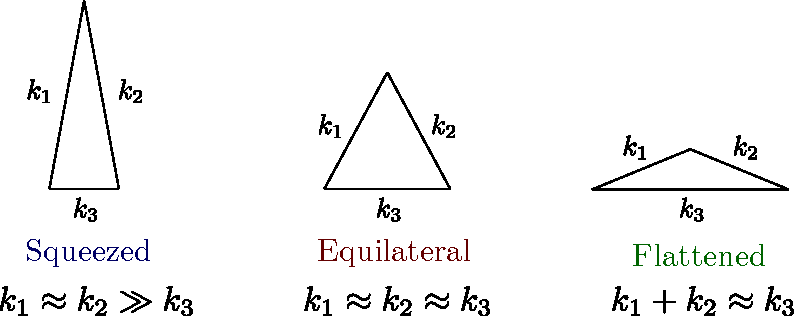
\includegraphics[width=0.8\textwidth]{triangle_configurations.pdf}
	\hspace{10pt}
	\caption{Three notable triangle configurations for the bispectrum $B(k_1,k_2,k_3)$.}
	\label{fig:triangle_configurations}
\end{figure}

The squeezed, equilateral and flattened limits of bispectra all have distinct physical meanings. For example, the squeezed limit corresponds to a configuration with two small-scale (large $k$) modes and one large-scale (small $k$) mode. Heuristically, this relates to how the small scale covariances are affected by an encompassing large-scale mode.

One of the most studied bispectrum shapes comes from the \textit{local} model. In this model, the perturbative field $\zeta(\vv{x})$ is expanded as a local function of some Gaussian field $\zeta_\text{G}(\vv{x})$ as
\begin{align}
	\zeta(\vv{x}) = \zeta_\text{G}(\vv{x}) + \frac{3}{5} f_\text{NL} \left(\zeta_\text{G}^2(\vv{x}) - \left< \zeta_\text{G}^2 \right> \right) + \cdots. \label{eqn:local_model_fNL_defitintion}
\end{align}
The non-linearity parameter $f_\text{NL}$ measures the amplitude of quadratic contributions to the field. A factor of $(3/5)$ here is conventional; the original definition of $f_\text{NL}$ was written in terms of the potential $\Phi$, which is equal to $(3/5)\zeta$ on super-horizon scales.

Substituting this form into \eqref{eqn:bispectrum_from_fourier_derivation_1} gives an expression involving correlation functions of four Gaussian fields, to leading order in $f_\text{NL}$. Isserlis' theorem, also known as Wick's theorem to physicists, allows us to write such four-point correlators in terms of the sum over all possible contractions:
\begin{align}
	\left< \zeta_\text{G}(\vv{x}_1)^2 \zeta_\text{G}(\vv{x}_2) \zeta_\text{G}(\vv{x}_3) \right> = &\left< \zeta_\text{G}(\vv{x}_1)^2 \right> \left< \zeta_\text{G}(\vv{x}_2) \zeta_\text{G}(\vv{x}_3) \right> + \left< \zeta_\text{G}(\vv{x}_1) \zeta_\text{G}(\vv{x}_2) \right> \left< \zeta_\text{G}(\vv{x}_1) \zeta_\text{G}(\vv{x}_3) \right> \nonumber \\ &\hspace{0.15\textwidth} + \left< \zeta_\text{G}(\vv{x}_1) \zeta_\text{G}(\vv{x}_3) \right> \left< \zeta_\text{G}(\vv{x}_1) \zeta_\text{G}(\vv{x}_2) \right>. \label{eqn:local_model_derivation_1}
\end{align}
Contributions from the first term in \eqref{eqn:local_model_derivation_1} cancel out with the ones coming from $\left< \zeta_\text{G}^2 \right>$ in the definition \eqref{eqn:local_model_fNL_defitintion}. After expressing the two-point correlations in terms of the power spectrum in Fourier space as $\left< \zeta_\text{G}(\vv{k}_1) \zeta_\text{G}(\vv{k}_2) \right> = (2\pi)^3 \delta^{(3)}(\vv{k}_1 + \vv{k}_2) P_\zeta (k_1, k_2)$, we obtain the \textit{local} bispectrum;
\begin{align}
	B(k_1, k_2, k_3) = \frac{3}{5} f_\text{NL} \left[ 2P_\zeta(k_2) P_\zeta(k_3) + 2P_\zeta(k_3) P_\zeta(k_1) + 2P_\zeta(k_1) P_\zeta(k_2) \right]. \label{eqn:local_bispectrum_using_power_spectrum}
\end{align}

Due to this fact, it is common in literature (e.g. \cite{Burrage2011large}) to define `the reduced bispectrum' $f_\text{NL}$ to be $f_\text{NL}(k_1,k_2,k_3) := 5B(k_1,k_2,k_3) / 6(P(k_1)P(k_2) + P(k_2)P(k_3) + P(k_3)P(k_1))$. $f_\text{NL}$ is then a three-dimensional function in general. This is potentially confusing because of a conflicting convention in the observational community where $f_\text{NL}$ represents a parameter measuring the amplitude of a specific bispectrum shape.

In this thesis, we follow the latter convention and associate one scalar $f_\text{NL}$ with each of the bispectrum shapes. For example, $f_\text{NL}$ in \eqref{eqn:local_bispectrum_using_power_spectrum} is denoted $f_\text{NL}^\textrm{local}$, tied to the local shape. The connection between the theoretical predictions and observations is often made using approximate analytic templates for the bispectrum.

We parametrise the power spectrum as $P_\zeta(k) = A_\zeta k^{n_s-4}$ using the power spectrum amplitude $A_\zeta$ and scalar spectral index $n_s$. The local bispectrum template is then defined as 
\begin{align}
	B_\zeta^\textrm{local} (k_1, k_2, k_3) := 2A^2 \left[ \frac{1}{k_1^{4-n_s} k_2^{4-n_s}} + \text{\;2 cyc.} \right], \label{def:local_template} 
\end{align}
where $A^2 := (3/5) A_\zeta^2$. Note that we do not include $f_\text{NL}^\textrm{local}$ in our definition of the template either; it is set to one.

The primordial bispectrum from multi-field inflation models typically falls into this category (reviewed in e.g., \cite{Byrnes2010review}). The local shape peaks in the squeezed limit where ${k_1 \approx k_2 \gg k_3}$, diverging as $k_3\rightarrow0$. General single-field models, on the other hand, are better described by the equilateral and orthogonal templates \cite{Creminelli2006limits,Senatore2010orthogonal}:
\begin{align}
	B_\zeta^\textrm{equil} (k_1, k_2, k_3) &:= 6A^2 \left[ -\left( \frac{1}{k_1^{4-n_s} k_2^{4-n_s}} + \text{2 cyc.} \right) -\frac{2}{(k_1 k_2 k_3)^{2(4-n_s)/3}} \right.\nonumber\\
	&\hspace{0.2\textwidth} + \left. \left( \frac{1}{k_1^{(4-n_s)/3} k_2^{2(4-n_s)/3} k_3^{(4-n_s)}} + \text{5 cyc.} \right) \right], \label{def:equilateral_template} \\
	B_\zeta^\textrm{ortho} (k_1, k_2, k_3) &:= 6A^2 \left[ -3\left( \frac{1}{k_1^{4-n_s} k_2^{4-n_s}} + \text{ 2 cyc.} \right) -\frac{8}{(k_1 k_2 k_3)^{2(4-n_s)/3}} \right.\nonumber\\
	&\hspace{0.2\textwidth} + \left. 3\left( \frac{1}{k_1^{(4-n_s)/3} k_2^{2(4-n_s)/3} k_3^{(4-n_s)}} + \text{5 cyc.} \right) \right]. \label{def:orthogonal_template} 
\end{align}
The equilateral and orthogonal shapes are peaked at the equilateral and flattened limits shown in Figure \ref{fig:triangle_configurations}, respectively. The latter was constructed explicitly to probe bispectrum shapes perpendicular to the equilateral shape.

\section{Primordial non-Gaussianity} \label{section:primordial_non_Gaussianity}

Previously in Section \ref{section:quantum_fluctuations}, we derived the power spectrum of perturbations in the inflation field assuming a homogeneous background. This section outlines how to compute cosmological correlation functions from single-field inflation in general.

We introduce the necessary tools in Section \ref{section:in_in_formalism} and \ref{section:ADM_formalism}. The bispectrum from a general type of single-field inflation is derived in Section \ref{section:bispectrum_from_single_field_inflation}. We focus on illustrating the framework without delving too much into the technical details. A simple example is used to demonstrate how explicit calculations are done, while we refer to, e.g., \cite{Maldacena2013,Chen2010review,Burrage2011large} for the full (and laborious) calculations.

\subsection{ADM formalism} \label{section:ADM_formalism}

In order to study the perturbed metric in the presence of one or more inflation fields, it is convenient to use the Arnowitt-Deser-Misner (ADM) formalism \cite{Arnowitt2008ADMrepublication}:
\begin{align}
	ds^2 = -N dt^2 + h_{ij}(dx^i + N^i dt) (dx^j + N^j dt),
\end{align}
where the lapse and shift functions $N$ and $N^i$, respectively, are non-dynamical variables of the action. They act as Lagrange multipliers and provide constraint equations. We focus on the scalar perturbations here and ignore vector and tensor modes since they evolve independently owing to the SVT theorem. The spatial metric $h_{ij}$ contains two scalar degrees of freedom. When inflation is driven by a single scalar field, there is one extra scalar mode from perturbations of the field. Out of the three dynamical scalar degrees of freedom, two can be fixed by a gauge choice as we saw in \ref{section:metric_perturbations}. Here we choose the gauge so that the inflation field is uniform. The spatial metric takes the form
\begin{align}
	h_{ij} = a(t)^2 \;e^{2\zeta} \; \delta_{ij},  \label{eqn:spatial_metric_curvature_perturbation}
\end{align}
where $\zeta(\vv{x},t)$ is equivalent to the curvature perturbation we defined earlier in \eqref{def:curvature_perturbation}. Note that, if we define $N(t) = \int^{t}_{t_0} H dt' = \ln a(t) - \ln a(t_0)$ (not to be confused with the lapse function $N$) to represent the number of $e$-folds of expansion between time $t$ and $t_0$, then $\zeta = \delta N$. \footnote{To be precise, $\delta N$ is defined as in \eqref{eqn:local_clock_time_fluctuation} with $f=N$. We have $\zeta(t,\vv{x})= \delta N = N(t+\delta t) - N(t)$, where $\delta t(t,\vv{x})$ represents the perturbations in the inflationary `clock time' at the given spatial position $\vv{x}$.}
	
We now write down the action. Compared to \eqref{eqn:real_scalar_field_action}, the Einstein-Hilbert term is added since the metric is no longer fixed. We consider a generalised form of the field Lagrangian with the action given by
\begin{align}
	S = \int dt d^3 \vv{x} \; \sqrt{-g} \left[ \frac{M_\textrm{p}}{2} R + P(X,\phi) \right],  \label{eqn:general_single_field_action}
\end{align}
where $M_\textrm{p} := (8\pi G)^{-1/2}$ is the reduced Planck mass and $X:=-\frac{1}{2} g^{\mu\nu} \partial_\mu \phi \partial_\nu \phi$ is the canonical kinetic term. We set $M_\textrm{p}=1$ for convenience. $P(X,\phi)$ is an arbitrary function which generalises $X-V(\phi)$ of the standard slow-roll inflation \cite{Chen2007b}.

One notable consequence of the non-trivial kinetic term $P$ is that the fluctuations in the inflation field no longer necessarily propagate with the speed of light. The sound speed, defined as the ratio $\delta P / \delta \rho$, in these models is given by
\begin{align}
	c_\text{s}^2 = \frac{P_{,X}}{P_{,X} + 2 X P_{,XX}}, \label{eqn:general_single_field_sound_speed}
\end{align}
where the subscript `$,X$' represents taking a partial derivative with respect to $X$.

In the ADM formalism, \eqref{eqn:general_single_field_action} becomes
\begin{align}
	S = \frac{1}{2}\int dt d^3 \vv{x} \; \sqrt{h} \; N \left[ R^{(3)} + 2P(X,\phi) \right] + \frac{1}{2} \int dt d^3 \vv{x} \; \sqrt{h} \; N^{-1} \left[ E_{ij} E^{ij} - E^2 \right],
\end{align}
where the $R^{(3)}$ is the three-dimensional Ricci scalar of $h_{ij}$, and
\begin{align}
	E_{ij} := \frac{1}{2} \left( \dot{h}_{ij} - \nabla_i N_j - \nabla_j N_i \right), \hspace{0.05\textwidth}
	E := E_{ij} h^{ij}.
\end{align}
The spatial indices $i,j$ are lowered and raised by $h_{ij}$.

In order to obtain an action for $\zeta$, we substitute \eqref{eqn:spatial_metric_curvature_perturbation} into the expression and expand perturbatively in $\zeta$. We keep terms of order up to three as they are all that is relevant for three-point correlation functions. It is sufficient to evaluate $N$ and $N_i$ to first order in $\zeta$ since they multiply with constraint equations which vanish up to first order.

The quadratic part of the action is given by
\begin{align}
	S_2 = \int dt d^3\vv{x} \; \left[ \frac{\epsilon}{c_\text{s}^2} a^3 \dot{\zeta}^2 - \epsilon a(\partial\zeta)^2  \right], \label{eqn:quadratic_action_in_zeta}
\end{align}
where the slow-roll parameter $\epsilon=-\dot{H}/H^2$ has made a reappearance. Here, $(\partial\zeta)^2$ is shorthand for $\partial_i \zeta \partial^i \zeta$ which involves the spatial derivatives of $\zeta$. Note that there are no terms proportional to $\zeta^2$ in the quadratic action, meaning that $\zeta$ is massless even without the slow-roll assumptions.

The third order action contains many terms with varying amounts of contributions to the bispectrum. We write only one particular term here for an example calculation which will be shown later. The full result can be found in \cite{Chen2007b}. 
\begin{align}
	S_3 \supset \int d\tau d^3\vv{x} \; a^3 \left[ -\frac{\epsilon}{H c_\text{s}^2} \left( 1 - \frac{1}{c_\text{s}^2} \right) + \frac{2\lambda c_\text{s}^2}{H^2 \epsilon} \right] \dot{\zeta}^3.	 \label{eqn:cubic_action_example_term}
\end{align}

\subsection{In-in formalism} \label{section:in_in_formalism}

We need to calculate the Hamiltonian from the action in order to quantise the field. When only the quadratic part \eqref{eqn:quadratic_action_in_zeta} is considered, the corresponding Hamiltonian, say $H_0$, is also quadratic in $\zeta$ and its conjugate momentum $\pi := \partial\Lagr/\partial(\dot{\zeta})$. $H_0$ describes the free theory in which the equations of motion are linear and we can find the mode functions that solve them, as we did in Section \ref{section:quantum_fluctuations}. Meanwhile, third-order and higher terms in the action such as \eqref{eqn:cubic_action_example_term} appear in the Hamiltonian as couplings that contribute to the correlation functions. Denoting these `interacting' terms as $H_\text{int}$, the total Hamiltonian for the perturbations takes the form
\begin{align}
	H = H_0 + H_\text{int}. \label{eqn:interaction_picture_hamiltonian}
\end{align}

There are multiple formalisms in quantum mechanics regarding the time evolution of operators and states. In the Schr\"odinger picture, the states evolve in time according to the Hamiltonian, while the operators remain fixed over time. On the other hand, the Heisenberg picture has the operators varying in time and the states constant. Yet another alternative is the interaction picture where the Hamiltonian \eqref{eqn:interaction_picture_hamiltonian} is split into two parts, responsible for the time evolution of the states and the operators, respectively. All three pictures are physically equivalent; all the correlation function values are identical between them.

We choose to work in the interaction picture where the operators and states evolve in time through $H_0$ and $H_\text{int}$, respectively. The main advantage of this formalism is that we can use the results from the free ($H=H_0$) theory to evolve operators in time. In particular, we may canonically quantise the field $\hat{\zeta}(\vv{x},t)$ using its Fourier transform;
\begin{align}
	\hat{\zeta}_\vv{k} (t) = u_k(t) \; \hat{a}_\vv{k} + u_k^*(t) \; \hat{a}_{-\vv{k}}^\dagger, \label{eqn:zeta_canonical_quantisation}
\end{align} 
where the mode functions $u_k(\tau)$ satisfy the equations of motion from the quadratic action \eqref{eqn:quadratic_action_in_zeta} related to $H_0$, which we can solve analytically. Note that $u_k(\tau)$ depends only on $k=\|\vv{k}\|$ because the spatial derivatives enter through $(\partial\zeta)^2$ only. The annihilation and creation operators $\hat{a}_\vv{k}$ and $\hat{a}_{-\vv{k}}^\dagger$ satisfy the usual commutation relations: ${[\hat{a}_{\vv{k}_1},\hat{a}_{\vv{k}_2}^\dagger] = (2\pi)^3 \delta^{(3)}(\vv{k}_1-\vv{k}_2)}$.

Meanwhile, all the information about the interactions is captured in the time evolution operator $\hat{U_I}(t,t_0) = T\exp \left(-i\int_{t_0}^t H_\text{I}(t')dt'\right)$, where $H_\text{I}$ denotes $H_\text{int}$ in the interaction picture. The time-ordering operator $T$ arranges the operators so that the ones evaluated at earlier times appear on the right. The states at time $t$ are given by $|\psi_I(t)\rangle = U_I(t,t_0) |\psi_I(t_0)\rangle$.

The in-in formalism (\cite{Schwinger1961inin,Jordan1986inincosmo1,Calzetta1987inincosmo2}) allows us to calculate correlation functions at a given time $t$ using two `in' states: two copies of the vacuum at infinite past in our case. For some local operator $Q(t)$ written as a product of $\hat{\zeta}(\vv{x},t)$ and $\hat{\pi}(\vv{x},t)$, we define its expected value as follows;
\begin{align}
	\left< Q(t) \right> &:= \langle \textrm{in} |\;Q(t)\;| \textrm{in} \rangle \nonumber\\ &=  \langle\vv{0}| \left[ \bar{T} \exp \left( i \int_{t_0}^{t} H_\text{I}(t')dt \right) \right] Q_I(t) \left[ T \exp \left( -i \int_{t_0}^{t} H_\text{I}(t')dt \right) \right]  |\vv{0}\rangle. \label{eqn:in_in_formalism_expectation}
\end{align}
The interaction picture vacuum, $|\vv{0}\rangle$, lies in the infinite past $t=t_0$, where we assume that it can be identified as the vacuum of non-interacting theory and hence $a_\vv{k}|\vv{0}\rangle = 0$.

Note that the operators within the correlator in \eqref{eqn:in_in_formalism_expectation} are not time-ordered thanks to the anti-time-ordering operator $\bar{T}$. To complicate things further, we do not have an equivalent of the Feynmann propagator in Minkowski space that handles the time ordering for us. We instead treat the time ordering manually. Let us define the \textit{contraction} between two terms $\zeta(\vv{k}_1,t_1)$ on the left and $\zeta(\vv{k}_2,t_2)$ on the right as the commutator given by
\begin{align}
	[ \zeta^+(\vv{k}_1,t_1) , \zeta^-(\vv{k}_2,t_2) ] &= u_{k_1}(t_1) u^*_{k_2}(t_2) [ \hat{a}_{\vv{k_1}}, \hat{a}_{\vv{k_2}}^\dagger] \\ &= u_{k_1}(t_1) u^*_{k_2}(t_2) (2\pi)^3 \delta^{(3)} (\vv{k}_1 + \vv{k}_2), 
\end{align}
where the positive and negative frequency solutions $\zeta^+$ and $\zeta^-$ refer to the terms with $\hat{a}$ and $\hat{a}^\dagger$ in \eqref{eqn:zeta_canonical_quantisation}, respectively. Note that swapping the order of $\zeta(\vv{k}_1,t_1)$ and $\zeta(\vv{k}_2,t_2)$ does alter the value of this commutator. We make equivalent definitions for the quantised conjugate momenta $\hat{\pi}_\vv{k}$.

We now have a result comparable to Wick's theorem;
\begin{align}
	\langle\vv{0}| \hat{O}(\vv{k}_1,t_2) \cdots \hat{O}(\vv{k}_n,t_n) |\vv{0}\rangle = \;:\; \hat{O}(\vv{k}_1,t_2)  \cdots \hat{O}(\vv{k}_n,t_n) \;:\; + \;:\;\text{all possible contractions}\;:\;. \label{eqn:in_in_Wicks_theorem}
\end{align}
The normal ordering $::$ keeps $\hat{a}$s to the right and $\hat{a}^\dagger$ to the left so that the vacuum expectation value vanishes. The fields $\hat{O}$ are either $\hat{\zeta}$ or $\hat{\pi}$. 

\subsection{Bispectrum from single-field inflation} \label{section:bispectrum_from_single_field_inflation}

The mode function defined in \eqref{eqn:zeta_canonical_quantisation} can be obtained analytically by solving the equations of motion from the quadratic action \eqref{eqn:quadratic_action_in_zeta}. If the slow-roll and other variation parameters remain small and change slowly in time, then
\begin{align}
	u_k(\tau) = \frac{iH}{\sqrt{4\epsilon c_\text{s} k^3}} (1 + ikc_\text{s} \tau) e^{-ikc_\text{s} \tau},
\end{align}
where $\tau$ is conformal time. The choice of $u_k(\tau)$ being the positive frequency solution as shown here is analogous to \eqref{eqn:bunch_davies_mode_function} from before; we are fixing the vacuum state to be the Bunch-Davies vacuum.

Before proceeding to compute correlation functions using the in-in formalism, we first need to obtain the Hamiltonian of the system. The conjugate momentum is defined as $\pi = \partial \mathcal{L} / \partial \dot{\zeta}$, where $\mathcal{L}$ is the Lagrangian density. The Hamiltonian density then takes the form $\mathcal{H} = \pi \dot{\zeta} - \mathcal{L} = \mathcal{H}_0 + \mathcal{H}_\text{int}$. At the order of perturbations we are studying, $\mathcal{H}_\text{int}$ consists only of cubic terms $\mathcal{H}_3$, which is simply equal to $-\mathcal{L}_3$ obtained from the cubic action $S_3$. It is also sufficient to consider the leading contribution to $\zeta$, so that $\pi \propto \dot{\zeta}$.
\footnote{There are some subtleties here. We first use $\pi = \partial \mathcal{L} / \partial \dot{\zeta}$, which does contain contributions from higher order terms coming from $\mathcal{L}=\mathcal{L}_0 + \mathcal{L}_{int}$. The Hamiltonian density $\mathcal{H} = \pi \dot{\zeta} - \mathcal{L}$ is obtained using this $\pi$. We then rewrite $\pi$ in terms of $\zeta$ and its derivatives within $\mathcal{H}$. Next, the quadratic terms in $\mathcal{H}$ are combined as $\mathcal{H}_0$. From this free Hamiltonian we define the conjugate momentum in the interaction picture; $\pi_I :=  \partial \mathcal{H}_0 / \partial \dot{\zeta}$. This $\pi_I$ is what we refer to as $\pi$, simply proportional to $\dot{\zeta}$ in our case.}
We will rewrite $\pi$ in terms of $\dot{\zeta}$ the rest of this section.

When working perturbatively, the leading contributions to the three-point correlation function comes from the terms with one factor of the interaction Hamiltonian. Noting that the two terms coming from the two $H_\text{I}$s in \eqref{eqn:in_in_formalism_expectation} are complex conjugates to each other, we have
\begin{align}
	\left< \zeta_{\vv{k}_1}(t) \zeta_{\vv{k}_2}(t) \zeta_{\vv{k}_3}(t) \right> = 2 \text{Re}\left[ \langle\vv{0}| -i \zeta_{\vv{k}_1}(t) \zeta_{\vv{k}_2}(t) \zeta_{\vv{k}_3}(t) \int_{t_0}^{t} H_\text{I}(t') dt' |\vv{0}\rangle \right], \label{eqn:in_in_formalism_bispectrum}
\end{align}
in tree-level. This is the key formula for computing the primordial bispectrum from a given single-field inflation Lagrangian.

We will now demonstrate how to compute \eqref{eqn:in_in_formalism_bispectrum} using a simple example. We take the term proportional to $\dot\zeta^3$ within the cubic action \eqref{eqn:cubic_action_example_term}. To simplify further, we write it as $\mu a^3 \dot{\zeta}^3$, where $\mu=\mu(t)$ is given in terms of the variation parameters such as $\lambda$ and $\epsilon$. The corresponding contribution to the interaction Hamiltonian is given by
\begin{align}
	H_{\text{I},\dot{\zeta}^3}(t) &:= -\mu(t) a(t)^3 \int d^3\vv{x} \; \left[  \dot{\zeta}(\vv{x},t)^3 \right]  \\
	&= -\mu a^3 \int d^3\vv{x} \; \frac{d^3\vv{p}_1}{(2\pi)^3} \frac{d^3\vv{p}_2}{(2\pi)^3} \frac{d^3\vv{p}_3}{(2\pi)^3} \; e^{i(\vv{p}_1 + \vv{p}_2 + \vv{p}_3)\cdot\vv{x}} \left[ \dot{\zeta}_{\vv{p}_1} \dot{\zeta}_{\vv{p}_2} \dot{\zeta}_{\vv{p}_3} \right] \\
	&= - (2\pi)^3 \delta^{(3)}(\vv{p}_1 + \vv{p}_2 + \vv{p}_3) \cdot \mu a^3 \int \frac{d^3\vv{p}_1}{(2\pi)^3} \frac{d^3\vv{p}_2}{(2\pi)^3} \frac{d^3\vv{p}_3}{(2\pi)^3} \; \left[ \dot{\zeta}_{\vv{p}_1} \dot{\zeta}_{\vv{p}_2} \dot{\zeta}_{\vv{p}_3} \right], \label{def:interaction_hamiltonian_zeta_dot_cube}
\end{align}
where we used the definition of Fourier transformation and omitted the time dependence for brevity. Note also that $\zeta_{\vv{p}}(t) = const$ after the mode crosses the horizon because the curvature perturbation freezes out at super-horizon scales\textemdash a result we have shown in Section \ref{section:curvature_perturbations}.

We substitute \eqref{def:interaction_hamiltonian_zeta_dot_cube} into \eqref{eqn:in_in_formalism_bispectrum} and swap the order of expectations and integrals. The integrand include a six-point correlation function which can be evaluated using \eqref{eqn:in_in_Wicks_theorem};
\begin{align}
	&\langle\vv{0}| \zeta_{\vv{k}_1}(t) \zeta_{\vv{k}_2}(t) \zeta_{\vv{k}_3}(t) \zeta_{\vv{p}_1}(t') \zeta_{\vv{p}_2}(t') \zeta_{\vv{p}_3}(t') |\vv{0}\rangle \nonumber\\
	&\hspace{0.05\textwidth}= \langle\vv{0}| \;: \text{all contractions} :\;|\vv{0}\rangle \\
	&\hspace{0.05\textwidth}= [ \zeta^+(\vv{k}_1,t) , \zeta^-(\vv{p}_1,t') ] [ \zeta^+(\vv{k}_2,t) , \zeta^-(\vv{p}_2,t') ] [ \zeta^+(\vv{k}_3,t) , \zeta^-(\vv{p}_3,t') ] + \text{5 perms.}  \\
	&\hspace{0.05\textwidth}=  \prod_{j=1}^{3} \left[ u_{k_j} \dot{u}^*_{p_j}(t') (2\pi)^3 \delta^{(3)}(\vv{k}_j+\vv{p}_j) \right] + \text{5 perms.}.
\end{align}
Note that we discarded some terms which involve contracting the fields at equal times. Such contractions necessarily cause one of the $\vv{p}_j$ to be $\vv{0}$ due to the delta function present in \eqref{def:interaction_hamiltonian_zeta_dot_cube}. $\zeta_\vv{0}$ corresponds to a constant scaling of the background $a(t)$, and after absorbing that factor into $a(t)$, $\zeta_{\vv{0}}$ can be set to zero. 

Combining the results so far, we obtain the following expression for the bispectrum induced by the $\dot{\zeta}^3$ term
\begin{align}
	B_{\dot{\zeta}^3}(k_1,k_2,k_3,t) = \text{Re}\left[ 2i u_{k_1}(t) u_{k_2}(t) u_{k_3}(t) \int_{t_0}^{t} dt' \mu(t') a(t')^3 \dot{u}^*_{k_1}(t') \dot{u}^*_{k_2}(t') \dot{u}^*_{k_3}(t')   + \text{5 perms} \right].
\end{align}
In order to evaluate the bispectrum at the end of inflation, we convert back from comoving to conformal time. The time integral is then taken from $\tau=-\infty$ to $\tau=0$. The lower limit of the integral can be troublesome since $e^{i k c_\text{s} \tau}$ in the mode function displays oscillatory behaviour as $\tau\rightarrow -\infty$. We shift $-\infty$ to $-\infty(1+i\epsilon)$ so that the integrand is suppressed at the lower limit. We further approximate the variation parameters including $\mu(\tau)$ to be constant and use the de Sitter background $a(\tau)\approx -1/(H\tau)$ within the integral;
\begin{align}
	B_{\dot{\zeta}^3}(k_1,k_2,k_3) &\approx -12\mu \cdot \text{Imag}\left[  u_{k_1}(0) u_{k_2}(0) u_{k_3}(0) \int_{-\infty(1+i\epsilon)}^{0} d\tau \;  a(\tau) {u'}^*_{k_1}(\tau) {u'}^*_{k_2}(\tau) {u'}^*_{k_3}(\tau)  \right] \\
	&= -12\mu \cdot \text{Imag} \left[ \frac{H^5 c_\text{s}^3}{64\epsilon^3} \frac{1}{k_1 k_2 k_3} \int_{-\infty(1+i\epsilon)}^{0} d\tau \; \tau^2 e^{ic_\text{s}\tau(k_1+k_2+k_3)} \right] \\
	&= \frac{3\mu H^5}{8\epsilon^3} \frac{1}{k_1 k_2 k_3} \frac{1}{(k_1+k_2+k_3)^3}.
\end{align}
The corresponding shape function takes the form
\begin{align}
	S_{\dot{\zeta}^3}(k_1,k_2,k_3) \propto \frac{k_1 k_2 k_3}{(k_1+k_2+k_3)^3},
\end{align}
which is maximised in the equilateral limit and vanishes at the squeezed limit.

The full bispectrum can be computed using the general methodology shown in this section. We quote one of the most important results; for canonical slow-roll inflation with $P(X,\phi) = X - V(\phi)$, the bispectrum is suppressed by the slow-roll parameters $\epsilon$ and $\eta$ \cite{Maldacena2013}. However, relaxing any of the assumptions\textemdash canonical kinetic term, slow-roll, single-field, and Bunch-Davies vacuum\textemdash may yield significant and observable signatures in the bispectrum (see \cite{Chen2010review,Komatsu2010} for reviews).

\section{CMB bispectrum estimation} \label{section:CMB_bispectrum_estimation}

The presence of a non-vanishing bispectrum at the end of inflation due to primordial non-Gaussianity leaves imprints on the CMB. The bispectrum of the observed CMB anisotropy directly relates to the primordial counterpart thanks to the linear nature of the evolution and hence is a key statistic for constraining primordial non-Gaussianity.

The CMB appears consistent with being Gaussian distributed, so its bispectrum has relatively small signal-to-noise. In contrast to the power spectrum analysis where we treat each $C_l$ (after binning) as an independent data point, the noise-dominated $b_{l_1 l_2 l_3}$s are not so significant individually. Therefore, we instead fit the whole bispectrum data to the theoretical prediction from a given model in order to estimate a single parameter measuring the amplitude: $f_\text{NL}$.

In this section, we formulate the theory of CMB bispectrum estimation. Estimating $f_\text{NL}$ is an extremely challenging task due to its computational complexity and the oscillatory integrals involved. We review several conventional approaches to handle these challenges and summarise their respective strengths and weaknesses. Lastly, we discuss some significant non-primordial sources of non-Gaussianity that needs to be carefully accounted for in the estimation process.


\subsection{CMB bispectrum}

Consider the three-point correlation function of the spherical harmonic coefficients $a_{lm}^X$ from \eqref{eqn:alm_from_phi};
\begin{align}
	\left< a_{l_1 m_1}^{X_1} a_{l_2 m_2}^{X_2} a_{l_3 m_3}^{X_3}  \right> = (4\pi)^3 (-i)^{l_1 + l_2 + l_3} \left< \prod_{j=1}^{3} \left[ \int \frac{d^3\vv{k}_j}{(2\pi)^3} \zeta(\vv{k}_j)   \Delta_{l_j}^{X_j} (k_j) Y^*_{l_j m_j} (\hat{\vv{k}}_j) \right] \right>, \label{eqn:bispectrum_derivation_base_form}
\end{align}
where we replaced $\Phi$ with $\zeta$ in the integrand. Here, $X_j$s can be either $T$ or $E$ which correspond to the temperature and E-mode polarisation of the CMB anisotropy, respectively. The transfer functions $\Delta_l^X (k)$ for $\zeta$ depend only on $k=\left\| \vv{k} \right\|$. They incorporate all information about the evolution of the primordial perturbations $\zeta$ and then projection onto the observed sky today.

We may take everything but $\zeta(\vv{k_j})$s outside the brackets $\left< \cdot \right>$. From the definition of bispectrum, we have
\begin{align}
	\left< \zeta(\vv{k}_1) \zeta(\vv{k}_2)  \zeta(\vv{k}_3) \right> &= (2\pi)^3 \delta^{(3)}(\vv{k}_1 + \vv{k}_2 + \vv{k}_3) B(k_1, k_2, k_3) \label{eqn:primordial_bispectrum}\\
	&= \int d^3 \vv{r} \; e^{-i\vv{r} \cdot (\vv{k}_1 + \vv{k}_2 + \vv{k}_3)}  B(k_1, k_2, k_3), \label{eqn:bispectrum_derivation_delta_function}
\end{align}
where an integral expression is substituted for the Dirac $\delta$-function in the second line. At the cost of introducing an extra integral, we managed to express the $\delta$-function in a separable form: $\exp(\vv{r} \cdot (\vv{k}_1+\vv{k}_2+\vv{k}_3)) = \exp(\vv{r}\cdot \vv{k}_1) \exp(\vv{r}\cdot \vv{k}_2) \exp(\vv{r}\cdot \vv{k}_3)$. The remaining exponentials are rewritten using the plane wave expansion;
\begin{align}
	e^{-i \vv{k} \cdot \vv{r}} &= \sum_{l=0}^{\infty} (2l+1) (-i)^l j_l(kr) P_l(\hat{\vv{k}} \cdot \hat{\vv{r}})  \\	
	&= \sum_{l=0}^{\infty} \sum_{m=-l}^{l} 4\pi (-i)^l j_l(kr) Y_{lm}(\hat{\vv{k}}) Y^*_{lm}(\hat{\vv{r}}). \label{eqn:bispectrum_derivation_rayleigh}
\end{align}
The Legendre polynomial $P_l(\hat{\vv{k}} \cdot \hat{\vv{r}})$ has been expanded using the spherical harmonic addition theorem in the last line. Note that $\vv{k}$ and $\vv{r}$ mix only through their amplitudes within the spherical bessel functions as $j_l(kr)$. Once substituted into (\ref{eqn:bispectrum_derivation_base_form}), we can perform the angular integral $d^2 \hat{\vv{k}_j}$ separately for each $j=1,2,3$, since $d^3\vv{k}_j = dk_j k_j^2 d^2 \hat{\vv{k}_j}$. Note also that the spherical harmonic orthogonality relation is given by
\begin{align}
	\int d^2 \hat{\vv{n}} \; Y_{lm}(\hat{\vv{n}}) Y^*_{l'm'}(\hat{\vv{n}}) = \delta_{l l'} \delta_{m m'}.
\end{align}
There are no implied summations over indices throughout this section. Incorporating \eqref{eqn:bispectrum_derivation_base_form}, \eqref{eqn:bispectrum_derivation_delta_function}, and \eqref{eqn:bispectrum_derivation_rayleigh}, we obtain
\begin{align}
	&\left< a_{l_1 m_1}^{X_1} a_{l_2 m_2}^{X_2} a_{l_3 m_3}^{X_3}  \right> \nonumber \\
	&\hspace{0.05\textwidth}= \frac{(4\pi)^3}{(2\pi)^9} (-1)^{l_1 + l_2 + l_3} \int d^3 \vv{r} \; d^3 \vv{k}_1 d^3 \vv{k}_2 d^3 \vv{k}_3 \; B(k_1,k_2,k_3) \nonumber \\
	&\hspace{0.25\textwidth} \times \prod_{j=1}^{3} \left[ \sum_{l'_j = 0}^{\infty} \sum_{m'_j=-l'_j}^{l'_j} j_{l'_j} (k_j r) Y_{l'_j m'_j} (\hat{\vv{k}}_j) Y^*_{l'_j m'_j} (\hat{\vv{r}}) \Delta_{l_j}^{X_j} (k_j) Y^*_{l_j m_j} (\hat{\vv{k}}_j) \right]  \label{eqn:bispectrum_derivation_main_line1}\\
	&\hspace{0.05\textwidth}= \left( \frac{2}{\pi} \right)^3 \int d^3 \vv{r} \; dk_1 dk_2 dk_3 \left( k_1 k_2 k_3 \right)^2 B(k_1, k_2, k_3) \prod_{j=1}^{3} \left[ j_{l_j} (k_j r) Y^*_{l_j m_j} (\hat{\vv{r}}) \Delta_{l_j}^{X_j} (k_j) \right]  \label{eqn:bispectrum_derivation_main_line2}\\
	&\hspace{0.05\textwidth}= \left( \frac{2}{\pi} \right)^3 \mathcal{G}^{l_1 l_2 l_3 *}_{m_1 m_2 m_3} \int dr \; dk_1 dk_2 dk_3 r^2 \left( k_1 k_2 k_3 \right)^2 B(k_1, k_2, k_3) \prod_{j=1}^{3} \left[ j_{l_j} (k_j r) \Delta_{l_j}^{X_j} (k_j) \right], \label{eqn:bispectrum_derivation_main_line3}
\end{align}
where the Gaunt integral is defined as
\begin{align}
	\mathcal{G}^{l_1 l_2 l_3}_{m_1 m_2 m_3} := \int d^2 \hat{\vv{n}} \; Y_{l_1 m_1} (\hat{\vv{n}}) Y_{l_2 m_2} (\hat{\vv{n}}) Y_{l_3 m_3} (\hat{\vv{n}}). \label{def:gaunt_integral}
\end{align}
This value is always real, so we may omit the complex conjugate in (\ref{eqn:bispectrum_derivation_main_line3}). Note also that we dropped a factor of $(-1)^{l_1+l_2+l_3}$ in (\ref{eqn:bispectrum_derivation_main_line2}). This is due to parity reasons. Spherical harmonics have definite parity; $Y_{lm}(-\hat{\vv{n}}) = (-1)^l Y_{lm}(\hat{\vv{n}})$. Applying parity transformation to the integral in (\ref{def:gaunt_integral}) gives $\mathcal{G}^{l_1 l_2 l_3}_{m_1 m_2 m_3} = (-1)^{l_1+l_2+l_3} \mathcal{G}^{l_1 l_2 l_3}_{m_1 m_2 m_3}$. The Gaunt integral therefore evaluates to zero unless $l_1+l_2+l_3$ is even.

We define the \textit{reduced} bispectrum as
\begin{align}
	b^{X_1 X_2 X_3}_{l_1 l_2 l_3} := \left( \frac{2}{\pi} \right)^3 \int dr dk_1 dk_2 dk_3 \left(r k_1 k_2 k_3 \right)^2 B(k_1, k_2, k_3) \prod_{j=1}^{3} \left[ j_{l_j} (k_j r) \Delta_{l_j}^{X_j} (k_j) \right]. \label{def:reduced_bispectrum}
\end{align}
The late-time bispectrum can now be written in a concise form;
\begin{align}
	\left< a_{l_1 m_1}^{X_1} a_{l_2 m_2}^{X_2} a_{l_3 m_3}^{X_3}  \right> = \mathcal{G}^{l_1 l_2 l_3}_{m_1 m_2 m_3} b^{X_1 X_2 X_3}_{l_1 l_2 l_3}. \label{eqn:late_time_bispectrum_form}
\end{align}

Recall that the three-point function in (\ref{eqn:primordial_bispectrum}) is given by a product of delta function enforcing $\vv{k}_1 + \vv{k}_2 + \vv{k}_3 = \vv{0}$ and the primordial bispectrum $B(k_1,k_2,k_3)$. Its spherical harmonic counterpart (\ref{eqn:late_time_bispectrum_form}) takes an analogous form. The Gaunt integral $\mathcal{G}^{l_1 l_2 l_3}_{m_1 m_2 m_3}$ contains all geometrical information, enforcing the triangle condition on $l_1$, $l_2$, $l_3$ and angular momentum conservation $m_1+m_2+m_3=0$. Meanwhile, the reduced bispectrum encodes statistical information about the underlying three-point functions, just like $B(k_1,k_2,k_3)$.

The value of the Gaunt integral is best represented using Wigner 3-j symbols;
\begin{align}
	\mathcal{G}^{l_1 l_2 l_3}_{m_1 m_2 m_3} = \sqrt{\frac{(2l_1+1)(2l_2+1)(2l_3+1)}{4\pi}} \begin{pmatrix}	l_1 & l_2 & l_3 \\ m_1 & m_2 & m_3 \end{pmatrix} \begin{pmatrix}	l_1 & l_2 & l_3 \\ 0 & 0 & 0 \end{pmatrix}.
\end{align}
The Wigner 3-j symbols, written here as a 2-by-3 matrix, are closely related to the addition of angular momenta. They are real coefficients appearing in the expansion of the zero-total-angular-momentum state $|0 \; 0\rangle$;
\begin{align}
	| 0 \; 0 \rangle = \sum_{l_1,m_1} \sum_{l_2,m_2} \sum_{l_3,m_3} \begin{pmatrix}	l_1 & l_2 & l_3 \\ m_1 & m_2 & m_3 \end{pmatrix} | l_1 m_1 \rangle | l_2 m_2 \rangle | l_3 m_3 \rangle.
\end{align}
For further details on Wigner 3-j symbols see, e.g., \cite{Olver2010nist}. We quote the following two identities for our purposes.
\begin{align}
	\sum_{m_1,m_2,m_3} { \begin{pmatrix}	l_1 & l_2 & l_3 \\ m_1 & m_2 & m_3 \end{pmatrix} }^2 &= 1, \label{eqn:wigner_3j_normalisation} \\
	{ \begin{pmatrix}	l_1 & l_2 & l_3 \\ 0 & 0 & 0 \end{pmatrix} }^2 &= \frac{1}{2} \int_{-1}^{1} d\mu \; P_{l_1}(\mu) P_{l_2}(\mu) P_{l_3}(\mu). \label{eqn:wigner_3j_legendre_integral} 
\end{align}
The normalisation condition (\ref{eqn:wigner_3j_normalisation}) can be easily derived by computing the norm of the state $|0 \; 0 \rangle$ in the definition. The second identity (\ref{eqn:wigner_3j_legendre_integral}) allows us to rewrite a square of any given 3-j symbol satisfying $m_1=m_2=m_3=0$ in terms of a separable integral.

We make one last definition which will prove to be useful in the next section;
\begin{align}
	h^2_{l_1 l_2 l_3} :=& \sum_{m_1, m_2, m_3} \left( \mathcal{G}^{l_1 l_2 l_3}_{m_1 m_2 m_3} \right)^2  \label{def:h2_using_gaunt_integral}\\
	=& \frac{(2l_1+1)(2l_2+1)(2l_3+1)}{4\pi} { \begin{pmatrix}	l_1 & l_2 & l_3 \\ 0 & 0 & 0 \end{pmatrix} }^2 \\
	=& \frac{(2l_1+1)(2l_2+1)(2l_3+1)}{8\pi} \int_{-1}^{1} d\mu \; P_{l_1}(\mu) P_{l_2}(\mu) P_{l_3}(\mu). \label{def:h2_using_legendre_integral}
\end{align}

By squaring the Gaunt integral and summing over $m$s, we get a simpler quantity $h^2_{l_1 l_2 l_3}$ which preserves all of the important geometrical information. Here $l_1$, $l_2$ and $l_3$ must still satisfy triangle inequalities and add up to an even number. Otherwise, the integral over Legendre polynomials in (\ref{def:h2_using_legendre_integral}) vanishes.

\subsection{Optimal estimator}
The bispectrum of the CMB anisotropy is a powerful statistic for studying primordial non-Gaussianity. The Planck collaboration's CMB bispectrum analyses provided the most stringent bounds on the amplitude of primordial bispectrum with respect to various shapes and constrained a wide class of inflationary models. Due to the largely linear evolution of the CMB, there are few contributions to the bispectrum from non-primordial origins compared to other probes such as the large scale structure. Here, we derive the optimal CMB bispectrum estimator using mathematical foundations laid out previously.

Consider a number of inflation models which predict non-zero primordial bispectra. We often use template bispectra which capture some common characteristics of a class of models, like the local, equilateral, and orthogonal shapes (\ref{def:local_template}-\ref{def:orthogonal_template}). We would like to find out if the true underlying bispectrum, if any, can be expanded in terms of the functions $B^{(i)}$ chosen;
\begin{align}
	B(k_1,k_2,k_3) = \sum_i f_\text{NL}^{(i)} \; B^{(i)}(k_1,k_2,k_3), \label{eqn:primordial_bispectrum_fNLs}
\end{align}
where the primordial non-Gaussianity (or non-linearity) parameter $f^{(i)}_\text{NL}$ measures the magnitude of the $i$th bispectrum shape found in reality. Detection of a non-zero $f_\text{NL}$ would serve as strong evidence for the corresponding inflation models. Non-detection of $f_\text{NL}$, on the other hand, still allows us to place bounds on it and hence constrain models which predict larger bispectra.

Expressing (\ref{eqn:primordial_bispectrum_fNLs}) in terms of the late-time CMB anisotropies,
\begin{align}
	\left< a_{l_1 m_1}^{X_1} a_{l_2 m_2}^{X_2} a_{l_3 m_3}^{X_3}  \right> = \sum_i f^{(i)}_\text{NL} \; \mathcal{G}^{l_1 l_2 l_3}_{m_1 m_2 m_3} b^{X_1 X_2 X_3, (i)}_{l_1 l_2 l_3}. \label{eqn:late_time_bispectrum_fNLs_theoretical}
\end{align}
The goal of the CMB bispectrum estimation is to compute $f^{(i)}_\text{NL}$s that best describes the observed data. In reality, we can only observe one realisation of the universe and therefore a single set of $a_{lm}$s. The expectation values $\left< \cdot \right>$ on the left-hand side of \eqref{eqn:late_time_bispectrum_fNLs_theoretical} are replaced by sample estimates, which introduces some errors;
\begin{align}
	a_{l_1 m_1}^{X_1} a_{l_2 m_2}^{X_2} a_{l_3 m_3}^{X_3} = \sum_i  f^{(i)}_\text{NL} \; \mathcal{G}^{l_1 l_2 l_3}_{m_1 m_2 m_3} b^{X_1 X_2 X_3, (i)}_{l_1 l_2 l_3} \;+\; \epsilon^{X_1 X_2 X_3}_{l_1 l_2 l_3, m_1 m_2 m_3}. \label{eqn:late_time_bispectrum_fNLs_sample}
\end{align}
For simplicity, we drop the $X_j$'s from now on. The derivation of the bispectrum estimator here can easily be generalised to include both temperature and E-mode polarisation. We also define some shorthand notations for the harmonic multipole indices to improve readability;
\begin{align}
	\vv{l}_j:=(l_j,m_j), \;\; L:=(l_1,l_2,l_3), \;\; \text{and} \;\; \vv{L}:=(\vv{l}_1, \vv{l}_2, \vv{l}_3).
\end{align}
The estimation problem is summarised as follows.
\begin{align}
	&B^\text{obs}_\vv{L} = \sum_i B^{(i)}_\vv{L} f^{(i)}_\text{NL}  \;+\; \epsilon_\vv{L}, \label{eqn:bispectrum_estimation_core}\\
	\text{where} \;\; &B^\text{obs}_\vv{L} := a_{\vv{l}_1} a_{\vv{l}_2} a_{\vv{l}_3} \;\; \text{and} \;\; B^{(i)}_\vv{L} := \mathcal{G}_\vv{L} b^{(i)}_L.
\end{align}
The form of \eqref{eqn:bispectrum_estimation_core} makes it clear that the bispectrum estimation is linear regression in essence. Borrowing words from statistics, we specify the components of our analysis below.
\begin{itemize}
	\item $\vv{B}^\text{obs}$ is the \textit{regressand}, in our case the noisy observed bispectrum samples $B^\text{obs}_\vv{L}$ obtained for each \textit{observation} $\vv{L}$.
	\item $\vv{B}^{(i)}$s are the \textit{regressors}, theoretical bispectra $B^{(i)}_\vv{L}$ motivated from inflationary models.
	\item $f^{(i)}_\text{NL}$s are the \textit{regression coefficients} which parametrise how much each regressor contributes to the regressand. Our main objective is to estimate them.
	\item $\vv{\epsilon}$ is the \textit{error term} which represents the noise in the bispectrum sample compared to the true underlying value. $\epsilon_\vv{L}$ can be sourced by the sampling error (from having limited number of samples) and/or inaccuracies in the measurements. 
\end{itemize}

We adopt the least squares method to estimate $f_\text{NL}$s from given $\vv{B}^\text{obs}$ and $B^{(i)}_\vv{L}$. Before doing so, each element of the regressand and regressors needs to be normalised so that the expected variances in the error are constant across different observations $\vv{L}$. We compute the theoretical variance in $B^\text{obs}_\vv{L}$ under two assumptions. First, we work in a weak non-Gaussian limit where the dominant contributions to correlation functions come from the Gaussian part of $a_\vv{l}$s. Wick's theorem then reduces the problem down to summing over all possible contractions. Second, we neglect inaccuracies in the $a_{lm}$ measurements as we are cosmic variance limited; the sampling error dominates the total error.

Under these assumptions, the expected covariance of the observed bispectra is given by
\begin{align}
	\left< B^\text{obs}_\vv{L} B^\text{obs}_{\vv{L}'} \right> &= \left< a_{\vv{l}_1} a_{\vv{l}_2} a_{\vv{l}_3} a_{\vv{l}'_1} a_{\vv{l}'_2} a_{\vv{l}'_3} \right> 
	\label{eqn:bispectrum_variance_contractions1} \\
	&= \left[ \left< a_{\vv{l}_1} a_{\vv{l}'_1} \right> \left< a_{\vv{l}_2} a_{\vv{l}'_2} \right> \left< a_{\vv{l}_3} a_{\vv{l}'_3} \right> + \left< a_{\vv{l}_1} a_{\vv{l}'_1} \right> \left< a_{\vv{l}_2} a_{\vv{l}'_3} \right> \left< a_{\vv{l}_3} a_{\vv{l}'_2} \right> + \cdots \right]^\ddagger \nonumber \\
	&\;\;\;\; + \left[ \left< a_{\vv{l}_1} a_{\vv{l}_2} \right> \left< a_{\vv{l}'_1} a_{\vv{l}'_2} \right> \left< a_{\vv{l}_3} a_{\vv{l}'_3} \right> + \left< a_{\vv{l}_1} a_{\vv{l}_2} \right> \left< a_{\vv{l}'_2} a_{\vv{l}'_3} \right> \left< a_{\vv{l}_3} a_{\vv{l}'_1} \right> + \cdots \right]^{\ddagger\ddagger} \label{eqn:bispectrum_variance_contractions2}.
\end{align}
Here, \eqref{eqn:bispectrum_variance_contractions2} contains all possible contractions of the 6 $a_\vv{l}$s, 3 from each of $B^\text{obs}_\vv{L}$ and $B^\text{obs}_{\vv{L}'}$. There are 15 such contractions: 6 consisting only of terms between the two bispectra (in $\ddagger$) and 9 which also have internal contractions ($\ddagger\ddagger$). Our aim is to modify the regression variables so that the resulting covariance matrix reduces to the identity. The error in each $\vv{L}$ is required to be independent and of unit variance.

The terms in ($\ddagger$) originate from symmetries present in the bispectrum; $B^\text{obs}_\vv{L} = a_{\vv{l}_1}  a_{\vv{l}_2}  a_{\vv{l}_3}$ is invariant under permutations of ${\vv{l}_1, \vv{l}_2, \vv{l}_3}$. In order to remove duplicate elements, we restrict our $\vv{L}$s to ones satisfying $\vv{l}_1 \le \vv{l}_2 \le \vv{l}_3$. \footnote{$(l_1,m_1) < (l_2,m_2)$ if and only if ($l_1 < l_2$) \textbf{or} ($l_1 = l_2$ and $m_1 < m_2$).}

On the other hand, terms in ($\ddagger\ddagger$) reveal a more complex issue about our formulation. The observed anisotropies $a_\vv{l}$ are not necessarily independent since various factors such as partial sky coverage and correlated noise can induce correlations between them. Even if they are independent, our construction of $B^\text{obs}_\vv{L}$ can yield non-zero terms in ($\ddagger\ddagger$) when at least two out of $\vv{l}_1, \vv{l}_2, \vv{l}_3$ are identical. This is similar, in essence, to incorrectly estimating the variance of a random variable $X$ from samples $X_i$ by computing $\sum_i X_i^2$ instead of the correct $\sum_i (X_i- \left< X \right>)^2$.

We redefine the observed bispectra in terms of the $a_\vv{l}$s by subtracting off these extra contributions.
\begin{align}
	{B'}^\text{obs}_\vv{L} := a_{\vv{l}_1} a_{\vv{l}_2} a_{\vv{l}_3} - \left< a_{\vv{l}_1} a_{\vv{l}_2} \right> a_{\vv{l}_3} - \left< a_{\vv{l}_2} a_{\vv{l}_3} \right> a_{\vv{l}_1} - \left< a_{\vv{l}_3} a_{\vv{l}_1} \right> a_{\vv{l}_2}. \label{def:bispectrum_estimate_including_linear}
\end{align}
The newly introduced terms linear in $a_\vv{l}$s have zero mean since $\left< a_\vv{l} \right> = 0$ except for the monopole $l=0$ which is excluded from the CMB bispectrum analysis. Thus ${B'}^\text{obs}_\vv{L}$ is still an unbiased estimate of the underlying bispectra. Substituting into \eqref{eqn:bispectrum_variance_contractions1}, all terms that were previously in ($\ddagger\ddagger$) now vanish.

In theory, we can compute \eqref{eqn:bispectrum_variance_contractions1} using the full covariance matrix $C_{\vv{l}_1 \vv{l}_2} = \left< a_{\vv{l}_1} a_{\vv{l}_2} \right>$ and invert it to get the least squares estimate for $f_\text{NL}$s. In practice, however, this is a costly and numerically demanding operation. \footnote{For Planck-like experiments, the matrix is about $2500^2 \times 2500^2$ in size and hence costly and numerically unstable to invert.} We instead approximate the non-diagonal covariances in \eqref{def:bispectrum_estimate_including_linear} using the Monte Carlo method: $\langle a_{\vv{l}_1}^{G} a_{\vv{l}_2}^{G} \rangle_{MC}$ from an ensemble of realistic Gaussian simulations. In other places, we assume $C_{\vv{l}_1 \vv{l}_2} \approx C_{l_1} \delta_{\vv{l}_1 \vv{l}_2}$ to simplify our calculations.

Each element of the regressand is now independent;
\begin{align}
	\left< {B'}^\text{obs}_\vv{L} {B'}^\text{obs}_{\vv{L}'} \right> = C_{l_1} C_{l_2} C_{l_3} \; \Delta_{\vv{l}_1 \vv{l}_2 \vv{l}_3} \; \delta_{\vv{l}_1 \vv{l}'_1} \delta_{\vv{l}_2 \vv{l}'_2} \delta_{\vv{l}_3 \vv{l}'_3},
\end{align}
where $\Delta_{\vv{l}_1 \vv{l}_2 \vv{l}_3}$ is a symmetry factor equal to $6$ if $\vv{l}_1 = \vv{l}_2 = \vv{l}_3$, $2$ if exactly two of them are identical, and $1$ if all three are distinct. The regressand and regressors are rescaled so that each element of the error term has unit variance;
\begin{align}
	\tilde{B}^\text{obs}_\vv{L} &:= \frac{1}{\sqrt{\Delta_{\vv{l}_1 \vv{l}_2 \vv{l}_3} C_{l_1} C_{l_2} C_{l_3}}} \left[ a_{\vv{l}_1} a_{\vv{l}_2} a_{\vv{l}_3} - \left< a_{\vv{l}_1} a_{\vv{l}_2} \right> a_{\vv{l}_3} - \left< a_{\vv{l}_2} a_{\vv{l}_3} \right> a_{\vv{l}_1} - \left< a_{\vv{l}_3} a_{\vv{l}_1} \right> a_{\vv{l}_2} \right], \\
	\tilde{B}^{(i)}_\vv{L} &:= \frac{1}{\sqrt{\Delta_{\vv{l}_1 \vv{l}_2 \vv{l}_3} C_{l_1} C_{l_2} C_{l_3}}} \; \mathcal{G}_{\vv{L}} b^{(i)}_{L}.
\end{align}

The ordinary least squares estimate for a linear model $\vv{y} = X\vv{\beta} + \vv{\epsilon}$ is given by $\hat{\beta} = (X^T X)^{-1} X^T \vv{y}$. We define the equivalent objects to $(X^T X)_{ij}$ and $(X^T \vv{y})_i$ in our linear model \eqref{eqn:bispectrum_estimation_core} as $F_{ij}$ and $S_i$, respectively. The matrix $F$ is given by
\begin{align}
	F_{ij} &:= \tilde{\vv{B}}^{(i)} \cdot \tilde{\vv{B}}^{(j)} \\[0.5ex]
	&= \sum_{\vv{l}_1 \le \vv{l}_2 \le \vv{l}_3}  \frac{\mathcal{G}_{\vv{L}}^2 \; b^{(i)}_{L} b^{(j)}_{L}}{\Delta_{\vv{l}_1 \vv{l}_2 \vv{l}_3} \; C_{l_1} C_{l_2} C_{l_3}}   
	= \sum_{\vv{l}_1 , \vv{l}_2 , \vv{l}_3}  \frac{\mathcal{G}_{\vv{L}}^2 \; b^{(i)}_{L} b^{(j)}_{L}}{6 \; C_{l_1} C_{l_2} C_{l_3}}
	= \sum_{l_1,l_2,l_3}  \frac{h^2_L \; b^{(i)}_{L} b^{(j)}_{L}}{6 \; C_{l_1} C_{l_2} C_{l_3}}. \label{eqn:bispectrum_estimation_fisher}
\end{align}
The symmetry factor in \eqref{eqn:bispectrum_estimation_fisher} was removed by relieving the restriction $\vv{l}_1 \le \vv{l}_2 \le \vv{l}_3$ in the summation. For the last equality we used the function $h^2_{l_1 l_2 l_3}$ defined in \eqref{def:h2_using_gaunt_integral}.

Similarly, the vector $S$ can be written as
\begin{align}
	S_i &:= \tilde{\vv{B}}^{(i)} \cdot \tilde{\vv{B}}^\text{obs} \\
	&= \sum_{\vv{l}_1 , \vv{l}_2 , \vv{l}_3} \frac{\mathcal{G}_{\vv{L}} b^{(i)}_{L}}{6 \; C_{l_1} C_{l_2} C_{l_3}} \left[ a_{\vv{l}_1} a_{\vv{l}_2} a_{\vv{l}_3} - \left< a_{\vv{l}_1} a_{\vv{l}_2} \right> a_{\vv{l}_3} - \left< a_{\vv{l}_2} a_{\vv{l}_3} \right> a_{\vv{l}_1} - \left< a_{\vv{l}_3} a_{\vv{l}_1} \right> a_{\vv{l}_2} \right].
	\label{eqn:bispectrum_estimation_signal}
\end{align}
We finally have the least squares estimate of $f_\text{NL}$ in terms of $F$ and $S$;
\begin{align}
	\hat{f}_\text{NL}^{(i)} = \sum_j (F^{-1})_{ij} S_j. \label{eqn:bispectrum_estimation_ols_estimate}
\end{align}

One of the main strengths of the ordinary least squares estimator lies in its \textit{optimality}; it has the smallest possible variance among all unbiased estimators that are linear in data. That is to say, it saturates the Cramer-Rao bound. Since $\left< S_i S_j \right> = F_{ij}$, we have $\text{Var}(\hat{f}_\text{NL}^{(i)}) = (F^{-1})_{ii}$ (no sum over $i$). This value is indeed equal to the Cramer-Rao bound computed from the Fisher information matrix $F$ here.

The Fisher matrix of the estimator naturally motivates the following definition of an inner product on the space of reduced bispectra.
\begin{align}
	\left< \vv{b}^{(i)}, \vv{b}^{(j)} \right> &:= \sum_L \frac{h^2_L b^{(i)}_L b^{(j)}_L}{6 \; C_{l_1} C_{l_2} C_{l_3}}  = F_{ij}.	\label{def:bispectrum_estimation_fisher_inner_product}
\end{align}
In particular, the \textit{correlation} between two bispectrum shapes can be defined as
\begin{align}
	\text{Corr} \left( \vv{b}^{(i)}, \vv{b}^{(j)} \right) &:= \frac{ \left< \vv{b}^{(i)}, \vv{b}^{(j)} \right>}{\sqrt{ \left< \vv{b}^{(i)}, \vv{b}^{(i)} \right> \left< \vv{b}^{(j)} \vv{b}^{(j)} \right> }}.
\end{align}
If all bispectrum shapes under consideration are uncorrelated with respect to this metric so that $| \text{Corr}(\vv{b}^{(i)}, \vv{b}^{(j)}) | \ll 1$ whenever $i \neq j$, then the Fisher matrix $F$ is approximately diagonal and $(F^{-1})_{ii} \approx (F_{ii})^{-1}$ (no sum over $i$ implied). In this case, the estimated $\hat{f}_\text{NL}^{(i)}$s in \eqref{eqn:bispectrum_estimation_ols_estimate} are identical to the values obtained using a single regressor $\vv{B}^{(i)}$. In other words, we may analyse individual bispectrum shapes independently.

We write down the estimator for single shape analysis and restore the shortened indices;
\begin{align}
	\hat{f}_\text{NL} &= \frac{1}{N} \sum_{l_j,m_j} \frac{\mathcal{G}^{l_1 l_2 l_3}_{m_1 m_2 m_3} b_{l_1 l_2 l_3}}{C_{l_1} C_{l_2} C_{l_3}} \left[ a_{l_1 m_1} a_{l_2 m_2} a_{l_3 m_3} - 3\left< a_{l_1 m_1} a_{l_2 m_2} \right> a_{l_3 m_3} \right], \label{eqn:bispectrum_estimator_single_shape} \\
	N &:= 6F = \sum_{l_j,m_j} \frac{h^2_{l_1 l_2 l_3} b^2_{l_1 l_2 l_3}}{C_{l_1} C_{l_2} C_{l_3}}, \label{eqn:bispectrum_estimator_normalisation_single_shape}
\end{align}
where the symmetry in indices was used to combine the linear terms into one. We also defined the normalisation factor $N$ to follow conventions in the literature. The theoretical error on $\hat{f}_\text{NL}$ is then $\sigma(\hat{f}_\text{NL}) = \sqrt{F^{-1}} = \sqrt{6/N}$.

\subsection{CMB bispectrum estimators} \label{section:CMB_bispectrum_estimators}
The estimator \eqref{eqn:bispectrum_estimator_single_shape} can be intimidating. The multipole moments $l$ can go up to $2500$ for the Planck survey \cite{PlanckCollaboration2013paramters}, meaning that the sum over all possible $l_j, m_j$ contains $\approx 2.7\times 10^{15}$ terms.\footnote{This number was calculated considering the symmetry ($l_1 \ge l_2 \ge l_3$), triangle inequality ($l_2+l_3 \ge l_1$), and restrictions on $m_j$s from angular momentum conservation ($m_1+m_2+m_3=0$). } Direct evaluation of the Gaunt integral $\mathcal{G}^{l_1 l_2 l_3}_{m_1 m_2 m_3}$ involves calculating Wigner 3-j symbols, which are expensive to compute and store. Not to mention that the number of terms scales as $\propto l_\text{max}^5$.

All known CMB bispectrum estimation methods therefore deploy some ingenious techniques to reduce the computational cost. In this section, we review the three most common approaches: KSW \cite{Komatsu2005,Creminelli2006limits}, Modal \cite{Fergusson2010general,Fergusson2012}, and Binned \cite{Bucher2010,Bucher2016}.

\subsubsection*{KSW estimator}
The Komatsu-Spergel-Wandelt (KSW) estimator was first introduced in \cite{Komatsu2005} together with the construction of the bispectrum estimator and has been studied extensively since then \cite{Creminelli2006limits,Babich2005optimal,Creminelli2007estimators} (see e.g, \cite{Komatsu2010} for reviews). The core idea is to exploit the \textit{separability} of the bispectrum. Consider the local shape for example:
\begin{align}
	S^\textrm{local}(k_1, k_2, k_3) = 2A_\Phi^2 \left( \frac{k_1^2}{k_2 k_3} + \frac{k_2^2}{k_3 k_1} +  \frac{k_3^2}{k_1 k_2} \right),
\end{align}
where $A_\Phi$ is the amplitude of the power spectrum of $\Phi$ when the scalar spectral index $n_s$ is set to $1$. Note that each term can be expressed as a product of three separate functions that only depend on one of the variables: $k_1^2/(k_2 k_3) = k_1^2 \cdot k_2^{-1} \cdot k_3^{-1}$, for example. The reduced bispectrum then simplifies to an integral of separable terms;
\begin{align}
	b^\textrm{local}_{l_1 l_2 l_3} = 2A^2 \int dr \; r^2 \left[ \alpha_{l_1}(r) \beta_{l_2}(r) \beta_{l_3}(r) + \beta_{l_1}(r) \alpha_{l_2}(r) \beta_{l_3}(r) + \beta_{l_1}(r) \beta_{l_2}(r) \alpha_{l_3}(r) \right], \label{eqn:local_reduced_bispectrum}
\end{align}
where
\begin{align}
	\alpha_l(r) &:= \frac{2}{\pi} \int dk \; k^2 \Delta_l(k) j_l(kr), \label{def:KSW_estimator_alpha}\\
	\beta_l(r) &:= \frac{2}{\pi} \int dk \; k^{-1} \Delta_l(k) j_l(kr). \label{def:KSW_estimator_beta}
\end{align}
Substituting \eqref{eqn:local_reduced_bispectrum} into the bispectrum estimator \eqref{eqn:bispectrum_estimator_single_shape} gives
\begin{align}
	\hat{f}^\textrm{local}_\text{NL} = \frac{6A^2}{N} \int dr \; r^2 \int d^2 \hat{\vv{n}} \; \left[ A(r,\hat{\vv{n}}) B(r,\hat{\vv{n}})^2 - 2 \left <A(r,\hat{\vv{n}}) B(r,\hat{\vv{n}}) \right> A(r,\hat{\vv{n}}) - \left< B(r,\hat{\vv{n}})^2 \right> A(r,\hat{\vv{n}})  \right], \label{eqn:KSW_estimator_local}
\end{align}
where we have defined the \textit{filtered maps}
\begin{align}
	A(r,\hat{\vv{n}}) &:= \sum_{l,m} \frac{\alpha_l(r)}{C_l} a_{lm} Y_{lm}(\hat{\vv{n}}), \label{eqn:KSW_estimator_filtered_map_1}\\
	B(r,\hat{\vv{n}}) &:= \sum_{l,m} \frac{\beta_l(r)}{C_l} a_{lm} Y_{lm}(\hat{\vv{n}}). \label{eqn:KSW_estimator_filtered_map_2}
\end{align}
The estimator \eqref{eqn:KSW_estimator_local} has significantly lower computational complexity compared to the original form. The integral over $\hat{\vv{n}}$ becomes a summation over map pixels, roughly 50 million in Planck-like settings. The filtered maps (\ref{eqn:KSW_estimator_filtered_map_1}-\ref{eqn:KSW_estimator_filtered_map_2}) are efficiently obtained using Spherical Harmonic Transforms (SHTs).

We are now only left with the normalisation factor. An integral representation of $h^2_{l_1 l_2 l_3}$ in \eqref{def:h2_using_legendre_integral} allows a fast computation of $N$, as introduced in \cite{Smith2011};
\begin{align}
	N = (2A^2)^2 \int d\mu \int dr \;r^2 \int dr' \; r'^2 \left[ 3R_{\alpha\alpha}^2 R_{\beta\beta} + 6R_{\alpha\beta} R_{\beta\alpha} R_{\alpha\alpha} \right],
\end{align}
where
\begin{align}
	R_{XY} (r,r',\mu) := \sum_l \frac{2l+1}{(8\pi)^{2/3}} \; X_l (r) Y_l (r') P_l(\mu)
\end{align}
for $X,Y=\alpha,\beta$.

The KSW formalism can be used to constrain various other separable shapes by replacing $\alpha_l$ and $\beta_l$ with appropriate functions, which we refer to as \textit{modes}. The equilateral and orthogonal shapes, for example, call for four such functions with $k^{-1}, 1, k$, and $k^2$ in place of $k^2$ in the integral \eqref{def:KSW_estimator_alpha}. Constant feature models with shape function $S(k_1,k_2,k_3) = \sin(\omega(k_1+k_2+k_3)+\phi)$ can be written in terms of the two modes $\sin(\omega k)$ and $\cos(\omega k)$ via trigonometric identities \cite{Munchmeyer2014}.

In some cases, a non-separable function can be expanded to separable ones using an analytic formula. For instance, the Schwinger parametrisation
\begin{align}
	\frac{1}{(k_1+k_2+k_3)^n} = \frac{1}{(n-1)!} \int_0^{\infty} du \; u^{n-1} e^{-u(k_1+k_2+k_3)}
\end{align}
allows us to approximate the left-hand side with a sum over separable terms parametrised by $u$ \cite{Smith2011}. These numerical tricks, however, are restricted to cases where the integrand is relatively well-behaved. Otherwise, we require a large number of terms for an accurate expansion, and the trick causes a net increase in computation time instead of a net decrease.

\subsubsection*{Modal estimator}
The KSW estimator is fast and numerically stable but restrictive in the type of bispectra it can tackle. The Modal estimator, first developed in \cite{Fergusson2010general} and expanded much further through \cite{Fergusson2012,Fergusson2014,Shiraishi2014parityodd,Shiraishi2019cross}, builds on a simple but effective idea to address this issue; when the bispectrum shape cannot be factorised, we may instead \textit{expand} it using a basis constructed from separable functions.

The essence of Modal estimator is captured in the following `modal' expansion;
\begin{align}
	\frac{\nu_{l_1} \nu_{l_2} \nu_{l_3}}{\sqrt{C_{l_1} C_{l_2} C_{l_3}}} \; b_{l_1 l_2 l_3} = \sum_{n \leftrightarrow (p_1,p_2,p_3)} \alpha_n^Q Q_{n l_1 l_2 l_3}. \label{eqn:modal_estimator_late_expansion}
\end{align}
The left-hand side is the reduced bispectrum, rescaled using $C_l$s and $\nu_l := (2l+1)^{1/6}$ for later convenience. On the right-hand side is the mode expansion, where each triplet $(p_1,p_2,p_3)$ is associated with a number $n$. $\alpha_n^Q$ is the expansion coefficient with respect to the basis function $Q$, which is defined as
\begin{align}
	Q_{n \; l_1 l_2 l_3} := \frac{1}{6} \left[ q_{p_1}(l_1) q_{p_2}(l_2) q_{p_3}(l_3) + q_{p_1}(l_1) q_{p_2}(l_3) q_{p_3}(l_2) + \cdots \right],
\end{align}
with appropriate mode functions $q_p(l)$. Polynomials and Fourier modes are common choices for these mode functions, but the formalism itself is completely general. All we require is that the modal expansion \eqref{eqn:modal_estimator_late_expansion} accurately describes the given bispectrum.

As seen from the KSW estimator, separability greatly simplifies \eqref{eqn:bispectrum_estimator_single_shape}. We define the filtered maps analogous to the KSW ones up to some factors;
\begin{align}
	M_p (\hat{\vv{n}}) = \sum_{l,m} \frac{q_p(l)}{\nu_l \sqrt{C_l}} a_{lm} Y_{lm}(\hat{\vv{n}}). \label{eqn:modal_estimator_filtered_map}
\end{align}
Note that we do not have the line-of-sight integral $r$ appearing in the KSW formalism since the mode expansion was performed in the late-time $l$ space, instead of the primordial $k$ space.

The estimator \eqref{eqn:bispectrum_estimator_single_shape} now becomes
\begin{align}
	\hat{f}_\text{NL} = \frac{1}{N} \sum_{n \newline \leftrightarrow (p_1,p_2,p_3)} \alpha_n^Q \int d^2 \vv{n} \left[ M_{p_1}(\hat{\vv{n}}) M_{p_2}(\hat{\vv{n}}) M_{p_3}(\hat{\vv{n}}) - 3 \left< M_{p_1}(\hat{\vv{n}}) M_{p_2}(\hat{\vv{n}}) \right> M_{p_3}(\hat{\vv{n}})  \right].
\end{align}
One of the Modal pipeline's key objectives is to compute
\begin{align}
	\beta^Q_n := \int d^2 \vv{n} \left[ M_{p_1}(\hat{\vv{n}}) M_{p_2}(\hat{\vv{n}}) M_{p_3}(\hat{\vv{n}}) - 3 \left< M_{p_1}(\hat{\vv{n}}) M_{p_2}(\hat{\vv{n}}) \right> M_{p_3}(\hat{\vv{n}})  \right], \label{def:modal_estimator_beta}
\end{align}
so that the estimator simply becomes a dot product of $\alpha$ and $\beta$: $\hat{f}_\text{NL} = \frac{1}{N} \sum_n \alpha^Q_n \beta^Q_n$. Note that $\beta_n^Q$ depends on the observed data and choice of basis functions, but is independent of theoretical model in consideration. This is an important property of the Modal estimator; the time-consuming integral of \eqref{def:modal_estimator_beta} only needs to be performed once per dataset. We can then constrain a wide range of models simultaneously by computing $\alpha^Q_n$ for each bispectrum shape. The modal decomposition costs much less than the $f_\text{NL}$ estimation in general.

Before moving on to calculating the normalisation factor, we first modify the inner product defined in \eqref{def:bispectrum_estimation_fisher_inner_product} as
\begin{align}
	\left< \vv{b}^{(i)}, \vv{b}^{(j)} \right> &:= \sum_{l_j} \frac{h^2_{l_1 l_2 l_3}}{\nu_{l_1}^2 \nu_{l_2}^2 \nu_{l_3}^2 } \; b^{(i)}_{l_1 l_2 l_3} b^{(j)}_{l_1 l_2 l_3}.
\end{align}
The weights appearing in the inner product above, $(h_{l_1 l_2 l_3}/v_{l_1} v_{l_2} v_{l_3})^2\approx const.$, are now nearly uniform across the allowed $l$ configurations \cite{Fergusson2010general}. This serves as a natural inner product for basis functions $\vv{Q}_n$, especially for polynomial modes.

Expanding the bispectrum in \eqref{eqn:bispectrum_estimator_normalisation_single_shape} gives
\begin{align}
	N &= \sum_{n_1} \sum_{n_2} \alpha^Q_{n_1} \alpha^Q_{n_2} \left( \sum_{l_j} \frac{h^2_{l_1 l_2 l_3}}{\nu_{l_1}^2 \nu_{l_2}^2 \nu_{l_3}^2 } \; Q_{n_1 \; l_1 l_2 l_3} Q_{n_2 \; l_1 l_2 l_3} \right) \\
	&= \sum_{n_1} \sum_{n_2} \alpha^Q_{n_1} \alpha^Q_{n_2} \left< \vv{Q}_{n_1}, \vv{Q}_{n_2} \right>. \label{eqn:modal_estimator_normalisation_Q}
\end{align}
Another key quantity to be computed in the Modal formalism is the matrix
\begin{align}
	\gamma_{n_1 n_2} :=  \left< \vv{Q}_{n_1} , \vv{Q}_{n_2} \right>.
\end{align}
Even if the mode functions $q_p(l)$ are chosen to be orthogonal, the three-dimensional basis functions $\vv{Q}_n$ are not necessarily orthogonal with respect to the inner product. Once $\gamma$ is computed, however, we may transform our basis functions to become orthonormal. By definition $\gamma$ is symmetric and positive semi-definite. As long as we choose the basis $\vv{Q}_n$s to be linearly independent, $\gamma$ is always non-degenerate and hence invertible. Since $\gamma^{-1}$ is also symmetric and positive-definite, we may perform a Cholesky decomposition on it;
\begin{align}
	\gamma^{-1} = \lambda \lambda^T,
\end{align}
for some lower triangular matrix $\lambda$. We now define a new set of basis
\begin{align}
	\vv{R}_t := \sum_n \lambda_{nt} \; \vv{Q}_{n}.
\end{align}
The new basis functions are now orthonormal with respect to the inner product $\langle \cdot,\cdot \rangle$;
\begin{align}
	\left< \vv{R}_{t_1} , \vv{R}_{t_2} \right> = \sum_{n_1,n_2} \lambda_{n_1 t_1} \left< \vv{Q}_{n_1} , \vv{Q}_{n_2} \right> \lambda_{n_2 t_2} = (\lambda^T \gamma \lambda)_{t_1 t_2} = \delta_{t_1 t_2}.
\end{align}
Orthonormality of the basis is especially useful for the modal decomposition. Taking the inner product with $\vv{R}_t$ in the modal expansion \eqref{eqn:modal_estimator_late_expansion} for $R$,
\begin{align}
	\alpha^R_t = \left< \frac{\nu_{l_1} \nu_{l_2} \nu_{l_3}}{\sqrt{C_{l_1} C_{l_2} C_{l_3}}} \; b_{l_1 l_2 l_3} \;,\; \vv{R}_t \right>.
\end{align}
After we obtain $\alpha^R_t$, the expansion coefficients for $\vv{Q}_n$ can be found by
\begin{align}
	\alpha^Q_n = \sum_t \lambda_{nt} \alpha^R_t,
\end{align}
from which it is straightforward to check $\sum_n \alpha^Q_n \vv{Q}_n = \sum_t \alpha^R_t \vv{R}_t$. There is no new information gained from converting our basis from $\vv{Q}$ to $\vv{R}$; it is simply a change of basis.

The normalisation factor in \eqref{eqn:modal_estimator_normalisation_Q} further simplifies when we use $R$;
\begin{align}
	N = \sum_{t_1} \sum_{t_2} \alpha^R_{t_1} \alpha^R_{t_2} \left< \vv{R}_{t_1}, \vv{R}_{t_2} \right> = \sum_t \left| \alpha^R_{t} \right|^2 \label{eqn:modal_estimator_normalisation_R}
\end{align}

\hspace{10pt}

So far, we have been working on the late-time harmonic space directly related to the CMB observations. The theoretical bispectrum $B(k_1,k_2,k_3)$ predicted by inflation models, however, lies within the primordial Fourier space. The remaining work is about how to bridge this gap. In particular, we would like to obtain $\alpha^R$ from a given shape function $S(k_1,k_2,k_3) = (k_1 k_2 k_3)^2 B(k_1, k_2, k_3)$ so that we can get an $f_\text{NL}$ estimate for $S(k_1,k_2,k_3)$.

The primordial and late-time spaces are formulated similarly in the Modal approach. We expand the shape function using an independent set of \textit{primordial} basis functions;
\begin{align}
	&S(k_1,k_2,k_3) = \sum_n \bar{\alpha}^{\bar{Q}}_n \bar{Q}_n (k_1, k_2, k_3), \hspace{0.05\textwidth} \text{where}\\
	\bar{Q}_{n} (k_1, k_2, k_3) := &\frac{1}{6} \left[ \bar{q}_{p_1}(k_1) \bar{q}_{p_2}(k_2) \bar{q}_{p_3}(k_3) + \bar{q}_{p_1}(k_1) \bar{q}_{p_2}(k_3) \bar{q}_{p_3}(k_2) + \cdots \right].
\end{align}
A bar is placed above each variable to denote that they are primordial quantities. The inner product is defined following \cite{Fergusson2010general};
\begin{align}
	\left< S^{(i)}, S^{(j)} \right> &:= \int_{V_\vv{k}} dk_1 dk_2 dk_3 \; \frac{1}{k_1+k_2+k_3} \; B^{(i)}(k_1, k_2, k_3) B^{(j)}(k_1, k_2, k_3).
\end{align}
The mathematical formulation from here on is identical to that of the late-time case. We therefore simply write down the primordial counterparts;
\begin{align}
	\bar{\gamma}_{n_1 n_2} &:=  \left< \bar{\vv{Q}}_{n_1} , \bar{\vv{Q}}_{n_2} \right>, \\
	\bar{\gamma}^{-1} &= \bar{\lambda} \bar{\lambda}^T, \\
	\bar{\vv{R}}_t &:= \sum_n \bar{\lambda}_{nt} \; \bar{\vv{Q}}_{n}, \\
	\bar{\alpha}^{\bar{R}}_t &= \left< S(k_1,k_2,k_3) \;,\; \bar{\vv{R}}_t \right>, \\
	\bar{\alpha}^{\bar{Q}}_n &= \sum_t \bar{\lambda}_{nt} \bar{\alpha}^{\bar{R}}_t.
\end{align}

A key step in connecting primordial results to late-time is the projection via transfer functions \eqref{def:reduced_bispectrum}. Projecting $\bar{Q}_n(k_1,k_2,k_3)$ yields
\begin{align}
	\tilde{Q}_{n \; l_1 l_2 l_3} := \left( \frac{2}{\pi} \right)^3 \int dr dk_1 dk_2 dk_3 \left(r k_1 k_2 k_3 \right)^2 \bar{Q}_n (k_1, k_2, k_3) \prod_{j=1}^{3} \left[ j_{l_j} (k_j r) \Delta_{l_j} (k_j) \right],
\end{align}
where a tilde indicates that it is a projected quantity, as opposed to a bar for primordial quantities and none for inherently late-time variables. 

The following inner product serves as the bridge between objects defined in the early and late universe:
\begin{align}
	\Gamma_{tn} = \left< \vv{R}_{t}, \tilde{\vv{Q}}_n \right>.
\end{align}
By the virtue of the projected bispectrum's dual representation,
\begin{align}
	\sum_t \alpha^R_t R_{n \; l_1 l_2 l_3} = \frac{\nu_{l_1} \nu_{l_2} \nu_{l_3}}{\sqrt{C_{l_1} C_{l_2} C_{l_3}}} \; b_{l_1 l_2 l_3} = \sum_n \bar{\alpha}^{\bar{Q}}_n \tilde{Q}_{n \; l_1 l_2 l_3}.
\end{align}
Taking an inner product with $\vv{R}_t$ on both sides gives
\begin{align}
	\alpha^R_t = \sum_n \Gamma_{tn} \bar{\alpha}^{\bar{Q}}_n.
\end{align}
The matrix $\Gamma$ therefore lets us convert the primordial modal expansion coefficients $\bar{\alpha_n}^{\bar{Q}}$ to the late time ones $\alpha_t^{R}$.

\hspace{10pt}

We have discussed the inner workings of the Modal estimator in great detail. Despite the long list of formulae here, its core idea is captured in the modal decomposition \eqref{eqn:modal_estimator_late_expansion}. The main computational challenge in the Modal approach is precomputing $\vv{\beta}^Q$, which contains complete information about the fit between the basis and the observed bispectrum. Afterwards, the bispectrum estimation problem reduces down to a matter of finding the modal coefficients $\vv{\alpha}$ for models under consideration. This decomposition is performed fast and efficiently using the orthonormal basis functions $\vv{R}$ and $\bar{\vv{R}}$.

\subsubsection*{Binned estimator}

The binned bispectrum estimator, introduced in \cite{Bucher2010} and used for Planck analyses \cite{PlanckCollaboration2013,PlanckCollaboration2015,PlanckCollaboration2018,Bucher2016}, uses carefully chosen bins to reduce the computational complexity. In this section, we highlight the main concepts of its formalism while relabelling some notations in the original literature \cite{Bucher2010} in order to be consistent with our previous discussions.

The estimator \eqref{eqn:bispectrum_estimation_signal} can be rewritten as 
\begin{align}
	S_i &= \sum_{l_1 l_2 l_3}  \frac{b^{(i)}_{l_1 l_2 l_3}}{6 \; C_{l_1} C_{l_2} C_{l_3}} \sum_{m_1 m_2 m_3} \mathcal{G}^{l_1 l_2 l_3}_{m_1 m_2 m_3} \left[ a_{l_1 m_1} a_{l_2 m_2} a_{l_3 m_3} - \left( \left< a_{l_1 m_1} a_{l_2 m_2} \right> a_{l_3 m_3} + \text{2 cyc.} \right) \right] \\
	&= \sum_{l_1 l_2 l_3}  \frac{b^{(i)}_{l_1 l_2 l_3}}{6 \; C_{l_1} C_{l_2} C_{l_3}} \int d^2 \hat{\vv{n}} \; \left[ M_{l_1} (\hat{\vv{n}}) M_{l_2} (\hat{\vv{n}}) M_{l_3} (\hat{\vv{n}}) - \left( \left< M_{l_1} (\hat{\vv{n}}) M_{l_2} (\hat{\vv{n}}) \right> M_{l_3} (\hat{\vv{n}}) + \text{2 cyc.}\right)  \right], \label{eqn:binned_estimator_formulation_1}
\end{align}
where $M_l$s analogous to the filtered maps of the KSW and Modal estimators are defined as
\begin{align}
	M_l(\hat{\vv{n}}) := \sum_{m=-l}^{l} a_{lm} Y_{lm}(\hat{\vv{n}}).
\end{align}
They correspond to the $l$-multipole component of the original map. We define the observed bispectrum $B^\text{obs}_{l_1 l_2 l_3}$ to be the integrand of \eqref{eqn:binned_estimator_formulation_1}.\footnote{This is the convention from the original literature \cite{Bucher2010}, which is different to some conventions elsewhere by a factor of $h_{l_1 l_2 l_3}$. In terms of the theoretical reduced bispectrum $b_{l_1 l_2 l_3}$, we have $\langle B^\text{obs}_{l_1 l_2 l_3} \rangle = h^2_{l_1 l_2 l_3} b^\text{th}_{l_1 l_2 l_3}$.}

The core idea of this formulation is based on the fact that $a_{lm}$s with similar $l$s are distributed in a comparable fashion and can be binned without big loss of information. The multipole moments $l$ in the range $[l_\text{min},l_\text{max}]$ are divided into $N_\text{bin}$ intervals $\Delta_i := [l_i,l_{i+1}-1]$, where $i=0,1,\cdots,N_\text{bin}-1$.  The filtered map corresponding to the $i$th bin is given by
\begin{align}
		M_i(\hat{\vv{n}}) := \sum_{l\in\Delta_i}\sum_{m=-l}^{l} a_{lm} Y_{lm}(\hat{\vv{n}}).
\end{align}
The binned bispectrum take the form
\begin{align}
	B^\text{obs}_{i_1 i_2 i_3} = \frac{1}{\Xi_{i_1 i_2 i_3}} \int d^2 \hat{\vv{n}} \; \left[ M_{i_1} (\hat{\vv{n}}) M_{i_2} (\hat{\vv{n}}) M_{i_3} (\hat{\vv{n}}) - \left( \left< M_{i_1} (\hat{\vv{n}}) M_{i_2} (\hat{\vv{n}}) \right> M_{i_3} (\hat{\vv{n}}) + \text{2 cyc.}\right)  \right],
\end{align}
where $\Xi_{i_1 i_2 i_3}$ counts the number of allowed $(l_1,l_2,l_3)$ triplets in the bin $(\Delta_{i_1},\Delta_{i_2},\Delta_{i_3})$ satisfying the triangle inequality and parity condition $l_1+l_2+l_3 \in 2\mathbb{Z}$. We further impose that $i_1,i_2$, and $i_3$ are ordered in a way that $i_1 \le i_2 \le i_3$.

We now compute the expected variance of the binned bispectrum. Assuming that the covariance matrix of the $a_{lm}$s is diagonal, calculations similar to \eqref{eqn:bispectrum_variance_contractions1} yield
\begin{align}
	\langle B^\text{obs}_{i_1 i_2 i_3} B^\text{obs}_{i'_1,i'_2,i'_3} \rangle &=  \delta_{i_1 i'_1} \delta_{i_2 i'_2} \delta_{i_3 i'_3} \; \frac{g_{i_1 i_2 i_3}}{(\Xi_{i_1 i_2 i_3})^2} \sum_{l_1 \in \Delta_{i_1}} \sum_{l_2 \in \Delta_{i_2}} \sum_{l_3 \in \Delta_{i_3}} h^2_{l_1 l_2 l_3} C_{l_1} C_{l_2} C_{l_3} \\
	&=: \delta_{i_1 i'_1} \delta_{i_2 i'_2} \delta_{i_3 i'_3} \; V_{i_1 i_2 i_3},
\end{align}
for some $V_{i_1,i_2,i_3}$. The symmetry factor $g_{i_1 i_2 i_3}=6,2,$ and $1$ for 3, 2, and no identical numbers within $i_1,i_2,i_3$, respectively.

We write the theoretical binned bispectrum as
\begin{align}
	B^\text{th}_{i_1 i_2 i_3} =  \frac{1}{\Xi_{i_1 i_2 i_3}} \sum_{l_1 \in \Delta_{i_1}} \sum_{l_2 \in \Delta_{i_2}} \sum_{l_3 \in \Delta_{i_3}} h^2_{l_1 l_2 l_3} h^2_{l_1 l_2 l_3} b^\text{th}_{l_1 l_2 l_3}, \label{eqn:binned_estimator_theoretical_bispectra}
\end{align}
where $b^\text{th}$ is the usual reduced bispectrum. Then the binned estimator takes the form
\begin{align}
	&\hat{f}_\text{NL} = \frac{\langle \vv{B}^\text{obs}, \vv{B}^\text{th} \rangle}{\langle \vv{B}^\text{th}, \vv{B}^\text{th} \rangle}, \;\;\;\;\text{where} \\
	&\langle \vv{B}^{(1)}, \vv{B}^{(2)} \rangle = \sum_{i_1 \le i_2 \le i_3} \frac{B^{(1)}_{i_1 i_2 i_3} B^{(2)}_{i_1 i_2 i_3}}{V_{i_1 i_2 i_3}}. \label{eqn:binned_estimator_inner_product}
\end{align}
The ordering $i_1 \le i_2 \le i_3$ can be removed similarly as before by replacing $g_{i_1 i_2 i_3}$ in the denominator of \eqref{eqn:binned_estimator_inner_product} with $6$.

Binning different multipoles together inevitably causes some information loss and hence increases the variance of the final estimate. This effect is quantified by the ratio
\begin{align}
	R := \frac{\text{Var}(\hat{f}^\text{ideal}_\text{NL})}{\text{Var}(\hat{f}^\text{binned}_\text{NL})} = \frac{\langle \vv{B}^\text{th}, \vv{B}^\text{th} \rangle^\text{binned}}{\langle \vv{B}^\text{th}, \vv{B}^\text{th} \rangle^\text{no binning}}, 
\end{align}
which always lies between $0$ and $1$. As long as $R$ is close to $1$, the binned estimator performs just as well as the full bispectrum estimator.

The main advantage of the binned estimator is the significant reduction in computational complexity. Using optimised binning strategies outlined in \cite{Bucher2016}, this can be done with minimal loss of information. The Binning formalism works particularly well for models with smooth bispectra or features in $l$-space. The full binned bispectrum can also be used for non-parametric studies of non-Gaussianity from observations after certain smoothing operations. It is also worth noting that the most computationally expensive part of the estimation process\textemdash obtaining $B^\text{obs}_{i_1 i_2 i_3}$\textemdash only needs to be done once per dataset. The result can then be used to constrain various models instantaneously as long as their theoretical bispectra are provided.

Meanwhile, the binned estimator is not as effective for constraining models with general features or oscillations. This is not only because the binning smooths out high-frequency oscillations in the bispectrum, but also since evaluating the theoretical bispectra in $l$ space through \eqref{eqn:binned_estimator_theoretical_bispectra} becomes numerically challenging. The reduced bispectrum needs to be computed for every $(l_1,l_2,l_3)$ triplet and then summed over within each bin. Such computation of the bispectrum is often practically intractable unless the given shape is separable. For the same reason, the binned estimator struggles to constrain non-separable shapes, even though the formalism itself applies to any shape.


\subsection{Other sources of non-Gaussianity.} \label{section:other_sources_of_non_gaussianity}

The CMB is one of the cleanest probes of the primordial bispectrum. CMB anisotropy remains linear in initial perturbations to a very good approximation so that its bispectrum contains a little contribution from non-linear evolution. Nevertheless, there are non-primordial sources of non-Gaussianity that require close attention. In this section, we discuss both physical and experimental complications to the CMB bispectrum estimation. Instrumental effects including the measurement noise and the width of the probing beam will be covered in the next chapter (Section \ref{section:beam_and_noise}).


\subsubsection*{Lensing bispectrum}

After its departure from the last scattering surface, the CMB photons travel through the perturbed universe until they reach us. Overdense regions on their path act as gravitational lenses and alter the trajectories, which leave observable imprints on the CMB map. Overdensities magnify the CMB around them and thus shift the power spectrum towards larger scales. The deflection $\vv{\alpha}$ away from observation angle $\hat{\vv{n}}$ can be computed from the line-of-sight integral given by 
\begin{align}
	\vv{\alpha} = - 2\int_0^{\chi_*} d\chi \; \frac{\chi_* - \chi}{\chi_* \chi} \nabla_{\hat{\vv{n}}} \Psi_\text{W} (\chi\hat{\vv{n}}; \eta_0-\chi), 
\end{align}
where the Weyl potential $\Psi_\text{W} = (\Psi + \Phi)/2$ is defined as the average of two Newtonian potentials. The integral is performed along the unperturbed path, an assumption known as the Born approximation. This is valid as long as the deflection angle $\vv{\alpha}$ remains small. The angular derivative $\nabla_{\hat{\vv{n}}}$ is taken orthogonal to $\hat{\vv{n}}$ and within the tangent plane on the sphere. The integration weight quantifies how earlier deflections cause greater displacements in the sky today. However, most contributions to the integral in fact come from the late-time universe with redshift $z\lessapprox2$. We define the \textit{lensing potential} as
\begin{align}
	\psi := - 2\int_0^{\chi_*} d\chi \; \frac{\chi_* - \chi}{\chi_* \chi}  \Psi_\text{W} (\chi\hat{\vv{n}}; \eta_0-\chi), \label{def:lensing_potential}
\end{align}
so that $\vv{\alpha}(\hat{\vv{n}}) = \nabla_{\hat{\vv{n}}} \psi$ in our regime. $\psi$ is a secondary observable of the CMB which opens up a whole field by itself. We refer to \cite{Bartelmann2001weaklensing,Lewis2006weaklensing,Hanson2010weaklensing} for detailed reviews on the topic of CMB lensing, including derivations of the equations above.

Another significant late-time contribution to CMB anisotropy comes from the Integrated Sachs-Wolfe (ISW) effect. This is the last term in \eqref{eqn:line_of_sight_solution_approximated} with a simple relabelling of variables:
\begin{align}
	\Theta_\text{ISW}(\eta_0,\vv{x}_0, \hat{\vv{n}}) = 2\int_0^{\chi_*} d\chi \; \Psi'_W (\chi\hat{\vv{n}}; \eta_0-\chi). \label{eqn:ISW_effect}
\end{align}
The integrand is small except during the accelerated expansion phase at low redshift, again $z\lessapprox2$. The two integrals \eqref{def:lensing_potential} and \eqref{eqn:ISW_effect} are highly correlated through $\Psi_\text{W}$ and thus generate a non-trivial bispectrum, mainly in the squeezed limit. This lensing-ISW bispectrum is well approximated by the template given by \cite{Lewis2011lensing};
\begin{align}
	b^\text{lens}_{l_1 l_2 l_3} = \frac{1}{2}\left[ l_1 (l_1 + 1) - l_2 (l_2 + 1) + l_3 (l_3 + 1) \right] \tilde{C}_{l_1}^{TT} C_{l_3}^{T\psi} + \text{5 perms.}, \label{eqn:lensing_bispectrum_template}
\end{align}
where $\tilde{C}^{TT}_l$ is the \textit{lensed} angular power spectrum and $C^{T\psi}_l$ is the cross power spectrum between temperature ($T$) and $\psi$. Assuming the standard $\Lambda$CDM cosmology we expect to find the bispectrum above in the CMB without any additional factors. We can measure its amplitude in the CMB data through the usual bispectrum estimator \eqref{eqn:bispectrum_estimator_single_shape}-\eqref{eqn:bispectrum_estimator_normalisation_single_shape} by setting $\vv{b} = \vv{b}^\text{lens}$ so that $\hat{f}^\text{lens}_\text{NL} = \langle \vv{b}^\text{lens}, \; \vv{b}^\text{obs} \rangle / \langle \vv{b}^\text{lens}, \; \vv{b}^\text{lens} \rangle$, where we used the inner product $\langle \cdot,\cdot \rangle$ from \eqref{def:bispectrum_estimation_fisher_inner_product}. This value has been estimated in the Planck 2013 analysis to a $2.5\sigma$ level \cite{PlanckCollaboration2013ISW}. The most recent Planck analysis estimates $f^\text{lens}_\text{NL} = 0.73 \pm 0.27$ (68\% CL) using the SMICA foreground-cleaned CMB temperature maps \cite{PlanckCollaboration2018}.

The lensing-ISW bispectrum is an observable originating from the non-linear evolution of the CMB. When studying primordial contributions to the observed bispectrum, however, such late-time effects need to be subtracted. The lensing-ISW \textit{bias} is given by
\begin{align}
	\Delta f_\text{NL}^{(t)} = \frac{ \langle \vv{b}^{(t)}, \; \vv{b}^\text{lens} \rangle }{ \langle \vv{b}^{(t)}, \; \vv{b}^{(t)} \rangle} \label{eqn:lensing_ISW_bias}
\end{align}
for the bispectrum template $\vv{b}^{(t)}$ of interest. This bias can be significant for templates with a large squeezed limit, such as the local template, since they are highly correlated with the lensing-ISW bispectrum \eqref{eqn:lensing_bispectrum_template}.

\hspace{10pt}

Note that CMB lensing also affects the bispectrum estimation by increasing the estimator's covariance \cite{Coulton2020bispectrumcovariance}. The covariance of the bispectrum estimator, which is a six-point function of the CMB anisotropies, gets an extra contribution through the connected four-point component from gravitational lensing. This effect has been small but will be important for the future CMB surveys with increased resolution power.


\subsubsection*{Sky mask and inpainting}

CMB measurements are affected by various foreground contaminants. A number of component separation methods such as SMICA \cite{Cardoso2008component}, NILC \cite{Basak2012nilc}, SEVEM \cite{Martinez2003sevem}, and Commander \cite{Eriksen2008commander} have been developed to clean unwanted signals from data \cite{PlanckCollaboration2018component}, but some regions with an overwhelming amount of contaminations need to be \textit{masked} away. The corresponding parts of the sky are simply removed from any analysis. Even in a full-sky survey like Planck, only $\approx 78\%$ of the sky can be used for science \cite{PlanckCollaboration2018component}.

The partial sky coverage due to masks induces multiple complications. For the CMB bispectrum analysis, there are two main issues to manage. First, the statistical isotropy of the data is broken due to the irregular mask shape. The covariance matrix $C_{l_1 m_1, l_2, m_2} = \langle a^*_{l_1 m_1} a_{l_2 m_2} \rangle$ is no longer diagonal. Using the full covariance matrix can be costly for bispectrum analysis, but the linear part of the bispectrum estimator introduced in \eqref{def:bispectrum_estimate_including_linear} can handle most of the errors caused by off-diagonal covariances.

Second, the sky mask generates a non-vanishing bispectrum by itself which introduces additional noise in the estimation. Sharp cuts around the edges of the mask induce some high-frequency signals. A low-frequency mode from the overall mask shape then correlates with them to produce bispectrum in squeezed configurations. We follow \cite{Gruetjen2017inpainting} and utilise a simple inpainting method to reduce the effect. In this approach, a linear diffusive method is used to interpolate and hence smoothen the mask edges; at each iteration, every pixel within previously masked regions takes the average value of its neighbouring pixels. The resulting inpainted map after a sufficient number of iterations is shown to contain little excess contamination from the mask. 

Lastly, we note that not all contaminants can be masked away, especially if they are localised and scattered. As detailed in \cite{PlanckCollaboration2013}, extra-Galactic point sources such as synchrotron emission and thermal emission from dust appear in the measured CMB data. Their reduced bispectrum is expected to be constant. Similarly to the case of the lensing bispectrum, these bispectrum contributions from point sources bias the $f_\text{NL}$ estimates and therefore need to be subtracted off. We use the bias given in \eqref{eqn:lensing_ISW_bias} with $\vv{b}^\text{PS}=1$ instead of $\vv{b}^\text{lens}$ to account for this effect.

\newpage
\section*{Summary}

In this chapter, we introduced the theory of the bispectrum and explained why it is a key quantity for testing inflation against the CMB data. We first outlined how to compute the primordial bispectrum from the inflationary Lagrangian using the in-in formalism. The bispectrum is expected to be unobservably small for the simplest single-field, slow-roll inflation with a canonical kinetic term and Bunch-Davies vacuum. However, we showed using an example of a non-canonical kinetic term that breaking some of these assumptions can induce detectable non-Gaussianity with distinct shapes. Moving on to the late-time universe, we reviewed the theory of CMB bispectrum estimation while keeping an analogy to linear regression in mind. It was noted that the high-dimensional integrals appearing in the bispectrum estimator are computationally expensive and numerically challenging. Exploiting separability is the key to reducing computational complexity. We detailed the three main estimators used in the latest Planck analysis: KSW, Modal and binned.

No observations so far have found statistically significant non-Gaussianity of primordial origin. In the most recent Planck analysis, however, there were some interesting `hints' from some oscillatory shapes that appear in the feature and resonance type models. The signal has not yet been decisive after accounting for the look-elsewhere effect \cite{Fergusson2015b,PlanckCollaboration2018}. The constraining power of these oscillatory models has benefited considerably from the inclusion of the E-mode polarisation data in the Planck analysis and is expected to improve further in future CMB experiments with enhanced polarisation sensitivity. We present a forecast for oscillatory models in Chapter \ref{chapter:CMB_state-4_forecast}.
\clearpage{}
\clearpage{}\chapter{CMB Stage-4 Forecast}
\label{chapter:CMB_state-4_forecast}

\ifpdf
    \graphicspath{{Chapter4/Figs/Raster/}{Chapter4/Figs/PDF/}{Chapter4/Figs/}}
\else
    \graphicspath{{Chapter4/Figs/Vector/}{Chapter4/Figs/}}
\fi

\iffalse
We present forecasts on the primordial non-Gaussianity parameter $f_\text{NL}$ of feature models for future Cosmic Microwave Background experiments. The Fisher matrix of the bispectrum estimator was computed using noise covariances from preliminary specifications for the Simons Observatory and the CMB Stage-4 (CMB-S4) experiment. We introduce a novel method that improves the computation by orthonormalising the covariance matrix. The most sensitive CMB-S4 specification with 1' beam and 1$\mu K$-arcmin noise would yield a factor of 1.7-2.2 times more stringent constraints compared to Planck. Under the Simons Observatory baseline conditions, the improvement would be about 1.3-1.6 times to Planck. We also thoroughly studied the effects of various model and experimental parameters on the forecast. Detailed analysis of the constraints coming from temperature and E-mode polarisation, in particular, provided some insight into detecting oscillatory features in the CMB bispectrum.
\fi

The Cosmic Microwave Background (CMB) radiation is one of our most valuable probes of the primordial universe. The temperature and polarisation of this ancient light contain rich statistical information both about the primordial perturbations created during inflation and also their subsequent evolution until now.  This allows us to test our inflationary theories and also the history of our universe. The recent Planck CMB experiments have provided stringent tests on various models of inflation through the estimation of cosmological parameters and via primordial non-Gaussianity \cite{PlanckCollaboration2015,PlanckCollaboration2018}.

The simplest model of inflation involves a single scalar field slowly rolling down a smooth potential. In this case, the CMB temperature fluctuations are expected to be Gaussian distributed with only tiny deviations (e.g. \cite{Maldacena2013}). However, many other physically well-motivated models generate larger non-Gaussian signatures at the end of inflation (see reviews of \cite{Chen2010review}). Such primordial non-Gaussianities are well constrained by three-point correlation functions of the CMB anisotropies or their Fourier transform, the CMB bispectrum. Different inflationary models predict bispectra with different momentum dependence, or `shapes'. We constrain these models by using an optimal estimator for their amplitude parameter,  $f_\text{NL}$,  for each specific bispectrum shape (see, e.g, \cite{Komatsu2010,Liguori2010} for reviews).

Although all observations to date are consistent with vanishing non-Gaussianity, the models most favoured by the latest Planck CMB analysis were the ones with oscillations in the primordial power spectrum \cite{PlanckCollaboration2015}. Among them are feature models, where the oscillations are caused by a sharp feature in either the inflationary potential \cite{starobinsky1992,Adams2001,Chen2007,Adshead2012,Hazra2014,Dvorkin2010}, sound speed \cite{Miranda2012,Bartolo2013}, or multi-field potentials \cite{Achucarro2011} (see \cite{Chen2010review,Chluba2015} for reviews). The primordial power spectrum then becomes scale-dependent, displaying sinusoidal oscillations that are linearly spaced in momentum space. The resulting bispectrum also oscillates and is highly uncorrelated with other popular bispectrum templates \cite{Meerburg2009signatures}, therefore allowing us to constrain them independently.

Planck constrained $f_\text{NL}$ for feature models from CMB bispectra, but no signals above $3\sigma$ significance were found after accounting for the `look elsewhere effect' using the method introduced in \cite{Fergusson2015a}. The multi-peak statistic analysis, however, revealed some non-standard signals up to $4\sigma$ level that deserves closer attention \cite{PlanckCollaboration2015}. There have been many other searches on signatures of oscillations. Constraints also come from the CMB power spectrum \cite{Martin2004,Benetti2011,Meerburg2012,Meerburg2014a,Meerburg2014,Fergusson2015b}, the large scale structure \cite{Chantavat2011,Ballardini2016}, and a combination of the two \cite{Hu2015,Benetti2016}. We expect stronger constraints on feature models from future LSS experiments \cite{Chen2016}. This paper covers the prospects of upcoming CMB experiments in constraining $f_\text{NL}$ for feature models.

Currently, there are two implementations of the optimal estimator for constraining $f_\text{NL}$ for feature type models. The Planck analysis adopted the Modal estimator for which the given bispectrum is expanded using a separable basis \cite{Fergusson2012,Fergusson2014}. This method is efficient and can flexibly account for various oscillatory shapes and can easily constrain all frequencies simultaneously. However, when the oscillation frequency is large the modal basis fails to converge within a reasonable number of basis elements, making the method impractical. The other approach using a KSW-type estimator is viable for various shapes including the feature model \cite{Komatsu2005,Munchmeyer2014}. Although this method mainly applies to models with separable bispectra, even highly oscillatory templates can be computed.  This method however tends to be more expensive as each frequency must be dealt with separately. We present further optimisations to the fast KSW estimator introduced in \cite{Yadav2007} and apply it to the feature models in our forecasts.

CMB Stage-4 (CMB-S4) is the next-generation CMB experiment located at the South Pole and in the Atacama Desert in Chile \cite{Abazajian2016}. One of the main goals of CMB-S4 is to measure the polarisation signal in the CMB to the cosmic variance limit. In the Planck analysis, constraints on oscillatory models benefited much more from the inclusion of E-mode polarisation data compared to others, and therefore are anticipated to improve significantly with the future CMB experiments. Preliminary specifications have been released for these experiments \cite{Abazajian2016,TheSimonsObservatoryCollaboration2018} and have been used to produce some forecasts for the standard $f_\text{NL}$ templates, but not yet for feature type models. Here we address this by presenting the Fisher forecasts on $f_\text{NL}$ for feature models based on these specifications and observe that the feature type models do indeed receive larger improvements from the extra polarisation information than the standard templates.

This chapter is organised as follows. First, we briefly review the theory of the CMB bispectrum in Section \ref{section: feature model bispectrum}, building on our previous formulation to include polarisation. A bispectrum template for the feature model is defined and computed here. In Section \ref{section: Efficient computation of KSW estimator with polarisation} we formulate the bispectrum estimator and introduce methods to further optimise its computation. The technique is applied to the case of feature models to obtain equations for the Fisher forecast of $f_\text{NL}$. The implementation details are briefly discussed. In Section \ref{section: CMB-S4 forecast results} we present the results of our forecast and how they depend on the model and experimental parameters. In particular, forecasts for the Simons Observatory are compared with the Planck results. We provide a summary at the end. The materials presented in this chapter are from my original research supervised by James Fergusson and published in \cite{Sohn2019}.


\section{Feature model bispectrum} \label{section: feature model bispectrum}
\subsection{CMB bispectrum}

Recall that the three-point correlation function of the primordial perturbations is defined as
\begin{equation}
	\left< \Phi(\mathbf{k}_1) \Phi(\mathbf{k}_2) \Phi(\mathbf{k}_3) \right> = (2\pi)^3 \delta^{(3)}(\mathbf{k}_1 + \mathbf{k}_2 + \mathbf{k}_3) B_\Phi (k_1, k_2, k_3),
\end{equation}
under assumptions of the statistical homogeneity and isotropy. The primordial bispectrum $B_\Phi$ vanishes for Gaussian perturbations, but more general inflation models predict non-zero bispectra with various shapes.  In order to constrain these models we re-parameterise the bispectrum into an amplitude parameter $f_\text{NL}$ and a normalised shape part. Constraining $f_\text{NL}$ from the CMB measurements allows to determine how well a particular shape under consideration aligns with the data, which we translate into constraints on the model itself.

In order to compare the theory with measurements, we first need to relate the primordial perturbations to spherical multipole modes of the late-time CMB anisotropies. The form of \eqref{eqn:alm_from_phi} derived previously generalises to include the CMB polarisation as well;
\begin{equation}
	a_{lm}^{X} = 4\pi(-i)^l \int \frac{d^3\mathbf{k}}{(2\pi)^3}  \Phi(\mathbf{k}) \Delta_l^X(k) Y_{lm}(\hat{\mathbf{k}}).
	\label{theoretical multiple moments}
\end{equation}
Here the index $X$ is either $T$ or $E$, representing the CMB temperature and E-mode polarisation, respectively. The linear CMB radiation transfer function $\Delta_l^X(k)$ can be computed from the Boltzmann solvers like CAMB \cite{Lewis2000} and CLASS \cite{Blas2011class}.

The three-point correlation function of $a_{lm}^X$s yields the reduced bispectrum $b_{l_1 l_2 l_3}$ times a geometrical factor $\mathcal{G}^{l_1 l_2 l_3}_{m_1 m_2 m_3}$, or the Gaunt integral. After some algebraic manipulations we obtain the formula \eqref{def:reduced_bispectrum} for the reduced bispectrum ;
\begin{equation}
	b_{l_1 l_2 l_3}^{X_1 X_2 X_3} = \left(\frac{2}{\pi}\right)^3 \int_{0}^{\infty} r^2 dr \int_{\mathcal{V}_k} d^3\textbf{k} \; (k_1 k_2 k_3)^2 B_\Phi (k_1, k_2, k_3) \prod_{i=1}^{3} \left[ j_{l_i}(k_i r) \, \Delta_{l_i}^{X_i}(k_i) \right],
	\label{reduced bispectrum}
\end{equation}
where $j_l$ is the spherical Bessel function arising from the Rayleigh expansion formula. Using this equation, we can compute the projected bispectrum from any given primordial bispectrum. Direct computation of this four-dimensional integral for every $l$ combination, however, is practically impossible. Not only is the integral in 4D but also the oscillatory integrand requires a large number of sample points in each of $k_i$, making the full calculation for every $l_i$ triple prohibitively expensive. All bispectrum estimators get around this problem by expanding $B_\Phi$ as a sum of \textit{separable} terms. We will use the feature model template to explain this in more detail later.

\subsection{Feature model}

We follow the works of \cite{Munchmeyer2014,Fergusson2015a,Fergusson2015b,PlanckCollaboration2015} and assume the following template for the bispectrum of feature models;
\begin{equation}
	B_\Phi ^ {\text{feat}}(k_1, k_2, k_3) = \frac{6 A_\Phi^2}{(k_1 k_2 k_3)^2} \sin\,(\omega K + \phi),
	\label{feature model definition}
\end{equation}
where $K = k_1 + k_2 + k_3$, $A$ represents the primordial power spectrum amplitude, and $\phi$ denotes a phase. The oscillation `frequency' $\omega$ is associated with the location and scale of the feature in the inflationary potential. It is often written in terms of the oscillation scale $k_c$ as $\omega = 2\pi/3k_c$. $\omega$ is measured in Mpc but we omit the unit for notational convenience.

The feature model template has two free parameters that need to be fixed before we can constrain the model: the frequency $\omega$ and phase $\phi$. The phase can be easily dealt with by observing that
\begin{equation}
	B_\Phi^\text{feat}(k_1, k_2, k_3) = \cos\phi \; B_\Phi^\text{sin} (k_1, k_2, k_3) + \sin\phi \; B_\Phi^\text{cos} (k_1, k_2, k_3).
	\label{feature model bispectrum as a sum of sin and cos}
\end{equation}
Here $B_\Phi^\text{sin}$ and $B_\Phi^\text{cos}$ correspond to feature models with $\phi = 0, \pi/2$ respectively. A template with some non-zero phase simply corresponds to a linear combination of the sine and cosine templates. As we will see later these two shapes are in fact highly uncorrelated and hence can be constrained independently from each other.

On the other hand, one still has a complete freedom of choice on the oscillation frequency. Such freedom dramatically expands the size of the parameter space. In practice, we constrain $f_\text{NL}$ for each fixed value of the oscillation frequency, which yields hundreds of estimates. Since there are so many numbers we are looking at, there is a good chance that we find notable signals by sheer luck. This is called the \textit{look elsewhere effect} and has been accounted for in the Planck analysis \cite{PlanckCollaboration2015,PlanckCollaboration2018} using the methods introduced in \cite{Fergusson2015a,Fergusson2015b}. The look-elsewhere-adjusted statistics used in the literature can be employed for the future CMB-S4 data analysis. This work, however, focuses on forecasting the raw estimates and comparing them with those of Planck.


\subsection{Separability}

The bispectrum template of feature models (\ref{feature model definition}) is an example of a separable shape. It can be expressed as a sum of terms in the form $f(k_1)g(k_2)h(k_3)$ for some functions $f$, $g$ and $h$, dramatically simplifying the computation of reduced bispectrum $b_{l_1 l_2 l_3}$ as we have seen in Section \ref{section:CMB_bispectrum_estimation}. The three-dimensional integral over the $k$ space in (\ref{reduced bispectrum}) splits into three individual one-dimensional integrals for separable shapes. Feature models for example have
\begin{eqnarray}
	b_{l_1 l_2 l_3}^{X_1 X_2 X_3,\text{feat}} &=& 6A^2 \left( \frac{2}{\pi} \right)^3 \int_0^\infty r^2 dr \int_{\mathcal{V}_k} d^3\mathbf{k}\, e^{i\omega (k_1 + k_2 + k_3)} \prod_{i=1}^{3} \left[ j_{l_i} (k_i r) \Delta_{l_i}^{X_i} (k_i) \right] \nonumber \\
	&=&  6A^2 \left( \frac{2}{\pi} \right)^3 \int_0^\infty r^2 dr \, \prod_{i=1}^{3} \left[ \int_0^\infty dk_i \, e^{i \omega k_i} j_{l_i} (k_i r) \Delta_{l_i}^{X_i} (k_i) \right]. \label{feature model reduced bispectrum}
\end{eqnarray}
Here the real and imaginary parts of $b^\text{feat}$ correspond to the bispectra of cosine and sine feature models, respectively. Now define
\begin{eqnarray}
	s_l^X(r) &:=& \frac{2A^{2/3}}{\pi} \int_0^\infty dk \, \sin\,(\omega k) j_l(kr) \Delta_l^X(k), \\
	c_l^X(r) &:=& \frac{2A^{2/3}}{\pi} \int_0^\infty dk \, \cos\,(\omega k) j_l(kr) \Delta_l^X(k).
\end{eqnarray}
These are analogous to $\alpha_l^X(r)$ and $\beta_l^X(r)$ we defined in \eqref{def:KSW_estimator_alpha}-\eqref{def:KSW_estimator_beta} for the vanilla KSW estimator. Then (\ref{feature model reduced bispectrum}) reduces to
\begin{eqnarray}
	b_{l_1 l_2 l_3}^{X_1 X_2 X_3, \text{feat}} &=& 6 \int_0^\infty r^2 dr \, \left(c_{l_1}^{X_1} c_{l_2}^{X_2} c_{l_3}^{X_3} -  c_{l_1}^{X_1} s_{l_2}^{X_2} s_{l_3}^{X_3} -  s_{l_1}^{X_1} c_{l_2}^{X_2} s_{l_3}^{X_3} -  s_{l_1}^{X_1} s_{l_2}^{X_2} c_{l_3}^{X_3} \right)  \nonumber \\
	&\quad& +\; 6i  \int_0^\infty r^2 dr \, \left(s_{l_1}^{X_1}c_{l_2}^{X_2}c_{l_3}^{X_3} + c_{l_1}^{X_1}s_{l_2}^{X_2}c_{l_3}^{X_3} +  c_{l_1}^{X_1}c_{l_2}^{X_2}s_{l_3}^{X_3} -  s_{l_1}^{X_1}s_{l_2}^{X_2}s_{l_3}^{X_3} \right) 	\nonumber \\
	&=& b_{l_1 l_2 l_3}^{X_1 X_2 X_3, \text{cos}} + i \; b_{l_1 l_2 l_3}^{X_1 X_2 X_3, \text{sin}}.
	\label{feature model reduced bispectrum sin and cos}
\end{eqnarray}


\section{Efficient computation of the estimator with polarisation} \label{section: Efficient computation of KSW estimator with polarisation}

\subsection{Estimator}

The full optimal estimator for a given bispectrum in the weak non-Gaussian limit including both temperature and E-mode polarisation is given by \cite{Komatsu2005,Komatsu2010};
\begin{eqnarray}
	S_i =  \frac{1}{6} \sum_{l_j, m_j} \sum_{X_j} \mathcal{G}_{m_1 m_2 m_3}^{l_1 l_2 l_3} b_{l_1 l_2 l_3} ^{X_1 X_2 X_3, (i)} (C_{l_1 m_1, l_4 m_4}^{-1})^{X_1 X_4} (C_{l_2 m_2, l_5 m_5}^{-1})^{X_2 X_5} (C_{l_3 m_3, l_6 m_6}^{-1})^{X_3 X_6} \nonumber \\  \left[ a_{l_4 m_4}^{X_4} a_{l_5 m_5}^{X_5} a_{l_6 m_6}^{X_6} -  \left( C_{l_4 m_4, l_5 m_5} a_{l_6 m_6}^{X_6} + \text{2 cyclic} \right)   \right].
	\label{Estimator full definition}
\end{eqnarray}

Computing this form involves an inversion of the full covariance matrix which is computationally expensive. As a result we will follow the diagonal covariance approximation in \cite{Yadav2007} for the inverse covariances so that {$C_{l_1 l_4 m_1 m_4}^{-1} \approx 1/C_{l_1}  \delta^D_{l_1 l_4} \delta^D_{m_1 -m_4}$}, and approximate the covariance in the linear term with an ensemble average of realistic simulations  {$C_{l_4 l_5 m_4 m_5}^{X_1 X_2} \approx \left< a_{l_1 m_1}^{X_1} a_{l_2 m_2}^{X_2} \right>$}.  With these the estimator takes the form;
\begin{equation}
	\hat{f_i} = \sum_j (F^{-1})_{ij} S_j,
	\label{Estimator f definition}
\end{equation}
where
\begin{eqnarray}
	S_i =  \frac{1}{6} \sum_{l_j, m_j} \sum_{X_j, X_j'} \mathcal{G}_{m_1 m_2 m_3}^{l_1 l_2 l_3} b_{l_1 l_2 l_3} ^{X_1 X_2 X_3, (i)} (C_{l_1}^{-1})^{X_1 X_1'} (C_{l_2}^{-1})^{X_2 X_2'} (C_{l_3}^{-1})^{X_3 X_3'} \nonumber \\  \left[ a_{l_1 m_1}^{X_1'} a_{l_2 m_2}^{X_2'} a_{l_3 m_3}^{X_3'} -  \left( \left< a_{l_1 m_1}^{X_1'} a_{l_2 m_2}^{X_2'} \right> a_{l_3 m_3}^{X_3'} + \text{2 cyclic} \right)   \right].
	\label{Estimator S definition}
\end{eqnarray}
The summations here are taken over $l_j$, $m_j$, $X_j$ and $X'_j$ for each $j=1,2,$ and $3$. The spherical multipole moments $a_{lm}^{X}$'s are computed from either the observed or simulated CMB maps. The covariance matrix $C_l^{XY}$ is a $2\times2$ matrix consisting of values $C_l^{TT}$, $C_l^{TE}$, $C_l^{ET}$ and $C_l^{EE}$. \footnote{Note that this is equivalent to the other convention in literature \cite{Fergusson2014}, which instead uses a $2l\times2l$ matrix containing four diagonal $l\times l$ block matrices $C^{TT}$, $C^{TE}$, $C^{ET}$ and $C^{EE}$.} The linear terms (the second term in square brackets) are required to account for anisotropies induced by masking and anisotropic noise. The bracket $\left< \cdot \right>$ denotes averaging over Monte Carlo simulations of Gaussian realisations.

The Fisher matrix of the estimator is given by
\begin{equation}
	F_{ij}= \frac{f_\text{sky}}{6} \sum_{\text{all }X, X'} \sum_{\text{all }l} h_{l_1 l_2 l_3}^2 \; b_{l_1 l_2 l_3}^{X_1 X_2 X_3, (i)} (C_{l_1}^{-1})^{X_1 X_1'} (C_{l_2}^{-1})^{X_2 X_2'} (C_{l_3}^{-1})^{X_3 X_3'} \; b_{l_1 l_2 l_3}^{X_1' X_2' X_3', (j)}.
	\label{Estimator F definition}
\end{equation}
Here, $f_\text{sky}$ denotes the fraction of the sky covered by the experiment, and $h_{l_1 l_2 l_3}^2 := \sum_{m_j} \left( \mathcal{G}_{m_1 m_2 m_3}^{l_1 l_2 l_3} \right) ^2$. Since the estimator $\hat{f}_i$ in (\ref{Estimator f definition}) is nearly optimal, its 68\% confidence (1$\sigma$) interval can be computed from the Fisher matrix as $\sigma_i := \Delta f_\text{NL}^{(i)} = (F^{-1})_{ii}$.

Note that the CMB-S4 experiment is ground-based and inevitably probe smaller fractions of the sky compared to satellite experiments like Planck. Having a smaller fraction of the sky available leads to increased uncertainties for the estimator. The current estimate is that many of the new experiments will cover approximately 40\% of the sky, which is much less than the 74\% of Planck. The error bars will thus increase by a factor of 1.38 from the decrease in $f_\text{sky}$ alone.  This loss in constraining power can be ameliorated by adding the Planck data from the pixels unobserved by these experiments.

\subsection{Orthonormalising the covariance matrix}

In \cite{Fergusson2014} it was noted that orthogonalising the multipoles of temperature and polarisation maps dramatically reduces the number of terms required for computing the Modal estimator. This technique can also be applied to KSW estimators, or indeed any optimal bispectrum estimator, which is yet to be done to the authors' knowledge.

In both (\ref{Estimator S definition}) and (\ref{Estimator F definition}) there are summations over indices $X$ and $X'$ to account for correlations between the CMB temperature and E-mode polarisation. This can be simplified by essentially making a change of basis in $X$ space for each $l$ so that every $C_l$ becomes orthonormal. Perform a Cholesky decomposition on $C_l$ and invert the matrix. Then ${C_l^{-1} = L_l^T L_l}$, where $L_l$ is a lower triangular matrix given by
\begin{equation}
	L_l = \begin{pmatrix} \frac{1}{\sqrt{C_l^{TT}}} & 0  \\ \frac{- C_l^{TE}}{\sqrt{C_l^{TT}} \sqrt{C_l^{TT} C_l^{EE} - C_l^{TE^2}}}  &  \frac{ C_l^{TT}}{\sqrt{C_l^{TT}} \sqrt{C_l^{TT} C_l^{EE} - C_l^{TE^2}}} \end{pmatrix}
\end{equation}

Now let
\begin{equation}
	\tilde{\Delta}_{l}^X (k) = \sum_{X'} L_l^{XX'} \Delta_{l}^{X'} (k), \quad\text{and}\quad \tilde{a}_{lm}^X = \sum_{X'} L_l^{XX'} a_{lm}^{X'}.
	\label{orthonormalisation}
\end{equation}
When $a_{lm}$'s are generated from simulations, the second transformation is not required as long as the new transfer function $\tilde{\Delta}_l^X$ is used in the process.

Defining $\tilde{b}_{l_1 l_2 l_3}$ to be the corresponding reduced bispectrum, (\ref{Estimator S definition}) and (\ref{Estimator F definition}) simplify to
\begin{eqnarray}
	S_i =  \frac{1}{6} \sum_{l_j, m_j} \sum_{X_j} \mathcal{G}_{m_1 m_2 m_3}^{l_1 l_2 l_3} \tilde{b}_{l_1 l_2 l_3} ^{X_1 X_2 X_3, (i)} \left[ \tilde{a}_{l_1 m_1}^{X_1} \tilde{a}_{l_2 m_2}^{X_2} \tilde{a}_{l_3 m_3}^{X_3} -  \left( \left< \tilde{a}_{l_1 m_1}^{X_1} \tilde{a}_{l_2 m_2}^{X_2} \right> \tilde{a}_{l_3 m_3}^{X_3} + \text{2 cyclic} \right)   \right],
	\label{KSW estimator S after orthonormalisation}
\end{eqnarray}
and
\begin{equation}
	F_{ij}= \frac{f_\text{sky}}{6} \sum_{\text{all }X} \sum_{\text{all }l} h_{l_1 l_2 l_3}^2 \; \tilde{b}_{l_1 l_2 l_3}^{X_1 X_2 X_3, (i)} \; \tilde{b}_{l_1 l_2 l_3}^{X_1 X_2 X_3, (j)}.
	\label{KSW estimator F after orthonormalisation}
\end{equation}

Using this method not only is mathematically concise but also halves the number of terms involved in the summation. The linear transformations in (\ref{orthonormalisation}) only need to be done once at the beginning of the program and cost little compared to the main computation. We also found it easier to optimise the code using instruction-level parallelism after this simplification.

The only downside of this formalism is that we can no longer get breakdowns of signal from each of the $TTT$, $TTE$, $TEE$ and $EEE$ bispectrum since our new modes are linear combinations of the $T$ and $E$ modes. However, we are interested in either $T$-only or $T+E$ results in most cases, and this method works perfectly well for these cases.

\subsection{Estimator for feature models}

We now consider the estimator for feature models. The method is similar to the one seen in \cite{Munchmeyer2014} except that the polarisation is included in a more concise way so that the covariance matrices are trivial, thanks to the orthonormalisation process outlined above.

Consider the bispectrum shape of
\begin{equation}
	B_\Phi (k_1, k_2, k_3) = f_\text{NL}^{\sin} B^{\sin}(k_1, k_2, k_3) + f_\text{NL}^{\cos} B^{\cos}(k_1, k_2, k_3),
\end{equation}
for a fixed value of oscillation frequency $\omega$. Here $B^{\sin}$ and $B^{\cos}$ correspond to the reduced bispectra $b^{\sin}$ and $b^{\cos}$ defined in (\ref{feature model reduced bispectrum sin and cos}). The Fisher matrix $F$ is $2\times2$ but its off-diagonal entries are 2-3 orders of magnitude smaller than the diagonal ones in most cases, as we will see in the next section. Thus, the two shapes are assumed to be uncorrelated and constrained individually. Here we present detailed computations for $f_\text{NL}^{\sin}$ only but the cosine one can be computed similarly.

From (\ref{feature model reduced bispectrum sin and cos}) and the definition of Gaunt integral $\mathcal{G}^{l_1 l_2 l_3}_{m_1 m_2 m_3} = \int d\hat{\mathbf{n}} \; Y_{l_1 m_1}(\hat{\mathbf{n}}) Y_{l_2 m_2}(\hat{\mathbf{n}}) Y_{l_3 m_3}(\hat{\mathbf{n}})$ it follows that
\begin{align}
	S^\text{cub} &= \int_0^\infty r^2 dr \int d^2\hat{\mathbf{n}} \left[ - {M_s}^3 + 3 M_s {M_c}^2 \right], \quad\text{and} \\
	S^\text{lin} &= -3 \int_0^\infty r^2 dr \int d^2\hat{\mathbf{n}} \left[ - {M_s} \left<{M_s}^2\right> + M_s \left< {M_c}^2 \right> + 2 {M_c} \left< {M_s} {M_c} \right> \right], \label{s_lin_using_filtered_maps}
\end{align}
where
\begin{align}
	M_s(r, \hat{\mathbf{n}}) &= \sum_X \sum_{l m} \tilde{s}_l^X(r) \, \tilde{a}_{lm}^X \, Y_{lm}(\hat{\mathbf{n}}), \\
	M_c(r, \hat{\mathbf{n}}) &= \sum_X \sum_{l m} \tilde{c}_l^X(r) \, \tilde{a}_{lm}^X \, Y_{lm}(\hat{\mathbf{n}}).
	\label{M_s definition}
\end{align}
The sum of $S^\text{cub}$ and $S^\text{lin}$ gives the final value of $S$ for the sine feature model.

For efficient Fisher matrix calculation, we follow \cite{Smith2011} and deploy the identity
\begin{equation}
	h_{l_1 l_2 l_3} ^2 = \frac{(2l_1 +1)(2l_2 +1)(2l_3 +1)}{8\pi} \int_{-1}^{1} d\mu \, P_{l_1}(\mu)P_{l_2}(\mu)P_{l_3}(\mu), \label{h}
\end{equation}
where $P_{l}(\mu)$ represents the Legendre polynomial. Then,
\begin{equation}
	F = \frac{3}{4\pi} \int r^2 dr \int r'^2 dr' \int d\mu \left[ P_{ss}^3 + 3 P_{ss} P_{cc}^2 - 3 P_{cs}^2 P_{ss} - 3 P_{sc}^2 P_{ss} + 6 P_{cs}P_{sc}P_{cc} \right].
\end{equation}
where we have defined
\begin{eqnarray}
	P_{ss}(r, r', \mu) &:=& \sum_{X} \sum_{l} (2l+1) \, \tilde{s}_l^X(r) \tilde{s}_l^X(r') P_l(\mu), \nonumber \\
	P_{sc}(r, r', \mu) &:=& \sum_{X} \sum_{l} (2l+1) \, \tilde{s}_l^X(r) \tilde{c}_l^X(r') P_l(\mu).
	\label{P_ss definition}
\end{eqnarray}
and similarly $P_{cs}$ and $P_{cc}$.

Calculation of (\ref{s_lin_using_filtered_maps}) and (\ref{P_ss definition}) are two of the most computationally expensive steps. If we did not orthonormalise the covariance matrix, there would be extra summations over $X'$ and some $2\times2$ matrix computations involving $(C_l^{-1})^{XX'}$ in these steps.


\subsection{Probing beam and instrumental noise} \label{section:beam_and_noise}

In an ideal experiment where measurements are made on each point of the sky perfectly, the covariance matrices $C_l^{XX'}$ in (\ref{Estimator S definition}) and (\ref{Estimator F definition}) would consist purely of the signal. In reality, however, the probing beam has finite width and the sensors are noisy. These effects can be incorporated by modifying the covariance matrices and bispectra as follows;
\begin{equation}
	C_l^{X_1 X_2} \rightarrow\; W_l^{X_1} W_l^{X_2} C_l^{X_1 X_2} + N_l^{X_1 X_2} ,\qquad b_{l_1 l_2 l_3}^{X_1 X_2 X_3} \rightarrow\; W_{l_1}^{X_1} W_{l_2}^{X_2} W_{l_3}^{X_3} b_{l_1 l_2 l_3}^{X_1 X_2 X_3},
\end{equation}
where $W_l^X$ and $N_l^{X_1 X_2}$ represent the beam window function and the noise covariance matrix, respectively. When substituted into the KSW estimator, these changes are equivalent to modifying
\begin{align}
	C_l^{X_1 X_2} \rightarrow C_l^{X_1 X_2} + \left( W_l^{X_1} W_l^{X_2} \right)^{-1} N_l^{X_1 X_2} = ( C_l^\text{sig} )^{X_1 X_2} + ( C_l^\text{noise} )^{X_1 X_2},
\end{align}
while keeping the bispectrum same as before. We have defined the effective (beam-corrected) noise covariance matrix $C_l^\text{noise}$. Modes for which $C_l^\text{noise}$ is much larger than $C_l^\text{sig}$ contribute little to the $f_\text{NL}$ estimator.

For forecasting purposes, we assume Gaussian beam and white uncorrelated noise until more detailed experiment specifications become available. Under these assumptions, the effective noise covariances reduce to \cite{Ng1999}
\begin{eqnarray}
	C_l^{\text{noise}, TT} = \exp\left({l(l+1)\sigma_\text{beam}^2} \right)N_\text{white}, \quad C_l^{\text{noise}, EE} =2\; C_l^{\text{noise}, TT}, \quad C_l^{\text{noise}, TE} = 0.
\end{eqnarray}
The factor of two for the $EE$ mode comes from measuring the two Stokes parameters Q and U. The Gaussian beam profile is usually specified by its FWHM (full width at half maximum) in arcmin, which is then converted to standard deviations in radians for $\sigma_\text{beam}$. The noise level is in the units of $\mu K\cdot \text{arcmin}$. This is then divided by $T_\text{CMB} = 2.725K$, converted to radians and squared to get $N_\text{white}$.

For the Planck component-separated maps, the beam FWHM equals 5 arcmin and the noise level of ~47 $\mu K \cdot $arcmin gives a good approximation to the noise covariances. For CMB-S4 the details are not confirmed, but the beam FWHM is expected to lie between 1-5 arcmin, while the noise level will range from 1 to 9 $\mu K \cdot $arcmin. \cite{Abazajian2016}

In reality, there exists extra contamination in large angular scales due to the $1/f$ noise. Though most of our analysis assumes a simpler form of the noise covariances elaborated above, for the Simons Observatory forecasts we follow \cite{TheSimonsObservatoryCollaboration2018} and model the $1/f$ noise as \newline ${N_l = N_\text{red} (l/l_\text{knee})^{\alpha_\text{knee}} + N_\text{white}}$. The noise curves from each channel were then put together using the inverse variance method. This is a good approximation for the E-mode polarisation but not for temperature, since extra degradations occur during the component separation process. Still, this would be a reasonable approximation for our forecast since the dominant contributions to the feature model signal come from the polarisation data. For Planck, the full post-component-separation noise curves are available and were used for our analysis. 



\subsection{Implementation and validation}

We implemented the pipeline outlined above using the C programming language and parallelised using hybrid MPI + openMP to fully benefit from modern computing architecture. The code was then run in the COSMOS super-computing system.

The transfer functions are generated from the CAMB code \cite{Lewis2000}. The spherical Bessel function values were pre-computed using recursion relations and stored, while the Legendre function values were computed on the fly using the GNU scientific library. We computed the angular power spectrum data from the $\Lambda$CDM parameters estimated in the Planck 2015 results. 

Numerical integrations for the variables $k$, $r$ and $r'$ were performed using a simple trapezoidal method, which were found to be accurate and easier to vectorise for optimisation purposes. On the other hand, the integration of $\mu$ required more care because the Legendre polynomials are highly oscillatory. We adopted the Gauss-Legendre quadrature rule with $1.5 \,l_\text{max}+1$ points which can integrate polynomials up to order $3\,l_\text{max}$ exactly. The weights and nodes for the quadrature were computed using the QUADPTS code \cite{Hale2013}.

We performed various checks to ensure that the code runs correctly. First we used the code to reproduce the Planck results on the error bars for feature models, which agreed within 3\% level. The error mainly comes from the difference in Modal and KSW approaches for representing primordial bispectra. We discuss this further in Chapter \ref{chapter:high_resolution_cmb_bispectrum_estimator}. The code was then used to compute the bispectrum of the constant model which corresponds to the feature model template with $\omega=\phi=0$. There exists an approximate analytic form in this case \cite{Fergusson2012} which we were able to reproduce accurately. We also performed convergence tests on $r$ and $r'$ integration by doubling the number of points for each of them. The grid was chosen to be very dense around recombination and quite dense near reionisation. We confirmed that changes in the integral are kept less than 0.5\% for each value of $\omega$.


\section{CMB-S4 forecast results} \label{section: CMB-S4 forecast results}
\subsection{Phase dependence}

We now present the CMB-S4 forecast on the $f_\text{NL}$ estimation power for feature models. For notational convenience, we denote the error bars for $f_\text{NL}$ of sine and cosine feature models by $\sigma_{\sin}$ and $\sigma_{\cos}$. The superscripts $T$ and $T+E$ are also put to distinguish temperature-only analyses from the full polarisation ones.

First of all, we check that the sine and cosine bispectrum templates defined in \eqref{feature model reduced bispectrum} are indeed uncorrelated and can be constrained separately. We see if the Fisher matrix of feature models is robust to changes in the phase for different $\omega$ values of interest. The feature model bispectrum with a specific phase $\phi$ can be represented as a sum of sine and cosine ones as in (\ref{feature model bispectrum as a sum of sin and cos}). Hence, its Fisher matrix is given by
\begin{equation}
	F(\omega, \phi) = \cos^2\phi \; F_{ss}(\omega) + \sin^2\phi \; F_{cc}(\omega) + 2\cos\phi\sin\phi \; F_{sc}(\omega),
\end{equation}
where $F_{ss}$ is the element $F_{ij}$ of the Fisher matrix in (\ref{Estimator F definition}) with the reduced bispectra $b^{(i)} = b^{(j)} = b^{\sin}$, and so on. Correlation between the sine and cosine templates can be expressed as $F_{sc}/(F_{ss}F_{cc})^{1/2}$, and this value can be learned from analysing the $\phi$ dependence of $F(\omega,\phi)$.

Figure \ref{forecast_phase_dependence} shows the forecast error bars for the full phase range $[0,\pi]$ in the most sensitive experiment specification of 1' beam and 1$\mu K \cdot arcmin$ noise. The forecast $\sigma$ varies within a 1\% level for every $\omega\ge20$. In terms of the Fisher matrix, the cross term $F_{sc}$ was 2-3 orders of magnitude smaller than $F_{ss}$ and $F_{cc}$ for all cases. The correlation between the sine and cosine templates was less than 1\%. This justifies our previous choice of constraining $f_\text{NL}^{\sin}$ and $f_\text{NL}^{\cos}$ separately. We now focus our attention on $\sigma_{\sin}$ for our discussions.

For smaller values of $\omega$, the phase affects the error bar primarily through modulating the amplitude of the acoustic oscillations in the CMB itself. The radiation transfer functions are non-zero for $k$ values in $0 - 0.8 ~\text{Mpc}^{-1}$. The argument $\omega k$ covers less than two full periods in this $k$ range if $\omega \le 10\; \text{Mpc}$, and phase has a direct influence on the amplitude of the acoustic peaks. In the extreme case of $\omega=0$, the bispectrum vanishes completely for the sine feature model. Variations in the overall bispectrum amplitude therefore result in varying Fisher information for low frequencies.

\begin{figure}[ht]
	\centering
	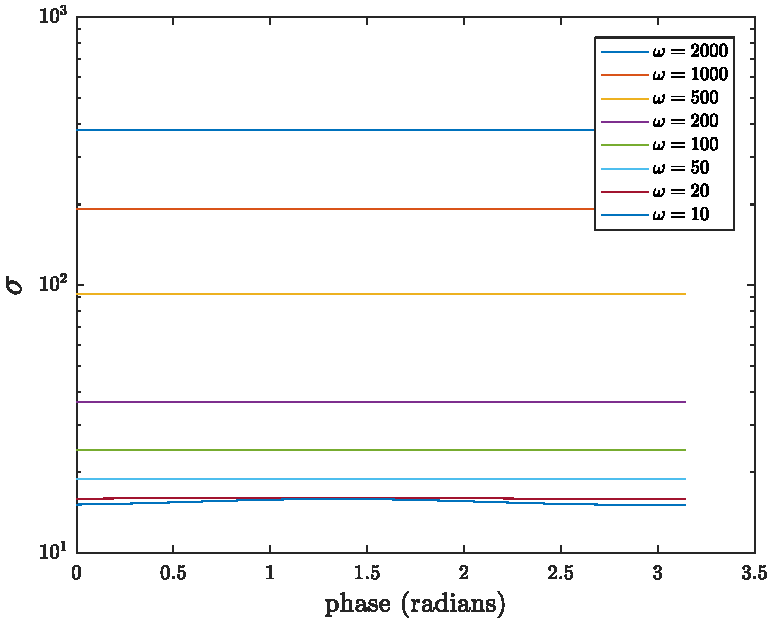
\includegraphics[width=0.5\textwidth]{phase_2D.pdf}
	\caption{Forecast error bars $\sigma^{T+E}$ versus the phase $\phi$. Apart from the smallest frequency $\omega=10$, the error bar remains almost constant. This implies that the sine ($\phi=0$) and cosine ($\phi=\pi/2$) feature models can be constrained independently.}
	\label{forecast_phase_dependence}
\end{figure}

\subsection{$l_\text{max}$ dependence}

Figure \ref{forecast lmax dependence} shows the graph of the forecast error bar $\sigma_{\sin}^{T+E}$ as we increase $l_\text{max}$. The forecasts were done within angular scale range $2\le l \le l_\text{max}$, the oscillation frequency $\omega$ set to 100, and assuming 1' beam and 1$\mu K\cdot$arcmin noise. The Planck noise curves were approximated by ones for 5' beam and 47 $\mu K\cdot$arcmin noise for this plot only since we extend $l_\text{max}$ to 4000 here. 

The Planck error bar essentially stalls out when $l_\text{max}$ reaches 2000. The forecast error bar, on the other hand, keeps decreasing until $l_\text{max}=4000$ thanks to the improved sensitivity in measuring small scales (and large $l$'s). Despite the information loss due to smaller sky coverage $f_\text{sky}$, the forecast error bar reduces to about 42\% of Planck by $l_\text{max}=4000$. This corresponds to a factor of 2.4 times improvement to measurement precision on $f_\text{NL}$.

\begin{figure}[ht]
	\centering
	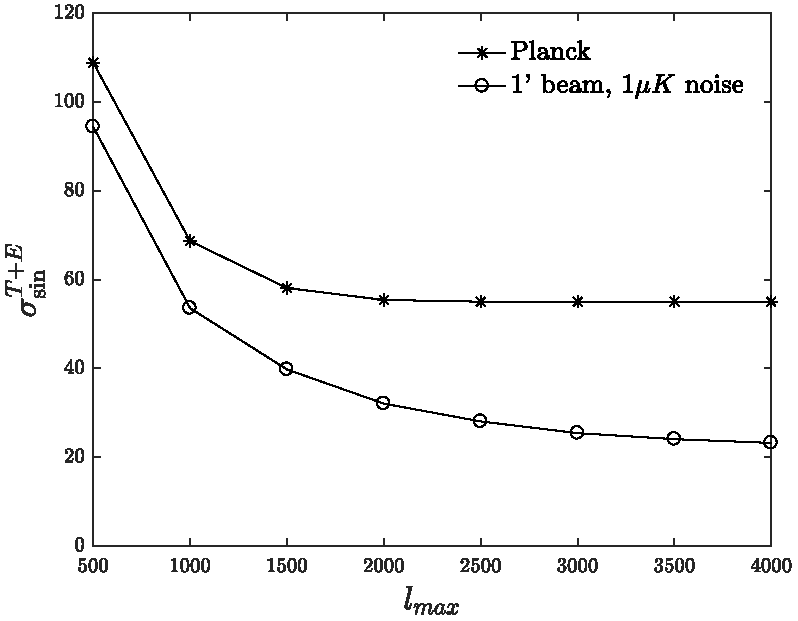
\includegraphics[width=0.5\textwidth]{lmax_dependence.pdf}
	\caption{Forecast error bars $\sigma_{\sin}^{T+E}$ when multipoles $2\le l \le l_\text{max}$ are included, in comparison with Planck. The oscillation frequency $\omega$ is set to 100 Mpc in all cases. Planck did not have access to the information from modes $l\ge 2000$, but CMB-S4 is expected to be able to explore modes up to $l=4000$.}
	\label{forecast lmax dependence}
\end{figure}

\subsection{Beam and noise dependence}

Now we explore the effects of different beam widths and noise levels on the forecast error bars. Figure \ref{forecast beam and noise dependence} shows forecast $\sigma_{\sin}^{T+E}$ for ranges of beam and noise levels. Their oscillation frequencies are also varied, but only two representatives $\omega=20$ and $2000$ are chosen here. Forecasts for the other values of $\omega$ also display similar dependences on beam widths and noise levels.

First of all, note that all estimated error bars in the plot are smaller than Planck, for which $\sigma_{\sin}^{T+E}=34$ when $\omega=20$ and $\sigma_{\sin}^{T+E}=610$ when $\omega=2000$. In fact, even the least sensitive CMB-S4 specification of 5' beam and 9$\mu K\cdot$arcmin noise is expected to put better bounds on feature models. Note that $l_\text{max}=4000$ for both $T$ and $E$ here.

Wider beams and noisier detectors provide less signal and thus larger error bars, as expected. In this range of beam width and noise levels, noise has a bigger effect on the forecast; experiments with 1' beam and 5$\mu K\cdot$arcmin noise yields larger error bars than the ones with 5' beam with 1$\mu K\cdot$arcmin noise. Between the most sensitive specification of 1' beam and 1$\mu K\cdot$arcmin and the least sensitive one with 5' beam and 9$\mu K\cdot$arcmin, $\sigma_{\sin}$ differs by a factor of 1.6.


\begin{figure}[ht]
	\centering
	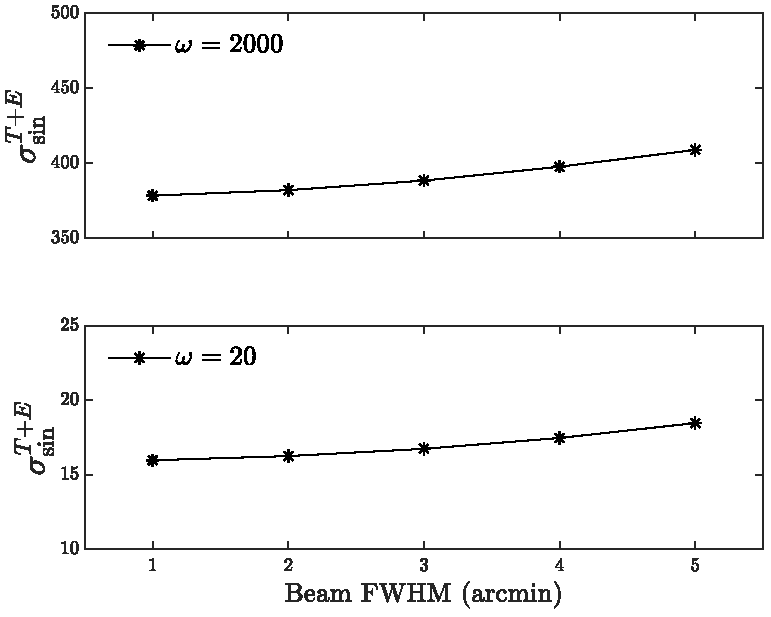
\includegraphics[width=0.45\textwidth]{beam_dependence.pdf}
	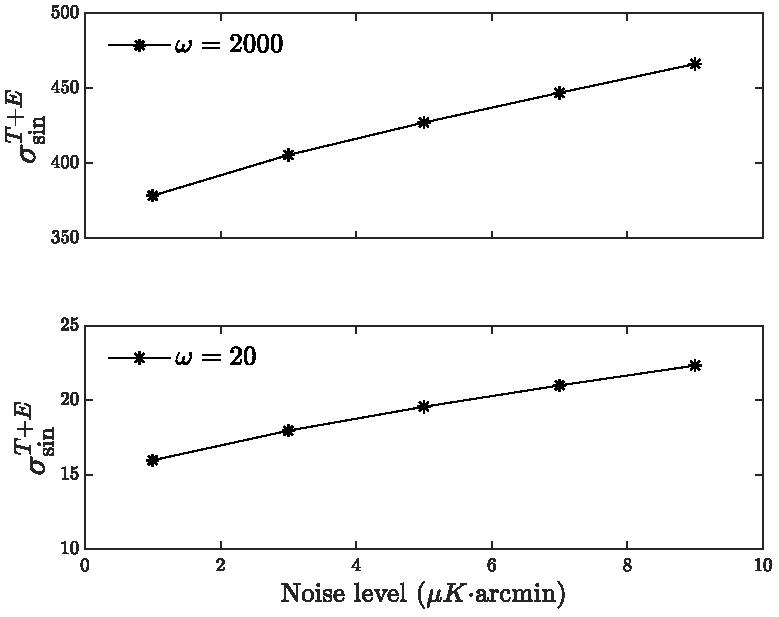
\includegraphics[width=0.45\textwidth]{noise_dependence.pdf}
	\caption{Beam (left) and noise (right) dependences of the forecast error $\sigma_{\sin}^{T+E}$ for $\omega=2000$ (top) and $\omega=20$ (bottom). The noise level was set as 1$\mu K \cdot$arcmin for the first plot, while the second plot had a fixed beam FWHM of 1'. We obtain less information from using wider beam and noisier sensors, as expected.}
	\label{forecast beam and noise dependence}
\end{figure}

\subsection{Oscillation frequency dependence}

We present the main results of the forecast. Figure \ref{forecast omega dependence pol} summarises the $\sigma_{\sin}$ forecasts for several different CMB-S4 preliminary specifications, including the Simons Observatory (SO) baseline and goal. Note that the $1/f$ noise effect is incorporated in SO forecasts but not in other ones. We also provide 1$\sigma$ errors for joint estimators, for which Planck signals from the fraction of the sky not covered by CMB-S4 are combined via a simple inverse variance method; $\sigma_\text{joint}^{-2} = \sigma_\text{CMB-S4}^{-2} +  \sigma_\text{Planck}^{-2}$. This is not statistically optimal but serves as a conservative estimate of the joint estimation power.

The most sensitive setup with 1' beam and 1$\mu K \cdot$arcmin noise would yield error bars that are 47-62\% of Planck. These correspond to a factor of 1.6-2.1 improvements. Here relatively smaller improvements are made for high oscillation frequencies. They correspond to smaller momentum scales $k_\ast = 2\pi/3\omega$, or larger angular scales, which benefit less from the increased sensitivity of CMB-S4. When the results are combined with Planck, the error bar reduces to 45-57\% of Planck, or a factor of 1.7-2.2 improvement.

Forecast error bars from the SO baseline specification and the more ambitious one (`goal') do not differ very much. Quoting in terms of the baseline values, $\sigma_{\sin}$ lies about 68-86\% of that of Planck or equivalently, 1.2-1.5 times smaller than Planck. Numbers change to 62-74\% when combined with Planck, so the overall improvement ratio is about 1.3-1.6.

\begin{figure}[ht]
	\centering
	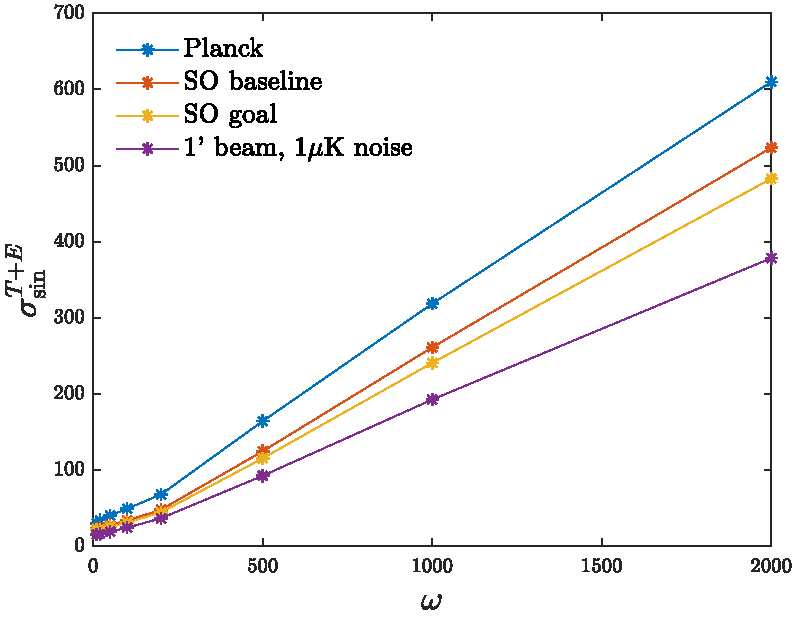
\includegraphics[width=0.45\textwidth]{omega_dependence_pol.pdf}
	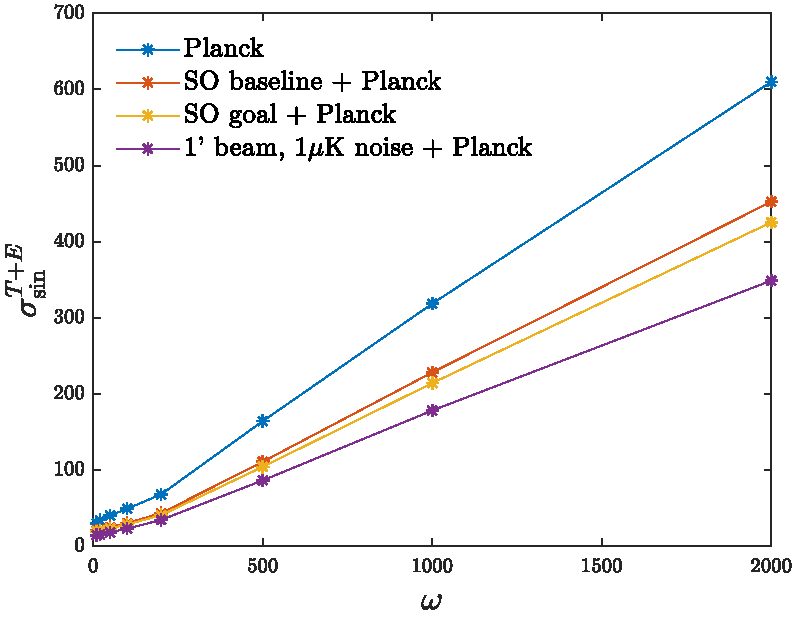
\includegraphics[width=0.45\textwidth]{omega_dependence_combined_pol.pdf}
	\caption{Frequency dependence of the forecast error in comparison to Planck (left). All CMB-S4 specifications would improve constraints on feature models. The most sensitive setup with 1' beam and 1$\mu K \cdot$arcmin noise is expected to yield error bars that are 1.6-2.1 times smaller than Planck. When the Planck results are combined with CMB-S4, we get even stronger constraints (right).}
	\label{forecast omega dependence pol}
\end{figure}

Figure \ref{forecast omega dependence T} shows the results when only the CMB temperature data are used in the forecast. CMB-S4 would in fact be worse than Planck in terms of constraining $f_\text{NL}^\text{feat}$ for this case. The loss in information due to less sky coverage overwhelms the increased sensitivity. We see again that the real strength of CMB-S4 lies in measuring CMB polarisation.

\begin{figure}[ht]
	\centering
	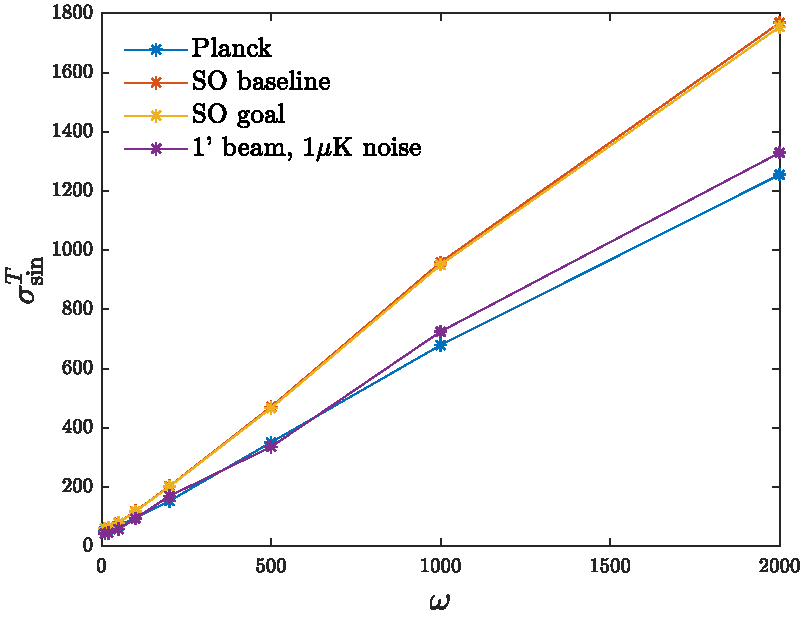
\includegraphics[width=0.45\textwidth]{omega_dependence_T.pdf}
	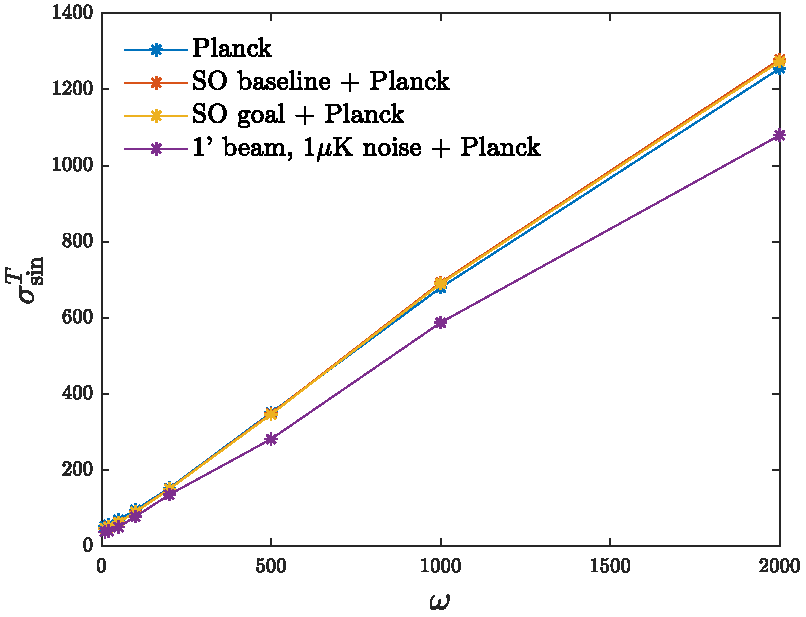
\includegraphics[width=0.45\textwidth]{omega_dependence_combined_T.pdf}
	\caption{Frequency dependence of the forecast error from temperature data only, in comparison to Planck (left). CMB-S4 would perform worse than Planck when only the temperature map is concerned. After the addition of Planck data the error bars improve only marginally (right). This shows that polarisation data is crucial for constraining feature models.}
	\label{forecast omega dependence T}
\end{figure}

Then how much information do we actually gain from adding E-mode polarisation? Figure \ref{forecast improvement ratio} shows the ratio of $\sigma_{\sin}$s between the temperature-only and polarisation-included analyses. The forecast error bars reduce up to 4.6 times smaller when polarisation information is added, which is much larger than the corresponding Planck value of 2.2. The ratio decreases overall when the joint statistics with Planck are considered. An intriguing feature of this plot is that the ratio is maximised around $\omega=200$ before it starts dropping again.

\begin{figure}[ht]
	\centering
	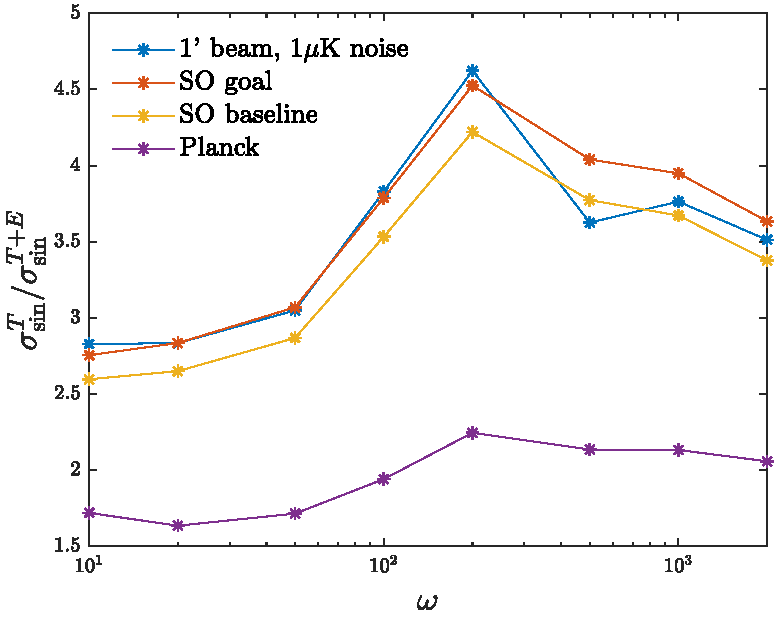
\includegraphics[width=0.45\textwidth]{improvement_ratio.pdf}
	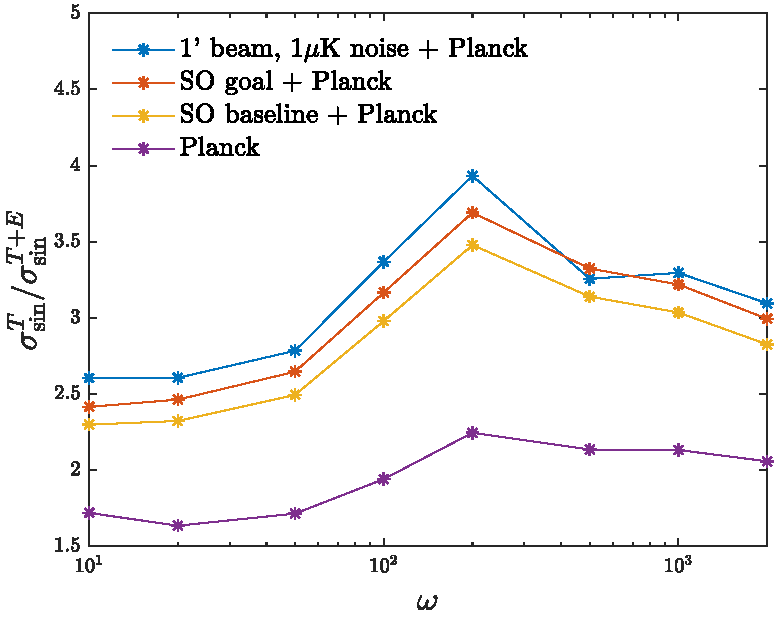
\includegraphics[width=0.45\textwidth]{improvement_ratio_combined.pdf}
	\caption{Improvements on the forecast error when including E-mode polarisation data. Constraints from CMB-S4 would improve significantly from addition of the polarisation data. The improvement is maximised around $\omega\approx200$ Mpc.}
	\label{forecast improvement ratio}
\end{figure}

In order to gain insight into this behaviour, we performed some simplified computations using the power spectrum. We imposed oscillations on the primordial power spectrum as $P_\textrm{feat}(k) = P(k)(1+\sin(2\omega k + \phi))$, which is just like our feature model bispectrum template but with $\omega(k_1+k_2+k_3)$ replaced by $\omega(k+k)$. $P_\textrm{feat}(k)$ is then projected to the late-time harmonic space using the transfer functions;
\begin{equation}
	C_{\text{feat},l}^{X_1 X_2} = \frac{2}{\pi} \int k^2 dk P_\textrm{feat}(k) \Delta_l^{X_1}(k) \Delta_l^{X_2}(k).
	\label{primordial power spectrum to cls}
\end{equation}
We observed that the fractional variation $(C_{\text{feat},l}-C_l)/C_l$ displays some oscillations in $l$, and the largest contribution comes from a term $\propto \sin(2\omega l/\Delta\tau)$ where $\Delta\tau$ represents the conformal distance to the last scattering surface. This fact can be explained by approximating the transfer function as $\Delta_l(k)\approx (1/3)j_l(k\Delta\tau)$ and noting that the spherical Bessel function has a sharp peak at $l$ for large $l$'s. The integral in (\ref{primordial power spectrum to cls}) therefore picks up a term proportional to $\sin(2\omega l/\Delta\tau)$.

The amplitude of these `maximal' oscillations in $(C_l'-C_l)/C_l$ were then computed using discrete Fourier transform for different values of oscillation scale $\omega$ and two different phases $\phi=0,\pi/2$ (i.e. sine and cosine). The results are shown in Figure \ref{insight feature plot}. Some extra wiggles to the graph come from the phase of oscillations imposed; we indeed see that graphs of sine and cosine oscillate between each other. Some peak features near $\omega\approx70$ and 140 arise from resonances with Baryonic Acoustic Oscillations.

We can think of the computed amplitude as a measure of information $C_l$'s contain about the primordial oscillations. First of all, note that the amplitude in all four plots generally decreases as $\omega$ grows. Previously in Figure \ref{forecast omega dependence pol} we saw that the amount of information obtained from the CMB is smaller for larger $\omega$'s, consistent with what can be said from the amplitude analysis. Moreover, the amplitudes for the EE mode are generally larger than the TT mode ones, and their difference is the largest in the $\omega$ range of 70 to 300. This could serve as a heuristic explanation for the improvement in forecast error bars from including polarisation data being maximised around $\omega=200$, as depicted in Figure \ref{forecast improvement ratio}.

\begin{figure}[ht]
	\centering
	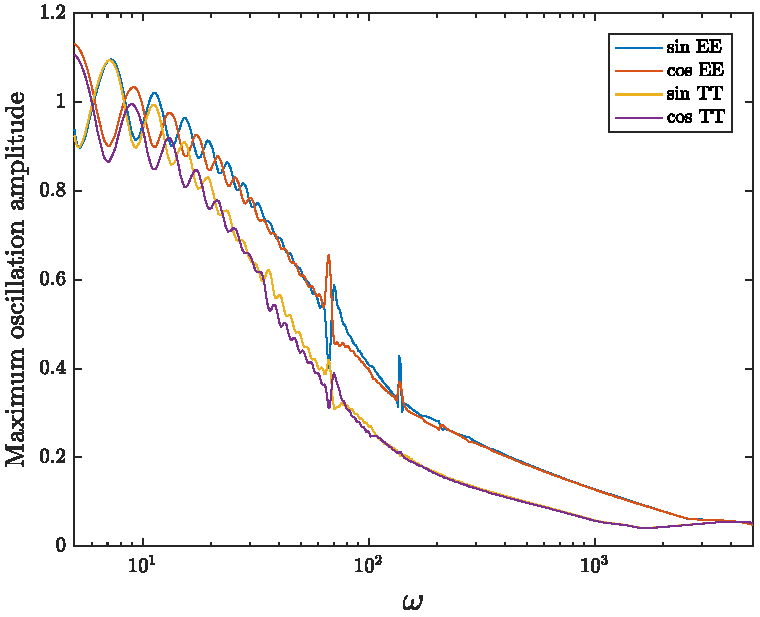
\includegraphics[width=0.7\textwidth]{feature_plot.pdf}
	\caption{The maximum amplitude of oscillations detected in fractional variations of the projected power spectrum $C_l^{TT}$ and $C_l^{EE}$, when extra oscillations $\sin(2\omega k)$ and $\cos(2\omega k)$ were imposed on the primordial power spectrum. Heuristically this shows that E-mode polarisation is more sensitive to the primordial oscillations, especially in the $\omega$ range of 70 to 300. Some peaks near $\omega=70$ and $140$ arise from resonances with Baryonic Acoustic Oscillations. }
	\label{insight feature plot}
\end{figure}


\subsection{Comparison to scale-invariant models}

Our pipeline for forecasting $f_\text{NL}^\text{feat}$ also yields forecasts for $f_\text{NL}$ of the constant model, which is scale-invariant and have a trivial shape; $B(k_1,k_2,k_3) \propto (k_1 k_2 k_3)^{-2}$.
Forecasts on $f_\text{NL}^\text{const}$ follow from our pipeline by simply setting the oscillation frequency $\omega = 0$ and phase $\phi = \pi/2$. Table \ref{forecast constant model} summarises the forecast results for several different CMB-S4 specifications mentioned before, using both T and E data and in combination with Planck data from the regions of the sky not covered by CMB-S4. For the 1' beam and 1$\mu K \cdot$arcmin noise setup, the error bar is expected to be reduced by a factor of 2.3 compared to Planck.

\begin{table}[ht]
	\caption{Forecasts on the estimation errors of $f_\text{NL}$ for the constant model}
	\centering
	\label{forecast constant model}
	\renewcommand{\arraystretch}{1.4}
	\begin{tabular}{ccccc}
		\toprule
		& Planck  & SO baseline + Planck & SO goal + Planck & 1' beam, 1$\mu K$ noise + Planck \\
		\midrule
		$\sigma(f_\text{NL}^\text{const})$ & 23.4 & 14.9 & 14.0 & 10.4 \\
		\bottomrule
	\end{tabular}
\end{table}

The latest Planck constraints on $f_\text{NL}$ of some popular bispectrum templates are given by $f_\text{NL}^\text{local} = 2.5 \pm 5.7$, $f_\text{NL}^\text{equil} = -16 \pm 70$, and $f_\text{NL}^\text{ortho} = -34 \pm 33$ \cite{PlanckCollaboration2015}. CMB-S4 is expected to yield better estimates on these as well. Table \ref{forecast various models} summarises the forecast improvement ratio given in \cite{Abazajian2016} together with the constant and feature model ratios computed in this work.

\begin{table}[ht]
	\caption{Expected improvement ratios of the $f_\text{NL}$ estimation errors for the CMB-S4 1'beam, 1$\mu K$arcmin setup, for various bispectrum templates. The local, equilateral and orthogonal results are quoted from \cite{Abazajian2016}.}
	\centering	
	\label{forecast various models}
	\renewcommand{\arraystretch}{1.4}
	\begin{tabular}{cccccc}
		\toprule
		& Local & Equilateral & Orthogonal & Constant & Feature ($\omega=200$) \\ \midrule
		$\sigma^\text{Planck}/\sigma^\text{CMB-S4}$ & 2.5   & 2.1         & 2.4        & 2.3      & 2.0                \\
		\bottomrule
	\end{tabular}
	
\end{table}

Surprisingly, the estimation error for feature models does not improve as much as other templates. Feature models benefit much more from the inclusion of polarisation data than any other scale-independent shapes; for example, $\sigma^{T}/\sigma^{T+E} = 4.6$ for the feature models with $\omega=200$ in CMB-S4 while the value equals 2.8 for the constant models. Because CMB-S4 would have a significantly enhanced polarisation measurement sensitivity, we originally expected the feature models to be constrained significantly better than Planck.

In order to investigate this lack of improvement, we performed a breakdown analysis on the improvements gained from CMB-S4 temperature and polarisation; we computed $\sigma(f_\text{NL})$ for the constant and feature models using each of the four combinations of Planck / CMB-S4 noise curves for temperature / polarisation (e.g. Planck T + CMB-S4 E). The results are summarised in Table \ref{forecast mixed}.

\begin{table}[ht]
	\caption{Expected improvements on the estimation errors of $f_\text{NL}$ for each combination of Planck / CMB-S4 temperature (T) and polarisation (E) data. Here the CMB-S4 assumes 1' beam and 1$\mu K$arcmin noise. The feature model has oscillation frequency $\omega=200$ and phase $\phi=0$. The sky fraction $f_\text{sky}=0.4$ for all cases except for Planck T + Planck E, for which $f_\text{sky}=0.76$.}
	\centering
	\label{forecast mixed}
	\renewcommand{\arraystretch}{1.5}
	\begin{tabular}{c c c c c c c c}
		\toprule
		\multicolumn{2}{c}{$\sigma(f_\text{NL}^\text{const})$}  &  \multicolumn{2}{c}{E}  & \multicolumn{2}{c}{$\sigma(f_\text{NL}^\text{feat})$}  &  \multicolumn{2}{c}{E}  \\
		\cmidrule(lr){3-4} \cmidrule(lr){7-8} 
		\multicolumn{2}{c}{improvements}  & Planck & CMB-S4 & \multicolumn{2}{c}{improvements}  & Planck & CMB-S4 \\
		\cmidrule(lr){1-4} \cmidrule(lr){5-8}
		\multirow{2}{*}{T} & Planck & 1.0 & 1.6 & \multirow{2}{*}{T} & Planck & 1.0 & 1.7 \\
		& CMB-S4 & 1.1 & 2.2 & & CMB-S4 & 0.9 & 2.0 \\
		\bottomrule
	\end{tabular}
\end{table}



We see that the constraints on feature models improve by a factor of 1.7 when swapping Planck polarisation noises with the CMB-S4 ones. This factor is indeed larger than 1.6 of the constant model. The difference is however not significant. It seems that the amount of feature signals in polarisation data left unexplored by Planck is not tremendously large compared to the constant model. The feature model improves less than the constant model when the temperature measurements are enhanced. In fact, for feature models, the signal loss from smaller sky fraction $f_\text{sky}$ eclipses the signal gain from more sensitive temperature measurements. This lack of improvements from temperature causes the full CMB-S4 constraints on the feature model not to improve as much as the constant model overall.

\newpage
\section*{Summary} 

Upcoming CMB Stage-4 experiments will provide an opportunity to measure the CMB temperature anisotropies and polarisation with ever greater precision. The CMB bispectrum estimators for constraining primordial non-Gaussianity would greatly benefit from the improvement in measurement sensitivity. In this research, we made forecasts on the $f_\text{NL}$ for feature models, which have not been done so far despite the growing interest in inflation models with oscillations in the primordial spectrum. For efficient forecasts we simplified the bispectrum estimator for $f_\text{NL}$ by orthonormalising the covariance matrix, further optimising the computation. When the most sensitive CMB Stage-4 experiment specification of 1' beam and 1$\mu K$arcmin noise is concerned, we expect a factor of 1.7-2.2 times more stringent constraints compared to Planck. Under the realistic Simons Observatory conditions, the improvement would be about 1.3-1.6 to Planck.

Although this is not a massive boost in the estimation power, we can hope to verify the current 4$\sigma$-level signals found in the Planck 2015 analysis. It is also worth noting that CMB-S4 would allow us to explore the modes with $l>2000$ and localised oscillations on these scales are currently unconstrained. Moreover, though we have only considered linearly-spaced oscillations in this work, we expect even better improvements on the models inducing logarithmically-spaced oscillations where small scale modes with higher $l$ would greatly enhance the constraining power. Lastly, we can expect to cross-validate using these new statistically independent modes to test current constraints further.

We also extensively studied how the forecasts depend on various parameters. Frequency dependences of the ratio between the T and T+E forecasts were particularly illuminating; the improvement from adding polarisation information is maximised around $\omega = 200$. Some simplified calculations were presented to heuristically address this fact. Even though the estimation power on feature models massively benefits from the polarisation data, the expected improvements compared to Planck are quite underwhelming overall. A breakdown analysis of the temperature and polarisation contribution revealed that the feature models would indeed improve more than other scale-independent models if only the polarisation (and not temperature) measurement sensitivity were enhanced to the CMB-S4 standards. However, boosts in the temperature measurements affect scale-independent models more so that they gain more information overall.

The KSW estimator utilises separable bispectrum templates to constrain $f_\text{NL}$ exactly even for highly oscillatory models but is inherently restrictive in the range of shapes it can handle. On the other hand, the Modal estimator uses separable basis functions to expand the given bispectrum shape and thus is able to cover a broad range of non-separable shapes. Due to limitations such as the basis size, however, its accuracy drops for oscillatory models with high frequency. Hence, currently, there is a blind spot in the bispectrum analysis for general (non-separable) \textit{and} highly oscillatory models barred  by numerical challenges. We address this in our original research on the high-resolution CMB bispectrum estimator in Chapter \ref{chapter:high_resolution_cmb_bispectrum_estimator}.

\clearpage{}
\clearpage{}\chapter{High-Resolution CMB Bispectrum Estimator} \label{chapter:high_resolution_cmb_bispectrum_estimator}

\ifpdf
    \graphicspath{{Chapter5/Figs/Raster/}{Chapter5/Figs/PDF/}{Chapter5/Figs/}}
\else
    \graphicspath{{Chapter5/Figs/Vector/}{Chapter5/Figs/}}
\fi

Despite their major role in constraining a wide range of inflation models, there are only a few implementations of the CMB bispectrum estimator due to computational challenges. The Planck collaboration mainly utilised three independent approaches for their bispectrum analysis \cite{PlanckCollaboration2013,PlanckCollaboration2015,PlanckCollaboration2018}: KSW \cite{Komatsu2005}, Modal \cite{Fergusson2012}, and Binned \cite{Bucher2010}. Standard bispectrum templates for Local, Equilateral and Orthogonal shapes have been constrained using all three methods independently, whilst other more specific ones were covered by only a subset of them.

Some of the most challenging models to handle are those with oscillatory behaviour. Numerous theoretically well-motivated models (\cite{Chen2010foldedResonant,Meerburg2009signatures,Meerburg2010nbd,Meerburg2011cutoff,Hazra2014} and many more, see e.g., \cite{Chen2010review,Chen2016} for reviews) fall into this category. Feature models, as discussed in the previous chapter, often predict linearly spaced oscillations in the bispectrum. Resonance models such as axion monodromy inflation \cite{Silverstein2008monodromy,Flauger2010monodromy} produce log-spaced oscillations modulated with various envelopes. Constraining such models is difficult since oscillations in the bispectra degrade the numerical stability of the integrals involved.

Several simple models with oscillations have been studied in the latest Planck analysis using Modal and a few specific KSW-type estimators introduced in \cite{Munchmeyer2014}. Modal estimator covers a wide range of oscillatory models, both with and without envelopes, thanks to the versatility of its mode expansion. It is however difficult to constrain models with high-frequency oscillations using generic mode functions. Modal code allows for choosing a more tailored set of modes for this purpose, but the fact that there are \textit{two} independent sets of mode functions - primordial and late-time - complicates targeted analyses. For each specific selection of mode functions in the primordial `$k$' domain, a suitable choice of basis has to be made in the late-time `$l$' space. Rapidly oscillating signals may also get lost during the projection from one to the other and cause some numerical issues.

On the other hand, adapted KSW-type estimators \cite{Munchmeyer2014,Munchmeyer2015resonance,Meerburg2016jointResonance} may probe models with much faster oscillations in their bispectra. They exploit the separability of specific oscillatory templates and/or Fourier-type bases to obtain accurate constraints on a model-by-model basis. However, these methods are not easily applicable for models with more complicated bispectra, especially the ones that do not depend solely on $K=k_1+k_2+k_3$. The formalism is also restricted to certain types of bispectra and requires a separate implementation for each case. This was one of the main motivations behind the research project; can we have a bispectrum estimator which has the efficiency and versatility of Modal, whilst also benefiting from the precision of the KSW formalism for a more specialised analysis?

We developed a novel CMB bispectrum estimation pipeline \textsc{CMB-BEst}. \footnote{Short for \underline{CMB} \underline{B}ispectrum \underline{Est}imator. The goal of \textsc{CMB-BEst} is to be the best bispectrum estimator with wide applications and great precision.} \textsc{CMB-BEst} has two main strengths over former methods. First of all, it is implemented for completely general basis sets, which allows broad analyses of inflationary models. In fact, the conventional KSW estimator is equivalent to a specific choice of basis in \textsc{CMB-BEst}. \textsc{CMB-BEst} can cover any model KSW estimator can, and furthermore, it can simultaneously constrain general bispectrum shapes through primordial mode expansion, just like Modal.

Secondly, \textsc{CMB-BEst} is designed to be able to handle complex and highly oscillatory signals. It does not require a separate set of basis functions for late-time $l$ space, contrary to Modal. More diverse and specialised choices of basis can therefore be made. The code will be used on numerous inflation models with complex oscillations which are yet to be investigated due to lack of resolution from previous methods. Potential choices of the targeted basis for this purpose will be discussed in Section \ref{section:basis_functions}.

Every good thing comes at a price. For \textsc{CMB-BEst}, the price is computational cost. Combining the best of Modal and KSW estimators, \textsc{CMB-BEst}'s formalism is more numerically demanding than both of them. Na\"ively speaking, running \textsc{CMB-BEst} for one set of basis functions is equivalent to computing thousands of KSW estimators put together. It is prohibitively expensive unless properly and thoroughly optimised.

We invested a considerable amount of time and effort in optimising the code. Separable mode expansions and subsequent algorithm design were studied in detail for a maximal reduction in computational complexity. We also made full use of parallelisation techniques to exploit modern computing architecture. Improving data locality for efficient memory access yielded an order of magnitude speed-up. We illustrate our optimisation procedure in Section \ref{section:implementation}.

The code was then tested thoroughly both internally and against Planck analysis. We used CMB maps and simulations from the Planck satellite experiment and checked that \textsc{CMB-BEst} agrees with previous routines map-by-map for various bispectrum templates. Different choices of basis functions within \textsc{CMB-BEst} also yielded consistent results. We dedicate Section \ref{section:validation} to presenting the outcome of these consistency checks.

Lastly, we present some applications of the code which serve as a proof of concept. In particular, we connect \textsc{CMB-BEst} to \textsc{Primodal}, an efficient numerical code for computing bispectra of primordial perturbations from a given single field model \cite{Clarke2021}. \textsc{Primodal} uses separable modes for its computation, which enables template-free, direct model-to-constraint analysis when combined with \textsc{CMB-BEst} appropriately. Section \ref{section:proof_of_concept} highlights some results from the combined pipeline. We also identify areas where improvements could be made and discuss directions for future research.

Upcoming surveys will provide major improvements to constraints on primordial non-Gaussianity. Inflationary models with oscillations would also greatly benefit from the enhanced sensitivity, as we discussed in the previous chapter. It is therefore crucial to have a robust and flexible bispectrum estimation routine ready for future surveys, especially one which can handle high-frequency oscillations. Having another code independent from the existing ones would also be greatly beneficial for cross-validation. We expect \textsc{CMB-BEst} to fill this role in the near future.


\section{Formalism}

\subsection{\textsc{CMB-BEst} formalism}
Recall that the optimal CMB bispectrum estimator for a given template can be written as
\begin{align}
	\hat{f}_\text{NL} = \frac{1}{N} \sum_{l_j,m_j} \frac{\mathcal{G}^{l_1 l_2 l_3}_{m_1 m_2 m_3} b_{l_1 l_2 l_3}}{C_{l_1} C_{l_2} C_{l_3}} \left[ a_{l_1 m_1} a_{l_2 m_2} a_{l_3 m_3} - \left( \left< a^G_{l_1 m_1} a^G_{l_2 m_2} \right> a_{l_3 m_3} + \text{2\ cyc.} \right)  \right].		\label{eqn:bispectrum_estimator_standard}
\end{align}
Here we omit superscripts $X$ for temperature and polarisation for notational convenience. Even though the formalism in this section will be presented for CMB temperature data only, the method is general and can easily be extended to include polarisation. For estimation of the full covariance matrix $C_{lm,l'm'}$ needed for the linear term, we use an ensemble average from Gaussian simulations, as denoted by superscripts $G$ and the bracket $\left<\cdot\right>$.

The normalisation factor is given by
\begin{align}
	N = \sum_{l_j} \frac{h_{l_1 l_2 l_3}^2 b_{l_1 l_2 l_3}^2}{C_{l_1} C_{l_2} C_{l_3}}.
\end{align}

The core part of our estimation routine is the separable mode expansion of the shape function;
\begin{align}
	S(k_1, k_2, k_3) := (k_1 k_2 k_3)^2 B(k_1, k_2, k_3) = \sum_{p_j} \alpha_{p_1 p_2 p_3} q_{p_1}(k_1) q_{p_2}(k_2) q_{p_3}(k_3).
\end{align}
Choices for the basis functions $q_p(k)$ are detailed in the next section. Due to the separability, the reduced bispectrum reduces to a compact form of
\begin{align}
	b_{l_1 l_2 l_3} = \sum_{p_j} \alpha_{p_1 p_2 p_3} \int dr \tilde{q}_{p_1}(l_1,r) \tilde{q}_{p_2}(l_2,r) \tilde{q}_{p_3}(l_3,r),
\end{align}
where the \textit{projected} mode functions are defined as
\begin{align}
	\tilde{q}_{p}(l,r) := \frac{2r^\frac{2}{3}}{\pi} \int dk q_p(k) \Delta_l(k) j_l (kr).
\end{align}
Radiative transfer functions $\Delta_l(k)$ and spherical Bessel functions $j_l(kr)$ are denoted the same way as in the previous chapter.

Every term appearing in (\ref{eqn:bispectrum_estimator_standard}) except the Gaunt integral is now separable. Using the definition $\mathcal{G}^{l_1 l_2 l_3}_{m_1 m_2 m_3} = \int d^2 \vv{n} Y_{l_1 m_1}(\vv{n}) Y_{l_2 m_2}(\vv{n}) Y_{l_3 m_3}(\vv{n})$, we can render it separable at the cost of introducing an extra integral.

We define the filtered maps as
\begin{align}
	M^{(i)}_p (\vv{n}, r) := \sum_{l,m} \frac{\tilde{q}_p (l,r)}{C_l} a^{(i)}_{lm} Y_{lm} (\vv{n}), \label{def:filtered_maps}
\end{align}
where $a^{(i)}_{lm}$'s are represent the spherical harmonic transform of the $i$th CMB map. For later convenience, we use a convention where $i=0$ corresponds to the observed CMB map. Maps number $1$-$N_\text{sims}$ are Gaussian simulations. Note that without the factors involving $\tilde{q}$ and $C_l$'s, $M$ is simply equal to the original map in real space. Each mode extracts different anisotropy scales present on the map.

The bispectrum estimator (\ref{eqn:bispectrum_estimator_standard}) reduces to
\begin{align}
	\hat{f}_\text{NL}^{(i)} = \frac{1}{N} \sum_{p_j} \alpha_{p_1 p_2 p_3} (\beta^{\textrm{cub},(i)}_{p_1 p_2 p_3} - 3 \beta^{\textrm{lin},(i)}_{p_1 p_2 p_3}), \label{eqn:fNL_from_betas}
\end{align}
where most of the computation required is now contained in the `$\beta$'s, given by
\begin{align}
	\beta^{\textrm{cub},(i)}_{p_1 p_2 p_3} &:= \int dr \int d^2\vv{n} \; M^{(i)}_{p_1} (\vv{n},r) M^{(i)}_{p_2} (\vv{n},r) M^{(i)}_{p_3} (\vv{n},r),	\label{def:beta_cubic} \\
	\beta^{\textrm{lin},(i)}_{p_1 p_2 p_3} &:= \frac{1}{N_\text{sims}} \sum_{j \neq i} \int dr \int d^2\vv{n} \; M^{(j)}_{p_1} (\vv{n},r) M^{(j)}_{p_2} (\vv{n},r) M^{(i)}_{p_3} (\vv{n},r). \label{def:beta_linear}
\end{align}
Here we evaluate $f_\text{NL}$ estimates for each of the Gaussian simulations $i=1,\cdots,N_\text{sims}$. Naturally, they are normally distributed with a mean of zero. Under the null hypothesis that the initial fluctuations are purely Gaussian, the value of $f_\text{NL}$ estimated from the observed CMB map is also drawn from the same normal distribution. Any statistically significant deviations from zero would therefore allow us to reject the null hypothesis.

It is important to note that the $\beta$ matrices depend only on the choice of mode functions and input map data, and are independent of the theoretical bispectrum considered. Once $\beta^\text{cub}$ and $\beta^\text{lin}$ are computed and stored, we may constrain any model of interest by decomposing the template to get $\alpha$. The $f_\text{NL}$ estimate is then  a simple dot product: $\vv{\alpha} \cdot \vv{\beta} / N$.

The normalisation can also be obtained in a similar fashion;
\begin{align}
	N = \sum_{p_j, p'_j} \alpha_{p_1 p_2 p_3} \Gamma_{p_1 p_2 p_3, p'_1 p'_2 p'_3} \alpha_{p'_1 p'_2 p'_3}, \label{eqn:normlisation_from_gamma}
\end{align}
or equivalently, $N = \vv{\alpha}^T \Gamma \vv{\alpha}$. We exploit separability once again to compute the $\Gamma$ matrix;
\begin{align}
	\Gamma_{p_1 p_2 p_3, p'_1 p'_2 p'_3} &:= \int dr \int d\mu \mathcal{P}_{p_1 p'_1}(\mu, r, r') \mathcal{P}_{p_3 p'_3}(\mu, r, r') \mathcal{P}_{p_3 p'_3}(\mu, r, r'), 	\label{def:gamma} 	\\
	\mathcal{P}_{p p'}(\mu, r, r') &:= \sum_l \frac{2l+1}{(8\pi)^{1/3} C_l} \tilde{q}_{p'}(l,r) \tilde{q}_p(l,r') P_l(\mu),
\end{align}
where $P_l(\mu)$'s are the Legendre polynomials.

In summary, \textsc{CMB-BEst} computes the main quantities: $\beta^\text{cub}$, $\beta^\text{lin}$, and $\Gamma$. The most computationally expensive part is the linear term $\beta^\text{lin}$ by a couple of orders of magnitude in most cases. Considerable effort has been made to optimise the corresponding part of the code, which will be detailed in the following sections.

\subsection{Basis functions} \label{section:basis_functions}

One of the greatest strengths of \textsc{CMB-BEst} lies in its flexibility with the choice of mode functions. We decompose a given shape as a linear combination mode function in three-dimensional space. Hence, we shall refer to them as `basis' functions. Adopting a specialised basis set provides optimised results to specific models of interest, whilst a more general construction of basis allows us to simultaneously constrain a wide range of models.

The main difference between \textsc{CMB-BEst} and the conventional Modal estimator \cite{Fergusson2010general} is that \textsc{CMB-BEst} has a single set of mode functions while Modal requires two; one in each of the primordial and late-time space (see section \ref{section:CMB_bispectrum_estimators}). While the Modal approach can accurately express a wide range of bispectra \cite{Fergusson2012,Fergusson2014,PlanckCollaboration2013}, the two-step modal expansion becomes less accurate for highly oscillatory shapes since the oscillations often get lost during the projection to late-time space \cite{Fergusson2015a,PlanckCollaboration2018}. \textsc{CMB-BEst} avoids these issues in the second mode expansion by evaluating an exact analytical form analogous to the KSW estimator \cite{Komatsu2005}. The results obtained from \textsc{CMB-BEst} is therefore as accurate as the primordial basis expansion.

We observe that the KSW estimator \cite{Komatsu2005} is derived from a simple monomial basis in our notation;
\begin{align}
	q_p(k) = k^{p-1}, \;\;\; p = 0, 1, 2, 3.
\end{align}
All three standard templates - local, equilateral, and orthogonal - can be expressed as a sum of separable terms in the form $q_{p_1}(k_1) q_{p_2}(k_2) q_{p_3}(k_3)$. The shape function of the local template, for example, is given by
\begin{align}
	S^\textrm{local}(k_1 k_2 k_3) :=& 2A^2 \left[ \frac{k_1^2}{k_2 k_3} + \frac{k_2^2}{k_3 k_1} + \frac{k_3^2}{k_1 k_2}  \right] \\
	=& 2A^2 \left[q_3(k_1)q_0(k_2)q_0(k_3) + q_0(k_1)q_3(k_2)q_0(k_3) + q_0(k_1)q_0(k_2)q_3(k_3) \right],
\end{align}
where $A$ is the primordial power spectrum amplitude. Decomposition coefficients $\alpha_{p_1 p_2 p_3}$ have three non-zero components: $\alpha_{300} = \alpha_{030} = \alpha_{003} = 2A^2$. Coefficients for the equilateral and orthogonal templates can similarly be found.

We set the scalar spectral index as $n_\text{s} = 1$ above for simplicity. For a non-unit $n_\text{s}$, we modify the basis as follows;
\begin{align}
	q_p(k) = k^2 \left[ k_* \left( \frac{k}{k_*} \right)^{(4-n_\text{s})/3} \right]^{p-3}, \;\; p=0,1,2,3. \label{eqn:KSW_basis}
\end{align}
The pivot scale $k_*$ is defined such that the power spectrum evaluates to $A$ at $k=k_*$. Including $k_*$ here ensures that the $q_p(k)$'s have the right units. Note that the prefactor $k^2$ comes from the definition of the shape function and is therefore unaffected by $n_\text{s}$. We will refer to this choice of mode functions to be the `KSW' basis.

For studying models with linearly spaced, high-frequency oscillation, a Fourier-like basis
\begin{align}
	q_0(k) = \sin (\omega k), \; q_1(k) = \cos (\omega k), \label{eqn:Fourier_basis}
\end{align}
for a fixed $\omega$ is an appropriate choice. This is in fact equivalent to the method we used to study feature models in Chapter \ref{chapter:CMB_state-4_forecast}. The small size of the basis lets us efficiently constrain theoretical models with given characteristic scale $\omega$. By scanning over a range of $\omega$, or including modes with different values of $\omega$ in the basis, we may also perform a more comprehensive analysis of oscillatory features.

Lastly, for investigating a wide variety of models simultaneously, we construct large basis sets suitable for decomposing general shape functions. One such example is the following basis which consists of Legendre polynomials;
\begin{align}
	q_p(k) = P_p(\bar{k}), \;\;\text{where}\;\; \bar{k} = \frac{2k-k_\text{min}-k_\text{max}}{k_\text{max}-k_\text{min}}.  \label{eqn:Legendre_basis_no_inv_k}
\end{align}
Here we linearly map the range from $k \in [k_\text{min},k_\text{max}]$ to $\bar{k} \in [-1,1]$, which is the interval where Legendre polynomials are defined. The number of modes are not bounded; the larger the basis, the more complete coverage of theory $k$ space we get.

The Legendre basis functions are inherently orthogonal, so that $\int_{-1}^{1} d\bar{k} P_{l}(\bar{k}) P_{l'}(\bar{k}) = 0$ whenever $l \neq l'$. Orthogonality is essential for this class of basis sets since it allows us to greatly simplify the way of decomposing theoretical templates. We elaborate on the decomposition method in Section \ref{section:primordial_basis_expansion}. 

The Legendre basis also enables direct connection to \textsc{Primodal}, a fast numerical code for computing primordial bispectra from general single-field inflation models \cite{Clarke2021}. \textsc{Primodal} utilises the inherent separability present in the \textit{in-in} formalism to efficiently compute the bispectrum using a separable basis. Using the Legendre polynomials for the basis is optimal for this step, but the methodology is not restricted to any particular choice of basis. The code then outputs the expansion coefficients of the primordial bispectrum with respect to the Legendre polynomials. Hence, the result can be plugged in directly to \textsc{CMB-BEst}, creating one fluid pipeline from the model Lagrangian to $f_\text{NL}$ estimation.

As noted in \cite{Clarke2021}, we may augment the base set of Legendre polynomials with one or more extra functions for a better description of some bispectrum templates. One solid choice is to add a mode $q(k) = k^{n_\text{s} -2}$, orthogonalised with respect to the rest of the basis. This significantly boosts the performance of decomposing local-type bispectra.

Ideally, we would like the $k$ range used in the definition (\ref{eqn:Legendre_basis_no_inv_k}) to be as wide as possible so that more information from different scales is incorporated in the estimation process. A wider $k$ range, however, also results in lower resolving power because the interval can fit more oscillations of a given frequency. Polynomials of higher degrees are necessary to handle the same bispectra. We found that $k_\text{max}/k_\text{min} = 1000$ is an overall sweet spot for analysing Planck data.

Throughout the rest of this thesis, we refer to a basis with the $k^{n_\text{s} - 2}$ mode and the first 29 Legendre polynomials, totalling 30 modes, defined in the $k$ range with $(k_\text{min}, k_\text{max}) = (2.09 \times 10^{-4}, 2.09 \times 10^{-1})$, as the `Legendre' basis. Any deviation from this set of parameters will be stated explicitly. Note that this is for our convenience during testing only; the code may take any choice of basis.


\subsection{Primordial basis expansion} \label{section:primordial_basis_expansion}

Our formalism assumes that the bispectrum shape of interest can be accurately represented as a linear combination of a chosen basis set; 
\begin{align}
	S(k_1,k_2,k_3) = \sum_{p_j} \alpha_{p_1,p_2,p_3} \; Q_{p_1 p_2 p_3}(k_1, k_2, k_3),
\end{align}
where the three-dimensional mode functions are defined as
\begin{align}
	Q_{p_1 p_2 p_3} (k_1, k_2, k_3) := q_{p_1}(k_1) \; q_{p_2}(k_2) \; q_{p_3}(k_3).
\end{align}
For some models, the coefficients $\alpha_{p_1 p_2 p_3}$ are obtained analytically. The local shape function with respect to the KSW basis is a simple example; $\alpha_{300}=\alpha_{030}=\alpha_{003}=2A^2$ and zero otherwise. For other models, the shape function needs to be expanded with respect to the chosen basis. 

Shape functions are defined on the same domain as bispectra: $(k_1,k_2,k_3) \in \mathbb{R}^3$ where $k_1$, $k_2$, and $k_3$ form a triangle. We cannot observe scales smaller than a certain size in practice, which places an upper bound on $k$: $k < k_\text{max}$. The resulting domain in three dimensions is shown in Figure \ref{fig:tetrapyd}.

\begin{figure}[htbp!] 
	\centering    
	\hspace{10pt}
	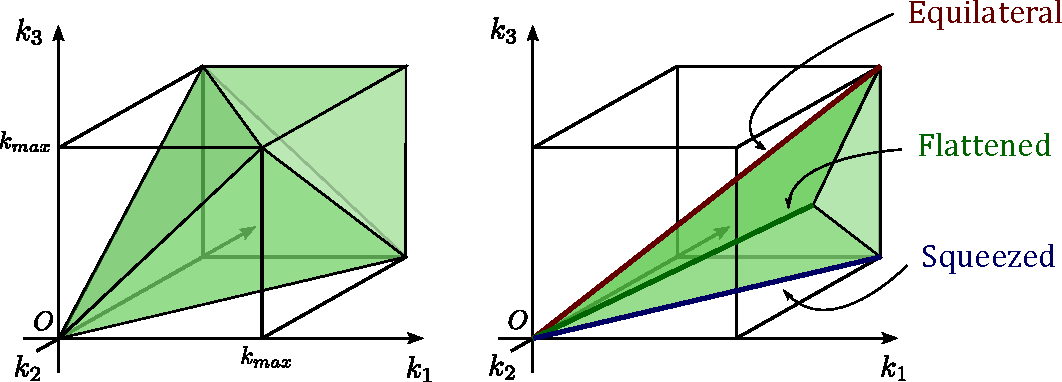
\includegraphics[width=1.0\textwidth]{tetrapyd.pdf}
	\caption{Tetrapyd domain in which the shape functions are defined. Left: the full region specified by triangle inequalities and an upper bound $k_\text{max}$. Right: one-sixth slice of the tetrapyd from which shape functions are uniquely determined by symmetry in the $k$'s. Edges representing the equilateral, flattened and squeezed configurations are annotated.}
	\label{fig:tetrapyd}
\end{figure}

We follow \cite{Fergusson2010general} and denote this domain consisting of two tetrahedrons glued together as the `tetrapyd'. Note that all shape functions of interest are symmetric in the $k$'s, so we may restrict our interest to a region where $k_1 \ge k_2 \ge k_3$ (right of Figure \ref{fig:tetrapyd}). We dub the resulting tetrahedron with one-sixth the original volume the `sliced' tetrapyd, somewhat unoriginally. The three main types of triangle configurations correspond to three edges of the sliced tetrapyd: equilateral ($k_1=k_2=k_3$), flattened ($k_1 = k_2 + k_3$), and squeezed ($k_1 = k_2 \gg k_3$). \footnote{To be precise, the edges for flattened represent $k_1/2 = k_2 = k_3$, and the squeezed one is defined as $k_1=k_2$, $k_3=0$. The edges by themselves are unphysical, but points near these lines correspond to the limits described.} Figure \ref{fig:Legendre_basis_functions_3D} shows some of the Legendre basis functions plotted in three dimensions.

\begin{figure}
	\centering    
	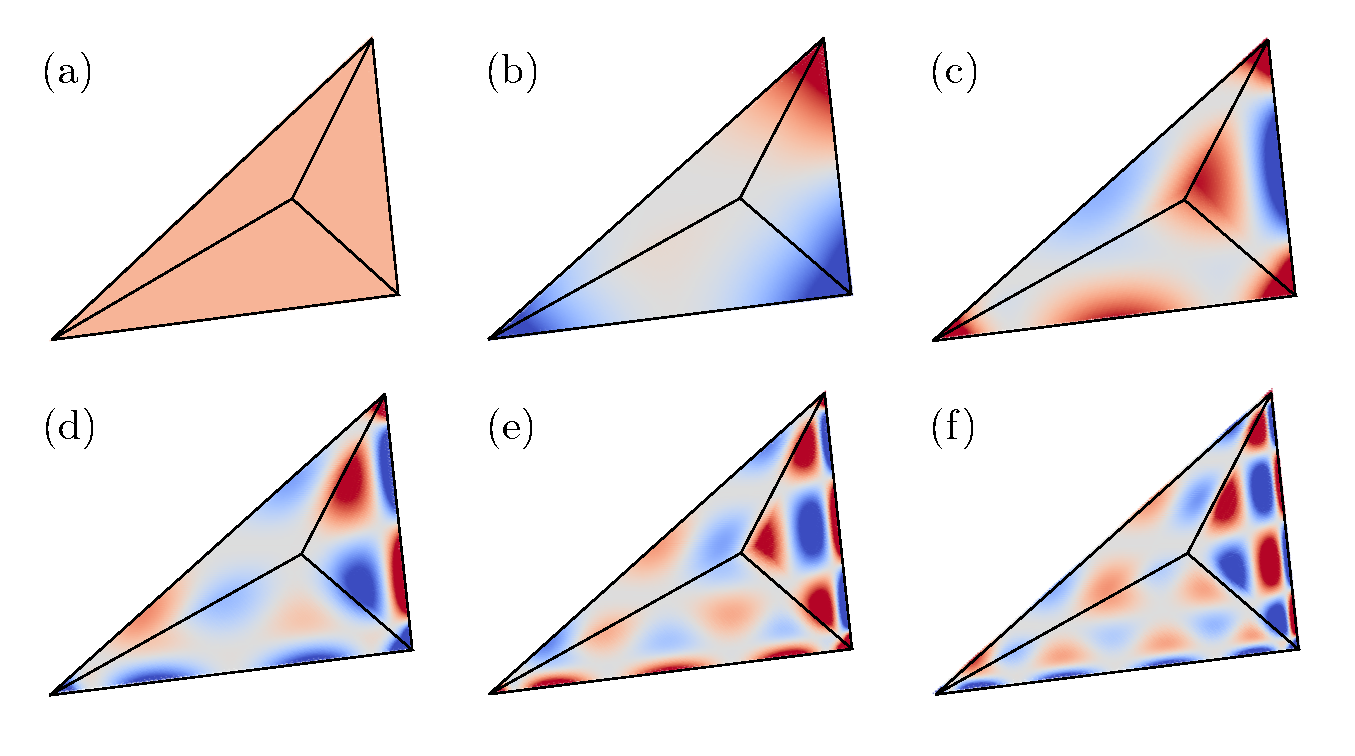
\includegraphics[width=1.0\textwidth]{legendre_modes_3D_final.pdf}
	\caption{Examples of our Legendre basis functions, evaluated on the sliced tetrapyd domain shown in Figure \ref{fig:tetrapyd}. Functions are defined as $Q_{p_1 p_2 p_3}(k_1,k_2,k_3) := P_{p_1}(k_1) P_{p_2}(k_2) P_{p_3}(k_3)$, where $P_l(k)$ are Legendre polynomials. Here we plot $p_1 = p_2 = p_3 = p$, where $p$ equals (a) $0$, (b) $1$, (c) $2$, (d) $3$, (e) $4$, and (f) $5$. A single colour map is used across the plots: red and blue correspond to $+1$ and $-1$, respectively.}	
	\label{fig:Legendre_basis_functions_3D}
\end{figure}

Let $V_{\vv{k}}$ be the subset of $\mathbb{R}^3$ representing the sliced tetrapyd. By choosing a natural inner product
\begin{align}
	\left< S_1, S_2 \right> = \int_{V_{\vv{k}}} d^3\vv{k} \;\; S_1(\vv{k}) S_2(\vv{k}), \label{eqn:tetrapyd_inner_product}
\end{align}
we restrict our attention to an $L^2$ space defined on $V_{\vv{k}}$: a vector space consisting of square-integrable functions.
\footnote{Note that the local shape function $S(k_1,k_2,k_3) = (k_1^2 / k_2 k_3 + \text{2 cyc.})$ is not in fact square-integrable due to its divergence as $k_i \rightarrow 0$. We work around this problem by prescribing a lower bound $k \ge k_\text{min}$, which is also the case in numerical calculations.}
A set of three-dimensional basis functions $Q_{\vv{p}}$ with size $N$ spans a subspace $U_{Q} \subset L^2(V_{\vv{k}})$ of dimension at most $N$.

Using this notation, expanding a given shape function $S$ with respect to a basis set $Q$ is equivalent to finding its orthogonal projection into $U_{Q}$;
\begin{align}
	&S = S^{\parallel} + S^{\perp}, \;\;\;\text{where} \\
	&S^{\parallel} \in U_Q \;\;\;\;\text{and} \;\;\; \left< S^{\perp}, Q' \right> = 0, \; \forall Q' \in U_Q.
\end{align}
As long as $\left\| S^\perp \right\| \ll \left\| S \right\|$, we may approximate
\begin{align}
	S \approx S^\parallel = \sum_{\vv{p}} \alpha_{\vv{p}} Q_{\vv{p}}.  \label{eqn:primordial_basis_projection}
\end{align}
The decomposition coefficients $\alpha$ are obtained by taking inner product with $Q_{\vv{p}}$ on both sides.
\begin{align}
	\left< S, Q_\vv{p} \right> = \left< Q_\vv{p}, Q_{\vv{p}'} \right> \alpha_{\vv{p}'}. \label{eqn:primordial_basis_expansion_SQ_and_QQ}
\end{align}
From above, we can compute $\alpha_\vv{p}$ by inverting the matrix $\Gamma_{\vv{p} \vv{p}'} = \left< Q_\vv{p}, Q_{\vv{p}'} \right>$. Alternatively, orthonormalising the basis with respect to the inner product $\left< , \right>$ turns $\Gamma$ to an identity matrix, trivialising the inversion process.

We rewrote the formalism using linear analysis language here to emphasize two aspects of our primordial basis expansion. First, even though we chose a simple inner product (\ref{eqn:tetrapyd_inner_product}) for now, the method is completely general and we may freely choose a different inner product. For example, non-unit weights $w(\vv{k})$ can be included in the integrand and/or the domain of integration may be changed. Doing so alters how we decompose shape functions in terms of our basis.

Second, we highlight the fact that basis expansion is in essence a minimisation problem with respect to the chosen inner product, which is often oblivious of late-time physics. The orthogonal projection of $S$ to subspace $U_Q$ is a point in $U_Q$ which has the minimal distance to $S$: $\left\| S - S^\parallel \right\|$ is minimised. The obtained $S^\parallel$, however, is not necessarily the best description of $S$ when we consider their late-time counterparts in $l$ space. Some errors with small norm $\left\| \Delta S \right\|$ might get enhanced when convolved with transfer functions, yielding large reduced bispectrum $\Delta b_{l_1 l_2 l_3}$. Meanwhile, sometimes large differences in $S$ are completely unobservable late-time and provide mostly identical constraints on $f_\text{NL}$.

With these points in mind, we define the following metrics to compare shape functions in primordial space;
\begin{align}
	\text{Corr}(S_1, S_2) &:= \frac{\left< S_1, S_2 \right>}{ \sqrt{ \left< S_1, S_1 \right> \left< S_2, S_2 \right> } }, \\
	\epsilon^2(S_1, S_2) &:= \frac{\left< S_1 - S_2, S_1 - S_2 \right> }{\sqrt{\left< S_1, S_1 \right> \left< S_2, S_2 \right>}}. \label{def:primordial_shape_epsilon}
\end{align}
Corr$(S_1,S_2)$ measures correlation between the two shapes and is independent of the normalisation. $\epsilon(S_1,S_2)$ is the distance between the two shapes, which reduces to $\sqrt{2 - 2\;\text{Corr}(S_1,S_2)}$ when $S_1$ and $S_2$ have equal amplitude. We use both of these values to test if our primordial basis expansion has converged to the target shape function. 

Inverting the matrix $\Gamma_{\vv{p} \vv{p}'} = \left< Q_\vv{p}, Q_{\vv{p}'} \right>$ in \eqref{eqn:primordial_basis_expansion_SQ_and_QQ} can be tricky in practice. The $p_\text{max}^3 \times p_\text{max}^3$ matrix is not only large in size for high $p_\text{max}$, but also near singular. Some of the three-dimensional mode functions $Q_\vv{p}$ become linearly dependent within tetrapyd even if they are constructed from independent modes in one dimension. The presence of such degenerate modes introduces severe numerical instability during inversion.

For our Legendre basis, we use a small trick to get around this problem. Motivated by the fact that Legendre polynomials form an orthogonal basis in one dimension, we extend the domain of integral in the inner product \eqref{eqn:tetrapyd_inner_product} to a cube containing the tetrapyd instead. Most template shape functions have an analytic form and can easily be extended in this region. As long as $\int dk \; q_p(k) q_{p'}(k) = \delta_{pp'}$, the decomposed coefficients for a given $S$ can be found by
\begin{align}
	\alpha^{(t)}_{p_1 p_2 p_3} = \int dk_1 \int dk_2 \int dk_3 \; S^{(t)}(k_1, k_2, k_3) q_{p_1}(k_1) q_{p_2}(k_2) q_{p_3}(k_3). \label{eqn:basis_expansion}
\end{align}
Note that the three-dimensional integral can now be split into three separate one-dimensional integrals in range $[k_\text{min}, k_\text{max}]$. By performing the three integrals one by one, we obtain a numerically stable algorithm that is fast and memory efficient. Decomposing a shape evaluated on $1000^3$ $k$ grid points with respect to $30^3$ Legendre basis functions only takes a few seconds in our \textsc{C} code.

After we obtain coefficients from (\ref{eqn:basis_expansion}), we evaluate the accuracy of the expansion using the inner product defined in tetrapyd because it is the only physical region where our shape function matters. Since the cube includes tetrapyd, good convergence in the cube guarantees a small error within the tetrapyd in most cases. The only exception is when the target shape function blows up outside the tetrapyd. We will see such examples in later sections.


\section{Implementation and optimisation} \label{section:implementation}

CMB bispectrum estimation is a numerically challenging task. All existing approaches exploit the separability of multi-dimensional integrals to reduce computational complexity because it is practically impossible otherwise. Planck analysis provided constraints to primordial non-Gaussianity from various bispectrum templates, but having limited computing resources was what stopped us from exploring further. Numerous shapes such as complex oscillatory models have been outside our reach, despite being theoretically well-motivated.

The \textsc{CMB-BEst} formalism significantly reduces the amount of computation needed for CMB bispectrum estimation. Obtaining the linear term $\beta^\text{lin}$ in (\ref{def:beta_linear}), however, is still prohibitively expensive unless thoroughly optimised. Performance is especially crucial here since it directly affects the breadth of models we can cover; the faster the code, the higher number of modes we can have, and so the more shapes we can expand in our basis accurately.

In this section, we provide details for various aspects of our optimisation process: algorithm design, parallel computing, and data locality improvements. The final specifications and data files used are outlined at the end.

Throughout this section, we will treat the functions of interest as discrete arrays. Our notation for indices and their limits are summarised in Table \ref{table:index_conventions}. We adopt a simple trapezoidal rule for most numerical integrals. For the $\mu$ integral in (\ref{def:gamma}), however, we use the Gauss-Legendre quadrature computed from the public code \textsc{Quadpts} \cite{Hale2013} due to the highly oscillatory and unstable nature of the integral. Multi-dimensional arrays are stored in the row-major order following the \textsc{C} convention for efficiency. We use the \textsc{Healpix} library \cite{Gorski2005healpix} for pixelisation of the sky, which includes the \textsc{Libsharp} \cite{Reinecke2013libsharp} library for Spherical Harmonic Transforms (SHTs).

\begin{table}[htbp]
	\caption{Our index conventions for discretised arrays and their sizes.}
	\centering
	\label{table:index_conventions}
	\renewcommand{\arraystretch}{1.5} 
	\begin{tabular}{m{0.1\textwidth}  m{0.1\textwidth}  m{0.7\textwidth}} \toprule
		Index & Range & Description \\
		
		\midrule
		$r$ & $[0, N_r)$ & Line-of-sight integral $r$ grid index. \\
		
		$p, p_j$ & $[0, p_\text{max})$ & Mode number. $p_j$ is a shorthand for $(p_1, p_2, p_3)$. \\
		
		$i,j$ & $[0, N_\text{sims}]$ & Map number. Index $i=0$ corresponds to the observed CMB map, while $i>0$ are for simulated Gaussian maps. \\			
		
		$n$ & $[0, N_\text{pix})$ & Map pixel number. \\ 
		
		$l,m$ & $[0, l_\text{max})$ & Spherical harmonic multipole moments. Note $-l \le m \le l$. \\
		
		$\mu$ & $[0, N_\mu)$ & Gauss-Legendre quadrature $\mu$ grid index. \\
		
		\bottomrule
	\end{tabular}
\end{table}

\subsection{Algorithm}

Our goal is to compute three key quantities: $\Gamma$ (\ref{def:gamma}), $\beta^\text{cub}$ (\ref{def:beta_cubic}), and $\beta^\text{lin}$ (\ref{def:beta_linear}). The matrix $\Gamma$ allows us to find the normalisation factor $N$ for a given theoretical template, while the two $\beta$'s provide the amplitude of $f_\text{NL}$ for each of the CMB maps and simulations used up to normalisation.

In most cases of interest, the bottleneck point of our pipeline is computing the linear term $\beta^\text{lin}$. Even though the $\Gamma$ matrix computation through (\ref{def:gamma}) grows more rapidly with the number of basis functions ($\propto p_\text{max}^6$) than the $\beta$'s ($\propto p_\text{max}^3$), it does not involve operations with high-definition maps and remains subdominant in terms of the total cost.

We dedicate this section to explaining our algorithm design for $\beta$ computation in detail. The discretised versions of (\ref{def:beta_cubic}-\ref{def:beta_linear}) are given by
\begin{align}
	\beta^\text{cub}(i, p_1,p_2,p_3) &= \sum_r \sum_n \; M(r, i, p_1, n) \cdot M(r, i, p_2, n) \cdot M(r, i, p_3, n), \\
	\beta^\text{lin}(i, p_1,p_2,p_3) &= \sum_r \sum_{j \neq i} \sum_n \; M(r, j, p_1, n) \cdot M(r, j, p_2, n) \cdot M(r, i, p_3, n).
\end{align}
The order of indices is chosen such that later calculations have optimal memory layouts. Some integral weights and factors are absorbed into arrays for brevity.

Note that the data arrays for different values of $r$ are completely independent of each other. This provides us with a natural way to distribute tasks. We compute and save contributions to $\beta$'s for each $r$ separately. The summation over $r$ is performed at the end. Therefore, throughout the rest of this chapter, we assume that $r$ is fixed and drop the $r$ dependence in the descriptions of our algorithms.

The filtered map arrays $M(i,p,n)$ are obtained as follows. A given map $i$ is first transformed into spherical harmonic coefficients $a^{(i)}(l,m)$s via SHT. We then compute $\tilde{q}_(p,l) * a(i,l,m) / C(l)$ from (\ref{def:filtered_maps}), which is fed into reverse SHT to synthesise the filtered maps.

As a rough guide to the size of each summation, we typically have $N_\text{sim} \approx 150$ simulations, $p_\text{max} = 30$ modes, and $N_\text{pix} = 50,331,648$ pixels. \footnote{This value corresponds to $N_{side} = 2048$ in Healpix. $N_\text{pix} = 12 N_{side}^2$} Considering the fact that one double-precision array of size $\sim 50$ million pixels takes about 400MB of memory space, this is indeed a task for supercomputers.

Our first and most straightforward method of computing $\beta$s is outlined in Algorithm \ref{alg:beta_first_attempt}. The computational complexity of each innermost loop is annotated on the right-hand side.

\begin{algorithm}[htbp]
	\caption{Computing $\beta$s: the na\"ive method}
	\label{alg:beta_first_attempt}
	\begin{algorithmic}[1] \State Allocate $M(i,p,n)$
		\Comment{Memory $\sim N_\text{sims} \cdot p_\text{max} \cdot N_\text{pix}$}

		\\
		\For{each map $i$}
			\For{each mode $p$}
			\Comment{$O(N_\text{sims} \cdot p_\text{max} \cdot N_\text{pix}^{3/2})$}
				\State \textbf{compute} $M(i,p,n)$ by SHT
			\EndFor
		\EndFor \Comment{$M(i,p,n)$ ready}
		\\
		
		\For{each map $i$}
			\For{each set of modes $(p_1,p_2,p_3)$}
				\For{each pixel $n$}
				\Comment{$O(N_\text{sims} \cdot p_\text{max}^3 \cdot N_\text{pix})$}
					\State $\beta^\text{cub}(i, p_1, p_2, p_3) \pluseq M(i,p_1,n) \cdot M(i,p_2,n) \cdot M(i,p_3,n)$
				\EndFor
			\EndFor
		\EndFor

		\\	
		\For{each map $i$}
			\For{each map $j \neq i$}
				\For{each set of modes $(p_1,p_2,p_3)$}
					\For{each pixel $n$}
					\Comment{$O(N_\text{sims}^2 \cdot p_\text{max}^3 \cdot N_\text{pix})$}
						\State $\beta^\text{lin}(i, p_1, p_2, p_3) \pluseq M(j,p_1,n) \cdot M(j,p_2,n) \cdot M(i,p_3,n)$
					\EndFor
				\EndFor
			\EndFor
		\EndFor

	\end{algorithmic}
\end{algorithm}

Here, we first obtain the filtered maps $M(i,p,n)$ via SHT for each map and mode. The full results are stored in memory. Next, we iterate through each map and set of modes $(p_1, p_2, p_3)$ and sum over each of the map pixels to obtain $\beta^\text{cub}$ and $\beta^\text{lin}$. Symmetries in the indices are respected; we only loop over $(p_1,p_2,p_3)$ satisfying $p_1\ge p_2$ for the linear terms, and $p_1\ge p_2\ge p_3$ for the cubic ones.

SHT typically scales as $\propto l_\text{max}^3$, where $l_\text{max}$ is the maximum degree of spherical harmonic functions used. The total number of pixels $N_\text{pix}$ grows $\propto l_\text{max}^2$ when chosen appropriately for resolution, hence the SHT costs $O(N_\text{sims}\cdot p_\text{max} \cdot N_\text{pix}^{3/2})$. The most expensive part of this algorithm is still the loop where we calculate the linear term, which scales as $O(N_\text{sims}^2 \cdot p_\text{max}^3 \cdot N_\text{pix})$.

Our first major optimisation comes from the observation that we may swap the order of summations to reduce the computation. By precomputing $C(p_1, p_2, n) = \sum_j M(j,p_1,n) \cdot M(j,p_2,n)$, we require one fewer loop over maps for $\beta^\text{lin}$, leading to a factor of $N_\text{sims}\sim150$ improvement. Algorithm \ref{alg:beta_second_attempt} shows a pseudocode for this method.

\begin{algorithm}[htbp]
	\caption{Computing $\beta$s: optimised for computation}
	\label{alg:beta_second_attempt}
	\begin{algorithmic}[1] \State Allocate $M(i,p,n)$ \Comment{Memory $\sim N_\text{sims} \cdot p_\text{max} \cdot N_\text{pix}$}
		\State Allocate $C(p_1,p_2,n)$ \Comment{Memory $\sim p_\text{max}^2 \cdot N_\text{pix}$}
		\\
		\For{each map $i$}
			\For{each mode $p$}
				\Comment{$O(N_\text{sims} \cdot p_\text{max} \cdot N_\text{pix}^{3/2})$}
				\State \textbf{compute} $M(i,p,n)$ by SHT
			\EndFor
		\EndFor \Comment{$M(i,p,n)$ ready}
		\\
		\For{each map $j$}
			\For{each pair of modes $(p_1,p_2)$}
				\For{each pixel $n$}
					\Comment{$O(N_\text{sims} \cdot p_\text{max}^2 \cdot N_\text{pix})$}
					\State $C(p_1,p_2,n) \pluseq M(j,p_1,n) \cdot M(j,p_2,n)$
				\EndFor
			\EndFor
		\EndFor \Comment{$C(p_1,p_2,n)$ ready}
		\\
		\For{each map $i$}
			\For{each set of modes $(p_1,p_2,p_3)$}
				\For{each pixel $n$}
					\Comment{$O(N_\text{sims} \cdot p_\text{max}^3 \cdot N_\text{pix})$}
					\State $\beta^\text{cub}(i, p_1, p_2, p_3) \pluseq M(i, p_1, n) \cdot M(i, p_2, n) \cdot M(i, p_3, n)$
					\State $\beta^\text{lin}(i, p_1, p_2, p_3) \pluseq C(p_1, p_2, n) \cdot M(i, p_3, n)$
				\EndFor
			\EndFor
		\EndFor
	\end{algorithmic}
\end{algorithm}

Note that the resulting sum of $\beta^\text{lin}$ includes an unwanted contribution from the case where $j=i$, since $C(p_1,p_2,n)$ is obtained by summing over all maps. Thankfully, this extra contribution is exactly equal to the cubic term. We just have to subtract $\beta^\text{cub}$ from the total sum to get the correct value of $\beta^\text{lin}$.

We shaved off a whole loop at the cost of extra memory usage. For our purposes $N_\text{sims} \sim 150 > p_\text{max} = 30$, so the additional space required for $C(p_1,p_2,n)$ is relatively small compared to $M(i,p,n)$. The symmetry in $p_1$ and $p_2$ also means that we only need to store $p_\text{max}(p_\text{max}+1)/2$ maps instead of $p_\text{max}^2$ for $C$.

Our next challenge is the amount of memory required to save $M(i,p,n)$. For the parameters mentioned above, this is $\approx 1.8$TB, which is quite significant. Although it is not impossible to find supercomputing systems which can accommodate such large arrays, reducing the memory usage would be highly beneficial. We seek to achieve this whilst keeping the overall computational complexity to be $O(N_\text{sims} \cdot p_\text{max}^3 \cdot N_\text{pix})$ as before.

We observe that most summations are done for a single map $i$. The array $C(p_1,p_2,n)$ is required to be computed before the main loop for $\beta^\text{lin}$, but otherwise there are no `mixing' between the maps. We exploited this fact to develop Algorithm \ref{alg:beta_third_attempt}.

\begin{algorithm}[htbp]
	\caption{Computing $\beta$s: fast and memory efficient}
	\label{alg:beta_third_attempt}
	\begin{algorithmic}[1] \State Allocate $m(p,n)$ \Comment{Memory $\sim p_\text{max} \cdot N_\text{pix}$}
		\State Allocate $C(p_1,p_2,n)$ \Comment{Memory $\sim p_\text{max}^2 \cdot N_\text{pix}$}
		\\
		\For{each map $i$}
			\For{each mode $p$}
				\Comment{$O(N_\text{sims} \cdot p_\text{max} \cdot N_\text{pix}^{3/2})$}
				\State \textbf{compute} $M(i,p,n)$ by SHT and store in $m(p,n)$
			\EndFor
			\\
			\For{each pair of modes $(p_1,p_2)$}
				\For{each pixel $n$}
				\Comment{$O(N_\text{sims} \cdot p_\text{max}^2 \cdot N_\text{pix})$}
					\State $C(p_1,p_2,n) \pluseq m(p_1,n) \cdot m(p_2,n)$
				\EndFor
			\EndFor
		\EndFor
		\Comment{$C(p_1,p_2,n)$ ready}
		\\
		\For{each map $i$}
			\For{each of mode $p$}
				\Comment{$O(N_\text{sims} \cdot p_\text{max} \cdot N_\text{pix}^{3/2})$}
				\State \textbf{compute} $M(i,p,n)$ by SHT and store in $m(p,n)$
			\EndFor
			\\
			\For{each set of modes $(p_1,p_2,p_3)$}		\label{alg:thrid_attempt_main_loop}	
				\For{each pixel $n$}
					\Comment{$O(N_\text{sims} \cdot p_\text{max}^3 \cdot N_\text{pix})$}	
					\State $\beta^\text{cub}(i, p_1, p_2, p_3) \pluseq m(p_1,n) \cdot m(p_2,n) \cdot m(p_3,n)$
					\State $\beta^\text{lin}(i, p_1, p_2, p_3) \pluseq C(p_1, p_2, n) \cdot m( p_3, n)$
				\EndFor
			\EndFor
		\EndFor
	\end{algorithmic}
\end{algorithm}

Algorithm \ref{alg:beta_third_attempt} dramatically reduces the amount of memory required, at the cost of doubling the SHTs for computing $M(i,p,n)$s. The first time through, SHT results from each map are used to find $C(p_1,p_2,n)$. After a full loop over maps we have $C(p_1,p_2,n)$ ready, another set of SHTs for each map allows us to obtain the $\beta$'s.

SHTs have a subdominant contribution to the total computation time even after becoming doubled in number. One of the main strengths of Algorithm \ref{alg:beta_third_attempt} is that both the memory and computation time scale linearly with the number of simulations used, $N_\text{sims}$. In the future when a larger number of Gaussian simulations are required to acquire a more accurate estimate of the linear term, it is straightforward to adapt our method accordingly.

We choose Algorithm \ref{alg:beta_third_attempt} to be our main method of computing $\beta$'s for \textsc{CMB-BEst}.

\subsection{Parallel computing}



In order to fully benefit from modern computer architecture, parallel computing is essential. In this section, we outline how \textsc{CMB-BEst} was parallelised for optimal performance on supercomputers.

Following \cite{Jeffers2016intel}, we discuss parallelisation at three different levels: domain, thread, and data. They mostly correspond to nodes, cores, and registers in modern computer clusters. Each level has distinct characteristics which make them ideal for different parallelisation techniques. We make full use of each level in our methodology.

\textit{Domain} parallelism refers to dividing the task into many domains where each domain entails heavy computation while having limited data communication between them. Since the domains are largely independent, Message Passing Interface (MPI) \cite{Gropp1999MPI} is a suitable tool for parallelisation. MPI is a communication protocol where many instances (`ranks') of the same code may transfer data while running separately from each other \. A perfect example of domain parallelism in \textsc{CMB-BEst} would be our line-of-sight integration over $r$. Almost no data is shared between different $r$s, despite the heavy computational cost from map operations within each domain. \textsc{CMB-BEst} therefore scales well with the number of MPI ranks and requires minimal effort to parallelise using MPI.

\textit{Thread} parallelism opportunities arise when there are many independent computational tasks on a single set of data. Most modern supercomputers use multi-core processors. Each core, or processing unit, can run one or more threads, executing instructions independently from each other while sharing memory space. Note that MPI would not be as effective here due to a large amount of data sharing needed; ranks have to either continuously communicate with each other, or store individual copies of the data. This type of parallelism is extremely common in many applications, including SHTs and map integrations in \textsc{CMB-BEst}. Open Multi-Processing (OpenMP) \cite{Dagum1998openmp} is one of the most popular implementations of multi-threading publicly available. We utilise the \textsc{C} OpenMP interface in our code. 

\textit{Data} parallelism applies when the same arithmetic operations are applied to multiple data items, ideally adjacent in memory space. This type of parallel processing is called SIMD: Single Instruction, Multiple Data. Many procedures involving large arrays fall into this category. We use Advanced Vector Extensions (AVX) supported by Intel processors to exploit data parallelism in \textsc{CMB-BEst}, especially for the operations involving large (filtered) map arrays. In particular, Intel's Xeon Phi series implement AVX-512, where 512-bit registers hold up to 8 double-precision floating numbers \cite{Jeffers2016intel}. A single instruction can be applied to all of them at once in a single clock cycle, providing a major boost to the computation speed. We explicitly align large arrays in memory for optimal vectorisation performance.

Table \ref{table:three_levels_of_parallelism} summarises the discussions in this section.

\begin{table}[h]
	\caption{Three levels of parallelism utilised in \textsc{CMB-BEst}. The levels and characteristics are chosen based on \cite{Jeffers2016intel}.}
	\centering
	\label{table:three_levels_of_parallelism}
	\renewcommand{\arraystretch}{1.5} 
	\begin{tabular}{m{0.12\textwidth}   m{0.35\textwidth}   m{0.15\textwidth}   m{0.3\textwidth}} \toprule
		 & Characteristics & Methods & Utilisation \\
		
		\midrule
		Domain \newline Parallelism &
		\begin{itemize}[leftmargin=*]
			\item Limited data communication between domains
			\item Heavy computation within the domain
		\end{itemize} &
		MPI &
		\begin{itemize}[leftmargin=*]
			\item Line of sight $r$ integration split into independent tasks
		\end{itemize}  \\
	
		\midrule
		Thread \newline Parallelism &
		\begin{itemize}[leftmargin=*]
			\item Data sharing between threads
			\item High proportion of independent tasks
		\end{itemize} &
		OpenMP &
		\begin{itemize}[leftmargin=*]
			\item SHT
			\item Map patches divided across threads
		\end{itemize}  \\	
	
		\midrule
		Data \newline Parallelism &
		\begin{itemize}[leftmargin=*]
			\item Same operation applied to multiple data items
		\end{itemize} &
		SIMD &
		\begin{itemize}[leftmargin=*]
			\item Map pixel integration vectorised using AVX-512
			\item Data vectors explicitly aligned in memory for optimal performance 
		\end{itemize} \\	
			
		\bottomrule
	\end{tabular}
\end{table}

\subsection{Data locality}

We implemented Algorithm \ref{alg:beta_third_attempt} and profiled it using the Intel VTune Amplifier. Our program was found to be memory-bound, which means that its speed is limited mainly by the amount of memory available and the speed of memory access. The CPU speed, rate of the file I/O, and MPI communication all have subdominant contributions in comparison. This is somewhat expected since our method deals with large map arrays. The number of operations on each data element is small compared to the size of data, causing the CPUs to be `starved' for data to work on most of the time. Our final set of optimisation focusses on improving memory access patterns.

CPUs of most modern computers contain a small amount of memory attached to them called \textit{cache}. Recently used data and instructions are stored in cache memory so that reusing them is more efficient; accessing them is much faster than loading from the main, larger memory often shared with other CPUs. A cache is often divided into multiple levels. The smallest and fastest is the L1 cache, which is the first level a CPU checks for data. When the required data is not stored in the L1 cache, a \textit{cache miss} occurs. The system then has to look further down the cache levels to fetch the wanted data, incurring a large time loss. It is therefore crucial to reuse data as many times as possible before it is lost from the cache.

Furthermore, the cache `caches' memory locations in units of cache lines, or chunks of memory containing multiple data elements. Accessing memory locally therefore significantly increases the chance of cache hits, boosting overall performance. Array operations, for example, are optimised when they are stored in consecutive memory locations due to this fact.

\textsc{CMB-BEst} has been modified in two ways to improve data locality and memory performance. The first one was simple yet effective; we made sure to initialise large arrays within the same OpenMP construct as the main computation loop. This guarantees the physical memory of array elements to be allocated near the cores where they are going to be used. Memory access during the main computation loop is therefore much faster than it would be otherwise. Systems with non-uniform memory access (NUMA) especially benefit from this method. For \textsc{CMB-BEst}, we gained a two times speed-up compared to when a single master thread initialised the entire array.

The second optimisation centres around \textit{cache blocking}, a technique used to maximise data reuse. Let us focus on the main computation loop in Algorithm \ref{alg:beta_third_attempt}:

\begin{algorithmic}
	\For{each set of modes $(p_1,p_2,p_3)$}
		\For{each pixel $n$}
			\State $\beta^\text{cub}(i, p_1, p_2, p_3) \pluseq m(p_1,n) \cdot m(p_2,n) \cdot m(p_3,n)$
			\State $\beta^\text{lin}(i, p_1, p_2, p_3) \pluseq C(p_1, p_2, n) \cdot m( p_3, n)$
		\EndFor
	\EndFor
\end{algorithmic}

In every loop over the set of modes $(p_1, p_2, p_3)$, four large arrays are read from memory: $m(p_1,\cdot)$, $m(p_2,\cdot)$, $m(p_3,\cdot)$, and $C(p_1, p_2, \cdot)$. Each of them takes up around 400MB of memory. Since their size is greater than the cache storage capacity, data in front of them are gone from the cache by the time a loop over $n$ completes. All four arrays will then have to be loaded from the main memory again when the next iteration starts.

Suppose that the map arrays had smaller sizes and all of them fit in one of the cache levels instead. After one loop iteration over $n$ for $(p_1, p_2, p_3)$, the arrays now remain in the cache. Then the next loop on $(p_1, p_2, p_3+1)$ begins, and the arrays $m(p_1,\cdot)$, $m(p_2,\cdot)$, and $C(p_1,p_2,\cdot)$ are required again for computation. They can now be accessed from the cache, which saves a significant amount of time. We see that each data element is reused multiple times before being discarded from the cache in this case.

Motivated by these facts, we divide the map array into equally sized blocks so that each patch can now fit inside the cache memory. We restructure the loop as follows.

\begin{algorithmic}
	\For{each block $b$}
		\For{each set of modes $(p_1,p_2,p_3)$}
			\For{each pixel $n'$ in block}
				\State $\beta^\text{cub}(i, p_1, p_2, p_3) \pluseq m(p_1,n') \cdot m(p_2,n') \cdot m(p_3,n')$
				\State $\beta^\text{lin}(i, p_1, p_2, p_3) \pluseq C(p_1, p_2, n') \cdot m( p_3, n')$
			\EndFor
		\EndFor
	\EndFor
\end{algorithmic}

New pixel numbers are calculated as $n' = B \cdot b + n$, where $B$ is the size of each block and $0 \le n < B$. We have not changed the total number of arithmetic operations required, so the computational complexity remains constant. Meanwhile, data locality within each block is greatly improved, as each of the blocked arrays is now small enough to fit in the cache. Each data element is accessed in closer succession temporarily as well.

One caveat here is that having too many blocks may degrade the overall performance. There exists a non-negligible overhead coming from an extra \textit{for} loop and the OpenMP construct used over $n'$. The block size divided by the number of cores should not be smaller than the size of cache lines either. The optimal size of cache blocks depends on the memory architecture of the processor used. This often needs to be found empirically.

Figure (\ref{fig:cache_block_optimisation}) shows how the runtime of a small test code varies with the number of cache blocks used. The code was run on the Intel Gold 6154 processor, which is an 18-core high-performance chip with total L1, L2, and L3 cache memory sizes of 1.125MiB, 18MiB, and 24.74MiB, respectively \cite{intel_data_sheet}. Even though some parameters such as $N_\text{sims}$ are tuned down for faster testing, this is representative of the full computation.

\begin{figure}[htbp!] 
	\centering    
	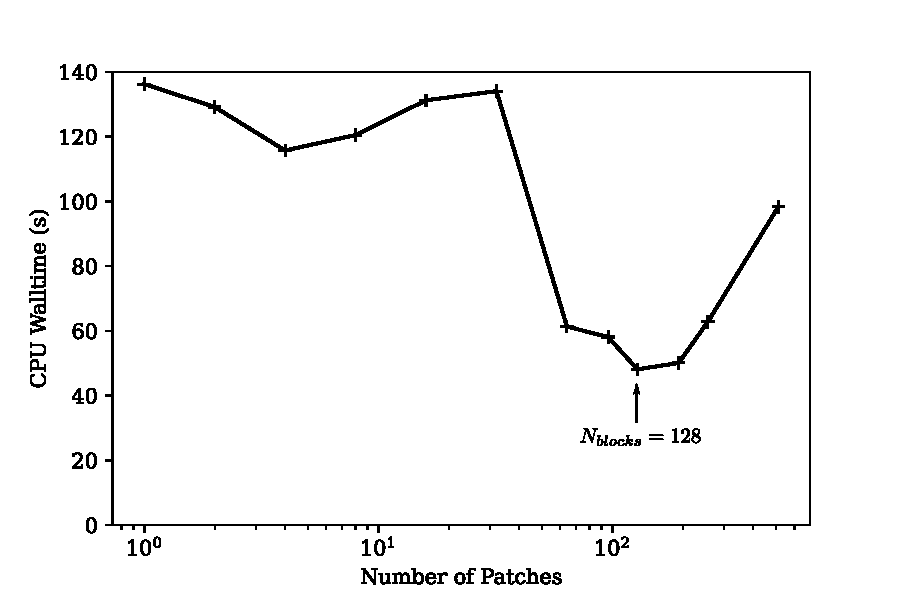
\includegraphics[width=0.8\textwidth]{cache_block_optimisation_annotated.pdf}
	\caption[Cache block optimisation]{Cache block optimisation. The total wall time of a test code for computing $\beta$s was measured while varying the number of cache blocks used. Having 128 blocks is optimal for the 18-core Intel Gold 6154 processor.}
	\label{fig:cache_block_optimisation}
\end{figure}

We find a significant improvement in performance moving from 32 to 48 blocks when the block size drops from 12MiB to 8MiB. This is precisely when three blocks are allowed to fit in the L3 cache (24.7MiB) at the same time. Improved data locality dramatically reduces time spent on memory access as we expected. The optimal number of blocks was found to be 128; each segment contains about 400,000 elements and takes up 3MiB of memory, which is 1/6 and 1/8 of L2 and L3 cache size, respectively. We gain roughly three times speed-up compared to the original code without cache blocking.

Algorithm \ref{alg:beta_final_algorithm} summarises our final implementation of $\beta$ computation code, now with cache blocking and OpenMP construct indicators.

\begin{algorithm}[htbp]
	\caption{Computing $\beta$s: our final implementation}
	\label{alg:beta_final_algorithm}
	\begin{algorithmic}[1] \State Allocate $m(p,n)$ 
		\State Allocate $C(p_1,p_2,n)$ 
		\\\Comment{Both initialised within OpenMP construct over $n$}

		\For{each map $i$}
		\For{each mode $p$}
		\State \textbf{compute} $M(i,p,n)$ by SHT and store in $m(p,n)$
		\Comment{OpenMP within SHT}
		\EndFor
		\\
		\For{each block $b$}
		\For{each pair of modes $(p_1,p_2)$}
		\For{each pixel $n'$ in block}
		\Comment{OpenMP \textit{for} construct}
		\State $C(p_1,p_2,n') \pluseq m(p_1,n') \cdot m(p_2,n')$
		\EndFor
		\EndFor
		\EndFor
		\EndFor
		\Comment{$C(p_1,p_2,n)$ ready}
		\\
		\For{each map $i$}
		\For{each of mode $p$}
		\State \textbf{compute} $M(i,p,n)$ by SHT and store in $m(p,n)$
		\Comment{OpenMP within SHT}
		\EndFor
		\\
		\For{each block $b$}
		\For{each set of modes $(p_1,p_2,p_3)$}		
		\For{each pixel $n'$ in block}
		\Comment{OpenMP \textit{for} construct}
		\State $\beta^\text{cub}(i, p_1, p_2, p_3) \pluseq m(p_1,n') \cdot m(p_2,n') \cdot m(p_3,n')$
		\State $\beta^\text{lin}(i, p_1, p_2, p_3) \pluseq C(p_1, p_2, n') \cdot m( p_3, n')$
		\EndFor
		\EndFor
		\EndFor
		\EndFor
	\end{algorithmic}
\end{algorithm}

\section{Validation} \label{section:validation}

CMB bispectrum estimation is not only computationally challenging but also prone to numerical instabilities unless implemented carefully. We invested a considerable amount of time after the development of \textsc{CMB-BEst} validating various aspects of the code. We highlight some of our validation efforts in this section, checking consistency within the program itself (section \ref{section:internal_consistency}) and against existing code such as Modal \cite{Fergusson2012} (section \ref{section:consistency_with_Planck}).

\subsection{Internal consistency checks} \label{section:internal_consistency}

\textsc{CMB-BEst} is a general code where one can freely choose a set of basis functions. Three of our main options are the `KSW' basis (\ref{eqn:KSW_basis}), `Legendre' basis (\ref{eqn:Legendre_basis_no_inv_k}, augmented with $q(k)=k^{n_\text{s}-2}$) as discussed previously in Section \ref{section:basis_functions}, and Fourier basis (\ref{eqn:Fourier_basis}). Both KSW and Legendre basis sets can cover the standard templates: local, equilateral, and orthogonal (see e.g., \cite{PlanckCollaboration2013} for definitions). The KSW basis provides an exact form for the three templates by choosing appropriate powers of $k$ as its basis elements. On the other hand, the templates are expanded in terms of separable Legendre polynomials up to some fixed degree $p_\text{max}$ for the Legendre basis. As long as $p_\text{max}$ is sufficiently large, most smooth bispectrum shapes can be represented accurately. 

Our first consistency check is shown in Figure \ref{fig:map_by_map_Legendre_KSW}, where we compare the $f_\text{NL}$ estimates from the Planck 2018 CMB map and 140 full focal plane (FFP10) realistic Gaussian simulations \cite{PlanckCollaboration2015simulations}. We use CMB maps obtained through the SMICA component separation method \cite{Cardoso2008component, PlanckCollaboration2013ComponentSeparation}. On the left-hand side are scatter plots of $f_\text{NL}$ values obtained using each of the two basis sets. In an ideal case where the two estimates are identical for every test map, all the points would lie on a straight line given by $y=x$. Drawn in dashed red line is the best linear fit to the data. Its slope, intercept, and the $R$-squared value are annotated below. On the right is a more detailed plot of the computed $f_\text{NL}$ for each map.

\begin{figure}[htbp!] 
	\centering 
	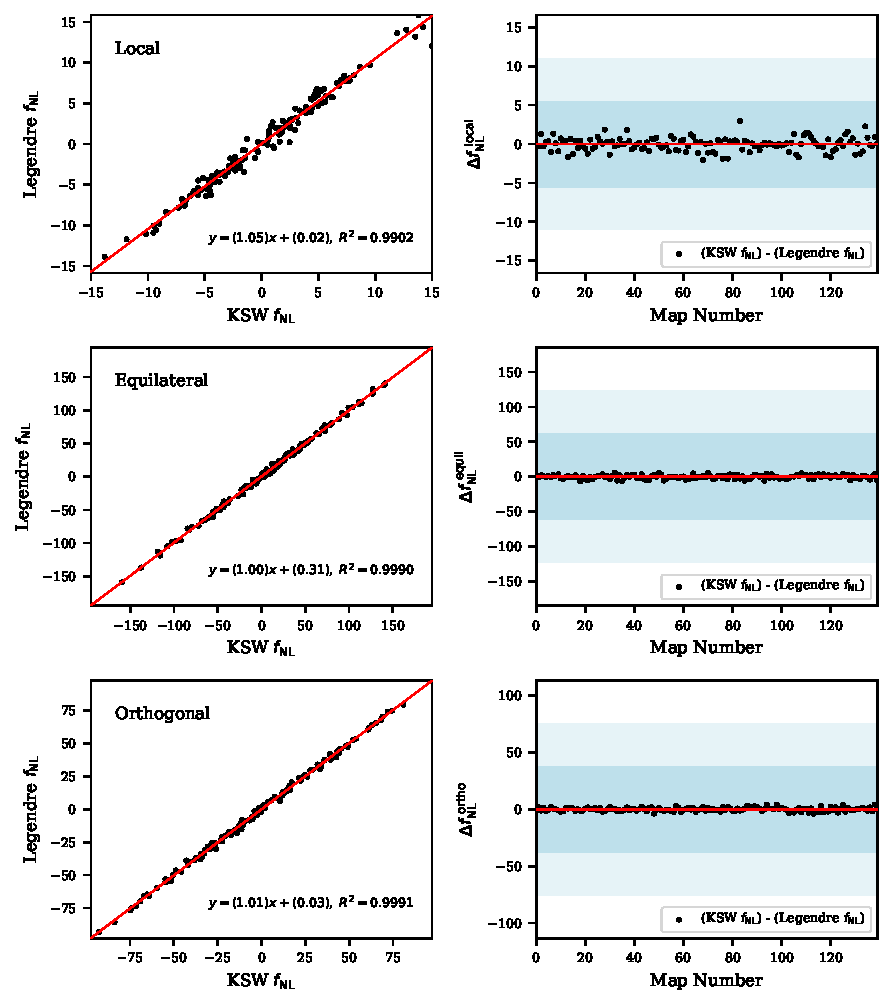
\includegraphics{map_by_map_Legendre_KSW.pdf}
	\caption{A map-by-map comparison of the $f_\text{NL}$ estimates evaluated using the KSW and Legendre basis sets for three standard templates. The Planck 2018 CMB map and 140 FFP10 simulations have been used, each representing a single point on the scatter plot (left). Details of the linear best-fit to data (red) are annotated below. Shown on the right-hand side are plots of the differences in the $f_\text{NL}$ values for each map, together with the $1\sigma$ and $2\sigma$ intervals shaded in blue. In the ideal case where the two basis sets yield identical results, we should see all the points lie on the line $y=x$ for the left plot and $y=0$ for the right plot. For more information on each of the three theoretical templates used, see e.g., \cite{PlanckCollaboration2013}.}
	\label{fig:map_by_map_Legendre_KSW}
\end{figure}

We see that results from the two different sets of basis are in good agreement. The $R$-squared value of the linear fit is greater than $0.99$ for Local, and $0.999$ for Equilateral and Orthogonal shapes. The intercept and sample mean are also near zero. We do not find any systematic discrepancies across the shapes from individual map estimates either.

The fact that the results from the KSW and Legendre basis are consistent validates multiple aspects of our pipeline. First of all, we can deduce that the Legendre basis expansion (\ref{eqn:basis_expansion}) accurately represents the bispectrum shapes of interest, especially since the KSW basis is designed to be exact for the three standard shapes. Having $p_\text{max}=30$ modes is more than sufficient to achieve sub-percent accuracy. Figure \ref{fig:map_by_map_Legendre_30_29} explicitly compares results obtained from Legendre bases with $p_\text{max}=29$ and $30$ while keeping everything else the same. The two results show close agreement; the largest of the errors is less than $O(10^{-5})$. This further confirms that our expansion using Legendre polynomials has completely converged.

\begin{figure}[htbp!] 
	\centering    
	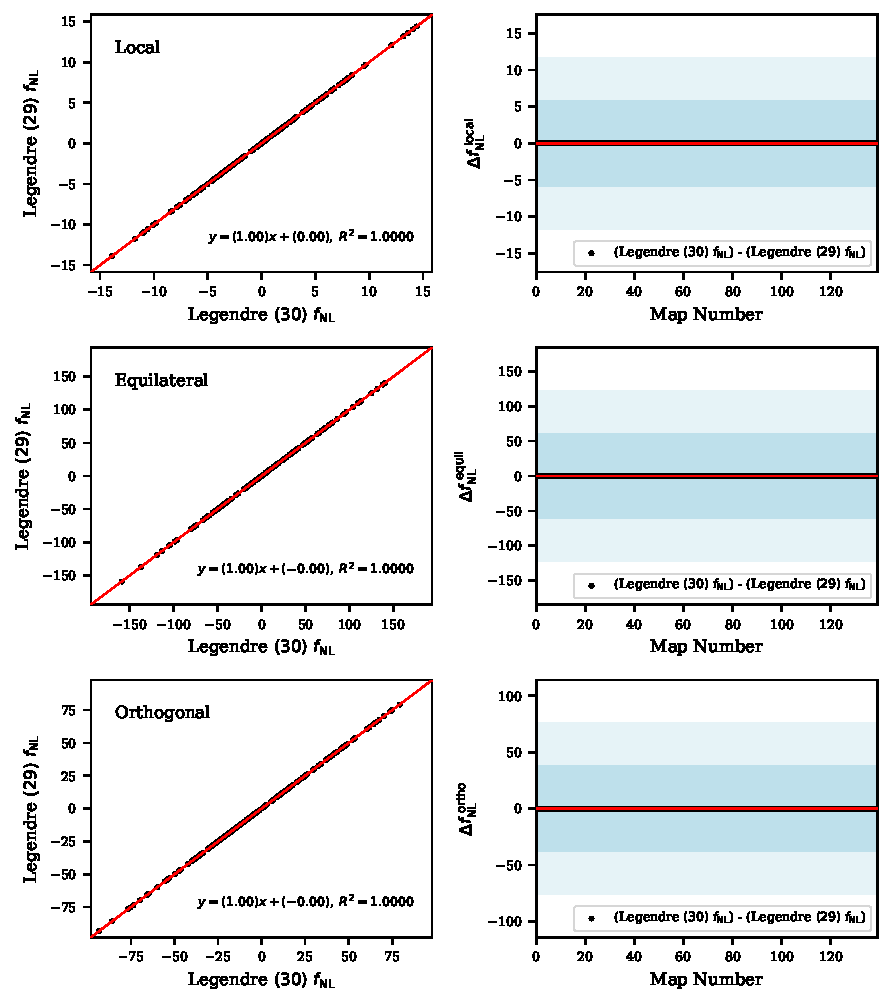
\includegraphics{map_by_map_Legendre_30_29.pdf}
	\caption{A map-by-map comparison of the $f_\text{NL}$ estimates for three standard templates evaluated using the Legendre basis with different numbers of modes: $p_\text{max}=29$ and $30$. The two results agree with errors less than $O(10^{-5})$, as can be seen from the scatter plots (left) and the map-by-map residual plots (right). Shaded in blue are the $1\sigma$ and $2\sigma$ levels of the $f_\text{NL}$ estimator. This confirms that our expansion using Legendre polynomials has completely converged for these bispectrum shapes.}
	\label{fig:map_by_map_Legendre_30_29}
\end{figure}

Secondly, we validated the accuracy of the linear term and lensing-ISW bias calculations through the sample mean of $f_\text{NL}$ estimates from lensed simulations. When we exclude either of the two, we find the sample mean to be far from zero. The error is especially large for the local template. The linear term accounts for the anisotropy introduced by masking parts of the observed sky. The squeezed limit contribution to the bispectrum comes from couplings between a pair of small-scale modes and a large-scale one, making it more susceptible to bias from partial coverage. The presence of sky masks therefore offsets the $f_\text{NL}$ estimates from the local shape which has a large squeezed limit. Lensing-ISW bias is also the largest in squeezed configurations and affects Local $f_\text{NL}$. The fact that our lensed Gaussian simulations have $f_\text{NL}$s fluctuating around $0$ validates our bias subtractions.

Lastly, we check that \textsc{CMB-BEst} accurately preserves the optimality of the CMB bispectrum estimator. In the weak non-Gaussian limit, the estimator (\ref{eqn:bispectrum_estimator_standard}) saturates the Cramer-Rao bound. Its expected variance is the lowest amongst all possible unbiased bispectrum estimators of $f_\text{NL}$. Heuristically speaking, the estimator extracts as much information about non-Gaussianity as possible from the CMB bispectrum. As we discussed in Chapter \ref{chapter:CMB_state-4_forecast}, this bound only depends on the Fisher information determined from normalisation; $Var[\hat{f}_\text{NL}]=F^{-1}=6/N$. We refer to this value as the \textit{theoretical} variance (the best possible from theory). Meanwhile, individual $f_\text{NL}$ estimates from simulated maps and independent and normally distributed. Sample variance obtained from $N_\text{sims}$ simulations should therefore approach the theoretical variance as $N_\text{sims}\rightarrow\infty$. Table \ref{table:trio_sample_and_theory_variances} summarises calculated values of the two types of variances discussed.

\begin{table}[h]
	\caption{Comparison of the sample and theoretical variances obtained from $f_\text{NL}$ estimates of standard shapes, computed using each of the KSW and Legendre basis sets. Sample variances are within $1\sigma$ of theoretical values assuming that the 140 individual $f_\text{NL}$'s from simulated maps are normally distributed. This is statistically consistent with the optimality of our bispectrum estimator.}
	\centering
	\label{table:trio_sample_and_theory_variances}
	\renewcommand{\arraystretch}{1.5} 
	\begin{tabular}{llccc}
		\toprule
		Template & Basis & Sample Variance &  Theoretical Variance &  (Sample)/(Theory) \\
		\midrule
		\multirow{2}{*}{Local} & KSW &  5.5 &       5.3 &               1.04 \\
		& Legendre &             5.9 &                  5.7 &               1.04 \\
		\multirow{2}{*}{Equilateral} & KSW &            61.2 &                 67.7 &               0.90 \\
		& Legendre &            61.7 &                 67.7 &               0.91 \\
		\multirow{2}{*}{Orthogonal} & KSW &            37.7 &                 33.7 &               1.12 \\
		& Legendre &            38.0 &                 33.9 &               1.12 \\
		\bottomrule
	\end{tabular}
\end{table}

Note that the numbers do not match up exactly between sample and theoretical variances, and the results for equilateral template appear to be more optimal than the theory allows. This is because the sample variance $\hat{S}^2 = (\sum_i (f^{(i)}_\text{NL})^2 )/N_\text{sims}$ follows a chi-squared distribution with $N_\text{sims}-1$ degrees of freedom under our assumptions. The standard deviation corresponding to the (normalised) distribution equals $\sqrt{2/(N_\text{sims}-1)}$, which is $\approx 0.12$ for $N_\text{sims}=140$. It is therefore not surprising to see our sample variances differ by up to $12\%$ from the theoretical ones. 

We performed further checks to ensure that this discrepancy is due to statistical fluctuations rather than systematic errors. The ratio between the sample and theoretical variances remained nearly constant across the KSW and Legendre basis from \textsc{CMB-BEst}, as well as Planck's Modal pipeline on the same set of simulated maps. Meanwhile, sample variances evaluated from independent sets of simulations do fluctuate around the theoretical value. A closer check has been done for each of the mode sets $(p_1,p_2,p_3)$ in the Legendre basis. The decomposition coefficient $\alpha$ is set to be 1 at $(p_1,p_2,p_3)$ and its permutations, and then vanishing everywhere else. Substituting into \eqref{eqn:fNL_from_betas} and \eqref{eqn:normlisation_from_gamma}, we get
\begin{align}
	f_\text{NL}^{(i)} &= \frac{1}{N} \left[ \left( \beta^{\textrm{cub},(i)}_{p_1 p_2 p_3} - 3 \beta^{\textrm{lin},(i)}_{p_1 p_2 p_3} \right) + \text{5 cyc.} \right], \\
	N &= 6\left( \Gamma_{p_1 p_2 p_3, p_1 p_2 p_3} + \Gamma_{p_1 p_2 p_3, p_1 p_3 p_2} + \cdots + \Gamma_{p_1 p_2 p_3, p_3 p_2 p_1} \right).
\end{align}
Here we assumed that $p_1,p_2,p_3$ are distinct for convenience. Corresponding sample and theoretical variances have been compared for each of the modes. Overall, they are found to be statistically consistent as before.



While Figure \ref{fig:map_by_map_Legendre_KSW} shows excellent agreement between results from the KSW and Legendre basis sets overall, there are small but noticeable scatters in the plot for the local shape. The slope of linear best fit is also slightly above 1, meaning that $f_\text{NL}$ estimates from the Legendre routine tend to vary 5\% more than the KSW ones. A larger variance means less information extracted. Our first hypothesis was that the Legendre polynomials are losing a small fraction of information from the CMB due to their fixed $k$ range in their definition ($\ref{eqn:Legendre_basis_no_inv_k}$). We test this by increasing the range by changing $k_\text{max}/k_\text{min} = 1000$ to $2000$. The results are shown in Figure \ref{fig:map_by_map_Legendre_KSW_k_ratio_2000}.

\begin{figure}[htbp!] 
	\centering    
	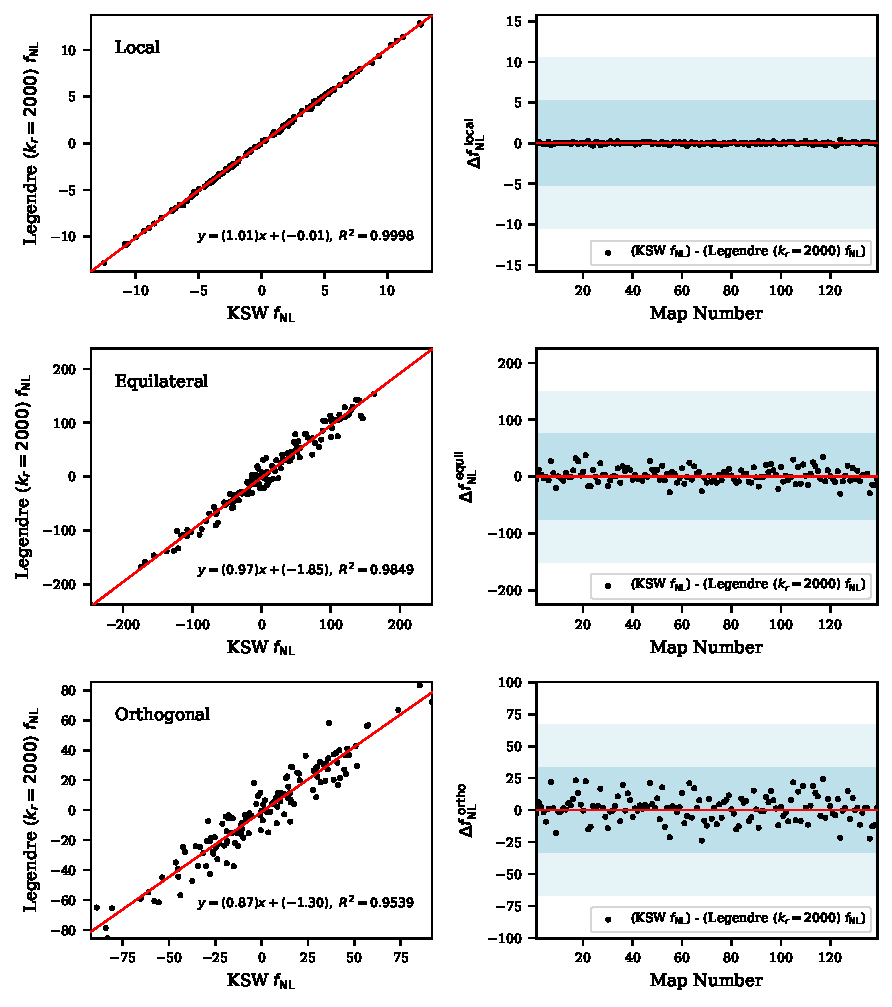
\includegraphics{map_by_map_Legendre_KSW_k_ratio_2000.pdf}
	\caption{A map-by-map comparison of the $f_\text{NL}$ estimates for three standard templates from the KSW and Legendre basis sets, similar to Figure \ref{fig:map_by_map_Legendre_KSW}. Here, the Legendre basis has a wider $k$ domain: $k_\text{max}/k_\text{min} = 2000$ instead of the usual $1000$. The number of modes ($p_\text{max}$) has been reduced to $10$ instead of $30$ due to limited computational resources. We see that the additional information gained from large scales (low $k$) fixes the small scatters present in $f_\text{NL}^\textrm{local}$ of the previous plot, however at the cost of increased spread in $f_\text{NL}^\textrm{equil}$ and $f_\text{NL}^\textrm{ortho}$.}
	\label{fig:map_by_map_Legendre_KSW_k_ratio_2000}
\end{figure}

Our main focus of this figure is on the local template results. Estimates from the KSW and Legendre basis sets match almost perfectly now. When altering the ratio $k_\text{max}/k_\text{min}$, we fixed the $k_\text{max}$ and lowered $k_\text{min}$. Including more small-$k$, or large-scale modes provides extra information in the bispectrum. The local shape is especially affected by this since squeezed configurations including one of these extra large scale modes have a more significant contribution to the total estimate. Also, note that $k_\text{max} / k_\text{min} = 2000$ is comfortably larger than the equivalent ratio in harmonic space $l_\text{max} / l_\text{min} = 2500 / 2$.

Despite the improvements in the squeezed limit and local template, we may not simply set $k_\text{max} / k_\text{min} = 2000$ as default because it hurts convergence in other shapes of interest. As can be seen from the Equilateral and Orthogonal plots in Figure \ref{fig:map_by_map_Legendre_KSW_k_ratio_2000}, newer estimates of $f_\text{NL}$ are less accurate for shapes other than Local. The fact that $p_\text{max}=10$ here rather than $30$ is one of the main causes of the drop in precision, but having smaller $k$ values within Legendre polynomials' domain also has a negative impact. Shapes with a $1/k$ scaling in their expressions vary more dramatically when $k$ is small and tend to be harder to expand in terms of Legendre polynomials.

For the final check of internal consistency, we inspect how each point in the line of sight integral ($r$) contributes to $f_\text{NL}$ estimates. \textsc{CMB-BEst}'s formalism makes it straightforward to plot the $r$ integrand since the integral is done at the very end. Figure \ref{fig:trio_r_dependence} shows plots of $f_\text{NL}$ contributions from different sources and for the three standard bispectrum templates. Shaded in light blue are the $1\sigma$ regions obtained from 140 simulations for each point in $r$.

\begin{figure}[htbp!] 
	\centering    
	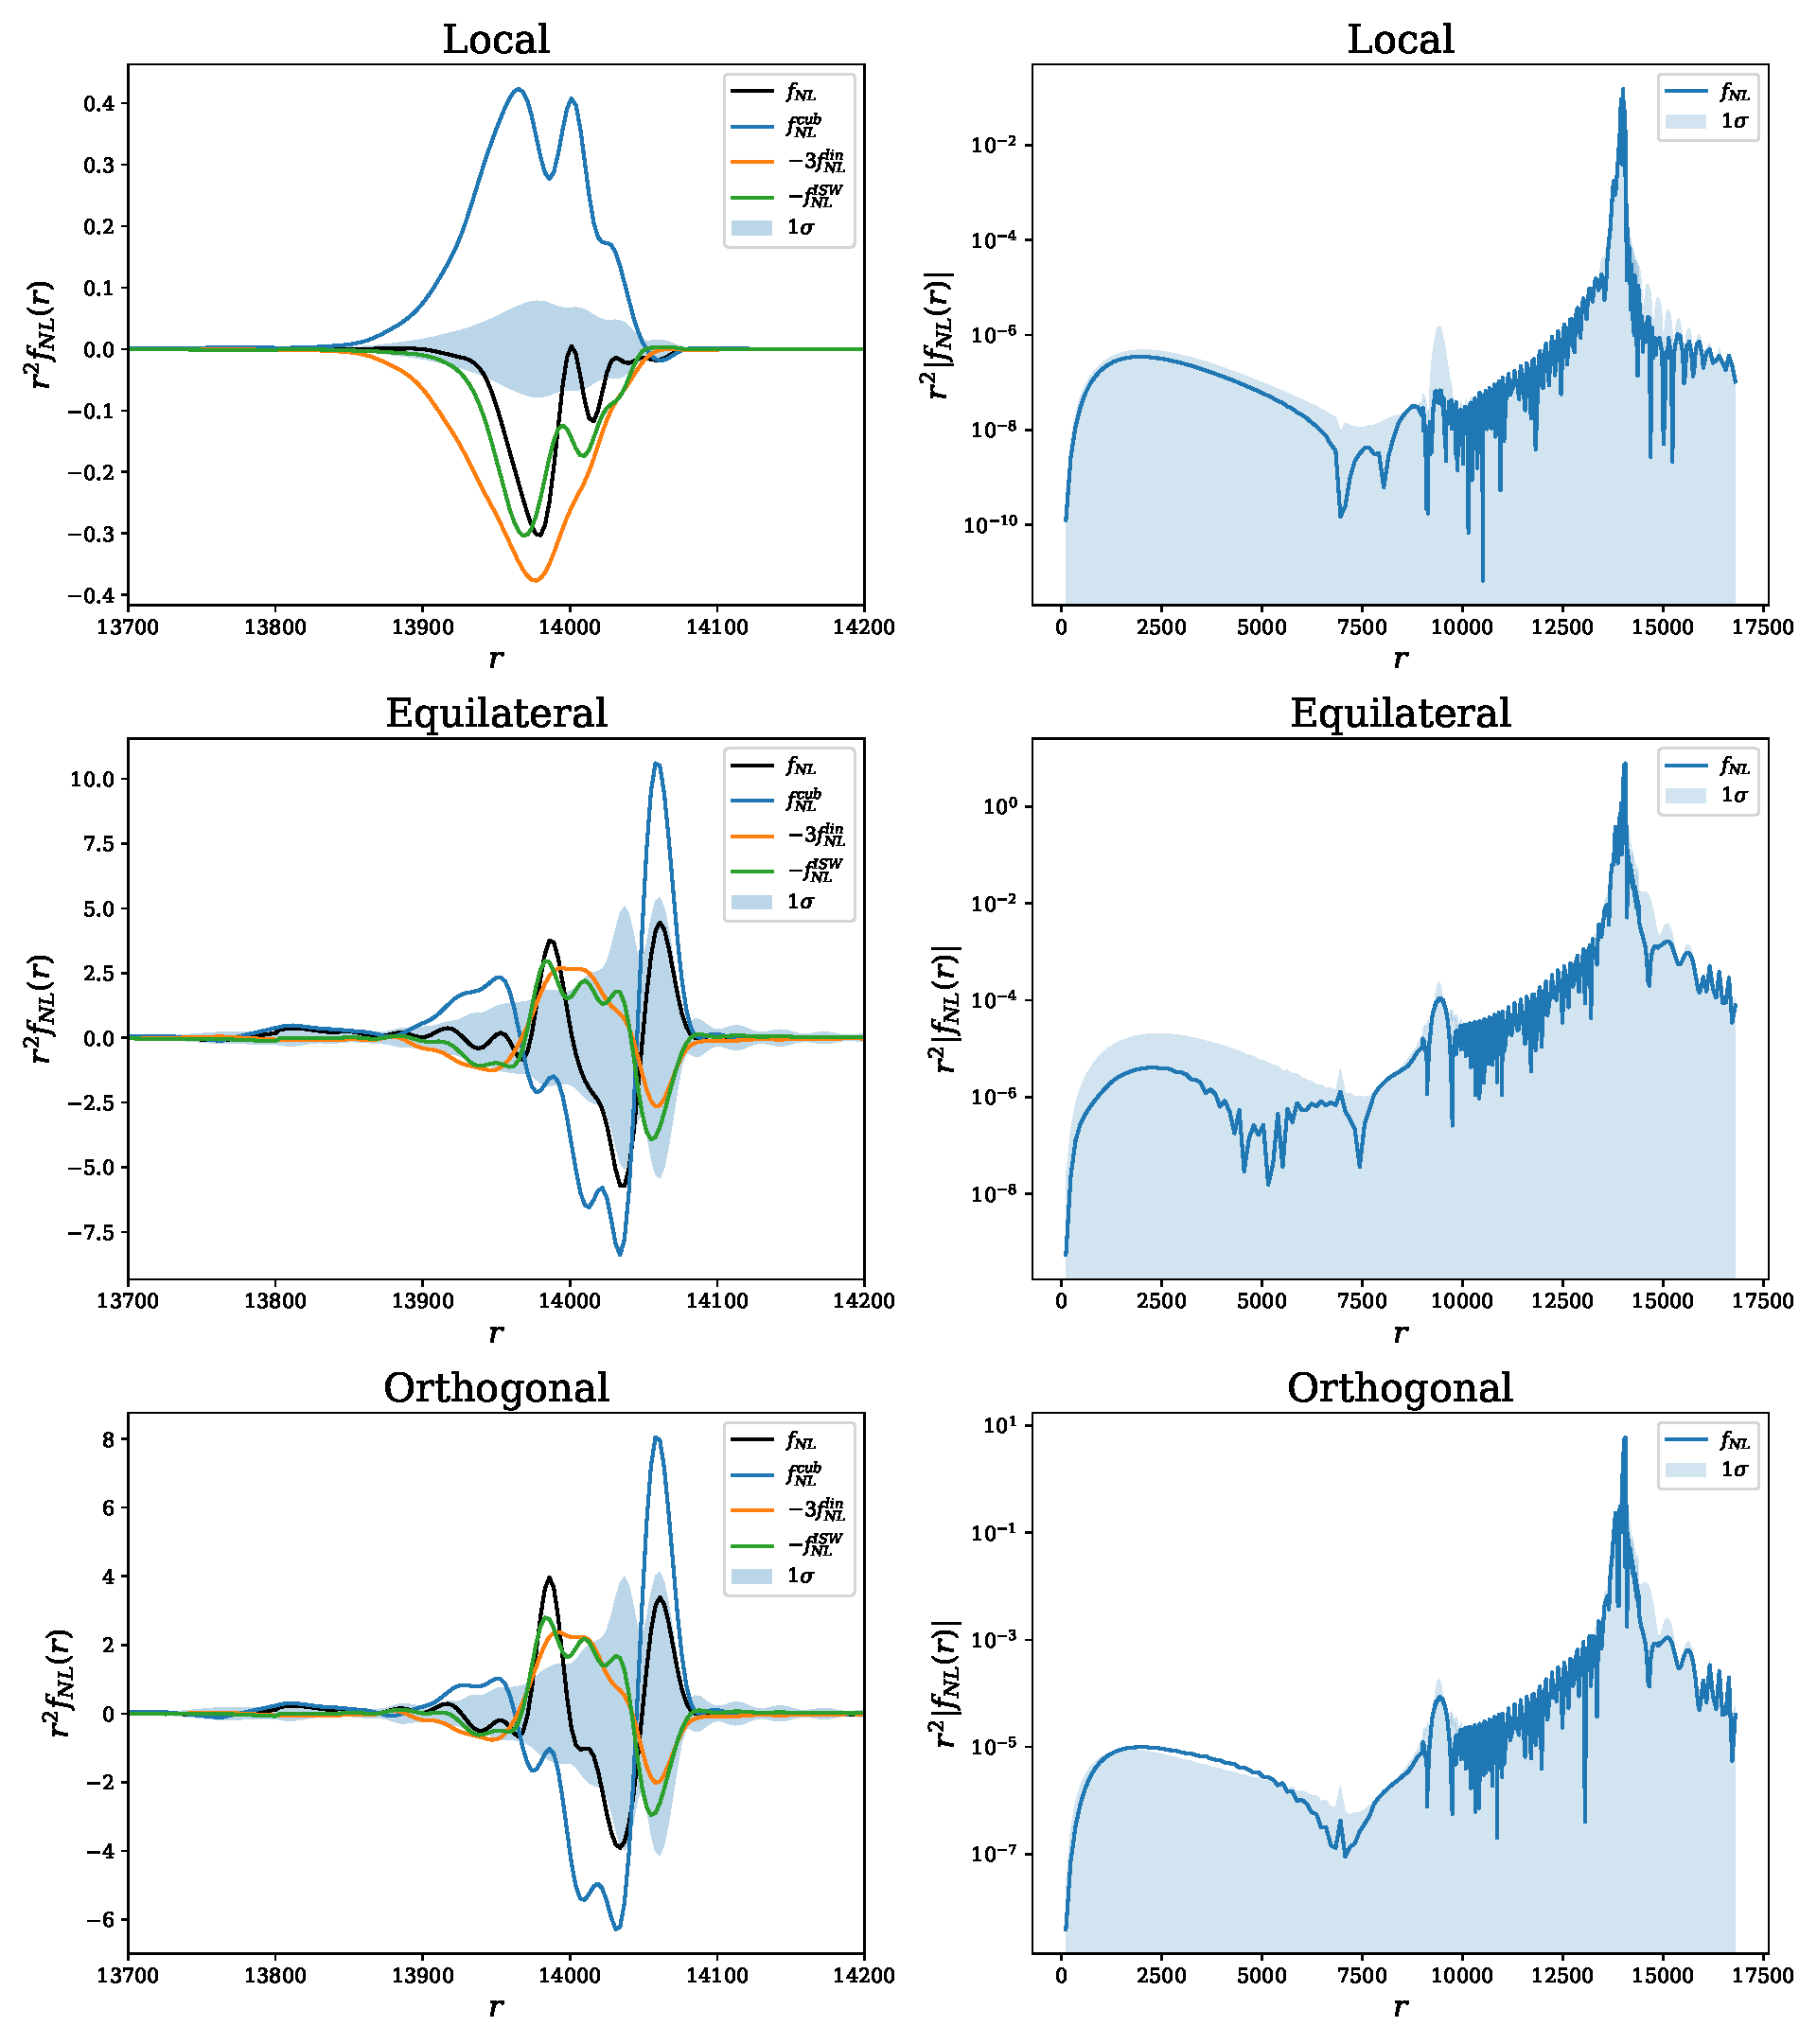
\includegraphics{trio_r_dependence.pdf}
	\caption{Contributions to the total $f_\text{NL}$ from each point in the line-of-sight integral over $r$ for standard templates. On the left-hand side, we plot contributions from the cubic, linear, and lensing-ISW bias, as well as the total $f_\text{NL}$. Shown in blue is the $1\sigma$ interval obtained from the corresponding terms in 140 FFP10 Gaussian simulations. We focus on the $r$ interval around recombination where most of the signal comes from. Plots on the right-hand side show the $f_\text{NL}$ contributions over the whole $r$ range in log scale. The ISW effect, reionisation, and recombination are responsible for the three most noticeable peaks in all three plots.}
	\label{fig:trio_r_dependence}
\end{figure}

As illustrated in plots on the right-hand side of Figure \ref{fig:trio_r_dependence}, the vast majority of signal comes from recombination around $r = 14,000$Mpc. In fact, its contribution is dominant enough that neglecting signals from everywhere else would still be a good approximation. \textsc{CMB-BEst} uses an adaptive $r$ grid which is denser around recombination, following the works of \cite{Smith2011}. Other small but notable contributions to the total estimate come from reionisation ($r \sim 10,000$Mpc) and the ISW effect ($r < 5,000$Mpc).

Zooming in on an interval around recombination, significant contributions from the cubic term to $f_\text{NL}$ of the Local template is rather prominent (upper left of Figure \ref{fig:trio_r_dependence}). The signal is sufficiently larger than the expected random fluctuations evaluated from Gaussian simulations, which could be hinting at non-zero primordial non-Gaussianity. However, contributions from the linear term (shown orange) completely counterbalance it, bringing the total down to values consistent with zero. This again validates the accuracy of our methodology; bias to $f_\text{NL}$ generated from anisotropic sky masks are precisely subtracted off using the linear terms.

We do not find any statistically significant signal across the whole $r$ range otherwise, especially when taking the look-elsewhere effect into account. It is not meaningful to find a couple of 3-4$\sigma$ values when the other 500 points are simply disregarded. If we detect primordial non-Gaussianity in the future, however, then these plots of $f_\text{NL}$ contributions for each $r$ will provide valuable insights into where the signal comes from.




\subsection{Consistency with Planck} \label{section:consistency_with_Planck}

In the previous section, we demonstrated how the integrity of \textsc{CMB-BEst} was validated. The next set of validations involves comparing it against other existing codes for CMB bispectrum estimation.

We test primordial non-Gaussianity constraints on Local, Equilateral and Orthogonal templates against the Planck 2018 analysis \cite{PlanckCollaboration2018}. Two sets of basis functions, KSW and Legendre, have been used to compute $f_\text{NL}$ from the foreground-cleaned CMB map included in the final data release. We choose SMICA as the main component separation method since it was shown to be the most reliable and robust for Planck bispectrum analysis \cite{PlanckCollaboration2013ComponentSeparation, PlanckCollaboration2013,PlanckCollaboration2015,PlanckCollaboration2018}. Table \ref{table:trio_fNL_comparison_with_planck} summarises the constraints obtained, together with the quoted results from the Planck team's own KSW estimator and Modal 2 pipeline.

\begin{table}[h]
	\caption{Constraints on $f_\text{NL}$ for the standard shapes from the KSW and Legendre basis of \textsc{CMB-BEst}, in comparison with the Planck 2018 analysis \cite{PlanckCollaboration2018}. Only the temperature data from the SMICA foreground-cleaned map and FFP10 simulations were used for the analysis. Values shown are after the lensing bias subtraction, with uncertainties at 68\% CL.}
	\centering
	\label{table:trio_fNL_comparison_with_planck}
	\renewcommand{\arraystretch}{1.5} 
	\begin{tabular}{lcccc}
		\toprule
		& \multicolumn{2}{c}{\textsc{CMB-BEst}} & \multicolumn{2}{c}{Planck 2018} \\ \cmidrule(lr){2-3} \cmidrule(lr){4-5}
		Shape & KSW &  Legendre &  KSW &  Modal \\
		\midrule
		
		Local & $-2.2 \;\pm\; 5.5$ & $-2.0 \;\pm\; 5.9$ & $-0.5 \;\pm\; 5.6$ & $-0.6 \;\pm\; 6.4$ \\
		Equilateral & $17 \;\pm\; 61$ & $15 \;\pm\; 62$ & $7 \;\pm\; 66$ & $34 \;\pm\; 67$ \\
		Orthogonal & $-7 \;\pm\; 38$ & $-9 \;\pm\; 38$ & $-15 \;\pm\; 36$ & $-26 \;\pm\; 43$ \\
		\bottomrule
	\end{tabular}
\end{table}

Note that while the constraints from \textsc{CMB-BEst} are largely consistent with Planck 2018 results, there are discrepancies of up to $0.3\sigma$. However, there are variations around this level within the estimates from different pipelines of Planck as well. Equilateral constraints from Planck's own KSW and Modal estimators shown here, for example, differ by $\approx 0.4\sigma$. A similar amount of fluctuation can be found in the full result shown in \cite{PlanckCollaboration2018}. In an ideal world, they should match exactly across different approaches as long as the same dataset is used. However, the statistical significance of the individual $f_\text{NL}$'s is not largely affected by such variations.

We invested a significant proportion of our time investigating this error. Here we discuss three potential areas which might account for the discrepancies. First of all, human error during the implementation and estimation process should not be neglected. Bispectrum analysis is complex and computationally expensive. Implementing it often involves writing a long and heavily optimised code. During the development and testing stages, we found and fixed many mistakes in our $10,000+$ lines of \textsc{C} code. Various unit tests were performed in the process to test individual sections of the code: basis expansion, projection to the $l$ space, SHTs, parallelisation, and more. Internal consistency checks were then used to verify the integrity of the combined pipeline. The Planck team also went to great lengths to validate and cross-check different methods \cite{PlanckCollaboration2013}. It therefore seems unlikely that trivial mistakes are causing the gap in results.

The next source of error we studied is the parameter set. The cosmological parameters we used for constraints in Table \ref{table:trio_fNL_comparison_with_planck} are identical to those of the Planck Modal pipeline. Small changes in cosmological parameters are also shown to have little effect on $f_\text{NL}$ \cite{PlanckCollaboration2015,PlanckCollaboration2018}. One major difference, however, is the number of Gaussian simulations used. We included 140 simulated maps while Modal has about 300. This number is mainly restricted by computational resources required for the large Legendre basis in \textsc{CMB-BEst}. While we found 140 to be sufficient for most cases, sample variance may cause some fluctuation in the linear term and error bar. A rough estimate for sampling error is $\sim \sqrt{2/N_\text{sims}} \approx 0.12$, as calculated in the previous section. Other than $N_\text{sims}$, more internal parameters such as the grid density of discretised arrays have also been checked to yield consistent results when varied. 

We are left with systematic errors as potential causes for discrepancies. The most significant bias to $f_\text{NL}$ constraints is the lensing-ISW bias discussed in Section \ref{section:other_sources_of_non_gaussianity}. Table \ref{table:trio_lensing_bias_comparison_with_planck} shows biases from the lensing bispectrum \cite{Lewis2011lensing} for both \textsc{CMB-BEst} and Planck 2018 analysis. The numbers vary but are consistent overall. Map-by-map comparisons of constraints from the Legendre basis and Modal are shown in Figure \ref{fig:map_by_map_Legendre_Modal}. 

\begin{table}[h]
	\caption{Bias to $f_\text{NL}$ of standard shapes originating from the lensing bispectrum. We compare \textsc{CMB-BEst}'s two different basis sets and the Planck 2018 analysis \cite{PlanckCollaboration2018}, using SMICA map and FFP10 simulations. }
	\centering
	\label{table:trio_lensing_bias_comparison_with_planck}
	\renewcommand{\arraystretch}{1.5} 
	\begin{tabular}{lcccc}
		\toprule
		& \multicolumn{2}{c}{\textsc{CMB-BEst}} & \multicolumn{2}{c}{Planck 2018} \\ \cmidrule(lr){2-3} \cmidrule(lr){4-5}
		Shape & KSW &  Legendre &  KSW &  Modal \\
		\midrule
		
		Local & $7.5$ & $8.2$ & $7.3$ & $6.9$ \\
		Equilateral & $-0.7$ & $-0.6$ & $-0.7$ & $4.0$\\
		Orthogonal & $-22$ & $-22$ & $-23$ & $-25$ \\
		\bottomrule
	\end{tabular}
\end{table}

\begin{figure}[htbp!] 
	\centering    
	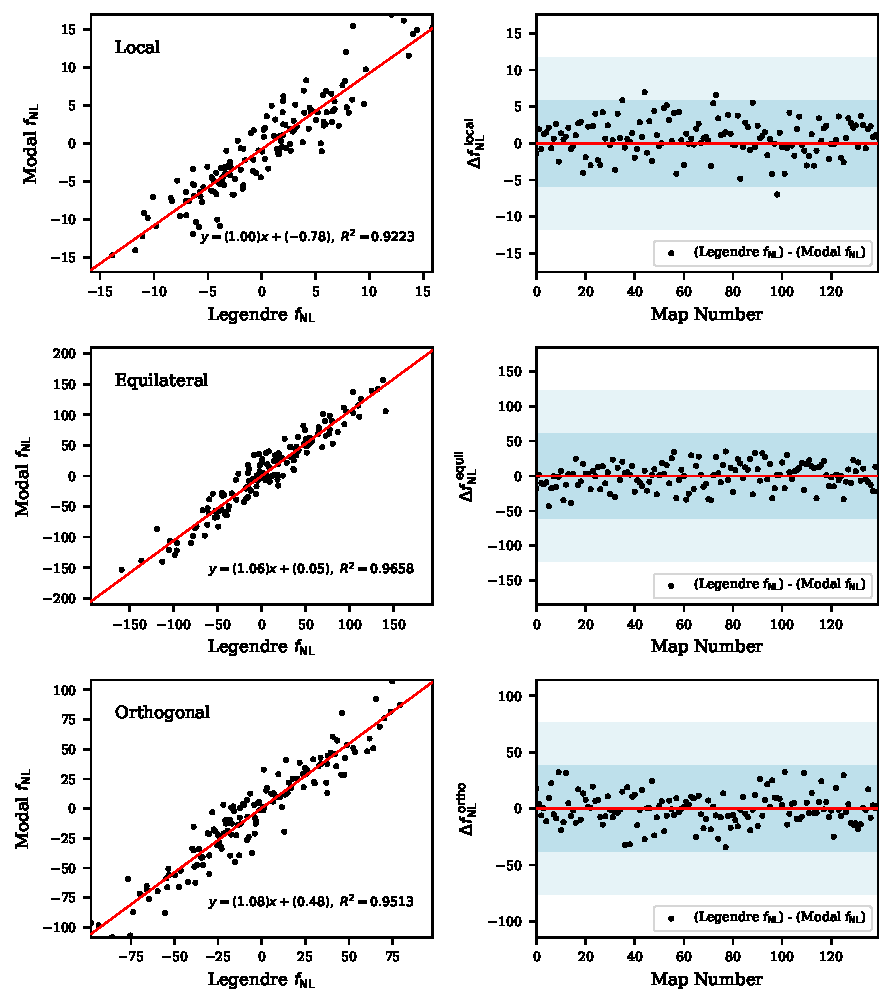
\includegraphics{map_by_map_Legendre_Modal.pdf}
	\caption{A map-by-map comparison of the $f_\text{NL}$ estimates obtained from the \textsc{CMB-BEst}'s Legendre basis set against the Modal estimator results of the Planck 2018 analysis \cite{PlanckCollaboration2018}. The first 140 FFP10 simulations are used here. On the left-hand side are scatter plots where each simulation is represented by a point according to $f_\text{NL}$ estimates of standard templates. Their linear best fit lines are shown in red. Differences in the estimates from the two routines are shown map-by-map on the right-hand side, together with the $1\sigma$ and $2\sigma$ levels shaded in blue. Overall, \textsc{CMB-BEst} and Modal are in good agreement without any significant systematic errors.}
	\label{fig:map_by_map_Legendre_Modal}
\end{figure}

Out of the three templates, the local shape shows the largest scatter between constraints. Comparing $f_\text{NL}$'s of simulated maps from \textsc{CMB-BEst} and Modal, we find a correlation of 0.916. The intercept value of $0.78$ in the linear fit is mainly due to the sample mean present in Modal. Legendre's sample mean is $0.069$ for Local, while Modal's is $-0.698$. Otherwise, the difference between the two pipelines is distributed such that its sample standard deviation equals $2.5$, skewness is $-0.14$, and kurtosis is $0.19$. Having a low level of small skewness and kurtosis of less than $1$ implies that the distribution is close to a univariate normal, consistent with random fluctuation. Similarly, we do not find any significant systematic error from the equilateral and orthogonal shapes either.

Having not found a clear source of error, we conclude that the small gaps between the $f_\text{NL}$ estimates in Table \ref{table:trio_fNL_comparison_with_planck} mainly come from differences in methodology and are consistent with random fluctuations.

We now move on to constraining models with oscillations. The simplest template for oscillatory models is the feature model studied in Chapter \ref{chapter:CMB_state-4_forecast}. We use a template shape function of the form $S^\text{feat}(k_1,k_2,k_3) = \sin(\omega (k_1 + k_2 + k_3) + \phi)$. Figure \ref{fig:sine_template_frequency_Legendre_Modal} shows $f_\text{NL}$ constraints obtained from the Legendre basis and compares them with Modal results from the Planck 2018 analysis. The `phase' $\phi$ is set to zero, while the oscillation `frequency' $\omega$ was varied from $10$ Mpc to $350$ Mpc. We follow \cite{Fergusson2015a} and increase $\omega$ in steps of $10$ so that correlations between shapes with different $\omega$ are kept low.

\begin{figure}[htbp!] 
	\centering    
	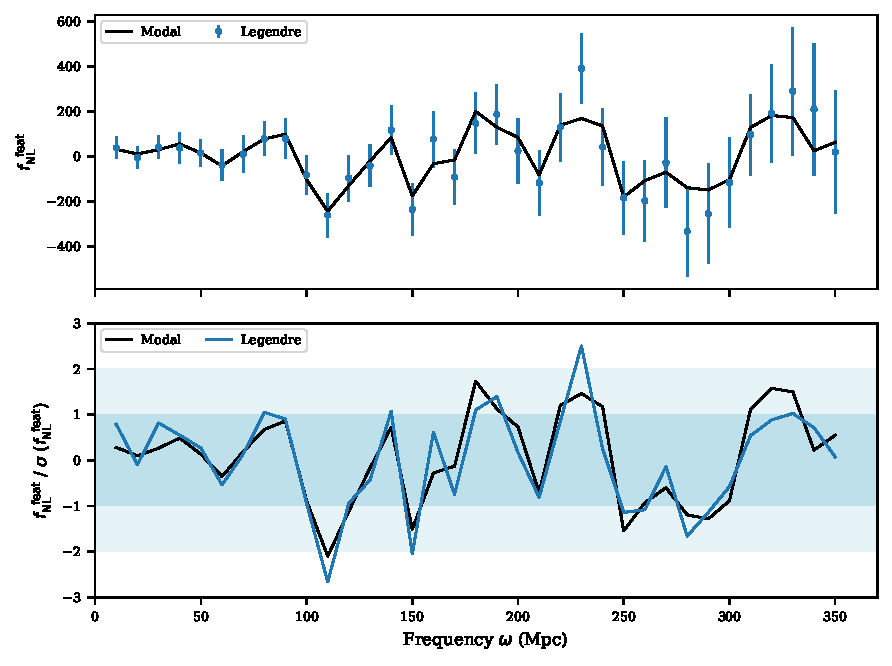
\includegraphics{sine_template_frequency_Legendre_Modal.pdf}
	\caption{The $f_\text{NL}$ estimates for the feature models with $S(k_1,k_2,k_3) = \sin(\omega (k_1 + k_2 + k_3)$, obtained using the Legendre basis (blue) and Planck's Modal (black). Top: a direct comparison of $f_\text{NL}$ for different values of $\omega$. Error bars indicate the expected standard deviations in the estimator calculated using 140 Gaussian simulations. Bottom: signal-to-noise $f_\text{NL}/\sigma\;(f_\text{NL})$, again for a range of $\omega$ values. Shaded in blue are the $1\sigma$ and $2\sigma$ levels. We see that the two approaches yield coherent estimates overall.}
	\label{fig:sine_template_frequency_Legendre_Modal}
\end{figure}

The Legendre basis accurately expands the feature model template using Legendre polynomials via basis expansion outlined in (\ref{eqn:basis_expansion}). Estimates from the two methods, \textsc{CMB-BEst}'s Legendre and Planck's Modal, are mostly compatible. The most notable difference is at $\omega=230$Mpc where $f_\text{NL}$ from Legendre is more than $1\sigma$ larger compared to Modal. Even though it is interesting that the new estimate now passes the $2\sigma$ threshold, having one such point out of 35 shown here has less statistical significance.

Both the Legendre and Modal approaches involve expanding the shape function with respect to a polynomial basis. Polynomials are versatile but have limited resolution for oscillatory signals; it cannot resolve shapes with a number of oscillations greater than the maximum degree of polynomials ($p_\text{max}$ here). For the Legendre basis with $k$ range $[2.09\times 10^{-4}, 2.09\times 10^{-1}]\text{Mpc}^{-1}$ and $p_\text{max}=30$, frequencies greater than $\pi p_\text{max} / (k_\text{max} - k_\text{min}) \approx 436$Mpc are unresolvable. In reality, numerics start to break before this value. We do not have a reference analytic value for true $f_\text{NL}$s, but evaluating correlations between shapes is effective for checking our numerics.

\begin{figure}[htbp!] 
	\centering    
	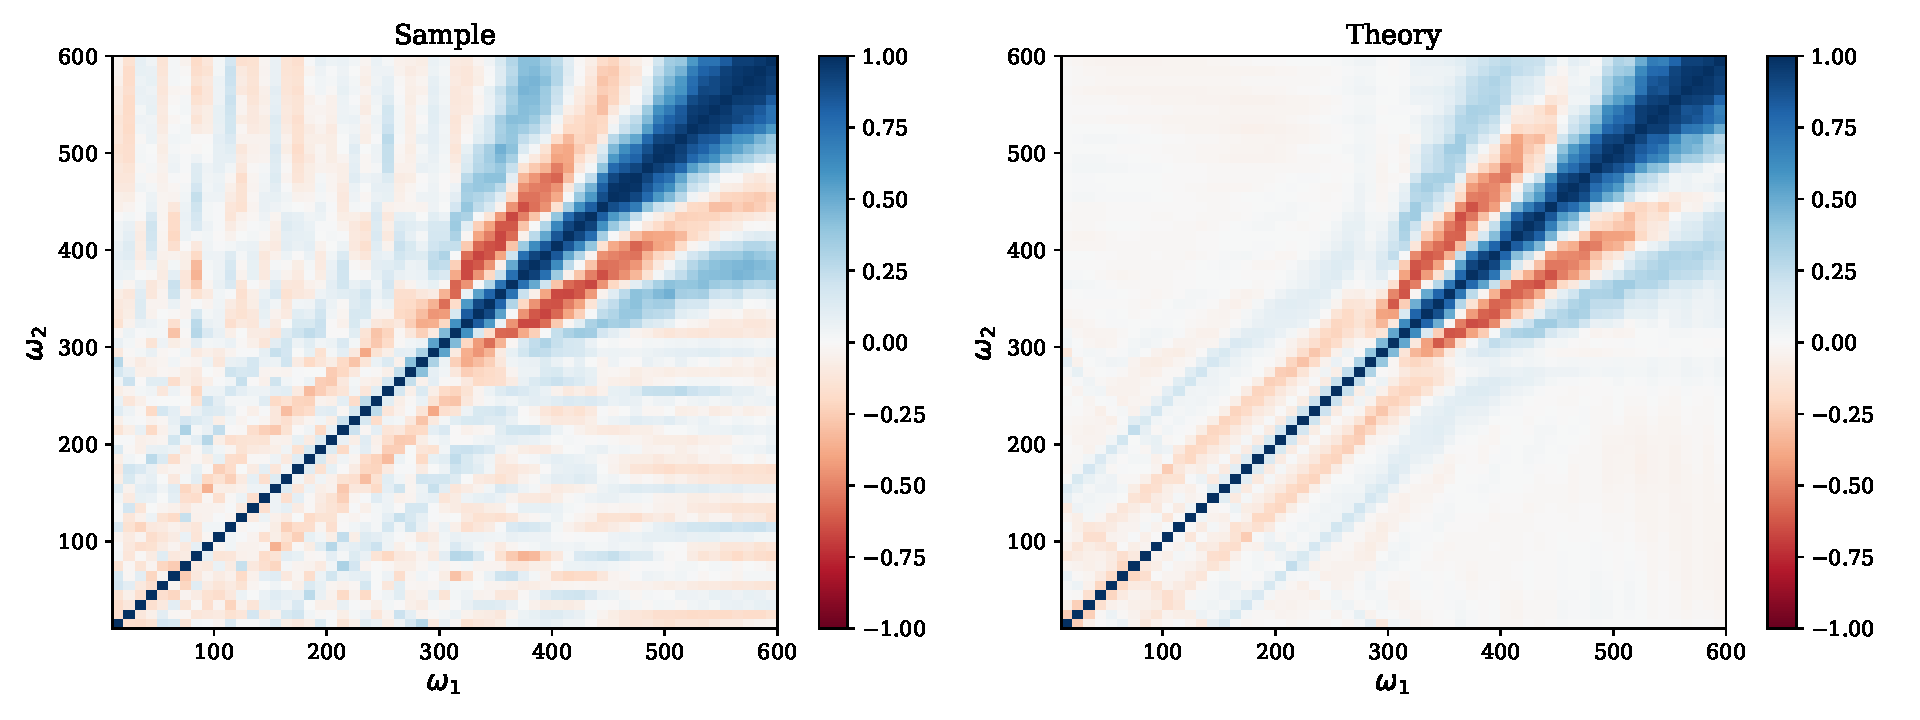
\includegraphics[width=\textwidth]{sine_template_correlations_new.pdf}
	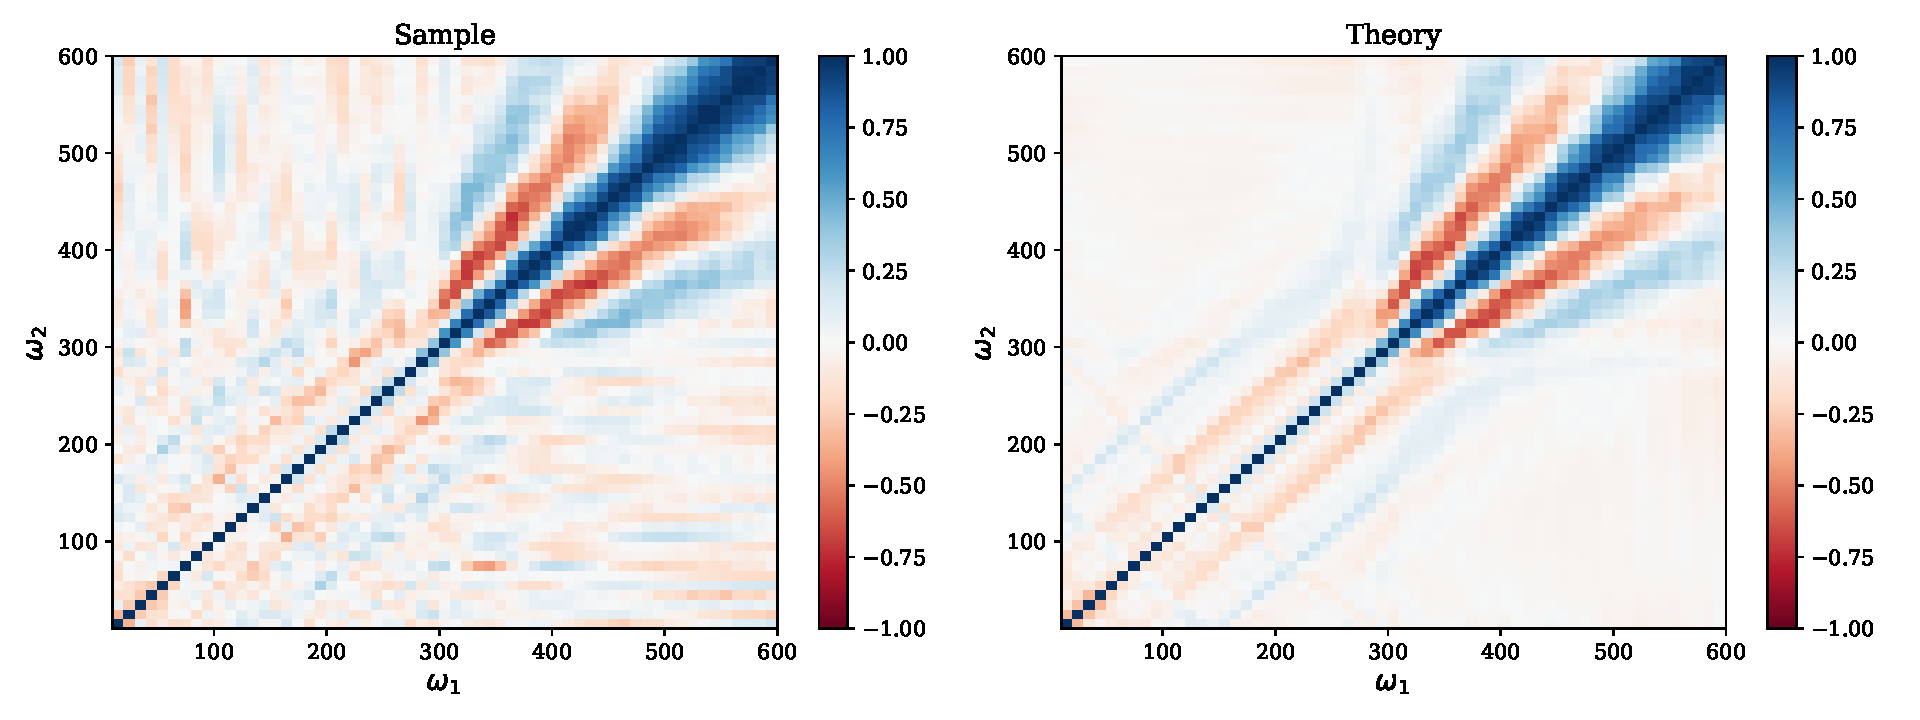
\includegraphics[width=\textwidth]{cosine_template_correlations_new.pdf}
	\caption{Correlations between feature model templates $S(k_1,k_2,k_3)=\sin(\omega (k_1 + k_2 + k_3) + \phi)$ with different $\omega$ values, for $\phi = 0$ (top two) and $\phi = \pi/2$ (bottom two). Results are from the Legendre basis. `Sample' correlations are obtained from $f_\text{NL}$ estimates from 140 Gaussian simulations, while `theory' correlations come from the inner product induced by $\Gamma_{p_1 p_2 p_3, p_1 p_2 p_3}$ matrix in (\ref{def:gamma}). Large non-diagonal correlations appear around $\omega \approx 300$, after which oscillations in the shape are no longer resolved by polynomials of degree up to $p_\textrm{max}$.}
	\label{fig:feature_template_correlations}
\end{figure}

Figure \ref{fig:feature_template_correlations} shows correlations between $f_\text{NL}$s from feature models with different frequency $\omega$s. The plots show the correlation between $f_\text{NL}$ estimates from 140 FFP10 Gaussian simulations (`sample'), together with the one evaluated using our `late-time' inner product ('theoretical') given by
\begin{align}
	\left< b^{(i)}, b^{(j)} \right> &= \sum_{l_j} \frac{h^2_{l_1 l_2 l_3} b^{(i)}_{l_1 l_2 l_3} b^{(j)}_{l_1 l_2 l_3}}{C_{l_1} C_{l_2} C_{l_3}}  \\
	&= \sum_{p_j p'_j} \alpha^{(i)}_{p_1 p_2 p_3} \alpha^{(j)}_{p'_1 p'_2 p'_3} \sum_{l_j} \frac{h^2_{l_1 l_2 l_3} (b^{(i)}_{p_1 p_2 p_3})_{l_1 l_2 l_3} (b^{(j)}_{p'_1 p'_2 p'_3})_{l_1 l_2 l_3}}{C_{l_1} C_{l_2} C_{l_3}} \\
	&= \sum_{p_j p'_j} \alpha^{(i)}_{p_1 p_2 p_3} \alpha^{(j)}_{p'_1 p'_2 p'_3} \Gamma_{p_1 p_2 p_3, p'_1 p'_2 p'_3} \\
	&= \vv{\alpha^{(i)}} \; \Gamma \; \vv{\alpha^{(j)}}, \label{eqn:late_time_inner_product}
\end{align}
where $\Gamma$ is defined in (\ref{def:gamma}). In the limit $N_\text{sims} \rightarrow \infty$, the sample correlation can be shown to approach the theoretical value in the weakly non-Gaussian limit. We see from Figure \ref{fig:feature_template_correlations} that they indeed display the same qualitative behaviour for $N_\text{sims}=140$.

The templates with $\omega < 300$ are highly uncorrelated with each other, as can be seen from small non-diagonal elements. Noticeable correlations on lines $\omega_2 = \omega_1 \pm c$ for $c = 70, 140$ arise from resonance between oscillations and transfer functions at the Baryonic Acoustic Oscillation (BAO) scale, as we observed in Figure \ref{insight feature plot}. Faint lines can also be found near $\omega_2 = -\omega_1 + c, \;\; c = 70,140,210,\cdots$ for similar reasons.

When $\omega > 300$, however, large non-diagonal correlations appear. This is about when the oscillation frequency surpasses the resolution set by the highest degree of polynomials. Our basis expansion becomes inaccurate after this point. There are interesting linear structures present, with slopes roughly equal to $2, 1/2$ and subsequently $4, 1/4$. These lines come from aliasing caused by subsampling rapid oscillations; our basis picks up $\omega' = \omega/2$ signal instead. $\omega_2/2 = -\omega_1 + 70$ and other pairs of $(\omega_1, \omega_2)$ resonate to give large non-diagonal correlations.

We verify our claim that numerical inaccuracies at high $\omega$s are caused by the lack of resolution due to a limited number of polynomial modes. Figure \ref{fig:feature_template_correlations_compare_lmax} illustrates how having a smaller $k$ range allows us to constrain faster oscillations more accurately. Note that we also change $l_\text{max}$ correspondingly since smaller scales are neglected. The plot on the right-hand side uses a Legendre basis with the $(k_\text{min}, k_\text{max})$ range rescaled by a factor of $3/4$. Fewer oscillations appear within the $k$ interval and are therefore easier to expand using fewer polynomials. As we expected, the scale at which non-diagonal correlations blow up is now shifted to a higher frequency, $\omega \approx (4/3) \cdot 300$. 

\begin{figure}[htbp!] 
	\centering    
	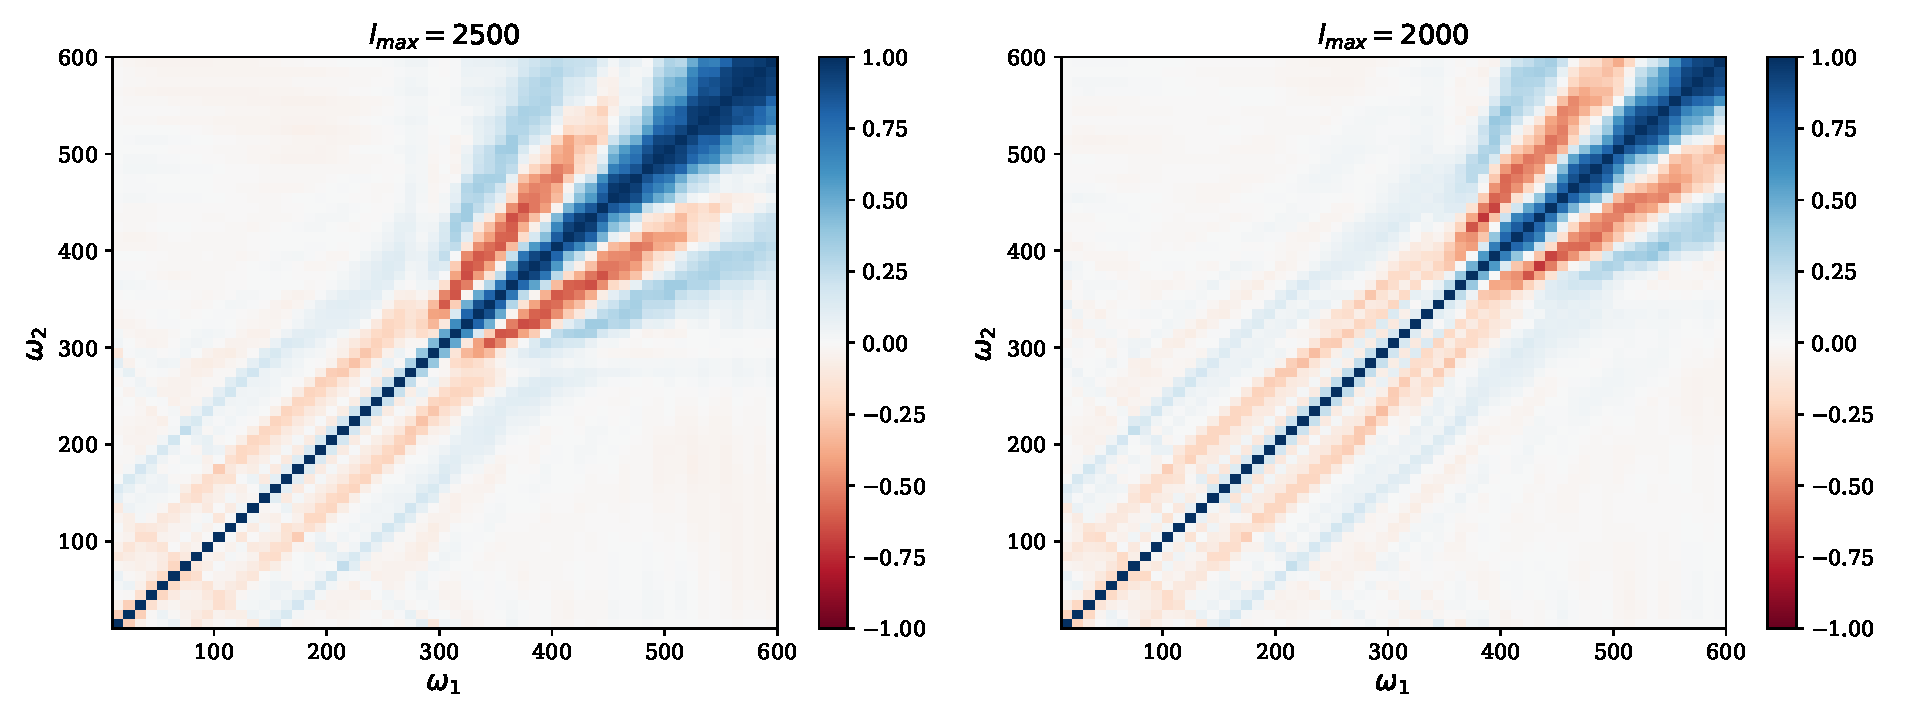
\includegraphics[width=\textwidth]{sine_template_correlations_compare_lmax_new.pdf}
	\caption{Theoretical correlations between feature model templates with different frequency $\omega$s, as described in Figure \ref{fig:feature_template_correlations}. The phase $\phi$ is set to zero in both cases, while the right plot is obtained from the Legendre basis with a different $k$ range. The maximum $l$ value is reduced from $2500$ to $2000$, shifting $(k_\text{min},k_\text{max})$ by a factor of $2000/2500 = 0.75$. Having a smaller $k$ range means fewer oscillations within the $k$ interval for same $\omega$ which provides better effective resolution. The right plot does indeed show smaller non-diagonal correlations at high frequencies.}
	\label{fig:feature_template_correlations_compare_lmax}
\end{figure}

There is a subtlety around the $f_\text{NL}$ estimates obtained from inaccurate primordial basis expansions. \textsc{CMB-BEst} computes $\beta$s and $\Gamma$s with respect to a fixed Legendre basis, which has been shown to be accurate for each and every polynomial mode. Therefore, even when the primordial basis is unable to resolve rapid oscillations, the $f_\text{NL}$ estimates we obtain are nevertheless meaningful; they are simply probing a different model. The constraints are not for the given shape function, but rather its projection to the vector subspace spanned by the basis functions as shown in (\ref{eqn:primordial_basis_projection}). Detecting a non-zero $f_\text{NL}$ here can still have significant implications.

Another popular template for models with oscillations is the `resonance' shape parametrised as $S(k_1, k_2, k_3) = \sin(\omega \log(k_1 + k_2 + k_3 ) + \phi)$. Log-spaced oscillations are numerically harder to deal with since the oscillation frequency diverges as $k \rightarrow 0$. Note also that any scaling factors to the $k$'s can be absorbed into the phase via $\log(c(k_1 + k_2 + k_3)) = \log(k_1 + k_2 + k_3) + \log(c)$. For our Legendre basis with $k_\text{max}/k_\text{min}$ fixed to $1000$, the full $k$ range includes $\approx 1.1\omega$ oscillations. Any frequency larger than $\approx 27$ therefore cannot be expanded using $p_\text{max}=30$ polynomials. We still explore shapes with higher $\omega$s, however, since the basis can pick up slower oscillations in higher $k$ values. Corresponding constraints should be taken with a grain of salt; they probe bispectrum shapes \textit{similar} to the resonance template. Low-$k$ oscillations are especially likely to be wiped out from these shapes.

Figure \ref{fig:sinlog_template_frequency_Legendre_Modal} compares $f_\text{NL}$ constraints for the resonance template over a range of $\omega$s. As can be seen from the top two plots, the signal-to-noise values obtained from the Legendre basis and Modal are relatively consistent up until $\omega \approx 35$, after which the two results start diverging significantly. The threshold is about the same for `sinlog' ($\phi = 0$) and `coslog' ($\phi=\pi/2$) shapes.

Recall that the sample $\sigma$ from $f_\text{NL}$ estimates of Gaussian simulations should converge to the theoretical value calculated from the Fisher information as $N_\text{sims}\rightarrow\infty$, since the CMB bispectrum estimator is optimal. We have checked that the sample and theoretical variances are consistent for standard templates in Section \ref{section:internal_consistency}, using both KSW and Legendre basis sets. The bottom two plots in Figure \ref{fig:sine_template_frequency_Legendre_Modal} show the equivalent results for the resonance template with varying $\omega$.

\begin{figure}[htbp!] 
	\centering    
	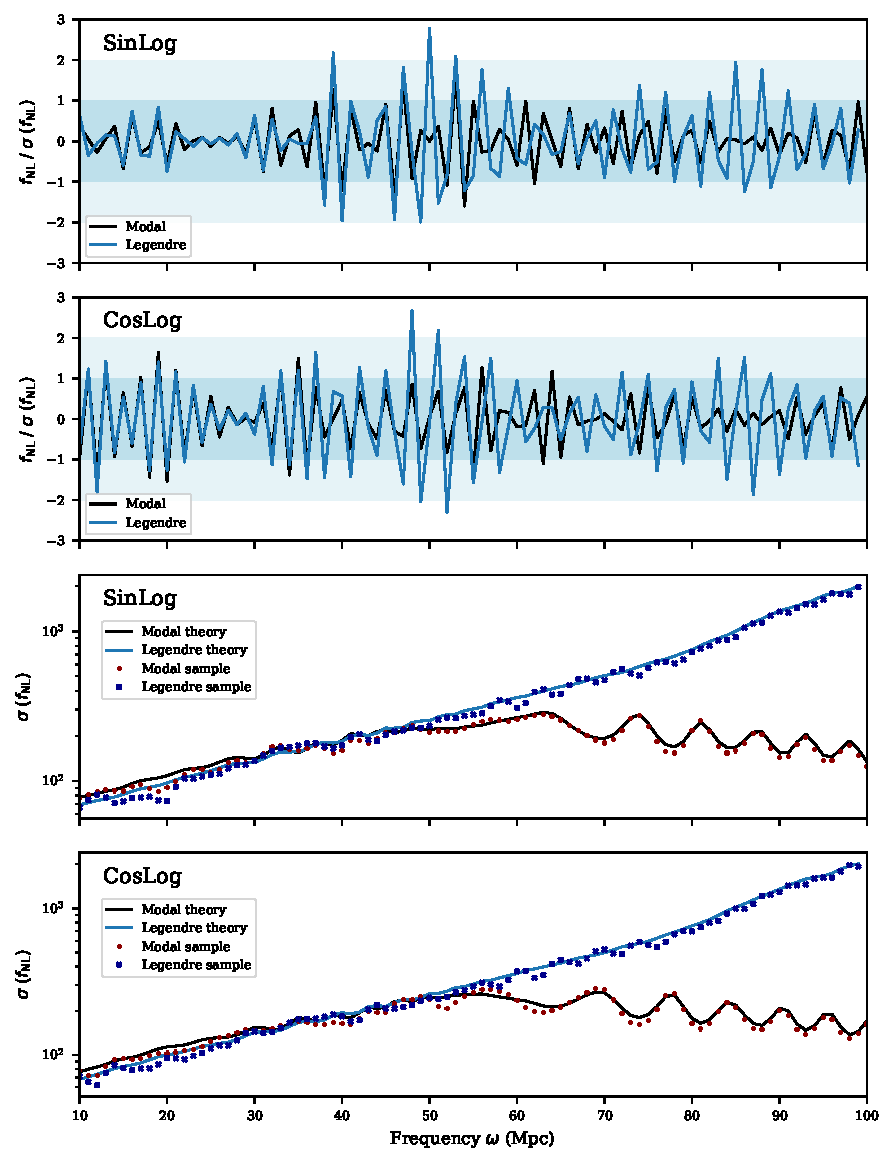
\includegraphics{sinlog_template_frequency_Legendre_Modal.pdf}
	\caption{Constraints for the resonance shape $S(k_1,k_2,k_3) = \sin(\omega \log(k_1 + k_2 + k_3 ) + \phi)$ with varying frequency $\omega$s, while the phase $\phi$ is set to $0$ (`SinLog') and $\pi/2$ (`CosLog'). Results are obtained using \textsc{CMB-BEst}'s Legendre basis (blue) and Planck's Modal estimator (black). Top two: signal-to-noise significance of the estimated $f_\text{NL}$s with their $1\sigma$ and $2\sigma$ levels shaded in blue. Bottom two: standard deviations of the $f_\text{NL}$ estimates against $\omega$ calculated from $f_\text{NL}$s of 140 Gaussian simulations (sample) and the $\Gamma$ matrix (theory).}
	\label{fig:sinlog_template_frequency_Legendre_Modal}
\end{figure}

Similarly to the feature models studied in Chapter \ref{chapter:CMB_state-4_forecast}, uncertainty in the estimated $f_\text{NL}$s increases as we raise $\omega$, exploring more rapid oscillations in the bispectrum. Both the Modal and Legendre methods lose their ability to resolve shapes with $\omega$s larger than $35$. The constraints are then no longer for the precise resonance shape but rather an approximation to it. A notable difference between Modal and \textsc{CMB-BEst}'s Legendre basis is their behaviour at high $\omega$. Modal's numerical accuracy is completely lost after $\omega\approx 50$, leading to disproportionately large bispectra and small $\sigma$. On the other hand, Legendre retains stability in its basis expansion, yielding constraints for approximate bispectrum shapes closest to the true, high-frequency ones.

\begin{figure}[htbp!] 
	\centering    
	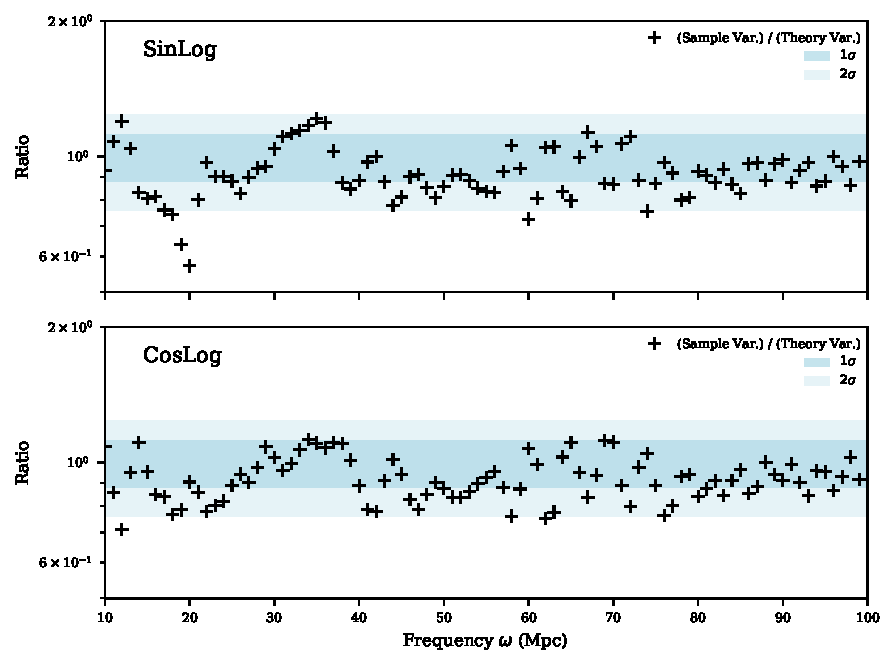
\includegraphics{sinlog_template_frequency_variances_Legendre.pdf}
	\caption{Ratios between the sample and theoretical variances obtained from the Legendre basis for resonance shapes. The sample variance is calculated from the $f_\text{NL}$ estimates of $140$ Gaussian simulations. The $1\sigma$ and $2\sigma$ intervals (shaded in blue) are chosen based on a $\chi^2$-distribution, which accurately describes the statistics of the sample variance as long as the $f_\text{NL}$s are Gaussian distributed. The results are statistically consistent with random fluctuations except potentially at $\omega=20$, as discussed in the main text.}
	\label{fig:sinlog_template_frequency_variances_Legendre}
\end{figure}

A detailed comparison between the sample and theoretical variances is depicted in Figure \ref{fig:sinlog_template_frequency_variances_Legendre}. This serves as a useful consistency check within the \textsc{CMB-BEst} pipeline. Sample variances are calculated from a finite number of $f_\text{NL}$ samples from simulations. We test if these estimates are compatible with the underlying distribution: $\chi^2$ with $N_\text{sims}-1$ degrees of freedom in this case. We achieve the desired consistency for both $\phi=0$ and $\phi=\pi/2$. One potentially meaningful outlier is at $\omega=20$ and $\phi=0$, where the sample estimate is below 60\% of the expected level. This anomaly is not likely to be a numerical error specific to \textsc{CMB-BEst} since a similar dip can be found from Modal results in Figure \ref{fig:sinlog_template_frequency_Legendre_Modal}. No significant irregularity is found for different phases at the same frequency. We classify this point as a random fluctuation for now, but a further investigation using an independent set of Gaussian simulations is required to be certain.

As with the feature models before, we plot the correlation matrix between the templates with different $\omega$s in Figure \ref{fig:sinlog_template_correlations}. Shapes with similar $\omega$s are naturally correlated, but most off-diagonal terms of the matrix vanish. Even for $\omega > 35$ where the basis expansion becomes less accurate, cross-correlations tend to remain small until $\omega \approx 75$. We verify the stability of \textsc{CMB-BEst}'s Legendre basis expansion; best approximations to the highly oscillatory template are found, allowing us to continue exploring independent bispectrum shapes with the characteristic log-spaced oscillations.

\begin{figure}[htbp!] 
	\centering
	(a) $ \phi=0 $
	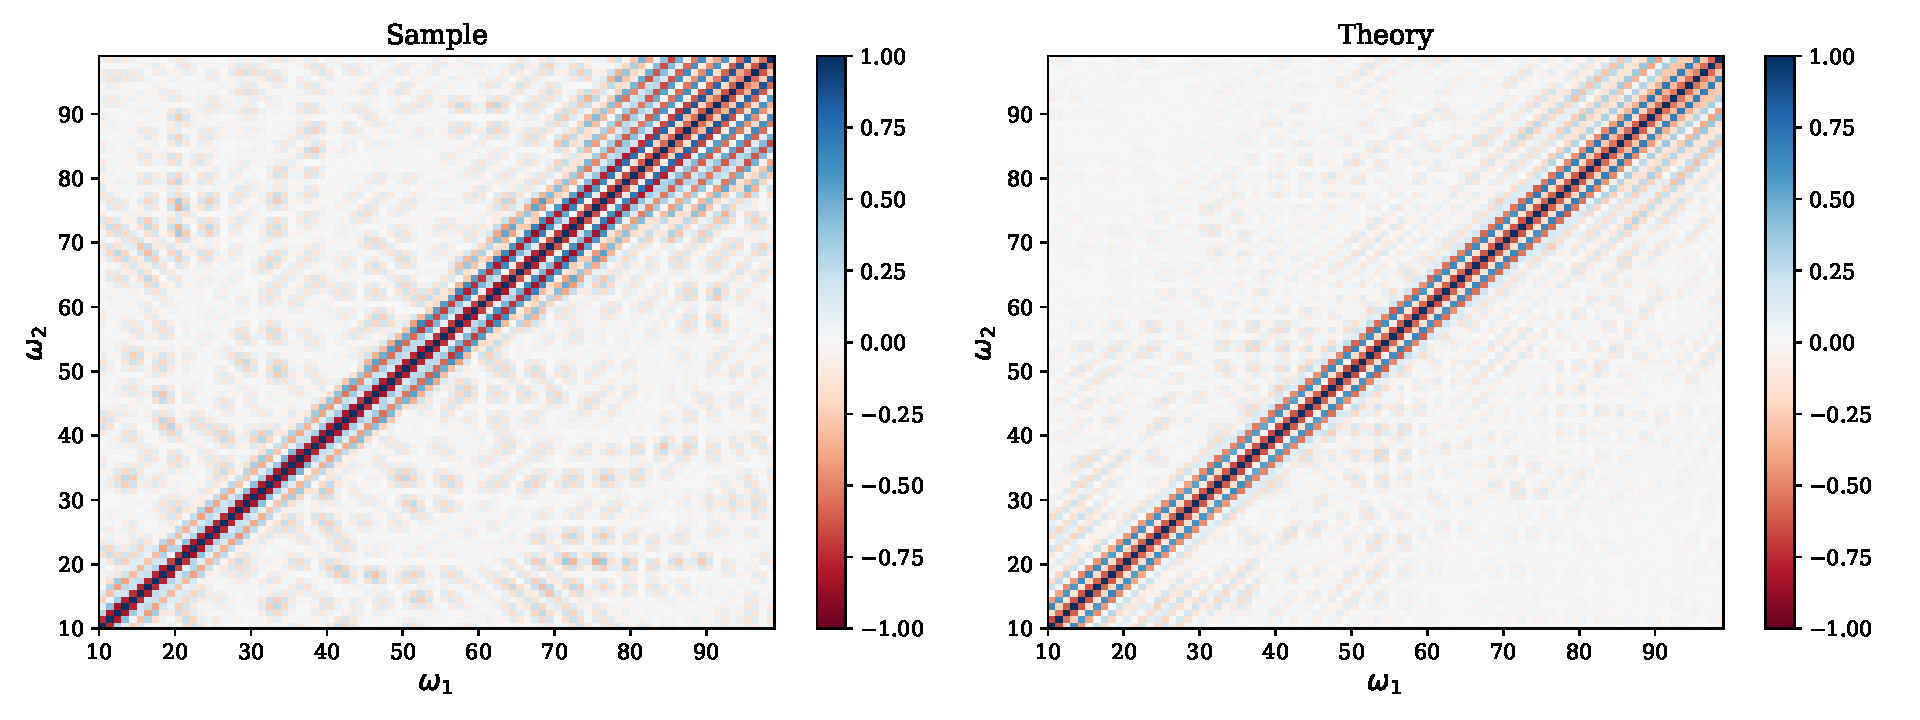
\includegraphics[width=\textwidth]{sinlog_template_correlations_new.pdf}
	(b) $ \phi=\pi/2 $
	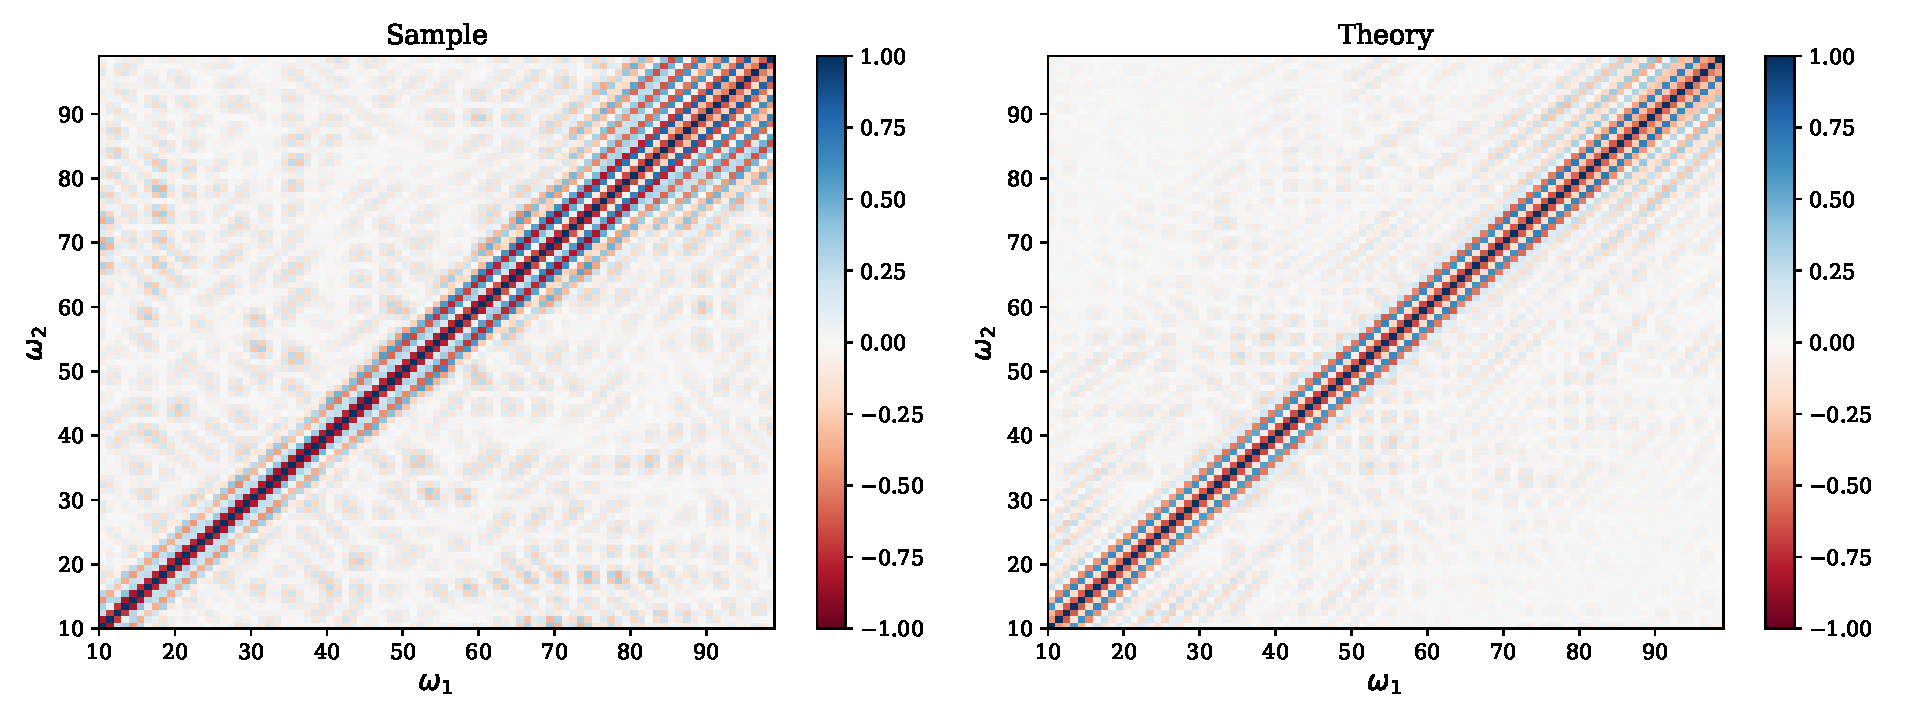
\includegraphics[width=\textwidth]{coslog_template_correlations_new.pdf}
	\caption{Correlations between the resonance model templates of shape given by ${S(k_1,k_2,k_3) = \sin(\omega\log(k_1+k_2+k_3)+\phi)}$ with different $\omega$ values, for (a) $\phi = 0$ and (b) $\phi=\pi/2$. `Sample' correlations are obtained from the Legendre basis $f_\text{NL}$ estimates from 140 Gaussian simulations. `Theory' correlations come from the inner product induced by $\Gamma$ as shown in (\ref{eqn:late_time_inner_product}).}
	\label{fig:sinlog_template_correlations}
\end{figure}


\subsection{Proof of concept} \label{section:proof_of_concept}


\textsc{Primodal} is a fast and efficient numerical code for computing bispectra of primordial perturbations given a single field inflation Lagrangian using in-in formalism \cite{Clarke2021}. The computed bispectrum is expressed as coefficients of a separable basis expansion in \textsc{Primodal}, as opposed to a grid of discrete points like other in-in codes. Choosing an equivalent basis set for \textsc{CMB-BEst} therefore creates a direct link between the two codes. The combined pipeline is capable of constraining specific inflation models directly without the use of approximate templates. Such template-free bispectrum analysis also enables a fast and extensive scan of theory parameters.

Collaborating closely with the main author of \textsc{Primodal}, Philip Clarke, we verified the integrity of the combined \textsc{Primodal} + \textsc{CMB-BEst} routine. We thoroughly tested the consistency of basis functions, their orthogonalisation, and convergence. Both \textsc{Primodal} and \textsc{CMB-BEst} are now in the exploitation phase. We present a working example of the combined pipeline as a proof of concept.

DBI inflation \cite{Silverstein2004dbi,Alishahiha2004dbi,Chen2005runningdbi,Bean2008comparingdbi} is a well-studied single-field inflation model inspired by string theory. Its action follows the general form \eqref{eqn:general_single_field_action}, with a non-canonical kinetic term given by
\begin{align}
	P(X,\phi) = - \frac{1}{f(\phi)} \left[ \sqrt{1 - 2f(\phi)X} - 1 \right] - V(\phi),
\end{align}
where $X=-\frac{1}{2} g^{\mu\nu} \partial_\mu \phi \partial_\nu \phi$ as before. $f(\phi)$ is an arbitrary function called the warp factor. We choose
\begin{align}
	f(\phi) = \frac{\lambda_\text{DBI}}{\phi^4}, \qquad V(\phi) = V_0 - \frac{1}{2}m^2\phi^2, \qquad m = \sqrt{\beta_\text{IR}} \; H,
\end{align}
for some theory parameters $\lambda_\text{DBI}$, $V_0$, and $\beta_\text{IR}$. The sound speed can then be obtained from \eqref{eqn:general_single_field_sound_speed}, which evaluates to $c^\text{DBI}_\text{s} \approx 3/\beta_\text{IR} N_e$ under some slow-roll approximations \cite{Chen2005runningdbi}. Here, $N_e$ denotes the number of e-folds until the end of inflation.

DBI inflation generates non-Gaussianity with its shape similar to the equilateral template \eqref{def:equilateral_template}. The latest constraints on the model come from the Planck CMB bispectrum analysis using an approximate template 
\begin{align}
	B_\Phi^\text{DBI}(k_1,k_2,k_3) = \frac{6A_\Phi^2}{(k_1 k_2 k_3)^3} \frac{-3/7}{(k_1 + k_2 + k_3)^2} \bigg[ \sum_i k_i^5 &+ \sum_{i\neq j} (2k_i^4 k_j - 3k_i^3 k_j^2)  \nonumber \\
	&+ \sum_{i\neq j\neq l} (k_i^3 k_j k_l - 4k_i^2 k_j^2 k_l) \bigg]. \label{eqn:dbi_bispectrum_template}
\end{align}
We switched to a convention where the potential $\Phi$ is used instead of $\zeta$. On superhorizon scales at the end of inflation, they differ by a constant factor: $\Phi = (3/5)\zeta$. With respect to this template, the theoretical bispectrum from DBI inflation has an amplitude equal to
\begin{align}
	f_\text{NL}^\text{DBI} \approx - \frac{35}{108} \left[ \frac{1}{\left( c^\text{DBI}_\text{s} \right)^2} - 1 \right], \label{eqn:DBI_fNL_and_sound_speed}
\end{align}
an approximation which is accurate as long as the DBI sound speed $c^\text{DBI}_\text{s} \ll 1$. Constraints on $f_\text{NL}^\text{DBI}$ therefore place limits on $c_\text{s}$. Planck 2018 analysis \cite{PlanckCollaboration2018} found $f_\text{NL}^\text{DBI} = 46 \;\pm\; 58$ with a 68\% confidence level from CMB temperature data. The corresponding bound on the speed of sound is $c^\text{DBI}_\text{s} \ge 0.079$.

We reproduce the DBI sound speed constraint from Planck 2018 analysis using the \textsc{Primodal}$+$\textsc{CMB-BEst} routine. Unlike the Planck analysis, our method does not require templates to connect inflationary predictions to CMB data. Instead of using a single estimate from an approximate template, we scan over DBI theory parameters and constrain the individual primordial bispectrum directly. A given parameter set can be ruled out if the corresponding constraint on $f_\text{NL}$ excludes $f_\text{NL}=1$ with high confidence. 

One notable limitation in the current implementation of \textsc{Primodal} is that the details of how inflation ends are not prescribed. This means that the scales during inflation and what we observe cannot be mapped directly, which restricts our ability to translate the results into a constraint on more fundamental parameters such as $\beta_\text{IR}$. Our work here still serves as a useful validation of the combined pipeline. For the DBI sound speed scan, the approximate relation \eqref{eqn:DBI_fNL_and_sound_speed} is used to relate the output $c^*_s$\textemdash sound speed at some pivot scale during horizon crossing\textemdash from \textsc{Primodal} with the physical DBI sound speed $c^\text{DBI}_\text{s}$. Numerous other validation tests we performed such as convergence tests with respect to the basis size $p_\text{max}$ are unaffected by this caveat and still serve as a proof of concept for our combined pipeline.

The parameter $\beta_\text{IR}$ is varied within the interval $[0.1885,0.58]$ while fixing other parameters as $\lambda_\text{DBI} = 2.00475 \times 10^15$, $V_0 = 5.2 \times 10^{-12} M^4_\text{pl}$, and $\phi_0 = 0.46042 M_\text{pl}$, where $M_\text{pl}$ is the Planck mass. Further details of the scan will be included in \cite{Sohn2021inprep}. The results are depicted in Figure \ref{fig:dbi_sound_speed_scan}.

\begin{figure}[htbp!] 
	\centering    
	\includegraphics{dbi_sound_speed_scan_annotated.pdf}
	\caption{Constraints on the DBI model with varying sound speed $c_\text{s}$. Primordial bispectrum computed from \textsc{Primodal} is fed directly into \textsc{CMB-BEst} in the form of coefficients $\alpha_{p_1 p_2 p_3}$ appearing in Legendre basis expansion. Constraints from the Legendre basis with $p_\text{max}=30$ (black $+$) are shown in comparison with $p_\text{max}=29$ (black $\times$). $1\sigma$ and $2\sigma$ confidence intervals around $0$ are shaded in blue and represent the uncertainty in the estimated $f_\text{NL}$s. Bispectrum shapes are normalised so that $f_\text{NL}=1$ corresponds to the DBI model under consideration. Our constraint on DBI sound speed is $c^\text{DBI}_\text{s} > 0.056$ with $95\%$ confidence level. Equivalent results from an approximate DBI bispectrum template \eqref{eqn:dbi_bispectrum_template} (blue dashed) give the $c^\text{DBI}_\text{s}$ bound which is identical up to two significant figures.}
	\label{fig:dbi_sound_speed_scan}
\end{figure}

First of all, we check that our Legendre basis with $p_\text{max}=30$ has converged and accurately represents the primordial bispectrum from DBI inflation. Values of the $f_\text{NL}$ estimates obtained from $p_\text{max}=30$ were tested against the equivalent result with $p_\text{max}=29$ and shown to differ by less than $0.01\%$, as can be seen in Figure \ref{fig:dbi_sound_speed_scan}. In order to thoroughly investigate the degree of convergence, we studied a late-time equivalent of $\epsilon$ in  \eqref{def:primordial_shape_epsilon} used to compare primordial bispectrum shapes;
\begin{align}
	\epsilon^2 (\vv{f}_1, \vv{f}_2) = \frac{1}{N_\text{sim}}  \sum_{i=1}^{N_\text{sim}} \left( \frac{f^{(i)}_1}{\sigma_1} - \frac{f^{(i)}_2}{\sigma_2} \right)^2,
\end{align}
where $f^{(i)}_1$ and $f^{(i)}_2$ denote the $f_\text{NL}$ estimates for the $i$th Gaussian simulated map from the two routines. $\epsilon^2$ measures the mean squared error in the two sets of $f_\text{NL}$ signal-to-noises for $N_\text{sim}$ simulations. Comparing results from the Legendre basis with $p_\text{max} = 30$ and $25$ across the scan, we confirmed that $\epsilon < 0.01$ in the full range and $\epsilon \approx 0.002$ for the majority. A plot with the full result will be provided in \cite{Sohn2021inprep}.

Secondly, we constrain the DBI sound speed as $c_\text{s} \gtrapprox 0.056$ with $95\%$ confidence using CMB temperature data from Planck. Each of the points in Figure \ref{fig:dbi_sound_speed_scan} is normalised to some $\tilde{f}_\text{NL}$ such that $\tilde{f}_\text{NL}=1$ corresponds to the bispectrum predicted by the model. Estimates from the Planck 2018 map take negative values with error bars small enough to exclude $f_\text{NL}=1$ with $2\sigma$ confidence level when $c_\text{s} < 0.056$. Our constraint is similar but not identical to the result from Planck 2018 analysis which reads $c_\text{s} \ge 0.079$. The discrepancy stems from differences in the constraints for the DBI template \eqref{eqn:dbi_bispectrum_template}: $f^\text{DBI}_\text{NL}=27 \pm 58$ for \textsc{Primodal}+\textsc{CMB-BEst} whereas $f^\text{DBI}_\text{NL}=46 \pm 58$ for Planck. This $\approx0.32\sigma$ gap in signal to noise is mainly because the Modal expansion is incomplete and the correlation between the expanded and full DBI template equals $r\approx 0.95$. As discussed in Appendix B of \cite{PlanckCollaboration2013}, this level of correlation causes an expected scatter in $f_\text{NL}$s approximately equal to $0.3\sigma$.

Lastly, we verify that the DBI template \eqref{eqn:dbi_bispectrum_template} accurately approximates the full numerical result obtained from \textsc{Primodal}. Drawn in blue-dashed on Figure \ref{fig:dbi_sound_speed_scan}, the difference between the $\tilde{f}_\text{NL}$ constraints obtained using \textsc{Primodal} and the DBI template differ by $O(0.01\sigma)$.

\bigskip

We extend the \textsc{Primodal}+\textsc{CMB-BEst} pipeline to study DBI models with resonance. The primordial bispectrum appears similar to the DBI template but has extra log-spaced oscillations superimposed. The Planck analysis covered the DBI shape and the resonance templates independently \cite{PlanckCollaboration2018} but has not constrained the combination of the two. Our method studies the bispectrum obtained directly from inflation without using approximate templates. We vary the effective frequency $\omega$ of the oscillations while keeping other DBI theory parameters fixed. Figure \ref{fig:dbi_resonance_scan} summarises the results of the scan.

\begin{figure}[htbp!] 
	\centering    
	\includegraphics{dbi_reso_scan_fNLs_new.pdf}
	\caption{Constraints on the DBI model with oscillations imposed on the inflationary potential, causing resonance-type bispectra approximately parametrised as $\sin(\omega \log(k_1+k_2+k_3) + \phi)$. The primordial bispectrum computed from \textsc{Primodal} for various oscillation frequency $\omega$ has been fed directly to \textsc{CMB-BEst}. The results (black line) are shown together with the ones obtained from a smaller basis where $p_\text{max}=29$ (blue $\times$). The blue regions in the plot represent $1\sigma$ and $2\sigma$ confidence intervals.}
	\label{fig:dbi_resonance_scan}
\end{figure}

We find no significant detection of non-Gaussianity in the parameter range we study. Note also that our $f_\text{NL}$ estimates become unreliable after $\omega\gtrsim2.0$ as the Legendre basis fails to represent rapid oscillations accurately. This can be seen by comparing the estimates from the bases of size $p_\text{max}=30$ and $29$ in the figure. Augmenting the Legendre basis with specific functions or choosing an alternative set of basis \cite{Clarke2021} can improve the convergence up to $\omega\approx5$ (to be included in \cite{Sohn2021inprep}), which is a significant improvement but still rather restrictive compared to the viable parameter range of $\omega\lesssim 35$ for the `vanilla' resonance models shown in Figure \ref{fig:sinlog_template_frequency_Legendre_Modal}.

Investigating the lack of convergence has revealed a more fundamental issue with the primordial basis expansion. Earlier in this chapter, we discussed how the tetrapyd domain of the primordial bispectrum can be extended to the cube given by $[k_\text{min},k_\text{max}]^3$ such that the decomposition coefficients can be computed accurately and efficiently via \eqref{eqn:basis_expansion}. By doing so, we are expanding the given bispectrum in a cube which contains the tetrapyd while analytically continuing the function in between the two. Having good convergence in the cube then implies good convergence in the tetrapyd inside it. However, in cases where the target function behaves badly outside the tetrapyd, trying to fit the function in the whole cube instead of the tetrapyd may be suboptimal.

We demonstrate this issue by computing the $f_\text{NL}$ constraints using a bispectrum template $S(k_1,k_2,k_3) = S^\text{equil}(k_1,k_2,k_3) \sin(\omega \log(k_1+k_2+k_3))$: the equilateral shape with sine-log oscillations imposed. Figure \ref{fig:sinlog_equil_template_decomp_comparison} shows two plots analogous to Figure \ref{fig:sinlog_template_correlations}. The correlations between $f_\text{NL}$s estimated from different values of $\omega$ are computed using two different approaches for the primordial basis expansion. Shown on the left-hand side is the result for when we evaluate the given shape function $S(k_1,k_2,k_3)$ within the whole \textit{cube}, as we have so far. We see that the basis fails to express the given bispectrum template accurately after $\omega\gtrsim4$. Large correlations shown in the plot are simply artefacts of inaccuracy in the expansion.

\begin{figure}[htbp!] 
	\centering    
	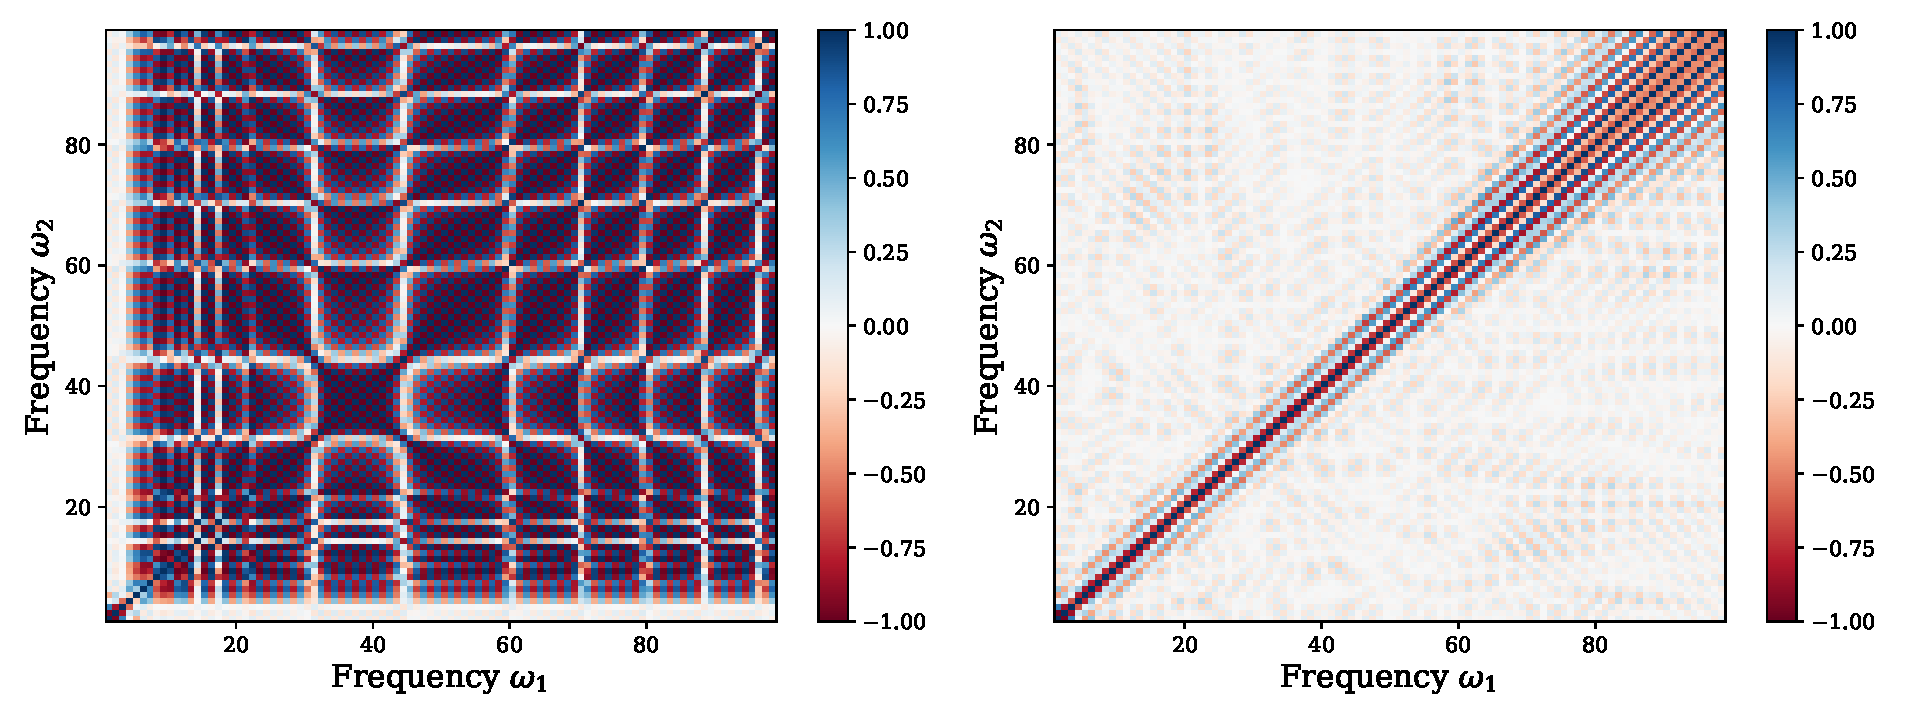
\includegraphics[width=\textwidth]{sinlog_equil_template_correlations_compare_decomp.pdf}
	\caption{Correlations between $f_\text{NL}$ constraints for the enveloped resonance shape $S(k_1,k_2,k_3) = S^\text{equil}(k_1,k_2,k_3) \sin(\omega \log(k_1+k_2+k_3))$ with different $\omega$s. Since the given shape behaves badly in the region outside the tetrapyd but within the cubic domain of (\ref{eqn:basis_expansion}), we observe large off-diagonal correlations in the original Legendre basis expansion (Left). Manually setting the shape function to zero at these unphysical configurations therefore dramatically improves numerical performance (Right). }
	\label{fig:sinlog_equil_template_decomp_comparison}
\end{figure}

On the right-hand side is the result for which the shape function values outside the tetrapyd were manually set to zero during the primordial basis expansion. The modified shape function is still continuous within the cubic domain, since the equilateral shape vanishes on boundaries of the tetrapyd despite its divergence outside of it. We see that this simple trick has dramatically improved the basis' ability to expand highly oscillatory bispectrum templates. The cross-correlations between templates remain small up until $\omega\approx75$, quite similar to what we saw for the sine-log templates. We confirm that it is indeed the bad behaviour of the templates outside the tetrapyd domain during the primordial basis expansion that causes the lack of convergence. We plan to explore this topic further in the future.

\newpage
\section*{Summary}

In this chapter, we presented a thorough review of our work on the high-resolution bispectrum estimator \textsc{CMB-BEst}. Starting with the mathematical framework of our pipeline, we showed that our formalism combines the strengths of conventional approaches to bispectrum estimation; we can handle highly oscillatory functions as accurately as the KSW estimator whilst covering a broad range of models like Modal. In order to tackle the computational complexity, we thoroughly optimised the code at both algorithmic and implementation levels. The code was then parallelised for maximal utilisation of high-performance computing clusters.

With the completed code we performed various tests to validate the integrity of \textsc{CMB-BEst}. We showed that the two different choices of basis functions\textemdash monomials and Legendre polynomials\textemdash give consistent constraints for the standard bispectrum shapes. Furthermore, we compared our results to those from the Modal estimator using the Planck 2018 data and found that they agree on a map-by-map basis. Oscillatory shapes such as the feature and resonance templates were also constrained; by analysing the correlation between the templates with different oscillation frequencies, we showed that our basis can handle oscillatory shapes as accurately as the Planck analysis using the Legendre basis of size $p_\text{max}=30$.

Having validated the pipeline, we provided a proof-of-concept example where \textsc{CMB-BEst} is combined with \textsc{Primodal} to constrain inflation models with non-canonical kinetic terms. The combined pipeline is capable of constraining inflation models directly without using approximate templates. We studied the DBI inflation models while varying the speed of sound parameter to obtain the constraint $c_\text{s}^\text{DBI} \ge 0.056$ with 95\% confidence. We are currently preparing to publish the work presented here as \cite{Sohn2021inprep}.





\clearpage{}
\clearpage{}\chapter{Conclusion}

The standard model of cosmology has been remarkably successful; the CMB power spectrum from Planck, for example, shows an exquisite fit to the $\Lambda$CDM model with only six free parameters. Many questions remain unanswered, however, especially regarding early universe physics. The most widely accepted theory for the early universe is inflation, whose prediction of the scale-invariant primordial spectra has been tested to be consistent with the observed data. Inflation also resolves the horizon and flatness problems present in the vanilla Big Bang cosmology. The simplest scenario of the single-field slow-roll inflation with a canonical kinetic term can explain the current observations, but numerous other physically well-motivated scenarios are yet to be ruled out.

The key to distinguishing different models of inflation is primordial non-Gaussianity. Deviations from the most canonical inflation model leave weak non-Gaussian signatures in the primordial perturbations. These imprints are best captured in the bispectrum of the primordial perturbations. Studying the shape and amplitude of the primordial bispectrum, therefore, allows us to constrain various inflation models directly. The CMB is the ideal probe for this job since its anisotropy depends linearly on the initial density perturbations. The CMB bispectrum hence directly relates to the primordial bispectrum and is used to construct the optimal estimator for the primordial non-Gaussianity parameter $f_\text{NL}$. 

The most recent Planck analysis has constrained $f_\text{NL}$ to great precision using the CMB bispectrum estimator. No primordial source of non-Gaussianity has been found, and $f_\text{NL}$s for the standard shapes are currently consistent with $0$. More interesting `hints' of non-Gaussianity have been found in models with oscillations in the bispectrum. Signals of $3$-$4\sigma$ significance have been found in these models, but scanning over a large parameter space meant that these are not yet conclusive detections. A further investigation using independent and more precise measurements would be extremely beneficial.

The next generation of CMB experiments is anticipated to measure the polarisation of the CMB with greatly enhanced sensitivity. Given that the Planck constraints on oscillatory models benefited much more from the inclusion of polarisation data than other shapes, we predict that the constraining power would benefit immensely from the future CMB data. Our work presented in Chapter 4 forecasts that the most sensitive CMB Stage-4 experiment specification is expected to yield a factor of 1.7-2.2 times more stringent constraints compared to Planck.

Despite the bright prospects and growing interest in constraining oscillatory models, a large part of the model and parameter space are currently unconstrained due to numerical and computational difficulties. The CMB bispectrum estimation is a challenging task where the na\"ive computation is practically impossible. There are two main approaches to this: KSW and Modal.

The KSW estimator exploits the inherent separability of the primordial bispectrum template and can accurately constrain even highly oscillatory shapes but is restrictive in the type of bispectrum shapes it can handle. On the other hand, the Modal estimator uses separable mode functions to expand the primordial and late-time bispectra and hence is able to constrain a wide range of non-separable shapes. However, dealing with high-frequency oscillations is challenging for Modal because there are two separate basis sets\textemdash primordial and late-time\textemdash to consider; high-frequency primordial basis functions lose a lot of their features during the projection, making it hard to expand them using the late-time basis functions accurately.

Our novel approach to the CMB bispectrum estimation, \textsc{CMB-BEst}, is designed to combine the strengths of the KSW and Modal estimators, and hence is suitable for constraining general oscillatory models using future CMB data. We use the primordial basis expansion to decompose the given bispectrum shape into separable terms like Modal but then apply a KSW-like method to obtain constraints on each of them. \textsc{CMB-BEst} works for general basis sets and contains the KSW estimator as a sub-case.

The main strength of \textsc{CMB-BEst} lies in its flexibility and accuracy; the code can take general basis functions which get projected using an exact analytic form. This would be especially useful for studying general bispectrum shapes with high-frequency oscillations that are currently unconstrained due to practical difficulties in numerical calculations.

The \textsc{CMB-BEst} pipeline is, however, computationally more costly than both the KSW and Modal ones. We therefore invested a significant amount of time optimising the code at both algorithmic and implementation levels. The code was then parallelised on multiple levels to fully benefit from the modern computing architecture. The total runtime has improved many orders of magnitude throughout this process. The completed code has then thoroughly tested against the Modal pipeline used in the Planck 2018 analysis. We found that the results are consistent with Planck map-by-map using 140 simulated maps, for the standard shapes as well as the feature and resonance templates.

\textsc{CMB-BEst} has been validated and is now in the exploitation phase. Working in collaboration with the authors of \textsc{Primodal}, we developed a fluid pipeline where a given inflationary Lagrangian can be directly constrained without the use of approximate templates. This allows a fast and accurate constraint to the specific model under consideration. As a proof-of-concept example, we presented work on constraining the DBI sound speed in Chapter 5, where we obtained $c_\text{s}^\text{DBI} \ge 0.056$ with 95\% confidence. The combined \textsc{Primodal}+\textsc{CMB-BEst} pipeline can perform similar scans on other theoretical parameters, which we plan to do in the near future.

We further demonstrated that \textsc{CMB-BEst} can indeed handle high-frequency oscillations of the resonance-type bispectra more stably compared to Modal. Its resolving power is limited only by the accuracy in its primordial basis expansion, unlike Modal which also depends on the late-time counterpart. Our next goal is to develop and utilise specialised basis sets tailored to highly oscillatory bispectrum shapes of interest. 

There are currently two main routes for improvement for \textsc{CMB-BEst}. First, the code can be generalised to incorporate the E-mode polarisation data. Implementing this should be straightforward using an orthonormalisation defined in Chapter 4. The additional computational complexity involved in the extra set of spherical harmonic transforms for polarisation is expected to be subdominant and have a small impact overall. Second, we plan on improving the current method used for the decomposition of a given primordial shape function. We will investigate further the effect of the integration domain, as we saw from the example of the DBI resonance models in Chapter 5. We note that this concerns only the last step of the pipeline and the main parts of the bispectrum estimation remain unaffected.

It is truly an exciting time to be researching cosmology. Numerous future experiments will soon provide us with ever more immense and accurate measurements of the observable universe. We believe that the work presented here will add to the community's continued efforts to better understand the universe we live in.
\clearpage{}






\listoffigures

\listoftables

\begin{spacing}{0.9}



\bibliographystyle{JHEP}
\bibliography{References/references} 








\end{spacing}



\begin{appendices} 



\end{appendices}

\printthesisindex 

\end{document}
